\documentclass[12pt]{book}

\usepackage[utf8]{inputenc}
\usepackage[doublespacing]{setspace}

\usepackage{amsmath}
\usepackage{amsfonts}
\usepackage{mathptmx}
\usepackage{mathrsfs}

\usepackage{graphicx}
\usepackage[left = 1in, top = 1in, right = 1in, bottom = 1in]{geometry}
\usepackage{caption}
\usepackage{subcaption}
\usepackage{times}
\usepackage{xcolor}
\usepackage{cite}
\usepackage{wrapfig}
\usepackage[section]{placeins}
\usepackage{breqn}
%\usepackage{endfloat}

\newcommand{\tens}[1]{{\ensuremath{\mathchoice
                     {\mbox{$\displaystyle\mathsf{#1}$}}
                     {\mbox{$\textstyle\mathbf{#1}$}}
                     {\mbox{$\scriptstyle\mathsf{#1}$}}
                     {\mbox{$\scriptscriptstyle\mathsf{#1}$}}}}}

\graphicspath{{figures/}}

\title{PhD dissertation}
\author{Nikhil Karthikeyan}
\date{August 10, 2025}

\begin{document}

\begin{titlepage}
\begin{center}

\vspace*{3cm}

\Large
\textbf{Lattice Boltzmann simulations of magnetically responsive anisotropic particle stabilized emulsions}

% \vspace{0.5cm}

% \large
% Characterizing the effect of magnetic fields  formation kinetics, rheology and particle arrangement of bijels under the infleunce of magnetic fields

\vspace{0.5cm}
\textbf{Nikhil Karthikeyan} \\
\textbf{Schiller Research Group}

\vspace{3cm}

PhD Dissertation \\
Department of Materials Science and Engineering \\
Pierre S. Du Pont Hall, 127 The Green, Newark, DE 19716 \\
University of Delaware

\end{center}
\end{titlepage}

\newpage

% \section*{Abstract}
\section*{Abstract}
\pagenumbering{roman}
Porous materials have found greater importance in applications such as water filtration, catalyst supports, battery 
electrodes and bio engineered materials. To accommodate a greater variety of pore sizes and continuous fabrication 
techniques with minimal waste, bottom up synthesis techniques have been gaining in popularity. 

One such bottom up fabrication technique relies on jamming of particle stabilized emulsions into bicontinuous 
interfacially jammed emulsion gels(bijels). However, casting mixture independent microstructure control has not 
been identified, especially applicable in continuous bijel synthesis strategies such as Solvent Transfer Induced 
Phase separation. Stimuli response has been identified as a technique to enable this. This study focuses on utilizing 
stimuli response of bijels stabilized with ellipsoidal microparticles, and the resulting microstructure and rheological 
implications this induces. 

We first identify that upon application of a field to a bijel stabilized with ellipsoidal particles during synthesis, 
microstructure change is observed, not present when analyzing bijels stabilized with spherical particles. Upon 
application of the field, particles reorient to the direction of the field, dragging the interface along with 
them. This causes the bijel to have axially dependent jamming, causing anisotropic microstructures to form.

We then identify that bijels stabilized with ellipsoidal particles have tunable microstructures after jamming. 
This process is dependent upon the initial particle order present in the bijel, as well as the difference 
between the initial and final particle order. We also show that the structural response observed is state 
dependent, meaning that the time of magnetic field application affects the microstructure change observed.

\newpage

\section*{Acknowledgements}

In the development of this dissertation, I extend my deepest gratitude to Dr Ulf Schiller whose support, motivation and 
opportunities have been indispensible during my PhD. I believe his approach to mentorship, methodical problem solving 
strategies, depth and breadth of knowledge have been invaluable sources of inspiration for this research as well as 
motivating myself to strive towards those ideals. I would also like to thank members of my committee, especially 
Dr Arthi Jayaraman from the University of Delaware and Dr Olga Kuksenok from Clemson University for their mentorship 
and motivation that pushed me to increase my breadth of knowledge and to think outside the box.

Listing everyone I am grateful for who have provided me non-academic support would be too long for this page 
although I shall try to summarize this. I am grateful to my family, with whom I may not be the best at 
discussing my future plans, but they have been an indispensible source of support during my time away from home. 
I am thankful to my lab members especially for adding brief moments of levity during my PhD and giving me the 
opportunity to be a part of their own journey in graduate school. Thank you to everyone who has been with me 
through thick and thin, and to many more celebrations of our achievements. 

\newpage

\tableofcontents
\thispagestyle{empty}

\newpage

\listoffigures

\newpage

\listoftables

\newpage

\pagenumbering{arabic} 
\setcounter{page}{1}

\chapter{Stimuli response and its applications in porous materials}
% \begin{itemize}
%     \item What is a porous material? 
%     \begin{itemize}
%         \item What makes them different to non-porous materials?
%         \item Why do their differences make them industrially relevant?
%         \item What are some synthesis techniques that exist?
%         \item What are weaknesses with those synthesis techniques?
%     \end{itemize}
%     \item What is a particle stabilized emulsion
%     \begin{itemize}
%         \item Why are they interesting for porous material applications?
%         \item What is a bijel?
%         \item How are bijels relevant to porous materials?
%         \item Fabrication techniques that are proposed which allow large scale bijel fabrication
%         \item microstructure control in those applications
%     \end{itemize}
%     \item Purpose of study
%     \begin{itemize}
%         \item Three aims of the study 
%         \item significance of study
%         \item assumptions and limitations of the study
%     \end{itemize}
%     \item Summary of motivation, purpose and research aims
% \end{itemize}

% \textcolor{blue}{
% \begin{itemize}
%   \item Explain what is a porous material and the advantages they have in their applications compared to non-porous materials 
%   \item Detailed description of their applications and why we are interested in stimuli responsive porous materials 
%   \item Overview of porous material synthesis techniques and what are some areas where there is room for improvement (Definition of critical issues)
%   \item Explain what emulsion templating is and the specific advantages it has over other techniques. Recall where it has been used to great effect
%   \item Explain how bijels fit into emulsion templating and how they offer advantages to standard emulsion templates
%   \item Explain how bijels have been manufactured
%   \item Linking stimuli response as a way to add additional functionality to bijels and identifying how to process them more effectively
%   \item Explain why magnetic fields are interesting in this case
%   \item Explain what is a bijel, how they have been synthesized and some hints at past work for controlling their microstructure (literature review)
%   \item Explain how bijels and stimuli response can address the shortcomings addressed in the previous section (Research objectives)
% \end{itemize}
% }

\section{Introduction}
\label{section:introduction}

Porous materials are defined as materials that contain pores or voids within their structure where no material is present. 
Homogeneous materials in contrast have a uniform structure with no pores. These pores vary in shape and distribution, with materials 
being categorized by pore size per IUPAC as $(L)$ as microporous $(L < 2nm)$, mesoporous $(2nm < L < 50nm)$ and macroporous materials 
$(50nm < L)$. \cite{sing_reporting_1985} The presence of these pores increases the surface area to volume 
ratio of porous materials compared to their homogeneous counterparts. A common experimental technique used to estimate the surface area 
of a porous material derived from Brunauer-Emmett-Teller(BET) theory shows that porous materials can have surface areas more than a 
hundred times larger than homogenous materials, dependent upon the pore size and pore size distribution. \cite{shimizu_surface_2022}

In addition to the pore size and its distribution within the material, the arrangement of pores within the material contribute to the 
performance of the synthesized material, commonly measured using the tortuosity. Tortuosity here is defined as the path length between 
two points divided by the euclidean length between those points. A tortuosity larger than one implies that the path length is longer 
than the euclidean length, and vice versa if the tortuosity if less than one. Highlighting the confluence of these factors are the 
large variety of tailored microstructures for various applications. Each of the specified pore length scales have their unique uses, 
such as microporous materials being used as zeolites and photonic bandgap materials while macroporous materials facilitate greater 
transport properties, suitable in applications such as battery electrodes and drug delivery systems. \cite{chen_tortuosity_2020, 
ebner_tortuosity_2014} This increased surface area to volume ratio enhances the properties of the base material in applications such 
as catalysis, battery electrodes and drug delivery systems among many more making them valuable microstructures. 
\cite{cha_bicontinuous_2019, samdani_bicontinuous_2017, thorson_bijel-templated_2019, zhao_highly_2014}

\begin{figure}
    \centering
    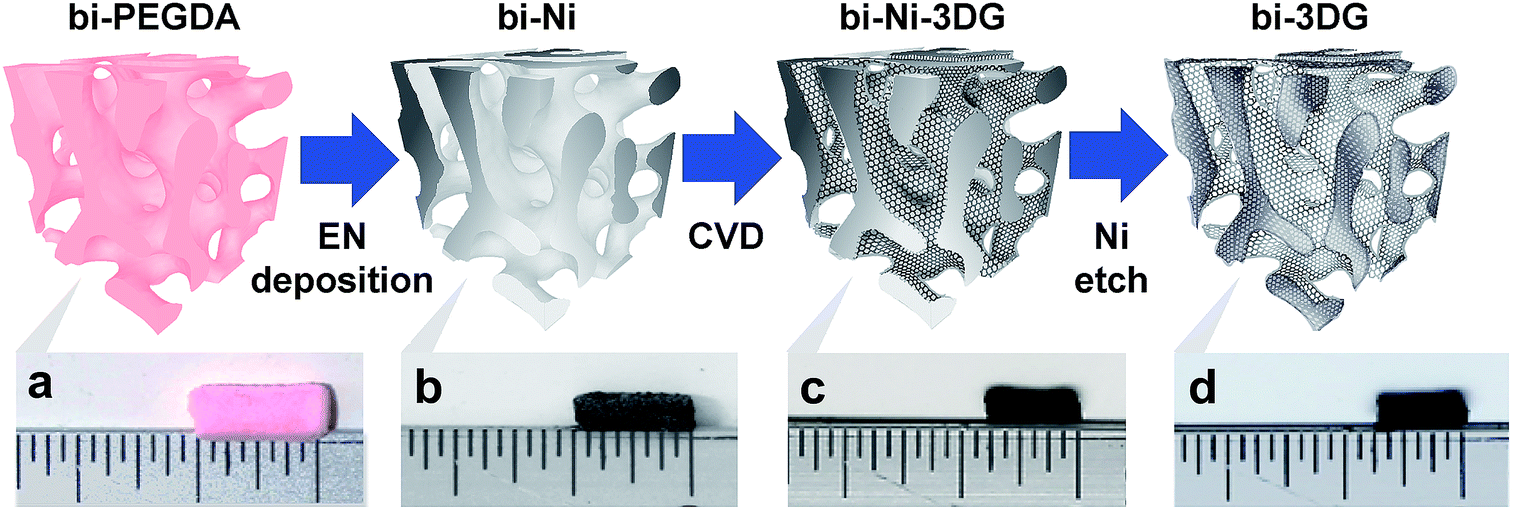
\includegraphics[scale = 0.5]{figures/introduction/bijel_templating.png}
    \caption{Fabrication of a graphite oxide battery electrode using bijel template. Reproduced from Garcie et al. under license number 1548092-1. \cite{garcia_scalable_2019}}
    \label{fig:bijel_template}
\end{figure}

Conventionally, porous materials have been synthesized through solvothermal synthesis or pyrolysis used in the synthesis of zeolites and 
activated carbon respectively. With more targeted applications of porous materials, synthesis techniques such as sol-gel synthesis, 
freeze drying and various forms of templating have been utilized to synthesize porous materials from length scales of $10^{-9}m$ to 
$10^{-3}m$. \cite{stein_morphological_2008, ray_comprehensive_2016, cervellere_mesoscopic_2019, garcia-bennett_unique_2020, zhang_emulsion_2019, 
alves-rosa_design_2013} Industry has also taken up techniques such as electrospinning to generate non woven fibers, used in membrane synthesis. 
Templating techniques in particular offer access to various pore length scales, bottom up synthesis and functionality through leveraging various 
physical phenomena. Colloidal templating works through the close packing of particles. Surfactant and polymer templating work through the 
assembly of macromolecules into their equilibrium configurations. Emulsion templating utilizes the phase separation of partially miscible 
liquids to form the pore structure of a porous material. 

Emulsion templating offers access to a large length scale of tunable pore sizes, continuous production through microfluidic junctions or 
other flow media, functionalization through the addition of additives or stabilizers, scope of accessible microstructures and mild synthesis 
conditions. It can further be extended to include heirarchical porosity, further enhancing its utility and fabricated material properties. 
\cite{yang_hierarchically_2017, thompson_hierarchically_2019, wang_morphology_2023} Figure \ref{fig:bijel_template} demonstrates how emulsion 
templating allows bottom up synthesis of hierarchically porous materials, although other examples do exist. 
\cite{garcia_scalable_2019, santiago_cordoba_aerobijels_2020, thorson_bijel-templated_2019, lu_controllable_2020, wang_morphology_2023}

\begin{figure}
    \centering
    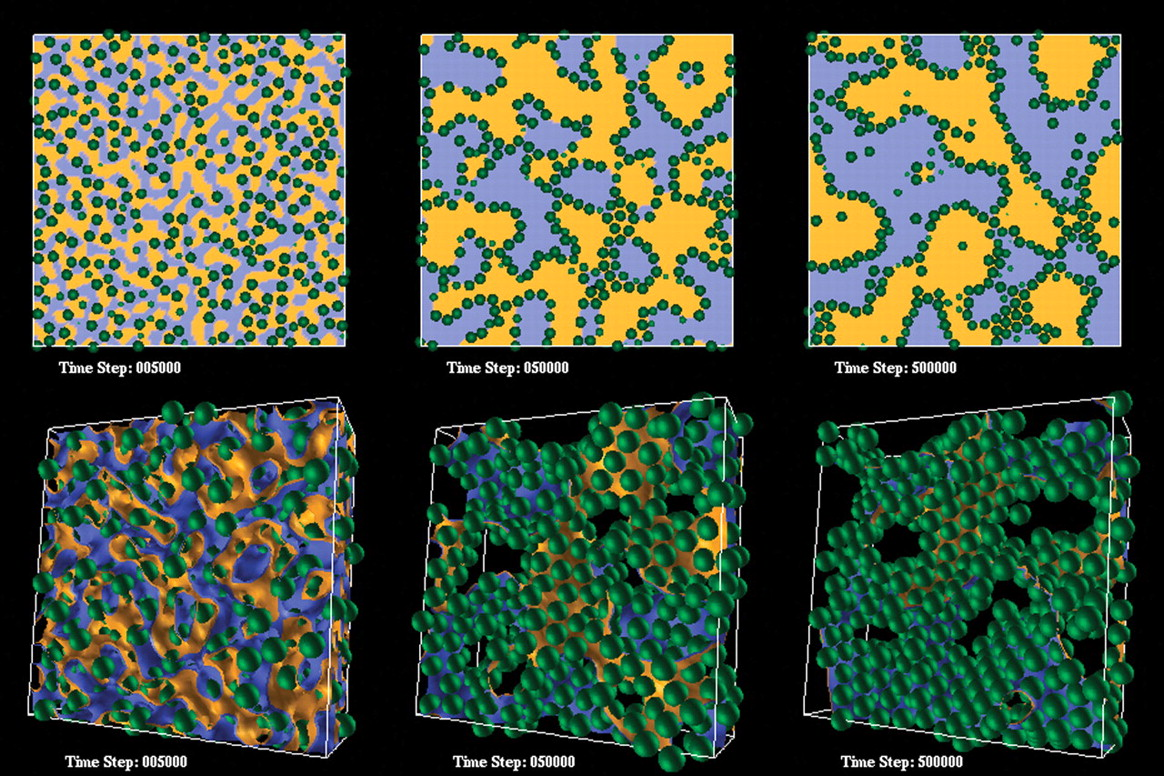
\includegraphics[scale = 0.3]{figures/introduction/bijel_coarsening.jpg}
    \caption{Initiation and arrest of spinodal decomposition as particles adsorb onto the interface, followed by jamming once the 
    interfacial area matches the cross sectional area of the adsorbed particles\cite{stratford_colloidal_2005}. Reproduced from Adhikari et al. 
    under license number 5966820525314.}
    \label{fig:bijel_coarsen}
\end{figure}

One such emulsion microstructure of interest is the bicontinuous interfacially jammed emulsion gel(bijel). 
\cite{stratford_colloidal_2005, herzig_bicontinuous_2007, lee_bicontinuous_2010} Bijels are made by arresting the spinodal decomposition of 
partially miscible liquids, caused by particles adsorbing on the interface and jamming as the cross sectional area of the particles match that 
of the interface, summarized in Figure \ref{fig:bijel_coarsen}. Bijels are of interest due to their co-continuous, tortuous microstructure which 
represent excellent fits for several porous material applications.

Bijels were discovered in simulations in 2005 and experimentally realized in 2007 when a mixture of water and 2-6-lutidine mixed with 
surface modified silica nanoparticles underwent thermally induced spinodal decomposition. \cite{stratford_colloidal_2005, herzig_bicontinuous_2007}
Since then, multiple other casting mixtures and particle chemistry's have been used to fabricate bijels using Thermally Induced Spinodal 
Decomposition (TIPS). \cite{lee_bicontinuous_2010, bai_dynamics_2015} More recently, techniques such as Solvent Transfer Induced Phase 
Separation (STrIPS), Vapor Induced Phase Separation (VIPS), Non-solvent Induced Phase Separation (NIPS), homogenization and liquid in 
liquid printing have been utilized to fabricate bijels, demonstrating the ability for bijels to be synthesized in a continuous process, 
suitable for scale up. \cite{haase_continuous_2015, wang_scalable_2020, cai_bijels_2017, yabuno_preparation_2020, wang_bicontinuous_2023, 
amirfattahi_fabrication_2024} These techniques also offer preparation of bijels in various different shapes and form-factors for various 
uses such as fibers, coatings and capsules, seen in Figure \ref{fig:strips}. \cite{haase_continuous_2015, boakye-ansah_controlling_2020, 
kharal_hightensile_2020, wang_bicontinuous_2023}
\begin{figure}[h]
    \centering
    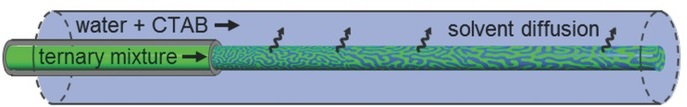
\includegraphics[scale = 2]{figures/literature_review/STRIPPS.jpg}
    \caption{STrIPS in action. Extrusion of the bijel casting mixture into a non-solvent bath, followed by removal of solvent from 
    the casting mixture through diffusion. Reproduced from Haase et al. 2015 under license number 5913140219015. \cite{haase_continuous_2015}}
    \label{fig:strips}
\end{figure}

However, these techniques all depend upon controlling the rate of phase separation, which involve changing the casting mixture composition to 
modify the obtained microstructure. In STrIPS, the obtained bijel microstructure is a function of the flow rate and selected co-solvent, 
selected to change the rate of phase separation. \cite{haase_continuous_2015} This affects material properties such as the mechanical 
performance of the bijel, important in fields such as catalysis where rigidity of the particle monolayer is crucial in ensuring consistent 
performance. \cite{reeves_particle-size_2015, haase_situ_2016, boakye-ansah_controlling_2020} Identification of other techniques that can 
be utilized to modify the microstructure of a bijel would enable bijels to continue using the desired composition of constituents, while 
also adding other unique properties. Stimuli response offers one such road to microstructure modification.

\textcolor{blue}{ADD IN PICTURE FROM THAM 2021 AND CUI 2013 ON EXAMPLES OF STIMULI RESPONSE IN EMULSIONS}

Stimuli response based on pH, external fields and temperature have been used in past works when looking at modifying the microstructure of 
emulsion droplets for enhanced oil recovery, pharmaceutical and cell adhesion. \cite{haase_nanoparticle_2011, tham_magnetophoresis_2021, 
cui_stabilizing_2013, manfredini_limonene--water_2021}  It was shown that external fields can be used to move, control emulsion stability 
and elongate emulsion droplets. \cite{tham_magnetophoresis_2021, cui_stabilizing_2013, melle_pickering_2005} Bijels stabilized spherical 
particles under a magnetic field showed no meaningful microstructure changes. \cite{kim_bijels_2010} Bijels stabilized with spherical 
particles under an electric field showed more promise. \cite{carmack_tuning_2018} However, magnetic fields offer targeted stimuli 
response, allowing even weak fields to incite a response. Magnetic fields non-interaction in many situations offer advantages to many of 
the desired uses of bijels within pharmaceutical or bioengineering applications. \cite{vanoli_bijels_2022, thorson_bijel-templated_2019, thorson_composite_2018} 
These applications can also take advantage of in-situ microstructure modification that would enable tunable drug delivery rates, separations or
catalyst efficiency and permeability improvements in the system. Therefore, identifying schemes that allow modification of the pore size 
and tortuosity without synthesis of a new material would enhance the use case of bijels. 

Anisotropic particles at interfaces have shown self assembly due to the presence of multi-polar pressure fields caused by interface deformation. 
Self assembly has also been shown for ellipsoidal particles at interfaces under magnetic fields. Ellipsoidal particles have also been shown to 
exhibit magnetic field controlled orientations at interfaces, as Bresme and Faraudo showed. \cite{bresme_orientational_2007, davies_interface_2014}
Under magnetic fields, assemblies of multiple ellipsoidal particles have been shown to have energy minima at orientations different from isolated particles,
meaning that the interface coverage of interfaces decorated with ellipsoidal particles can be varied using stimuli response. 
\cite{newton_influence_2014, newton_capillary_2018} Thus ellipsoidal particles at interfaces, whose orientations and packing can be 
controlled through external fields, offer a potential means to control the microstructure of bijels.

Bijels present a bottom up synthesis strategy for porous material templates for hard and soft material applications in a scalable and 
continuous method using STrIPS and other techniques. However, the microstructure control these techniques offer are intrinsically linked 
to the casting mixture composition. Stimuli response offers a way to modify the microstructure of bijels while still maintaining the 
various form factors these continuous synthesis techniques can output. Magnetic stimuli response has been explored in the past using bijels 
stabilized with spherical particles with little success. \cite{kim_bijels_2010} 

With this background, we propose anisotropic particles as a technique to enable microstructure modification of bijels 
upon application of an external field during and after fabrication. This work seeks to identify means to control the bijel microstructure independent 
of the casting mixture composition by utilizing magnetic stimuli on bijels stabilized with magnetically responsive ellipsoidal particles. 
The proposed mechanism of microstructure modification is driven through reorientation of the particles to the applied magnetic field altering 
how the particles pack on the interface. By changing the interfacial packing of the particles, we change when the particles jam, which in turn changes 
the jamming point of the bijel. This mechanism is predicted to be effective during and after synthesis. The processability of bijels fabricated using 
this technique will also be investigated to ascertain how changes in particle packing affect the rheology of the material. An overview of three major 
research aims will be presented below.

\section{Research objective}

% this work seeks to identify means to control the bijel microstructure independent of the casting mixture composition utilizing magnetic stimuli response of anisotropic particles. The proposed mechanism of microstructure modification is driven through reorientation of the particles to the applied magnetic field altering how the particles pack on the interface.

\subsection{Aim 1: Determination of the degree of microstructure changes expected when applying a constant field during bijel formation}
\label{section:aim1_desc}

The jamming point of a bijel controls the obtained microstructure, as shown by previous work comparing the length scale of bijels synthesized 
with different particle volume fractions and particle sizes. \cite{jansen_bijels_2011, reeves_particle-size_2015} It has also been shown how magnetic fields 
can be used to enable self assembly of ansisotropic particles at interfaces and control the interfacial angle between the particle axis of symmetry and the interface. 
\cite{davies_interface_2014, davies_assembling_2014}
On a curved interface with many other particles, it is unknown how multiple particles orienting to a field and having regular structure will affect when and how the bijel 
will jam. \cite{bresme_orientational_2007, davies_interface_2014}

To assess the obtained microstructure upon application of a field during formation of the bijel, homogenous mixtures containing spherical and 
ellipsoidal particles will be subjected to field strengths above and below the critical field strength when particle orientations to the 
interface are controlled by the applied field strength, as calculated by Bresme and Faraudo for the particle aspect ratio. \cite{bresme_orientational_2007, davies_interface_201} This selection of fields 
will allow insight into the controlling mechanisms behind microstructural changes observed, allowing verification of the hypothesis and 
ascertainment where the most control over the microstructure can be exercised.

The average and directional domain sizes in addition to their relation with tortuosity will allow characterization of the microstructural properties 
of the resulting bijel. The nematic order parameter and average interfacial angle will be used to investigate how the application of the 
field affects the particle ordering to each other, and to the interface. Finally, the radial distribution function will be used to assess 
if the orientational changes expected upon field application, affects the packing of the particles on the interface.

\subsection{Aim 2: Microstructure changes and timescales upon application of a magnetic field after formation}
\label{section:aim2_desc}

Particles on the surface of emulsion droplets have been shown to unjam and rejam into new, stable microstructures upon application of 
stimuli. \cite{cui_stabilizing_2013} Magnetic fields applied to bijels stabilized with ellipsoidal particles will facilitate unjamming and rejamming of
the particle monolayer, resulting in microstructure modification of the bijel. Due to local changes in the state of the particles, specifically the 
interfacial ordering in a specific direction and arrangement of particles, we expect that there will be microstructure modification even when the 
magnetic field is switched off. Two techniques of microstructure change are proposed. The first technique is that the adsorption 
energy is so strong that the interface is dragged along with the particles until they rejam in their new location and orientation to the 
field. The second technique is that the particles tilt in place out of the interface, causing domain coarsening before the particles jam 
in their new positions and orientations. The mechanism, derived microstructure change and timescales will be assessed in this aim.

The response of bijels to magnetic fields will be assessed through analyzing how model bijels made with no fields respond to field strengths 
above and below the critical field strength as calculated from Bresme Faraudo theory. The microstructure properties such as the average domain 
size, particle orientation to the field and interface and the Steinhardt 6 fold bond order parameter to examine the spatial relationship of 
the particles to their neighbors. These techniques will allow elucidation of which mechanism is present at which magnetic field strength. 
Additionally, the microstructure changes observed will be characterized and compared to one another to assess how the applied magnetic field 
changes the final microstructure obtained. 

Next, the importance of the initial order of the particle monolayer will also be assessed through increasing the applied field to equal to the 
surface tension forces on bijel templates simulated under various field strengths. The applied field will also be switched off on bijel templates 
simulated under the same field strengths. The same analysis metrics mentioned earlier will be used. Additionally, the microstructures with the 
same difference in applied field,  will be assessed to investigate the reversibility of bijel microstructures. 

\subsection{Aim 3: Rheological characterization of bijels formed under and subjected to a magnetic field}
\label{section:aim3_desc}

In many of the fabrication processes described above, the rheology of the bijel casting mixture is essential. 
\cite{haase_continuous_2015, cai_bijels_2017, amirfattahi_fabrication_2024} Ching showed that rheologically, bijels are 
colloidal glasses percolating in 3D space. \cite{ching_bijel_2022} A shear capillary number, $Ca_s$, is defined that correlates the 
applied strain rate to the capillary forces derived from surface tension. \cite{frijters_effects_2012, yang_capillary_2022} We are interested 
in identifying the effect of the initial microstructure and an applied field on the rheological properties of the bijel.

% $Ca_s = \frac{\eta_{f} \dot{\gamma} L_{1}}{\sigma}$ where $\dot{\gamma} = \frac{u_{LE}}{L_x}$ is the strain rate and 
% $L_1$ is the average domain size. \cite{frijters_effects_2012, yang_capillary_2022} Lower capillary numbers in the range of
%  $ 10^{-7} \geq Ca_s \leq 10^{-5}$ will be utilized. 
% which corresponds to a $Ma << 0.01$ to accommodate the hydrodynamic model utilized.

For this study, the yield stress and viscosity of the bijels will be explored as a function of the initial microstructure under 
various $Ca_s$. The initial microstructure will be derived from bijels stabilized with ellipsoidal particles made with no magnetic field 
and with a field strength equal to the surface tension energy. We then apply constant shear defined with $Ca_s$ to determine the yield stress and non-newtonian
characteristics of the bijel. Previous investigations have revealed that the ordering of particles in the direction of shear change
the rheological behavior significantly compared to unordered systems. Additionally, the domains of the bijel may create additional mechanisms for 
rheological behavior modification which have not been probed in detail yet. 

We will then identify the complex rheology of the bijels, calculating the loss and storage modulus of the bijel microstructures detailed earlier
as a function of the oscillation of shear. The loss and storage modulus detail the viscous and elastic behavior of the bijel respectively, meaning 
that the gel point of the bijel can be established as the point when the storage modulus exceeds the loss modulus. We will pay special attention to the 
state of the particles in all simulations, correlating changes in the properties of the particle to observed rheological events. We will also identify if shear banding
is observed. 

\chapter{Literature Review}
\section{Emulsion stability and microstructures}

When two partially miscible fluids are mixed, they tend to separate into distinct phases to minimize the thermodynamic penalty associated with interfacial formation. 
To inhibit this phase separation, small-molecule surfactants are conventionally employed. A well-known example of such a material is soap, which facilitates the 
emulsification of dirt into droplets suspended in water through mechanical agitation. Surfactants function by reducing the surface tension between the dispersed 
phase (droplets) and the continuous phase (bulk fluid), thereby lowering the interfacial energy penalty associated with phase formation.

The existence of particle-stabilized emulsions has been recognized for over a century, following the independent discoveries by Pickering and Ramsden, who observed dispersed 
oil droplets within a water matrix after vigorous stirring of an oil-water-particle mixture \cite{ramsden_separation_1904, pickering_cxcvi.emulsions_1907}. Unlike surfactants, 
which stabilize emulsions by reducing interfacial tension, particles act as stabilizers by adsorbing at the interface between the dispersed and continuous phases, thereby 
preventing direct contact between them. The Pieranski model, derived from \textcolor{blue}{insert derivation of Pieranski model}, is commonly used to determine the adsorption 
energy of a particle at an interface. It is expressed as $ G_{ads} = \sigma A_{rm} (1 - \cos{\theta_c})^2 $ where $G_{ads}$ represents the free energy reduction upon particle 
adsorption, $\sigma$ is the surface tension between the partially miscible fluids, and $ \theta_c $ is the contact angle of the particle. Particles at the interface are 
generally considered irreversibly adsorbed, even at the nanoscale. For particles larger than 100 nm, the adsorption energy is sufficiently high that thermal fluctuations at 
the interface can be considered negligible \cite{cheung_molecular_2011}.

Following their initial discovery, interest in particle-stabilized emulsions waned for several decades. However, since the 1980s, renewed attention has emerged due to 
their applications in food science. A notable example is the stabilization of water droplets in oil by fat crystals, a process used in margarine production. Particle 
stabilization has also gained interest due to its lower toxicity and the potential for sustainable sourcing, particularly through the use of cellulose or chitin 
particles \cite{fujisawa_nanocellulose-stabilized_2017, tang_stimuli-responsive_2016, kalliola_carboxymethyl_2018}. Moreover, conventional chemical surfactants pose 
environmental concerns, as they can be toxic to aquatic life, acting as xeno-hormones and disrupting reproductive processes 
\cite{kaczerewska_environmental_2020, lechuga_acute_2016}.

Compared to surfactant-stabilized emulsions, particle-stabilized emulsions exhibit greater resistance to coarsening, leading to renewed interest in their applications. 
The microstructural properties of these emulsions were extensively studied in the early 2000s by Lumsdon, Binks, and others. Their findings indicated that the emulsion 
droplet radius follows the relationship $R_e \propto \frac{\phi_w}{\phi_p}$, where $\phi_w$ and $\phi_p$ represent the volume fractions of water and particles, 
respectively \cite{binks_pickering_2001}. Additionally, they identified several factors influencing the microstructure of Pickering emulsions, including fluid concentration 
and particle wettability. Neutrally wetting particles do not impose a preferential curvature on the interface, whereas non-neutrally wetting particles can lead to the 
formation of bridged droplets, capillary aggregates, and other non-spherical microstructures. A notable example is bijels, which are synthesized in systems containing equal 
volume fractions of immiscible fluids and neutrally wetting particles, leading to the formation of tortuous, co-continuous domains.

Bijels are synthesized in systems containing approximately equal fluid volume fractions and neutrally wetting particles to prevent the imposition of preferential 
curvature at the interface \cite{stratford_colloidal_2005, herzig_bicontinuous_2007, lee_bicontinuous_2010, jansen_bijels_2011, velankar_non-equilibrium_2015}. 
Reeves et al. demonstrated that bijels stabilized with nanoparticles exhibit greater stability than those stabilized with microparticles due to enhanced mechanical 
properties and improved interfacial coverage \cite{reeves_particle-size_2015}. 
Furthermore, research by Jansen, Harting, and Hijnen et al. established that the bijel domain size follows the relationship $ L \propto \frac{1}{\phi_p} $ for both 
rod-like and spherical particles. While the proportionality constant depends on particle geometry, this trend has been observed across various particle shapes 
\cite{hijnen_bijels_2015, madivala_exploiting_2009, gunther_timescales_2014, daware_emulsions_2015, loudet_capillary_2005, cheng_shape-anisotropic_2013}.

% While bijels are a relatively new material class, much work has been conducted to elucidate the underlying mechanisms controlling their stability, microstructure and rheology. Many studies focus on how the particle properties play important roles in tuning the properties of bijels. This section will cover a brief overview and summary of literature on the working principle behind particle surfactants, the effect of size and concentration of particles, anisotropic particles in particle stabilized emulsions, microstructure control in various bijel synthesis techniques, stimuli response in bijels and bijel rheology. 

\begin{figure}
    \centering
    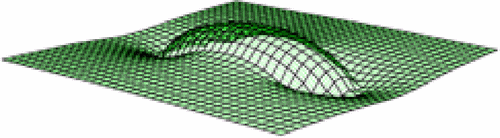
\includegraphics[scale = 0.5]{figures/literature_review/interfacial_curvature.png}
    \caption{Quadropolar capillary interactions around prolate ellipsoidal particles caused by interfacial deformations around the particle. 
    \cite{loudet_capillary_2005} Reproduced from Loudet et al. with license number RNP/25/FEB/088185}
    \label{fig:anisotropic_particle_interface}
\end{figure}

\section{Particle shape anisotropy and synthesis techniques}

Over the past decade, advancements in synthesis techniques have significantly expanded the ability to fabricate particles with anisotropic geometry and surface chemistry. 
The choice of synthesis method depends on the desired particle shape. For example, ellipsoidal particles can be readily produced through the mechanical deformation of 
polymer spheres, while dumbbell-shaped particles can be synthesized using microfluidic devices or emulsion templating. Square-shaped particles, on the other hand, can be 
generated through controlled crystallization \cite{morgan_understanding_2013}. The increasing variety of synthesis methods has reduced geometric constraints when exploring 
potential particle stabilizers for bijels \cite{wu_recent_2016}.

Anisotropic particles exhibit shape-dependent properties due to their ability to induce multipolar interactions by deforming the interface to maintain a mean curvature of 
zero, thereby satisfying the Young-Laplace equation, as illustrated in Figure \ref{fig:anisotropic_particle_interface} \cite{loudet_capillary_2005, cheng_shape-anisotropic_2013}.
This property has been leveraged to facilitate directed assembly and migration through modified capillary forces 
\cite{cavallaro_curvature-driven_2011, read_dimerization_2020, sharifi-mood_curvature_2015}.  

Anisotropic particles have also been shown to exhibit natural liquid crystal like behaviour as shown using Onsager theory. 

When stabilizing bijels, ellipsoidal particles provide greater stability than spherical ones due to their higher cross-sectional area-to-volume ratio, as demonstrated by 
Günther et al. and Hijnen et al. \cite{gunther_timescales_2014, hijnen_bijels_2015}. This enhanced stability arises from additional domain coarsening timescales associated 
with particle reorientation and increased mechanical rigidity, as confirmed by rheological studies \cite{gunther_timescales_2014, daware_emulsions_2015, witt_bijel_2013}. 
Furthermore, particle shape influences both the onset and dynamics of jamming. Studies using graphene plate-like particles have shown that these particles exhibit intrinsic 
elasticity, which affects the conditions under which jamming occurs \cite{imperiali_simple_2014, sun_assembly_2013}.

The orientation of ellipsoidal particles at interfaces is governed by a balance between interfacial capillary forces and external magnetic fields 
\cite{bresme_orientational_2007, davies_assembling_2014}. Theoretical studies and simulations suggest the existence of a critical field strength beyond which particle 
orientation is predominantly dictated by the applied field \cite{bresme_orientational_2007, davies_assembling_2014}. Additionally, both experimental and computational 
studies have shown that steric interactions—modulated by particle orientation and interfacial arrangements—play a significant role in determining the free energy of particle 
assemblies, underscoring the intricate interplay between these forces \cite{morgan_understanding_2013, newton_influence_2014, newton_capillary_2018}.

% The adsorption process is affected by the shape of particles used as they pack differently onto the interface \cite{hijnen_bijels_2015, daware_emulsions_2015,carmack_diverse_2017}. It has also been suggested that adsorption dynamics of ellipsoidal particles at liquid interfaces are driven completely by viscous forces even if the timescales of adsorption are driven by particle properties \cite{Coertjens2017}. Some guiding equations to calculate the interfacial area of an ellipsoidal particle are provided \cite{gunther_timescales_2014, Davies2014}.

\section{Bijel synthesis techniques}

Bijels were first synthesized using Thermally Induced Phase Separation (TIPS) \cite{herzig_bicontinuous_2007, lee_bicontinuous_2010, bai_dynamics_2015}. 
The process begins by identifying a small-molecule or polymer blend with a critical point, referred to as the casting mixture, and preparing it at a composition 
corresponding to this critical point. The casting mixture is then combined with particle surfactants while remaining in a single-phase state. Once the particles 
are homogeneously distributed, phase separation is induced by adjusting the temperature to bring the system into the two-phase region. By ensuring that the 
composition aligns with the critical point, the casting mixture undergoes spinodal decomposition, preventing nucleation and growth.  

TIPS enables batch synthesis of bijels in research laboratories. However, for bijels to become industrially viable, a continuous fabrication process is required—one 
that also allows for the production of various bijel form factors suited to different applications. Solvent Transfer Induced Phase Separation (STrIPS) has been proposed 
as a method to achieve this. In STrIPS, a casting mixture is prepared, consisting of two fluids that form the bijel, a co-solvent, particles, and a surfactant. Phase 
separation is initiated as the co-solvent diffuses out of the bijel. The surfactant is included to maintain bijel stability against Marangoni forces. The casting mixture 
is then extruded into a bath of a non-solvent, which is immiscible with the bijel-forming fluids but miscible with the co-solvent. The diffusion of the co-solvent triggers 
phase separation, leading to bijel formation. The resulting microstructure is influenced by both the surfactant concentration and the flow rate of the casting mixture.

\textcolor{blue}{Description of VIPS}

Vapor Induced Phase Separation(VIPS) has also been identified as a technique for continuous fabrication of bijels. \cite{wang_scalable_2020} A quarternary casting mixture
containing particles, solvent and two partially miscible liquids is prepared. The solvent and liquid species are carefully selected to ensure that removal of the
solvent will cause phase separation of the two partially miscible liquids. One system that has been used is the water/hexanediol-diacrylate solvated by ethanol.
Selection of the composition of the system facilitates crossing of the binodal through the critical point, causing phase separation through spinodal decomposition.
This technique has been used to fabricate thin films of bijels blade and spray coated onto substrates.

\textcolor{blue}{Description of homogenization}

Instead of relying upon spinodal decomposition to generate the bijel morphology, homogenization uses shear to join phase separating domains, resulting in a 
structure that has the properties of a bijel even if not fabricated from fluids undergoing spinodal decomposition. \cite{huang_bicontinuous_2017, cai_bijels_2017} 
This method is primarily used for nanoparticles under $50$ nm and it has been shown to work for multiple particle geometries. This method relies upon
shear to cause limited coalescence of droplets. As coarsening occurs, particles adsorb on the interface and when the interfacial area matches the area of the
adsorbed particles, the microstructure jams. Tuning of the method can be done through modifying the contact angle of the particles at the interface as well as
the viscosity of the fluids. 

\textcolor{blue}{Description of liquid in liquid printing}

Enter something about this method. \cite{amirfattahi_fabrication_2024}

\section{Rheological models and shear response of bijels}

Bijels undergoing constant shear demonstrate shear thinning behavior which at moderate shear rates can be described reasonably well using the Herschel-Buckley
model. \cite{macmillan_rheological_2019, wang_morphology_2023} At higher shear rates, the bijel microstructure is destroyed and the viscosity becomes newtonian. 
\cite{cai_bijels_2017,bonaccorso_shear_2020}. Figure \ref{fig:bijel_under_shear} illustrates the findings of Bonnacorso et al., which observed that when a bijel 
stabilized with hard-sphere-like particles is subjected to shear, the particles initially align with the shear direction before detaching from the interface 
\cite{bonaccorso_shear_2020}. Investigating the impact of particle alignment on rheology, prior studies in suspension rheology have shown that colloidal systems 
with hard-sphere interparticle interactions undergoing constant shear exhibit shear banding—where particles order in the shear direction at moderate shear rates—resulting 
in shear thinning \cite{vermant_flow-induced_2005, brader_nonlinear_2010}. 

\begin{figure}
    \centering
    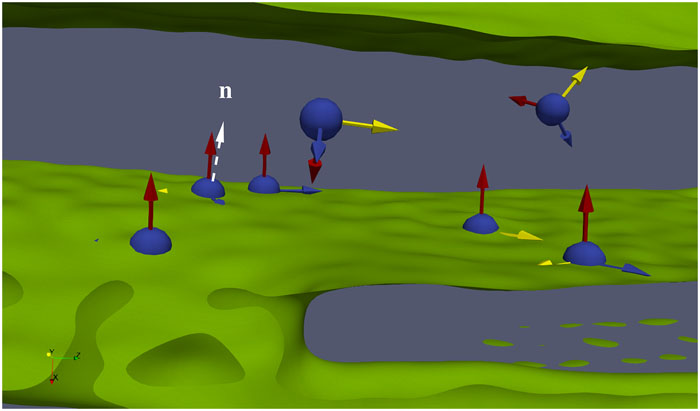
\includegraphics[scale = 2]{figures/literature_review/bijel_under_shear.jpeg}
    \caption{Schematic of a bijel with hard-sphere particles undergoing shear, demonstrating migration and detachment of particles at the interface. 
    \cite{bonaccorso_shear_2020}}
    \label{fig:bijel_under_shear}
\end{figure} 

Studies on complex bijel rheology have demonstrated gel-like characteristics when the storage modulus exceeds the loss modulus \cite{lee_making_2013, bai_dynamics_2015}. 
Ching and Mohraz further showed that the rheological behavior of bijels closely resembles that of a 2D colloidal glass percolating in 3D space, based on comparisons of 
linear viscoelasticity with colloidal gels composed of strongly attractive particles \cite{ching_bijel_2022}. Key characteristics of glasses include the presence of a 
yield stress, viscoelastic behavior, and a glass transition point \cite{pham_yielding_2008, weeks_introduction_2017}. Yield stress corresponds to the applied stress at 
which the particle monolayer undergoes irreversible structural changes \cite{pham_yielding_2008}. Viscoelasticity arises when the monolayer exhibits both solid and 
liquid-like behavior, depending on the timescale of the applied stress \cite{pham_yielding_2008}. The glass transition point is marked by a dramatic slowdown in the 
monolayer's dynamics \cite{weeks_introduction_2017}. 

% \textcolor{blue}{https://www.mdpi.com/2311-5521/5/3/150}

% \section{Colloidal glasses}

% \begin{itemize}
%     \item https://pubs.acs.org/doi/10.1021/acsmacrolett.6b00826
%     \item Add stuff on dynamic heterogeneity
%     \begin{itemize}
%         \item https://pubs.rsc.org/en/content/articlelanding/2012/sm/c2sm25267h
%     \end{itemize}
%     \item Add stuff on particle jamming
%     \begin{itemize}
%         \item https://journals.aps.org/rmp/pdf/10.1103/RevModPhys.82.2633
%     \end{itemize}
%     \item Add stuff on cooperatively rearranging regions
%         \begin{itemize}
%             \item https://doi.org/10.1038/ncomms4829
%             \item https://journals.aps.org/prl/abstract/10.1103/PhysRevLett.110.188301
%             \item https://journals.aps.org/prl/abstract/10.1103/PhysRevLett.107.065702
%         \end{itemize}
%     \item Add stuff on reentrant glass phenomena 
%     \begin{itemize}
%         \item https://doi.org/10.1209/0295-5075/86/58001
%     \end{itemize}
% \end{itemize}

\section{Stimuli response in particle stabilized emulsions}

Kim et al. found that strong magnetic fields do not significantly alter the microstructure of a bijel stabilized with spherical particles, as the particles orient 
to the field without affecting interface ordering. \cite{kim_bijels_2010} In contrast, Carmack and Millet demonstrated that polarizable fluids and particles under 
an electric field show significant microstructural changes, with particles self-assembling into chains and forming cylindrical domains parallel to the applied field, 
thus modifying the microstructure. \cite{carmack_tuning_2018}

\section{Lattice Boltzmann Method}

The Lattice Boltzmann Method (LBM) is an evolution of preceding lattice gas automata techniques, which is a discretization of the Boltzmann equation of motion for 
molecules. This means that unlike traditional CFD techniques such as FDM, VOF or level set methods, LBM is a psuedo-molecule method that tracks the evolution of a 
particle distribution function within grid cells evolved through a discretized Boltzmann equation of motion. Macroscopic variables such as fluid density and 
velocity are recovered from the particle distributions through appropriate moment integration, and the Navier Stokes equation at the incompressible limit can be 
obtained through a Chapman-Enskog expansion of the LBM. The LBM has become an attractive tool for meso-scale CFD simulations due to its ease of algorithm 
implementation, highly parallelizable nature and ease of boundary condition implementation, allowing coupling to other physically relevant systems such as 
particles with varieties of potentials, external fields and deformable bodies.

The particle distribution function described earlier is advected on a pre-constructed lattice stencil, commonly denoted as DnQm where n and m represent the 
number of dimensions and directions in the stencil. Common stencils include the D1Q5, D2Q9 and D3Q19 stencil, all of which recover mass and momentum conservation. 
For energy conservation, a higher order stencil such as D3Q27 is necessary. The D2Q9 and D3Q19 stencils have 8 and 18 populations respectively that include 
connections to nearest and next nearest neighbour points, in addition to a central rest point. 

The LBM is composed of a collision and advection step. In the advection step, the populations at each grid point are propagated to adjacent points in accordance 
with the chosen stencil. During the collision step, the particle population distribution is relaxed towards an equilibrium with a collision operator, at a 
specified relaxation rate. The collision operator can have multiple forms based on how many relaxation rates are used although the most common variant is the 
Single Relaxation Time (SRT) collision operator, more commonly known as the Bhatnagar-Gross-Krook (BGK) collision operator. Owing to its stability in low Mach 
and Reynolds numbers and simplicity of implementation, the BGK operator is often used in common particle laden flow and soft matter scenarios. 
\cite{bhatnagar_model_1954} These limitations are present owing to the implicit link between the fluid properties and the relaxation rate necessitating 
relaxation rates above 0.5, and to ensure fluid incompressibility from an equation that intrinsically simulates a compressible fluid. To get over these 
limitations, Two Relaxation Time (TRT) and Multiple Relaxation Time (MRT) operators also exist, expanding the possible application of the LBM to visco-elastic 
flows and implementation of fluctuating hydrodynamics in the LBM. \cite{liu_simulation_2023, adhikari_fluctuating_2005}

Four primary techniques to model multicomponent or multiphase systems exist in the LBM literature. A quick review of the Shan-Chen or 
interparticle potential model  will be provided here from the perspective of a binary mixture. Additionally, the names and descriptions of 
other techniques will be described as well. The interparticle potential model or Shan-Chen model that adds a non-local density dependent force 
between two species, effectively modelling non-ideal mixing and recovering the Cahn-Hilliard equation. To alleviate the standard Shan-Chen implementations 
weaknesses of not being thermodynamically consistent and reducing the existence of spurious velocities, 

In addition to the Shan-Chen model, the color gradient model, free energy model and interface tracking technique all 
allow for simulations of various types of multiphase and/or multicomponent flows. The color gradient model proposed by Rothman and Keller and 
implemented by Gunstensen et al relies upon modelling two particle distributions. These represent a binary fluid mixture with the collision step 
able to recover the hydrodynamics and non-ideal mixing dynamics. The free energy model utilizes phase field theory and constructs a free energy 
functional to recover interfacial dynamics and effects in a thermodynamically consistent manner. Often, a square gradient free energy is used for 
simplicity and ease of implementation. The mean field theory 

The non-ideal mixing dynamics are recovered during the "recoloring" step, of which the technique proposed by Latva-Kokko and Rothman is more commonly 
used for soft matter flows. \cite{liu_multiphase_2016}

\chapter{The multicomponent Lattice Boltzmann Method}
\label{section:methods}

This work uses a multicomponent Lattice Boltzmann Method (LBM) to simulate the hydrodynamics of two partially miscible, 
incompressible fluids as implemented in LB3D. The LBM solves the continuity and Navier-Stokes equation at low
Mach and Reynolds numbers for the fluid, defined as, 

\begin{equation}
    \begin{split}
    \frac{\partial\rho}{\partial t} + \nabla\cdot\left(\rho\vec{u}\right) &= 0 , \\
    \frac{\partial\vec{u}}{\partial t} + (\vec{u}\cdot\nabla)\vec{u} &= - \frac{1}{\rho} \nabla p + \nu \nabla^2 \vec{u} ,
    \end{split}
\end{equation}

incorporating density $(\rho)$, viscosity $(\eta)$, velocity $(u)$, pressure $(P)$, and 
body force $(F_{body})$. \cite{qian_lattice_1992, chin_lattice_2002, nourgaliev_lattice_2003} The Shan-Chen pseudopotential
model is used to simulate the Cahn-Hilliard equation, defined below

\begin{equation}
    \begin{split}
    \frac{\partial\phi}{\partial t}+\nabla\cdot\left(\phi\vec{u}\right) &= \nabla \cdot \left( \Gamma  \nabla\phi \right)
    \end{split}
\end{equation}

where $c^k$, $M^k$ and $u^k$ is the concentration, mobility and velocity of species $k$ respectively while $\mu$ is the free energy of system. 
\cite{shan_lattice_1993, shan_simulation_1994, he_lattice_1997, he_discrete_1998}

Particle dynamics include Hertzian contact and lubrication forces, tracked with classical Newtonian mechanics, while 
particle-fluid coupling involves momentum exchange to simulate viscous dissipation. Particle-particle magnetic interactions are modeled using dipole 
interactions. \cite{davies_interface_2014, xie_direct_2017, xie_controllable_2021} A more detailed description of the model is 
provided in the following sections

\section{Hydrodynamics} 
\label{section:lbm_hydrodynamics}

The lattice boltzmann method works by evolving a population distribution $f_{i}(\mathbf{x}, t)$ on a cubic lattice with 
timestep $\Delta t$ with lengthscale $\Delta x$. \cite{qian_lattice_1992, succi_lattice_2018, he_theory_1997} The D3Q19 
velocity set is used in this work with the indexes $i$ represent each of the 19 velocities and converves mass and momentum 
conservation to the second order. It can be seen in Figure \ref{fig:d3q19_lattice}. The algorithm is split into the 
collision step where the populations on each lattice grid cell are relaxed towards an equilibrium, followed by the 
advection step where populations in each velocity direction are propagated with velocity $\mathbf{c_i}$. 

The collision step occurs using a single relaxation time Bhatnagar-Gross-Krook (BGK) collision operator at relaxation 
rate $\tau$. \cite{bhatnagar_model_1954, qian_lattice_1992} The combined collision and advection LBM is expressed below 
in equation \ref{eq:LBM_BGK}

\begin{equation}
    f_{i}(\mathbf{x} + \mathbf{c}_{i}\Delta t, t + \Delta t) = f_{i}(\mathbf{x}, t) - \frac{1}{\tau}(f_{i}(\mathbf{x}, t) 
    - f_{i}^{eq}(\mathbf{x}, t))
    \label{eq:LBM_BGK}
\end{equation}

The BGK operator limits simulations to low reynolds number and mach numbers to prevent numerical instabilities. 
\cite{qian_lattice_1992} The kinematic viscosity if using the BGK operator is defined as 
$\nu = c_s^2(\tau - \frac{\Delta t}{2})$. The equilibrium distribution is obtained from a taylor expansion of the 
Maxwell-Boltzmann distribution to the second order. \cite{he_theory_1997, succi_lattice_2018} This is shown in equation 
\ref{eq:LBM_Feq}.

\begin{equation}
    f_{i}^{eq}(\mathbf{x}, t) = w_i\rho(1 + \frac{\mathbf{c_i} \cdot \mathbf{u}}{c_s^2} + \frac{(\mathbf{c_i} \cdot 
    \mathbf{u})^2}{2c_s^4} + \frac{\mathbf{u} \cdot \mathbf{u}}{2c_s^2})
    \label{eq:LBM_Feq}
\end{equation}

\begin{figure}[h]
    \centering
    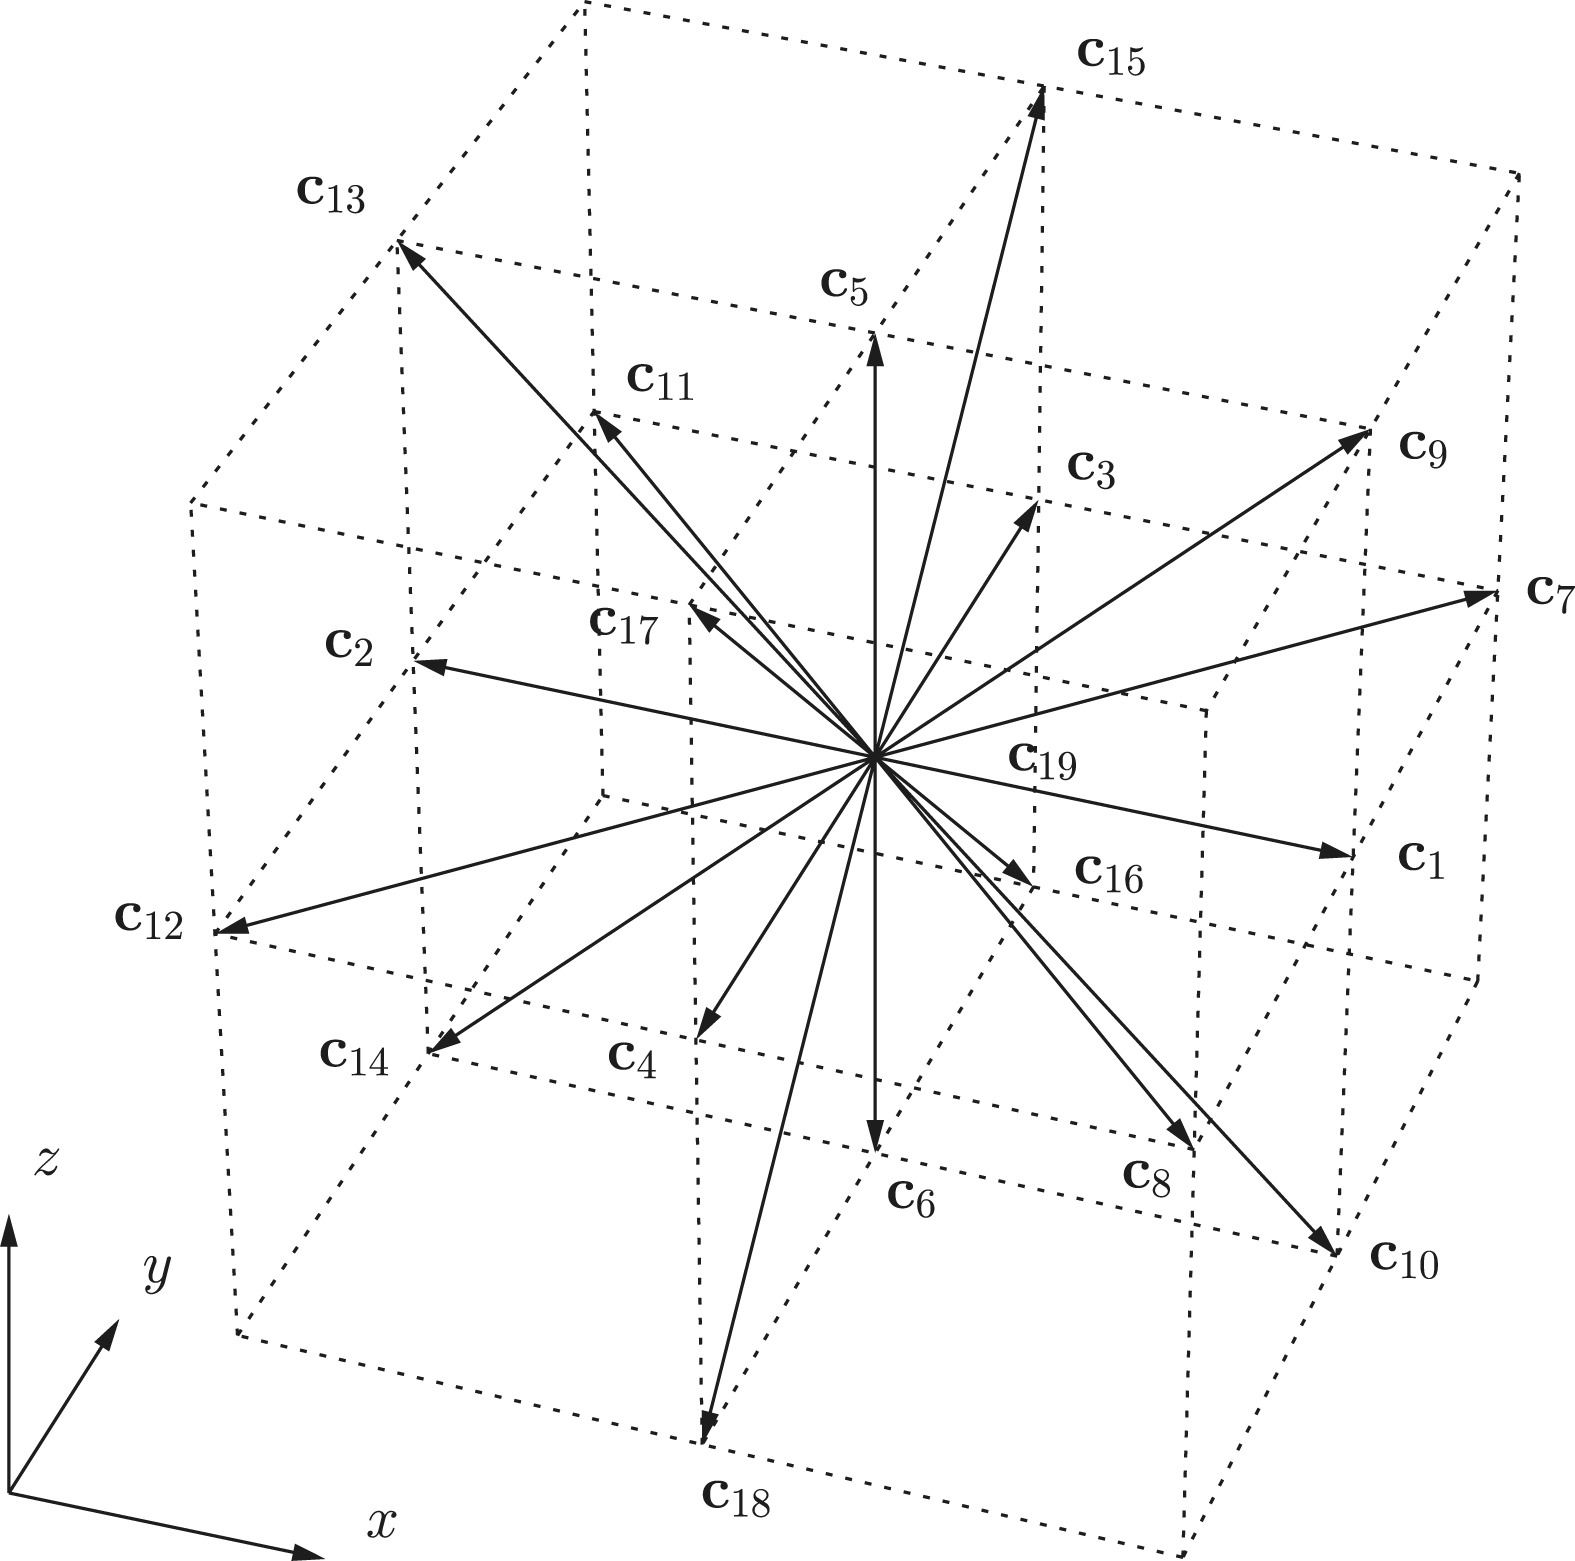
\includegraphics[scale = 0.7]{figures/methods/d3q19_lattice.jpg}
    \caption{D3Q19 lattice demonstrating the rest, nearest and next nearest direction that correspond to the 19 
    directions $(i)$ of the lattice with lattice velocity $c_{i}$. \cite{schmieschek_lb3d_2017} Reproduced from 
    Schmieschek et al. under the Creative Commons license.}
    \label{fig:d3q19_lattice}
\end{figure}

$\rho$ and $\textbf{u}$ in Equation \ref{eq:LBM_Feq} are defined as the macroscopic parameters for density and velocity 
and can be calculated from the mass distribution using $\rho = \sum f_i$ and $\rho \mathbf{u} = \sum f_i \mathbf{c}_i$ 
respectively. Using the Chapman-Enskog expansion, the Navier-Stokes equation at the incompressible limit at low mach
numbers can be recovered. \cite{qian_lattice_1992, he_lattice_1997} The regime accessible through this method is suitable 
for simulations in this work as the $ 1 \leq Re \leq 100 $ and the mach number, $Ma < 0.01$, fulfilling the stability 
criterion and usage requirements for the presented hydrodynamic model.

\section{Non-ideal mixing}
\label{section:lbm_non_ideal_mixing}

The SC model mimics Cahn-Hilliard type behaviour through a force applied from the other fluid species $k'$ in adjacent 
cells $\mathbf{x'}$ on fluid species $k$ at point $\mathbf{x}$. \cite{shan_lattice_1993, shan_simulation_1994, 
shan_multicomponent_1995, he_discrete_1998, jansen_bijels_2011, chin_lattice_2002} Both fluid species are defined
 by their own distribution equation defined in Equation \ref{eq:LBM_BGK} The strength of this force is controlled 
 through an interaction parameter, $g_{kk'}$ with no contribution from self interaction of the fluid as these are 
 set to zero. The SC force can then be written out in Equation \ref{eq:sc_model}.

\begin{equation}
% F_{k}^{SC}(\mathbf{x}, t) = -\Psi^{k}(\mathbf{x}, t)\sum_{k'}g_{cc'}\sum_{\mathbf{x'}}\Psi_{k'}(\mathbf{x'}, t)(\mathbf{x'} 
% - \mathbf{x})
\vec{F}_k(\vec{x}) \Delta t = - \sum_{k'} \sum_i \frac{w_i}{c_s^2} g_{kk'} \psi_k(\vec{x})\psi_{k'}(\vec{x}+\vec{c}_i) \vec{c}_i
\label{eq:sc_model}
\end{equation}

An effective mass of each fluid at node $\mathbf{x}$ is used in place of the actual density to scale it between zero 
and one and is defined as $\psi^{k}(\mathbf{x},t) = \rho_{0}\left[1 - \exp(-\frac{\rho^{k}(\mathbf{x}, t)}{\rho_{0}})\right]$. 
In this model, the SC force is incorporated into the macroscopic velocities that are then used to calculate the equilibrium
distribution $f_{i}^{k, eq}$ for fluid $k$, defined as,

\begin{equation}
\vec{u}_k^{\text{eq}} = \vec{u}' + \frac{\tau_k}{\rho_k} \vec{F}_k
\end{equation}

Where $\vec{u}'$ is defined as the common grid velocity and is calculated from $f_i^k$ below

\begin{equation}
    \sum_k \frac{\rho_k}{\tau_k} \vec{u}' = \sum_k \frac{1}{\tau_k}\sum_i f_i^k\vec{c}_i
\end{equation}

This recasting of the velocity ensures that in the absence of forces, the total momentum of the system is conserved. 

\section{Suspended particle dynamics}
\label{section:lbm_colloids}

Suspended particles will be coupled to the LB fluid based on the work conducted by Ladd. \cite{ladd_numerical_1994, 
aidun_direct_1998, ladd_lattice-boltzmann_2001} The particles follow Newtonian mechanics with the particle force and
rotational inertia defined using differential equations

\begin{equation}
    \begin{split}
    \vec{F_p} = m_p \frac{\vec{u}_p}{dt} , \\
    \vec{D_p} = \mathbf{J}_p \frac{\vec{\omega}_p}{dt} ,
    \label{eq:md}
    \end{split}
\end{equation}

$\mathbf{F_p}$ and $\mathbf{D_p}$ represent the force and torque acting on a particle with mass $m_p$ and moment of inertia 
$\mathbf{J}_p$. $\mathbf{u}_p$ and $\mathbf{\omega_{p}}$ are the linear and angular velocities of the particle. The equations of 
motion are evolved over time using a leapfrog integrator. \cite{jansen_bijels_2011}

The particles are discretized on the lattice according to the method laid out in Ladd and Aidun 
\cite{ladd_lattice-boltzmann_2001}. Nodes representing the particle are marked as solid nodes that replicate
a no-slip boundary condition through a moving bounce-back boundary. This is implemented into the distribution function
by reflecting the outgoing populations of $f_i^k$ to the opposite lattice velocity

\begin{equation}
    f^k_{i^\star}(\vec{x}, t+\Delta t) = f^{k,\star}_i(\vec{x}, t) - \frac{2w_i}{c_s^2} \rho \vec{u}_i \cdot \vec{c}_i ,
\end{equation}

This facilitates momentum exchange between particle and fluid which can be calculated analytically as 
\(\Delta\vec{p}^k_i \frac{\Delta t}{(\Delta x)^3} = 2 f^{k,\star}_i(\vec{x},t)\vec{c}_i - \frac{2w_i}{c_s^2}\rho(\vec{u}_i\cdot\vec{c}_i)\vec{c}_i\).
The sum of the momentum change across the surface of the particle is computed to obtain the force and torque on the particle,

\begin{equation}
    \begin{split}
    \vec{F}_p &= \sum_{k,i} \frac{\Delta \vec{p}^k_i}{\Delta t} , \\
    \vec{T}_p &= \sum_{k,i} \frac{\Delta\vec{p}^k_i}{\Delta t} \times \vec{r}_i .
    \end{split}
\end{equation}

As the particle moves, the nodes representing the particle are updated, with newly covered grid points marked as solid and 
uncovered nodes marked as fluid. When a grid point is covered, the momentum contained in that lattice point is added to the 
total force of the particle,

\begin{equation}
    \vec{F}_p = -\sum_{k,i} f_i^k(\vec{x},t)\vec{c}_i .
\end{equation}

Upon uncovering of a grid point, it is assigned a density value that represents the average of all adjacent fluid sites,

\begin{equation}
    \rho^k(\vec{x},t) = \frac{1}{N_{\text{f}}} \sum_{i_{\text{f}}} \rho^k(\vec{x}+\vec{c}_{i_{\text{f}}n}, t)
    \label{eq:fill_particles}
\end{equation}

\subsection{Anisotropic particles}
\label{section:lbm_colloids_ellipsoids}

For particles close to contact, meaning with inter-surface distances under 1 lattice unit the hydrodynamics are unresolved as the
distance is smaller than what the model can resolve. Lubrication forces are added to reduce the likelihood of particle overlap. For 
spherical particles, this is defined in Equation \ref{eq:sphere_lube}

\begin{equation}
    \vec{F}_l = -6 \pi \eta \frac{R_1^2 R_2^2}{\left(R_1+R_2\right)^2}\left(\frac{1}{|\vec{r}_{ij}|-R_1-R_2}-\frac{1}{d_c}\right) \frac{\left(\vec{u}_{12}\cdot\vec{r}_{12}\right)\vec{r}_{12}}{|\vec{r}_{12}|^2} ,% \qquad d<d_c,
    \label{eq:lubrication}
\end{equation}

where $R_i$ and $R_j$ are the radii of each particle involved in the interaction, $\vec{r}_{ij}$ is the distance
vector between the particle centers, $\mathbf{u}_{ij}$ are the relative velocities of the particles and $\Delta_c$ 
is the cutoff distance when the lubrication force begins to act. If particles are able to overcome the lubrication forces, 
a hertzian contact force is also added to ensure that there is no particle overlap, defined in Equation \ref{eq:hertz_def}

\begin{equation}
    \phi_{H} = K_{H}(R_i + R_j - |\mathbf{r}_{ij}|)^{5/2}, r < R_i + R_j
    \label{eq:hertz}
\end{equation}

$K_H$ is the force constant used to push particles apart. To correct for the anisotropic particles used in this work, 
the formulas presented in Eqs \ref{eq:lubrication} and \ref{eq:hertz} can be generalized using the route followed 
in Gunther et al. and Davies et al., inspired by Berne and Pechukas. \cite{gunther_timescales_2014, davies_interface_2014} 
They first begin by rewriting the lubrication and Hertzian contact forces as a function of the particle orientation and 
aspect ratio of the particles.

\begin{equation}
    \begin{split}
    \phi(\vec{r}_{ij}) &= {\epsilon} \tilde{\phi}\left(\frac{\vec{r}_{ij}}{{\sigma}}\right) , \\
    \vec{F}(\vec{r}_{ij}) &= {\epsilon} \tilde{\vec{F}}\left(\frac{\vec{r}_{ij}}{{\sigma}}\right) .
    \end{split}
\end{equation}

For the lubrication force \eqref{eq:lubrication}, we choose
${\sigma}=R_1+R_2$ and ${\epsilon}=\frac{6\pi\eta R_1^2 R_2^2}{{\sigma^3}}$, and for the
Hertz potential we chose ${\sigma}=R_1+R_2$ and ${\epsilon}=K_H\sigma^{5/2}$. For two identical, rotationally
symmetric ellipsoidal particles with orientations $\hat{\vec{o}}_i$ and $\hat{\vec{o}}_j$, we then replace $\epsilon$ and $\sigma$ by
the anisotropic functions

\begin{equation}
    \begin{split}
    \tilde\epsilon\left(\hat{\vec{o}}_i, \hat{\vec{o}}_j\right) &= \frac{{\epsilon}}{\sqrt{1-\chi^2}} , \\
    %\qquad \chi = \frac{\left(\alpha^2-1\right)R_\parallel^2}{\left(\alpha^2+1\right)R_\parallel^2}\left(\hat{\vec{o}}_i\hat{\vec{o}}_j\right) , \\
    \tilde\sigma\left(\vec{r}_{ij}, \hat{\vec{o}}_i, \hat{\vec{o}}_j\right) &= \frac{{\sigma}}{\sqrt{1-\frac{\chi}{2}\left[ \frac{\left(\hat{\vec{r}}_{ij}\cdot\hat{\vec{o}}_i+\hat{\vec{r}}_{ij}\cdot\hat{\vec{o}}_j\right)^2}{1+\chi\left(\hat{\vec{o}}_i\hat{\vec{o}}_j\right)} + \frac{\left(\hat{\vec{r}}_{ij}\cdot\hat{\vec{o}}_i-\hat{\vec{r}}_{ij}\cdot\hat{\vec{o}}_j\right)^2}{1-\chi\left(\hat{\vec{o}}_i\hat{\vec{o}}_j\right)} \right] }} , \\
    \chi &= \frac{\alpha^2-1}{\alpha^2+1} , \\
    \end{split}
\end{equation}

where $R_{\parallel}$ is the particle radius along the
symmetry axis $\hat{o}$ and $\alpha=\frac{R_{\parallel}}{R_{\perp}}$ the aspect
ratio of the particle. The anisotropic Hertz potential and lubrication
force are then defined as
%
\begin{equation}
    \begin{split}
    \phi\left(\vec{r}_{ij}, \hat{\vec{o}}_i, \hat{\vec{o}}_j\right) &= \epsilon\left(\hat{\vec{o}}_i, \hat{\vec{o}}_j\right) \tilde{\phi}\left(\frac{\vec{r}_{ij}}{\sigma\left(\vec{r}_{ij}, \hat{\vec{o}}_i, \hat{\vec{o}}_j\right)} \right) , \\
    \vec{F}\left(\vec{r}_{ij}, \hat{\vec{o}}_i, \hat{\vec{o}}_j\right) &= \epsilon\left(\hat{\vec{o}}_i, \hat{\vec{o}}_j\right) \tilde{\vec{F}}\left(\frac{\vec{r}_{ij}}{\sigma\left(\vec{r}_{ij}, \hat{\vec{o}}_i, \hat{\vec{o}}_j\right)} \right) .
    \end{split}
\end{equation}

\subsection{Magnetic field and particle coupling}
\label{section:lbm_colloids_magnetics}

The magnetic dipole potential is defined as

\begin{equation}
    \mathbf{U_{ij}} = \frac{\mu_0 m_i m_j}{4\pi r_{ij}^{3}} \left[ \Hat{\mathbf{o_i}} \cdot \Hat{\mathbf{o_j}} - 
    3(\Hat{\mathbf{o_i}} \cdot \Hat{\mathbf{r_{ij}}})(\Hat{\mathbf{o_j}} \cdot \Hat{\mathbf{r_{ij}}}) \right]
    \label{eq:magnet_potential}
\end{equation}

Where $\mu_0 = 4\pi \cdot 10^{-7} \frac{H}{m}$,  $\Hat{\mathbf{o_i}}$ is the orientation unit vector of particle 
$i$, $\Hat{\mathbf{r_{ij}}}$ is the distance vector between particles $i$ and $j$ and $m_i$ is the magnitude the 
magnetic dipole of particle $i$. From the potential, the force and torque of the dipole force between particles 
can be found. These expressions are shown in equations \ref{eq:dipole_magnetic_force} and \ref{eq:dipole_magnetic_torque} 
for the force and torque respectively.

\begin{equation}
    \mathbf{F}_{ij} = \frac{3 \mu_0}{4 \pi} [\frac{5(m_i \cdot \mathbf{r}_{ij})(m_j 
    \cdot \mathbf{r}_{ij})}{|\mathbf{r}_{ij}|^7}\mathbf{r}_{ij} - \frac{(m_i \cdot m_{j})\mathbf{r}_{ij} + 
    (m_i \cdot \mathbf{r}_{ij})m_i + (m_j \cdot \mathbf{r}_{ij})m_j }{|\mathbf{r}_{ij}|^5}]
\label{eq:dipole_magnetic_force}
\end{equation}

\begin{equation}
    \mathbf{T}_{ij} = \frac{\mu_0}{4 \pi}[ \frac{3(m_j \cdot \mathbf{r}_{ij})m_i \times \mathbf{r}_{ij} }
    {|\mathbf{r}_{ij}|^5} - \frac{m_i \cdot m_j }{|\mathbf{r}_{ij}|^3} ]
    \label{eq:dipole_magnetic_torque}
\end{equation}

Equations \ref{eq:magnet_force} and \ref{eq:magnet_torque} are used to calculate the force and torque that the 
field exerts on each particle.

\begin{equation}
    \mathbf{F_{j}} = (m_j \Hat{\mathbf{o_j}} \cdot \nabla B_i)
    \label{eq:magnet_force}
\end{equation}

\begin{equation}
    \mathbf{\tau_j} = (m_j \Hat{\mathbf{o_j}} \times B_i)
    \label{eq:magnet_torque}
\end{equation}

The total force and torque exerted on each particle is the sum of the particle dipole interaction and the field 
dependent contribution. 

\section{Simulation setup}
\label{section:sim_setup}

% The dynamics of the binary fluid mixture is governed by inertial,
% viscous, and surface tension forces. The relative magnitudes of these
% forces at a characteristic length scale \(L\) and characteristic
% velocity \(U\) are captured by the capillary number $\mathrm{Ca}=\frac{\eta U}{\sigma}$ and the Weber number
% \(\mathrm{We}=\frac{\rho U^2 L}{\sigma}\). Here we are primarily interested in spinodal decomposition of the mixture, 
% where we analyze the dynamics after the initial formation of the interfaces and neglect residual diffusion. Hence the 
% Peclet number \(\mathrm{Pe}=\frac{UL}{\Gamma}\) is of lesser importance and we do not consider it when choosing our 
% simulation parameters.

% The equations of motion of our model comprise the relevant materials
% properties: the density \(\rho\), viscosity \(\nu\), and surface tension \(\sigma\) of the binary fluid, and the mass \(m_p\), size \(R_p\) and aspect ratio \(\alpha\), and dipole moment \(m\) of the particles. In addition, we can control the particle volume fraction \(\phi_p\) and
% magnetic field strength \(B\). These nine quantities involve four unit
% dimensions (mass, length, time, and charge), hence we can use five
% dimensionless variables to specify the parameters of the system. These
% are the particle aspect ratio $\alpha$, particle volume fraction
% \(\phi_p\), particle vs.~fluid density ratio
% $\xi = \frac{3m_p}{4\pi \rho V_p}$, nominal Weber number $\mathrm{We} = \frac{\rho \sigma V_p^{1/3}}{\eta^2}$, and magnetic Bond
% number \(\bar{B} = m B/(\sigma A_p)\), where
% \(V_p=(4/3)\pi R_\parallel^3/\alpha^2\) is the particle volume and
% \(A_p=\max\left( \pi R_\parallel^2/\alpha, \pi R_\parallel^2/\alpha^2 \right)\)
% the area of the larger cross-section of the ellpsoidal particles.

% For our simulations, we choose units \(\Delta x\), \(\Delta t\),
% \(\Delta m\), and \(\Delta i\) such that \(V_p=\hat{V}_p(\Delta x)^3\),
% \(\nu=\hat{\nu}(\Delta x)^2/\Delta t\),
% \(\sigma=\hat{\sigma}\Delta m/(\Delta t)^2\), and
% \(m=\hat{m}\Delta i(\Delta x)^2\). We used \(V_p=2000\pi/3\),
% \(\hat{\nu}=1/6\), \(\hat{\sigma}=0.0267\), \(\hat{m}=1\), and a density
% ratio \(\xi=1/\hat{\rho}\). For reference, the values of the model
% parameters are listed in table \ref{tab:parameters}. The values of
% \(\alpha\) and \(\bar{B}\) are variable and are reported
% with the results in section \ref{sec:results}.

% %\new{We note that the dynamics of the simulations are determined by
% %the dimensionless numbers, and the actual unit values $\Delta x$,
% %$\Delta t$, $\Delta m$, and $\Delta j$ are arbitrary and only become
% %meaningful when a connection to an experimental system is made (see
% %below).}

% \begin{table}
% \centering
% \caption{Summary of the parameters of the numerical model and the values used in the simulations}
% \label{tab:parameters}
% \begin{tabular}{|c|r|}
% \hline
% Parameter & Value \\
% \hline
% $L_V/\Delta x$ & 256 \\
% $\rho \cdot (\Delta x)^3/\Delta m$ & 0.7 \\
% $\nu \cdot \Delta t/(\Delta x)^2$ & 1/6 \\
% $\sigma \cdot (\Delta t)^2/\Delta m$ & 0.0267 \\
% $\tau/\Delta t$ & 1 \\
% $g \cdot \Delta m(\Delta t)^2/(\Delta x)^5$ & 0.08 \\
% $\phi_f$ & 0.5 \\
% $\phi_p$ & 0.15 \\
% $n_p$ & 1200 \\
% $\rho_p \cdot (\Delta x)^3/\Delta m$ & 1 \\
% $V_p/(\Delta x)^3$ & $2000\pi/3$ \\
% $m/(\Delta i(\Delta x)^2)$ & 1 \\
% $d_c/\Delta x$ & 2/3 \\
% $K_H\cdot (\Delta x)^{1/2}(\Delta t)^2/\Delta m$ & 100 \\
% \hline
% \end{tabular}
% \end{table}

% We performed simulations of a binary fluid using the software package
% LB3D \cite{schmieschek_lb3d_2017} that implements the lattice Boltzmann method described in section
% \ref{section:methods}. The multicomponent
% lattice Boltzmann model is solved in a cubic box of size
% \(L_V=256\Delta x\) with periodic boundary conditions. The simulation
% box is filled with equal volume fractions \(\phi_f=0.5\) of two fluids,
% initially homogeneously mixed with a density
% \(\rho=0.7\Delta m/(\Delta x)^3\). The BGK relaxation time is set to
% \(\tau=\Delta t\) and the Shan-Chen interaction strength is set to
% \(g_{kk^\star}=0.08(\Delta x)^2/(\Delta m(\Delta t)^2)\). We performed
% preliminary simulations of a spherical droplet with these parameters and
% fitted the pressure difference inside and outside the droplet to the
% Young-Laplace law, which yielded a surface tension
% \(\sigma=0.0267\Delta m/(\Delta t)^2\). To study the influence of
% anisotropic particle shapes on the bijel formation, we performed
% simulations for particles with three different aspect ratios:
% \(\alpha=1\) for spherical particles, \(\alpha=2\) for prolate
% ellipsoids, and \(\alpha=1/2\) for oblate ellipsoids. To match the
% particle volume fraction \(\phi_p\) between the different particle
% shapes, we kept the volume of the particles fixed and used the same
% number of particles for each aspect ratio. The radius along the symmetry
% axis of the particles was calculated from
% \(V_p=(4/3)\pi R_\parallel^3/\alpha^2\), yielding
% \(R_\parallel=7.9\Delta x\) for spheres, \(R_\parallel=12.6\Delta x\)
% for prolate ellipsoids, and \(R_\parallel=5\Delta x\) for oblate
% ellipsoids, respectively. Particles were added to the fluid by placing
% them randomly inside the box. The lubrication cutoff distance was set to
% the value \(d_c=(2/3)\Delta x\) recommended by Ladd
% \cite{ladd_lattice-boltzmann_2001}, and the strength of the Hertz
% potential was set to \(K_H=100\Delta m/((\Delta x)^{1/2}(\Delta t)^2)\).
% We first equilibrated the particle positions and orientations by
% evolving only the equations of motion of the particles, while the fluid
% remained in its initial configuration, until the minimum particle
% distance exceeded \(1.2\cdot\max(R_\parallel,R_\parallel/\alpha)\).
% After the equilibration, the magnetic flux density
% \(\vec{B}=B\hat{\vec{z}}\) was switched on and the full system was
% evolved for \(10^5\) timesteps. In the course of the simulation, the binary mixture undergoes spinodal decomposition. 
% The particles adsorb at the coarsening interface and eventually become jammed, resulting in the bicontinuous phase 
% morphology of the bijel.

% It is worth discussing briefly the possible realization of our model in
% experiments. A common choice for bijel formation in binary liquids is a
% mixture of water and lutidine
% \cite{clegg_emulsification_2007,herzig_bicontinuous_2007}. The surface
% tension between the phases of a water-lutidine system at
% \(40^\circ\mathrm{C}\) is around \(\sigma=0.22\ \mathrm{mN/m}\) and the
% dynamic viscosity of the lutidine-rich phase is around
% \(\eta=2.38\ \mathrm{mPa\,s}\) \cite{grattoni_lower_1993}. Ellipsoidal
% particles with various aspect ratios can be formed by mechanically
% stretching spherical particles \cite{trevenen_gradient_2021}. Such
% particles can be magnetically functionalized by e-beam deposition of a
% Nickel layer. Fei et
% al.~\cite{fei_magneto-capillary_2018,fei_magneto-capillary_2020}
% fabricated coated \(4\ \mathrm{\mu m}\) polystyrene particles with a
% permanent magnetic dipole moment of
% \(m\approx3\cdot10^{-14}\ \mathrm{Am^2}\). It was shown that the dipole moment is oriented in the direction parallel to the coated interface \cite{yan_linking_2012,yan_rotating_2014}, i.e., it can be aligned with the axis of ellipsoidal particles.
% For the given surface tension, the capillary torque on a particle adsorbed at an interface is approximately
% $8.8\cdot10^{-16}\ \mathrm{Nm}$. We thus can estimate that a magnetic
% flux density of \(30\ \mathrm{mT}\) is able to exert a magnetic torque
% that exceeds the capillary torque.
% We note that under these conditions,
% the dipole-dipole interaction is on the order of
% \(10^{-16}\ \mathrm{J}\) and an order of magnitude smaller than the
% particle-interface interaction which is of order
% \(10^{-15}\ \mathrm{J}\). %Unlike previous works
% %\cite{xie_direct_2017,xie_controllable_2021}, we therefore cannot
% %neglect the magnetic dipole-dipole interactions between particles.For these bijel properties and the parameters given in
% table \ref{tab:parameters}, the spatial resolution of our
% simulations is $\Delta x\approx252\ \mathrm{nm}$, and the time step
% is $\Delta t=624\ \mathrm{ns}$. This corresponds to a system side length of $L_V \approx 64.5\ \mathrm{\mu m}$ and a runtime of
% $T \approx 62.4\ \mathrm{ms}$.


Critical parameters in this system include fluid density $\rho_f$, dynamic viscosity $\eta$, surface tension $\sigma$, 
length scale $L$, and applied magnetic field strength $B$. The dynamic viscosity and surface tension is determined 
by the relaxation time using the BGK collision operator, $\eta = \rho_f c_s^2(\tau - \frac{1}{2})$ and $g_{kk'}$ 
respectively. Dimensionless numbers derived from the Buckingham Pi theorem are the Reynolds number
($Re = \frac{\rho u L}{\eta}$), Weber number ($We = \frac{\rho u^2 L}{\sigma}$), and magnetic bond number 
($\Bar{B} = \frac{Bd}{\sigma A}$). Here, $u$ is velocity, $d$ is the particle's dipole moment, and $A$ is the 
particle's cross-sectional area. The system's velocity and length scale are set as the domain size and coarsening rate. 
Parameters for the fluid, particle, and non-ideal mixing model used in the simulations are summarized in Table 
\ref{table:model_params}.

\begin{table}[h!]
\centering
\begin{tabular}{||c c c c c c c c c c c c c||} 
 \hline
 $t_{sim}$ & $L_x$ & $\rho_f$ & $\tau$ & $\eta_f$ & $g_{cc'}$ & $\sigma$ & $\phi_f$ & $\rho_p$ & $\phi_p$ & $V_p$ & $d_c$ & $K_H$ \\ [0.5ex] 
 \hline\hline
 $10^5$ & 256 & 0.7 & 1 & 0.117 & 0.08 & 0.0267 & 0.5 & 1 & 0.15 & 2000$\pi$ & 2/3 & 100\\ [1ex] 
 \hline
\end{tabular}
\caption{Summary of the fluid, particle and model parameters used in the proposed simulations}
\label{table:model_params}
\end{table}

In these simulations, the aspect ratio is defined as $\alpha = \frac{R_{\parallel}}{R_{\perp}}$ with $\alpha = 0.5, 1, 2$ 
used in these simulations. All particle geometries are volume matched, based on the spherical particle volume. For the 
spherical particle, the radius was set at $R_{\parallel} = R_{\perp} = 7.9$ which sets the $\alpha = 0.5$ particles to 
$R_{\parallel} = 5, R_{\perp} = 10$ and the $\alpha = 2$ particles to $R_{\parallel} = 12.6, R_{\perp} = 6.3$. 
$R_{\parallel}$ and $R_{\perp}$ is the radius of the particle parallel and perpendicular to the symmetry axis of 
the particle respectively. These values are identical to what was used in Gunther et al, allowing comparisons to the 
trends they observed. \cite{gunther_timescales_2014} The particles were randomly placed in the system and an equilibration
step was performed to push the particles further away from each after placement. Once equilibration is performed, a 
constant magnetic field is switched on with dimensionless strengths defined using $Bo_m$.

The initial condition of the system when simulating bijels sets the density of each grid to $0.5\rho_f + \varepsilon$ of 
each fluid where $\varepsilon = 0.0001N(0,1)$. The model parameters trigger phase separation with a sharp interface at 
the start of the simulation. Periodic boundary conditions are applied on all sides unless the system is undergoing shear. 
The shear gradient is applied as a velocity in the z direction across the x axis and implemented as a Lees-Edwards 
(LE) boundary condition in the yz planes. \cite{wagner_leesedwards_2002, lorenz_lees-edwards_2009, yang_capillary_2022} 
These boundaries move with velocities $u_{LE}$ and $-u_{LE}$ to conserve momentum, with a shear rate 
$\dot{\gamma} = \frac{2 u_{LE}}{L_x}$. LE boundaries are preferred over walls to avoid affecting viscosity measurements. 
\cite{wagner_leesedwards_2002, lorenz_lees-edwards_2009, yang_capillary_2022}

Bijel templates have been synthesized using water/2-6-lutidine for further applications. \cite{lee_making_2013} 
While intrinsically polymerizable bijels have been prepared using oligomeric polymers, STRIPS and VIPS currently 
utilize small molecule liquids in their bijel casting mixtures. Therefore, an experimentally viable system using 
water/2-6-lutidine will be discussed in the context of the work presented here. The critical temperature (UCST) 
for this system is $T_c = 37 ^{\circ}C$, with many systems heated to $T = 40^{\circ}C$ to form the bijel. At this 
temperature, the fluid properties are $\sigma = 0.22 mN/m$ and $\eta = 2.38 mPas$. \cite{grattoni_lower_1993} 
Fei et al. developed a method to synthesize polystyrene microparticles ($(R_p = 2 \mu m)$) with tunable geometries 
by mechanically stretching or compressing them, then coating them with nickel to create magnetic microparticles with 
a dipole moment of approximately$\approx 3 \cdot 10^{-14} Am^2$. \cite{fei_active_2017, fei_magneto-capillary_2020} 
Comparing the physical properties to simulation parameters, the simulations correspond to a box side length of 
$L \approx 64.5 \mu m$ and a timestep duration of $\Delta t \approx 624 ns$. 

\section{Model results}
\label{section:model_results}

\subsection{Surface tension}
\label{section:model_surface_tension}

In experiments, Wilhelmy and ring tensionometry are used to measure the surface tension from the force needed 
to break through the interface. Pendant drop tensionometry is also used by measuring the pressure required to 
maintain a droplet of analyte at a various sizes and utilizing the Young-Laplace equation to calculate the 
surface tension of the system. 
\textcolor{blue}{https://pubs.acs.org/doi/10.1021/la402436w, https://doi.org/10.1016/j.jcis.2015.05.012} 
Upon extrusion of a droplet from a reservoir, the size of a droplet is determined by the balance between 
cohesive forces between bubble molecules and geometrical forces that attempt to reduce the curvature of a 
system by increasing its size. For spherical droplets, the equation simplifies to 
$\Delta P = \frac{2 \sigma}{R_d}$ where $\Delta P$ is the difference in scalar pressure 
between the center of the droplet and the ambient pressure, $\sigma$ is the surface tension 
of the interface and $R_d$ is the radius of the droplet. 

\begin{figure}[h]
    \centering
    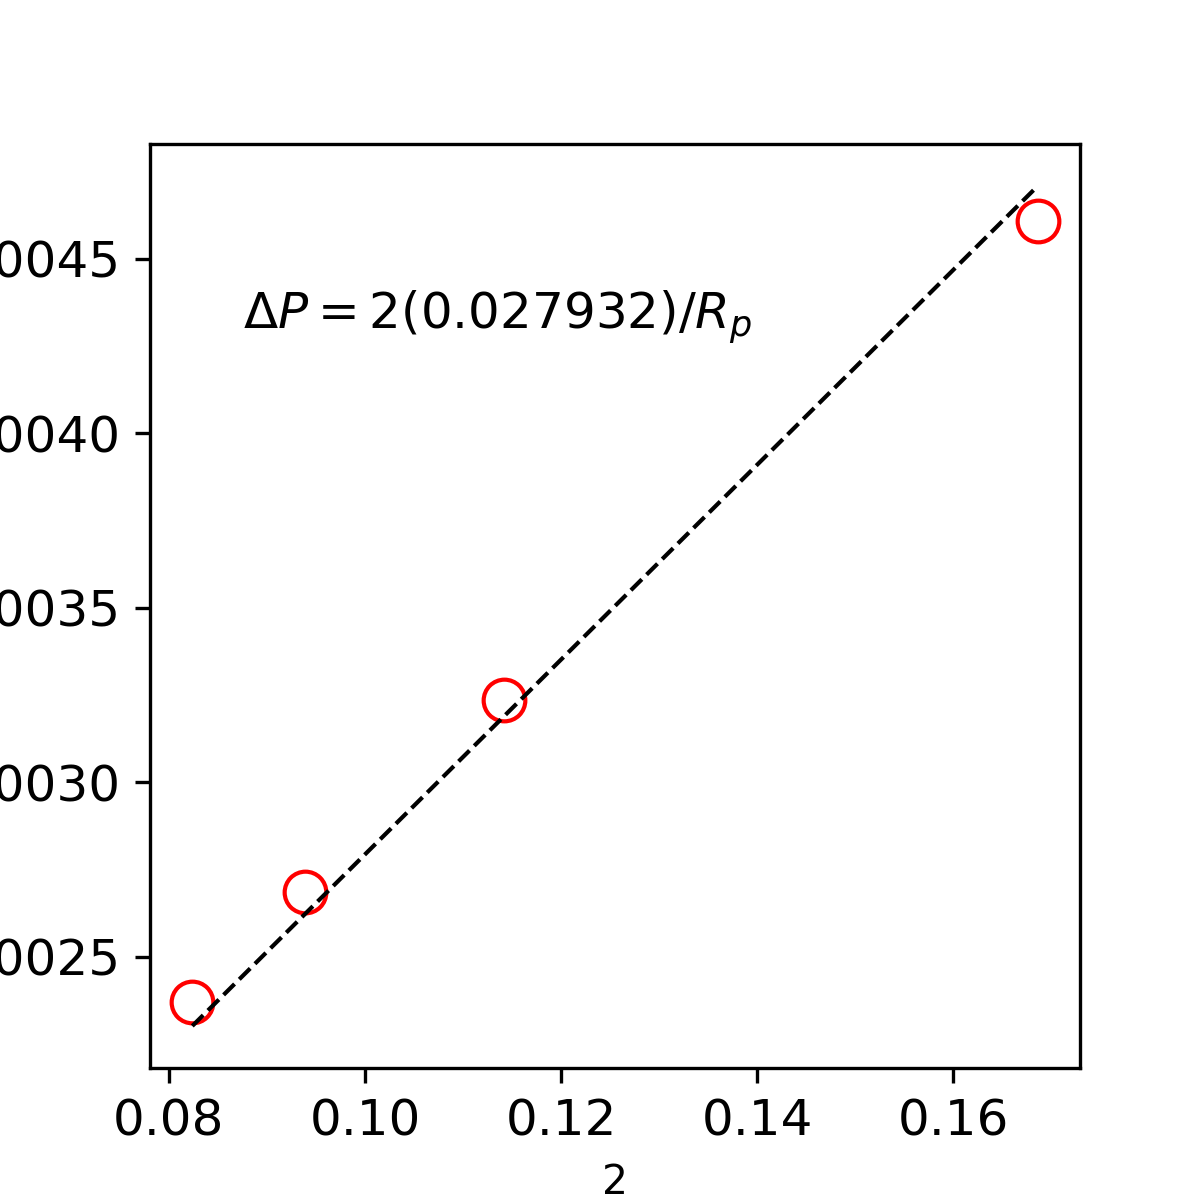
\includegraphics[scale = 0.5]{figures/model_validation/surface_tension.png}
    \caption{Plot of the surface tension of the multicomponent model in this work calculated using the 
    Young-Laplace equation.}
    \label{fig:young_laplace_valid}
\end{figure}

Using the fluid and non-ideal mixing parameters defined in Table \ref{table:model_params}, a single water in oil 
droplet, termed blue in red, was initialized in the center system and run till the droplet radii reached steady state. 
This process was repeated for various droplet diameters, specified between $40$ and $85 \%$ of the system size at $5\%$ 
increments. The system had a box length of $L = 64$ and was run for $50000$ timesteps with periodic boundary conditions 
on all sides. Data was dumped every 10000 timesteps with only the last timestep used to calculate the values shown. Due 
to the diffuse interface present in this method, the density profiles were verified to be at steady state at the end of 
the simulation before further analysis was performed. \cite{frijters_effects_2012} Past work also showed that the 
pressures remained constant after 5 lattice units away from the interface. \cite{frijters_effects_2012} 

The pressure difference was calculated using the difference in scalar pressure between the center of the droplet and 
one of the corners of the box. Two techniques exist to calculate the radius of the droplet. The first directly measures 
the distance between opposite points of the droplet as measured from the density profile at opposite points of the droplet, 
and the second is based upon the total mass and density of the fluid making up the droplet. The second method offers greater 
accuracy by avoiding discretization errors that may exist in the first method, and also allows for the correction of 
particle volume at the interface if the system contained them. First, a local effective mass density 
$\rho^b_{eff} = \rho^{b}_{d} - \rho^{b}_{m}$ is found by calculating the difference in density between the blue 
fluid in the droplet and in the matrix. Next, the droplet mass is calculated as $M_d = \sum_{\mathbf{x}}{\rho_{eff}^{b}}$. 
The radius of the droplet can then be calculated from the mass and density of the droplets as $R_d = \sqrt[3]{\frac{3}{4\pi} 
\frac{M_d}{\rho^b_d - \rho^b_m}}$. To linearize the plot, the $\Delta P$ was plotted against $\frac{2}{R_d}$ with 
$\sigma$ being the slope of the fit.

Figure \ref{fig:young_laplace_valid} shows the results of the fit conducted of the Young-Laplace equation demonstrating 
that under these fluid and mixing parameters, the surface tension is $\sigma = 0.0279$. The fit was performed using 
\texttt{scipy.optimize.curve\_fit} with the fit function defined as $y = mx$. Droplets with starting sizes $2R_d < 70\%$ 
of the initial system size disappeared. This occurred due to the initial condition of each fluid set to not contain the 
other fluid species, meaning once the simulation was initiated diffusion of mass from the droplet to the bulk occurred, 
causing disappearance of the droplet until the thermodynamically optimal composition was reached. From the fit calculated 
in Figure \ref{fig:young_laplace_valid}, the fit is linear as long as the initial droplet size is sufficiently large. 
Alternatively, the composition of the system can be set to near equilibrium in order to allow access to smaller droplet 
sizes.

\subsection{Contact angle}
\label{section:model_contact_angle}

Contact angle plays a role in particle stabilized emulsions by controlling the free energy reduction that the interface 
has in addition to the imparting of preferential curvature. LB3D allows for modification of the contact angle of a 
particle through the addition of a shell of blue or red fluid to the surface of the Ladd particle termed as the particle 
color $(\Delta \rho)$. \cite{jansen_bijels_2011, gunther_lattice_2013} To ensure that the correct settings are used in 
these simulations, in addition to gaining understanding into how to change parameters if the need arises, the contact 
angle as a function of the particle color was calculated.

Experimentally and computationally, the contact angle can be calculated through direct measurement of the angle of a 
droplet on a substrate. A droplet that preferentially wets a substrate has a lower contact angle relative to that 
substrate material, physically manifesting as the droplet spreading on the substrate. At a liquid interface, the particle 
will prefer to be in the particle it wets more. Thus for a spherical particle, the contact angle can be calculated as 
$\theta_c = \arccos{\frac{h_p - h_i}{R_p}}$ where $h_p - h_i$ defines the distance between the center of the particle 
after reaching its steady state position and the interface and $R_p$ is the radius of the spherical particle. 
\cite{gunther_lattice_2013, davies_interface_2014} This has been extended to ellipsoidal particles through assuming 
that the particle will have its largest cross sectional area flat on the interface and using the radius that is 
perpendicular to the interface to calculate the contact angle, defined as $\theta_c = \arccos{\frac{h_p - h_i}{R_{\parallel}}}$ 
and $\theta_c = \arccos{\frac{h_p - h_i}{R_{\perp}}}$ if $\alpha < 1$ and $\alpha \geq 1$ respectively. 

The simulation was setup in a box of size $32\cdot32\cdot64$ with an interface lying at $z = 32$, and a single particle 
placed at the center of the box with periodic boundary conditions on all sides. Fluid and non-ideal mixing properties were 
the same as those listed in table \ref{table:model_params}. The particle was then placed at the center of the simulation 
box and run for $30000$ timesteps with data read every 500 timesteps. The contact angles shown are results from triplicate 
runs, and averages of the final 10 data points. 

\begin{figure}[h]
    \centering
    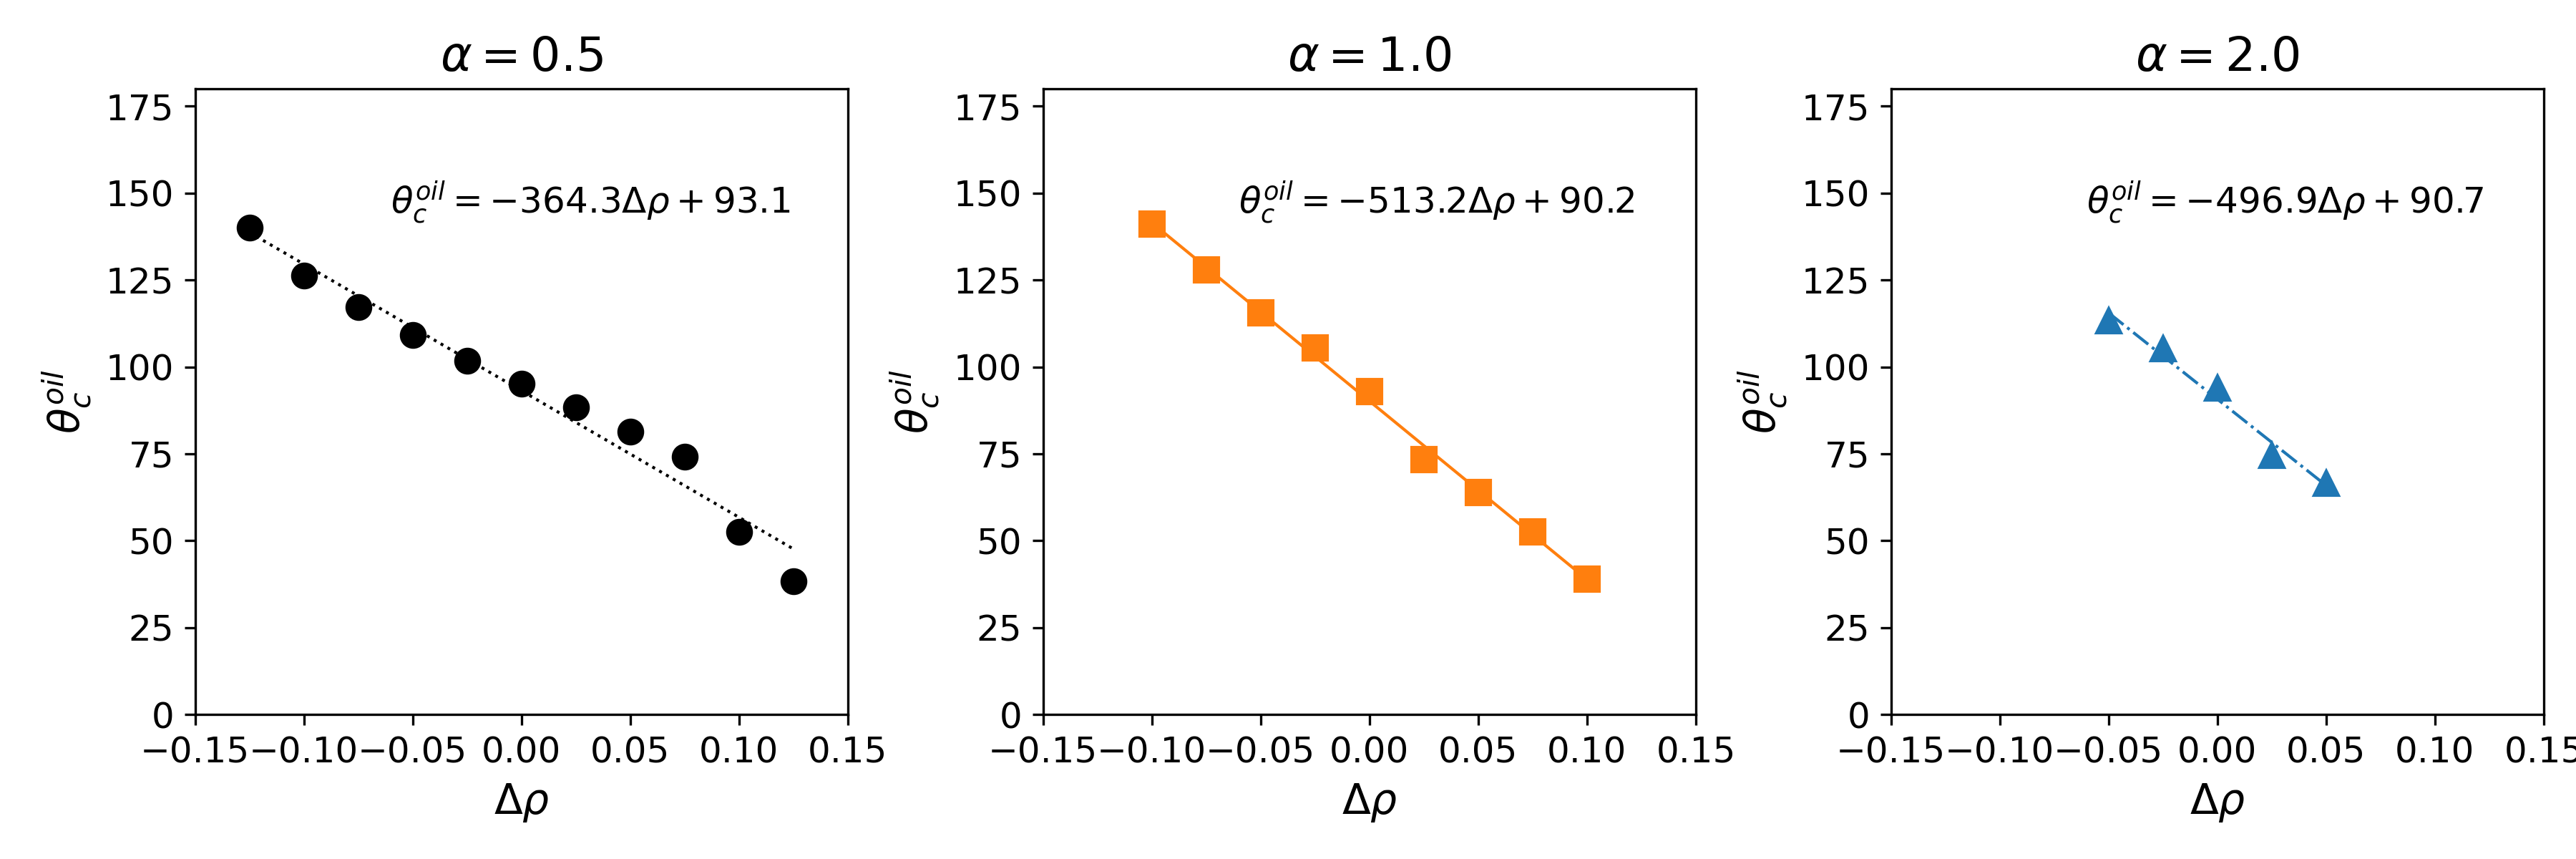
\includegraphics[scale = 0.5]{figures/model_validation/contact_angle_compare.png}
    \caption{Contact angle with respect to the oil phase, $(\theta_c^{oil})$ of the particles plotted against the 
    control parameter in LB3D}
    \label{fig:contact_angle_valid}
\end{figure}

Figure \ref{fig:contact_angle_valid} demonstrates the contact angles of the three particle geometries analyzed, 
confirming that $\Delta \rho = 0$ will result in neutrally wetting particles for all geometries. Oblate and spherical 
particles have usable particle colors between $-0.10 \leq \Delta \rho \leq 0.10$ while for prolate ellipsoids this 
value is $-0.05 \leq \Delta \rho \leq 0.05$. The slope of ellipsoidal particles appears to be lower which may arise 
from a larger interfacial adsorption energy, making it more difficult for surface energy changes to move particles out 
of the interface. At $\Delta \rho$ values further from 0, it was observed that the prolate particles tended to leave 
the interface rather than stay at a slightly off center equilibrium position. 

\section{Analysis techniques}

In this work, the structure factor derived domain size, geometric pore size distribution and tortuosity will be 
utilized to characterize the microstructure. The nematic order parameter will be used to characterize the particle 
order to the magnetic field. The average angle to the interface will be utilized to characterize how the particles 
ordering to the field affect the interface position. Finally, the radial distribution function will be used to probe 
how differences in ordering change the packing of particles on the interface. The time evolution of viscosity will 
provide insight into the rheological properties of the bijel, while the aforementioned analysis tools in addition to 
proportion of particles on the interface will be calculated to provide insight into how the bijel reacts to shear, 
parallel and perpendicular to the magnetic field. A more detailed description of the implementation of each method is 
shown in subsequent sections.

\subsection{Particle filling and interface smoothening}
\label{section:filling_routine}

Particles are the cause of bijels but they can also make characterization of domain size, curvature, pore size 
distribution and tortuosity more difficult as particles may change these parameters. An extrapolation scheme is 
required to connect the interface one different sides of the particles and to fill in the particles themselves so 
as to create a more accurate interface for other techniques.

This is accomplished through sequential density averaging and filling of grid points making up the particles from 
the outside in. The grid cells around a cell of interest are averaged using a D3Q19 like lattice and stepping through 
all points with a order parameter $\phi = \rho^w - \rho^o$ value of 0. 

\subsection{Domain size}
\label{section:domain_size}

The characteristic length scale at time $t$ of a bijel can be computed from the moments of the structure factor. The 
structure factor is first calculated from the order parameter of the phases, defined as $\phi = \rho_b - \rho_r$ where 
$\phi$ is the density order parameter and $\rho_b$ and $\rho_r$ are the densities of the blue and red fluid respectively. 
Next, the fluctuations of the order parameter $\phi'$ is calculated by subtracting the mean of the order parameter, 
$\langle \phi \rangle$ from the order parameter, defined as $\phi' = \phi - \langle \phi \rangle$. Next, the fourier 
transform of the fluctuations of the order parameter $\phi'(\mathbf{k})$ is calculated. Finally, $\phi'(\mathbf{k})$ 
is squared and made positive and normalized by the volume of the system defined as 
$S(\mathbf{k}) = \frac{1}{N} |\phi'(\mathbf{k})^2|$.

The first domain size metric used is the domain size derived from the spherically averaged first moment of the structure 
factor. The spherical averaging is done by averaging the values of the structure factor at the same $\mathbf{k}$ up 
till the nyquist frequency. The spherically averaged structure factor is defined as $S(k)$ where $k$ represents the 
wave numbers obtained from the spherical averaging. Next, the first moment $\langle k_1 \rangle$ is calculated as 
$\langle k_1 \rangle = \frac{\Sigma_{k} k\cdot S(k)}{\Sigma_{k} S(k)}$. Finally, the domain size is calculated as 
$L_1 = \frac{2 \pi}{\langle k_1 \rangle}$. \cite{kendon_inertial_2001,kendon_3d_1999} This domain size is used in past literature 
to calculate the correct scaling regime of a system undergoing spinodal decomposition. 

While it cannot be used to correlate physical phenomena the second moment of the structure factor derived domain 
size is utilized here to discriminate directional length scales. Owing to the spherical averaging done, the first 
moment moment derived domain size is unable to be used to calculate direction specific length scales. The second 
moment of the structure factor is first calculated by multiplying 
$\langle \mathbf{k_2}^2 \rangle = \frac{\Sigma_{\mathbf{k}} \mathbf{k}^2 S(\mathbf{k})}{\Sigma_k S(\mathbf{k})}$ 
where $\mathbf{k_2}^2$ represents the second moment in each cartesian direction. Next, the domain size in each 
direction is calculated as $L_2 = \frac{2 \pi}{\sqrt{\mathbf{k_2}^2}}$. \cite{jansen_bijels_2011, gunther_timescales_2014} 
In the rest of this document, $L_{\parallel}$ and $L_{\perp}$ is defined as the domain size parallel and perpendicular to 
the applied magnetic field.

\subsection{Curvature}
\label{section:curvature}

The simulation data was first pre-processed by calculating the order parameter of the densities, defined as the difference between the blue and red 
fluid densities at each grid point. $\phi(\vec{x}) = \rho^b(\vec{x}) - \rho^r(\vec{x})$. We then apply the particle filling algorithm described in 
section \ref{section:filling_routine} to the $\phi$ distribution, This reduces error from the presence of particles at the interface, 
resulting in an interface geometry that is more accurate to the bijel interface profile. From the filled order parameter, $\phi$, we calculate the mesh of 
the iso-surface representing the interface at $\phi = 0$ using a marching cubes method as implemented in scikit-image. We then use pyvista to calculate the 
gaussian and mean curvatures of the bijel microstructure, in addition to the interface area. The radii of curvature, $R_1, R_2$ are calculated from the 
mesh through measuring the angles between nearest neighbors and the laplacian of the faces to calculate the Gaussian and mean curvature respectively. 

We then limit the values of the calculated Gaussian and mean curvatures to reduce the effect of numerical artefacts created during the meshing process. We 
limit the Gaussian and mean curvatures to the expected curvatures around $|H| \approx \frac{2}{L}$ and $|K| \approx (\frac{2}{L})^2$. $L$ here is defined 
as the characteristic length scale obtained from the first moment of the spherically averaged structure factor described in section \ref{section:domain_size}.  
We then calculate an interface area normalized curvatures to remove the differences in absolute curvature values arising from the change in the characteristic 
length scale by calculating the surface area to volume ratio, $\Sigma = A_{int}/V$ where $A_{int}$ is the interfacial area and $V$ is the system volume. After 
dividing the obtained curvatures with $Sigma$, we obtain the discrete quantities, $H \Sigma^{-1}$ and $K \Sigma^{-2}$. For data presented as a time or magnetic 
field series, we sum each curvature distributions yielding, $\langle H \Sigma^{-1} \rangle$ and $\langle K \Sigma^{-2} \rangle$. For a bijel with volume ratio 
$50:50$ as used here, we expect $\langle K \Sigma^{-2} \rangle < 0$ and $\langle H \Sigma^{-1} \rangle \approx 0$.

\subsection{Tortuosity}
\label{section:tortuosity}

Tortuosity can be defined as the ratio between the path length $(L_{eff})$ of two points and the euclidean distance 
between two points $L_{0}$, $\tau = L_{eff}/L_{0}$. In practice this is the geometric definition of tortuosity as 
often the tortuosity of a system is dependent upon other factors. Diffusive tortuosity is what we will use here, 
defined as $\tau = \frac{D_{eff}}{D_0}$. This metric is also more relevant to the potential applications of bijels 
which rely on diffusion of mass for their uses.

Simulation techniques such as Lattice Boltzmann or Molecular Dynamics have been used to characterize the tortuosity of 
porous materials. However, these simulations can be computationally expensive and time consuming to perform, even though 
they may have great accuracy. Recently, particle diffusion techniques based on a random walk such as pytrax and taufactor 
or Pore Network Modelling (PNM) based techniques such as PoreSpy have been introduced which offer a tradeoff of accuracy 
for speed. Taufactor in particular is implemented on GPU's with a periodic boundary condition, allowing for rapid and 
accurate calculation of the tortuosity.

% \textcolor{blue}{https://joss.theoj.org/papers/10.21105/joss.05358, https://doi.org/10.1016/j.softx.2019.100277, https://joss.theoj.org/papers/10.21105/joss.01296}

Before using taufactor, the microstructure is first binarized. This is done by first calculating the order parameter of 
the system with $\phi = \rho_b - \rho_r$ where $\phi$ is the order parameter and $\rho_b, \rho_r$ are the densities of 
the blue and red fluid respectively. Next, the interface described with $\phi$ is smoothened using the algorithm detailed 
in section \ref{section:filling_routine}. \texttt{taufactor} determines the tortuosity by comparison
of steady-state diffusive flow through a porous medium with the bulk
diffusive flow in a control volume of the same size, molecular
diffusivity, and driving force \cite{cooper_taufactor_2016, kench_taufactor_2023}. We used
the \texttt{PeriodicSolver} to employ periodic boundary conditions. In many of the bijels synthesized using small molecule liquids, monomer is 
introduced into the oil phase and polymerized. Therefore, to perform the binarization step, we select all points where 
$\phi \leq 0$ and set their value to $0$, and all other values are set to $1$. To taufactor, $1$ represents void spaces 
and 0's are solid. \cite{cooper_taufactor_2016, kench_taufactor_2023}

\subsection{Interface order}
\label{section:interface_order}

We can calculate the ordering of the interface from the iso-surface of the interface. The simulation data was first pre-processed by calculating the 
order parameter of the densities, $\phi$. We then apply the particle filling algorithm described in section \ref{section:filling_routine} 
to the $\phi$ distribution. We then mesh the filled order parameter at $\phi = 0$ using the marching cubes algorithm and obtain the normals of the
vertices representing the points of the interface. We then computed the interfacial orientation tensor and plot that 
%
\begin{equation}
\tens{Q}_{\text{int}} = \frac{1}{\langle \mathrm{tr}(\tens{A}) \rangle} 
\left\langle \tens{A} - \frac{1}{3} \mathrm{tr}(\tens{A}) \mathsf{1} \right\rangle ,
\end{equation}
%
where the local tensor field $\tens{A}$ is defined by
%
\begin{equation}
\tens{A} = \nabla\phi\otimes\nabla\phi .
\end{equation}
%
The largest eigenvalue of $\tens{Q}$ is taken as the
interface nematic order parameter $S_{\text{int}}$.

\subsection{Channel size distribution}
\label{section:channel_size_distribution}

We use a method based on that outlined in Chan and Thornton. We create our distance function by performing an Eulerian Distance Transform on 
our order parameter data $\phi$ to obtain $\phi_{edt}$. \cite{chan_channel_2012} We smooth $\phi_{edt}$ using a boxcar algorithm with side length 3. 
We then normalize the distance from the interface in $\phi_{edt}$ using the characteristic length scale of the system defined as $\Sigma = \frac{V}{A_{int}}$
to obtain $\bar{\phi}_{edt}$ and a normalized distance from the interface, $\bar{r}$. A schematic of this workflow is demonstrated in Figure \ref{fig:csd_prep_viz}.

\begin{figure}
    \centering
    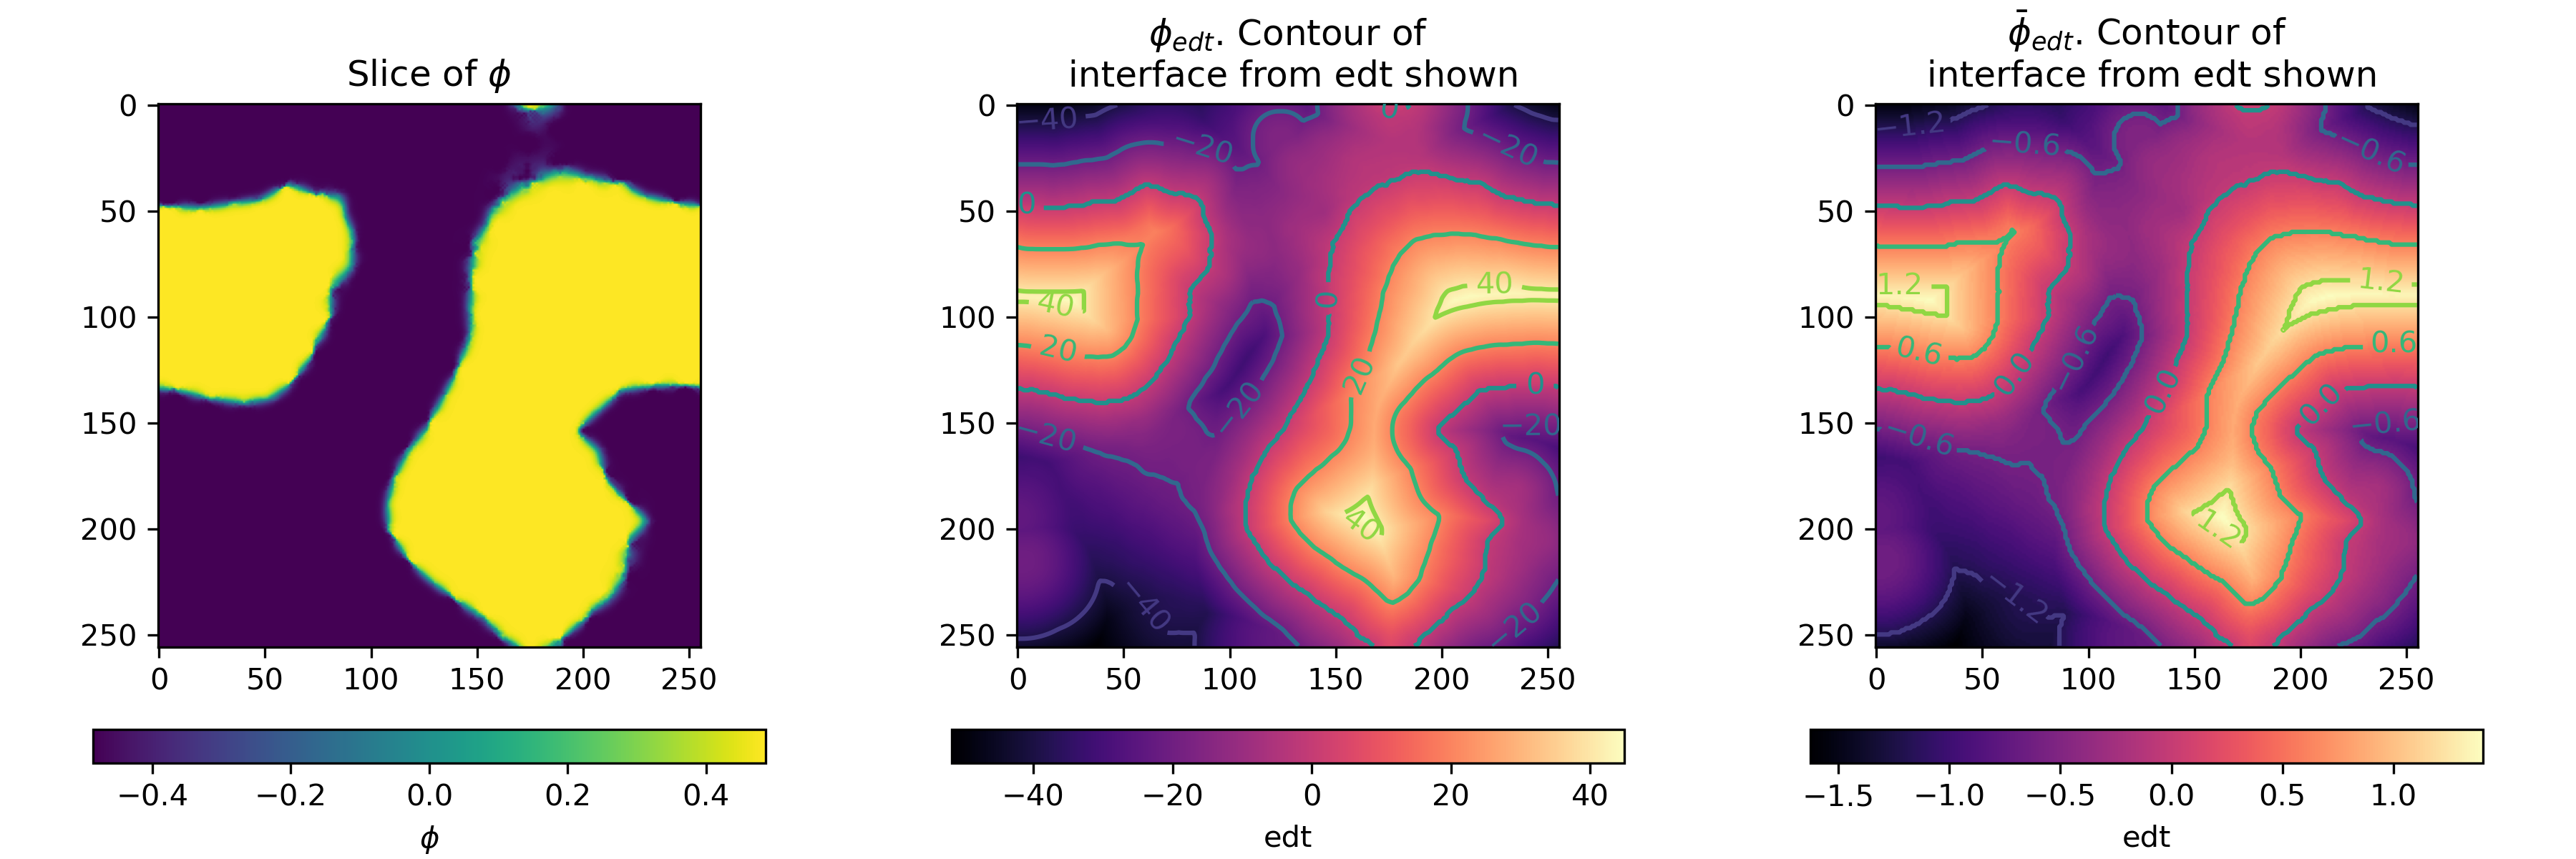
\includegraphics[scale = 0.4]{figures/analysis/csd_prep.png}
    \caption{Schematics detailing the order of operations of the steps to calculate the channel size distribution.}
    \label{fig:csd_prep_viz}
\end{figure}

The number of handles, $h$
in the iso-surface at different distances from the interface of $\bar{\phi}_{edt}$ is calculated. $h$ is also normalized by $\Sigma$ and the system volume
to obtain $\bar{h} = \frac{h}{V\Sigma^{-3}}$. The magnitude of the derivative of $\bar{h}$ with respect to $\bar{r}$, $f$, represents the channel size distribution.
A mean channel size can also be calculated from the first moment of the $f$.

\subsection{Nematic order parameter}
\label{section:nematic_order_parameter}

The orientational ordering of the particles to one another can be characterized using the nematic order parameter, 
defined as $S$. This parameter was first used to characterize liquid crystals. However its use has expanded to colloidal 
systems to characterize the ordering of a system to an average orientation, termed the director. A system is said to have 
nematic ordering if its components have orientational order to the director but does not require the system to have 
translational order.

The nematic order parameter is calculated from the orientational alignment tensor, $Q$, which is calculated from the 
orientation of particles to one another as 
$\langle Q \rangle = \frac{1}{N} \sum_{i}^{N} \langle \frac{3}{2}u_i u_i - \frac{1}{2}I \rangle$. $u_i$ is the 
orientation of particle $i$ and $I$ is an identity matrix. \cite{veerman_phase_1992} While there are multiple 
methods to evaluate the nematic order parameter, the one we have picked is where the largest eigenvector is $S$, 
with its corresponding eignvector referring to the director of the system. \cite{veerman_phase_1992} 
% \textcolor{blue}{https://doi.org/10.1080/00268978400101951} 
A system is defined to be ordered nematically, 
if $S > 0.3$. In this work, the direction of the director will be compared to the direction of the magnetic 
field. We utilize the implementation in Freud to calculate the nematic order parameter.

\subsection{Radial distribution function}
\label{section:radial_distribution}

The radial distribution function (RDF) is used to measure the normalized number density of particles around a 
reference particle as a function of distance. The normalization factor is the expected density of particles derived 
from an ideal gas. The general form of the equation to calculate the RDF is 
$g(r) = \frac{1}{\rho_{ideal}(r) 4\pi r^2} \int_{r}^{r+\Delta r} \delta(r_{i} - r_{j}) dr$ where $\rho_{ideal}(r)$ 
represents the density expected at distance r from a reference particle in an ideal gas, $\delta(r_{i} - r_{j})$ 
represents the number of particles within the bin $r + \Delta r$ and integrated to get a volumetric density. 
As implemented in a numerical method, the integral becomes a sum. After correcting for the periodic boundary 
condition using the minimum image convention, the RDF can be used to characterize periodic systems. We utilize 
the implementation in the software package Freud. \cite{ramasubramani_freud_2020}

\begin{equation}
    g(r) = \frac{n_p-1}{n_p} V \left\langle\delta\left(r-r_i\right)\right\rangle ,
\end{equation}

where \(n_p\) is the number of particles in the volume
\(V\), and \(\langle\cdot\rangle\) denotes an average over all
particles. The radial distribution function was calculated by binning
the distance between all particle pairs and normalizing the shells with
respect to the distribution \(4\pi \rho r^2 \mathrm{d}r\) of an ideal
gas. 

\subsection{Average interface angle and proportion of particles on the interface}
\label{section:interface_angle}

One way to differentiate between whether the particles pull the interface or whether the tilt of the particles at 
the interface causes changes to the jamming point is to characterize the average interface angle. The average interface 
angle $(\psi)$ is defined as the angle between the orientation of the axis of symmetry of the particle and the interface 
normal. The former mechanism would show little to no change in the interface angle, while the former mechanism should 
show large differences. The proportion of particles on the interface can also be calculated using this technique. 

The orientation of the particle is obtained from the output files from the simulation. The interface normal needs to 
be calculated from $\phi$. This is done by taking $\phi$ as calaculated from the red and blue fluid densities, then 
performing the particle fill routine described in section \ref{section:filling_routine}. Next, a mesh corresponding 
to the interface is obtained using a marching cubes algorithm at a countour level of 0 with a cube length of 4 lattice 
units, which corresponds to the thickness of the interface. \cite{van_der_walt_scikit-image:_2014} The 
position of the particle and its closest vertex is calculated. If this distance is larger than the first minimum in 
the radial distribution function, it is considered to be not on the interface and the next step is not performed. The 
vertex and corresponding normal closest to the position of a particle is used in the dot product, 
$\cos{\psi} = \frac{n_{int} \cdot o_{i}}{|n_{int}| |o_i|}$ where $n_{int}$ is the normal of the interface and $o_i$ 
is the orientation of particle i. After looping through all the particles, the average of $\psi$ and the number of 
particles in the interface is calculated.

\subsection{Steinhardt order parameter}
\label{section:steinhardt_order_parameter}

Another factor affected by the application of the magnetic field is the Steinhardt 6 fold order parameter, $Q6$, which characterized the local 
particle ordering. \cite{steinhardt_bond-orientational_1983} It has been used to characterize crystallization, glass transitions and crystal 
structures for colloidal and molecular crystals. We utilize the average across all particles on the interface, $\langle Q6 \rangle$ and track 
this parameter as a function of time. Past work has identified that local crystallization of colloidal crystals takes place at $\langle Q6 \rangle = 0.38$, 
and that $\langle Q6 \rangle^{HCP} = 0.485$. \cite{steinhardt_bond-orientational_1983, toxvaerd_role_2020, mickel_shortcomings_2013} We utilize a voronoi 
cell derived definition of the neighbor list of each particle, addressing some of the shortcomings highlighted in the original distance based definition. 
\cite{steinhardt_bond-orientational_1983, mickel_shortcomings_2013}. We first define a complex orientational vector, $q_{lm}$

\begin{equation}
q_{lm}(i) = \frac{1}{N_b(i)} \Sigma_{j = 1}^{N_b(i)} Y_{lm}(\vec{R}_{ij})
\end{equation}

Where $N_b$ is the number of nearest neighbors of particle $i$, $l$ is controls to the degree of spherical harmonic to be calculated, $m$ is an integer 
defined as $-l \leq m \leq l$ that defines which spherical harmonic is being calculated and $\vec{r}_{ij}$ is the distance between two particle centers. 
The neighbor list $N_b$ is usually defined by a cutoff distance from the center of particle $i$ to its nearest neighbors $j$. Steinhardt then defined a 
bond order parameter $q_l$ from $q_{lm}$ as

\begin{equation}
Q_{l}(i) = \sqrt{\frac{4 \pi}{2l + 1} \Sigma_{m = -l}^{l} |q_{lm}(i)|^2}
\end{equation}

In the literature, crystal structures can be distinguished from one another by plotting the distribution of two or more $Q_{l}$. 
\cite{lechner_accurate_2008, mickel_shortcomings_2013} Given that bijels form colloidal glasses, we only expect there to be
short range order which means conclusions made from this parameter can only be used to guide trends of order, not quantitative 
calculations of crystal structures.


\subsection{Shear stress}
\label{section:shear_viscosity}

In an incompressible fluid, the viscosity $(\eta)$ is defined as the ratio between the measured 
shear stress $(\sigma)$ and the applied strain rate $(\dot{\gamma})$, $\sigma = \eta \dot{\gamma}$. In rheological 
experiments, the viscosity is measured through a viscometer based on Couette or shear viscometry and Poiselle or 
pressure gradient viscometry. A Couette cell functions by applying a shear velocity to one or more walls, and measuring 
the shear stress response of the fluid. Common geometries for Couette cells include the cone and plate and concentric 
cylinder viscometers. In simulations, shear can be applied to walls of the simulation domain through either a shearing 
wall boundary condition or a Lees Edwards boundary condition. We select the Lees Edwards boundary condition as shearing 
results are unaffected by finite size effects and wall effects. Finite size effects are observed as a system size
dependent shear stress at the same shear rate. Wall effects can be seen as stick-slip effects of the particles or 
unphysical velocity gradients near the wall.

In a lattice boltzmann, the shear stress is measured as the sum of the equilibrium and nonequilibrium contributions.
\cite{kruger_shear_2009} These terms are defined as,

\begin{equation}
    \sigma_{\alpha \beta} = \sigma_{\alpha \beta}^{0} + \sigma_{\alpha \beta}^{1}
\end{equation}

This expression is obtained from the Chapman Enskog expansion of the lattice boltzmann method. The equilibrium and
non-equilibrium contributions of the stress are defined as

\begin{equation}
    \begin{split}
        \sigma_{\alpha \beta}^{0} &= \rho c_s^2 \delta_{\alpha \beta} + \rho u_{\alpha} u_{\beta} \\
        \sigma_{\alpha \beta}^{1} &= (1 - \frac{1}{2 \tau})\Sigma_{i} (f_{i} - f_{i}^{eq})c_{i \alpha}c_{i \beta} \\
    \end{split}
\end{equation}

In this work, a shear velocity is imparted in the z direction, across the x-axis. Therefore, the shear stress in the x 
and z directions, $\sigma_{xz}$, is measured. $\sigma_{xz}$ is output as calculated from the simulation for the entire 
domain after applying this equation to the system. 

% \subsection{Yield stress and zero shear rate viscosity}
% \label{section:yield_stress}

% The yield stress of bijels can be calculated using the flow curve, stress ramp or from oscillatory rheological techniques. 
% The flow curve method involves the steady application of shear, followed by measurements of the shear stress response of 
% the material. The plateau of the shear stress response is indicative of the steady state stress of the material. The stress ramp 
% method involves the application of a shear stress onto the material, followed by measurements of the strain rate. A 
% perfectly elastic material will have no strain rate, while a perfectly dissipative material will have high strain rate. 
% The yield stress is characterized as the point when a rapid increase in strain rate is observed. The yield stress from 
% oscillatory rheology is defined when the storage modulus is lower than the loss modulus. This work will utilize the flow 
% curve method.

% The shear viscosity calculated using the method detailed in Section \ref{section:shear_stress} will be plotted as a 
% function of applied shear rate. Rheological models such as the Herschel Buckley, Bingham Plastic or Carreu models can be 
% utilized to fit the shear viscosity as a function of shear rate to calculate the zero shear rate viscosity. In bijel 
% applications, this parameter gives insight into the material stability and processability.


% \subsection{Shear banding}
% \label{section:shear_banding}

% \textcolor{blue}{https://doi.org/10.1073/pnas.0812519106}

% \textcolor{blue}{https://doi.org/10.1103/PhysRevX.11.021017}

% \section{Expected and current results}

% \subsection{Fields applied during fabrication}

\chapter{Application of a constant magnetic field onto a forming bijel}

\section{Introduction}

This section is based on work published in the Royal Society of Chemistry's Soft Matter journal and
work submited to the American Institude of Physics, Physics of Fluids journal. \cite{karthikeyan_formation_2024} 
It is reproduced from Ref \cite{karthikeyan_formation_2024} with permission from the Royal Society of Chemistry and 
reproduced from submission number \#POF25-AR-DSFD2024-03180, with the permission of AIP Publishing.

The addition of microstructure control in bijels can be utilized to improve the performance of porous materials
or soft matter derived from their co-continuous, tortuous microstructure. The importance of microstructure control
allows an increase in the charge/discharge rate of batteries through reducing the material tortuosity, or improving the 
adhesion and growth rate of bone grafts. These properties are imparted during the fabrication step of the bijel. Anisotropic
particles adsorbed at interfaces induce shape-dependent capillary interactions that have distinct effects on the
microstructure of emulsions, resulting in migration or rotation of particles at interfaces, in addition to the addition of
distinct timescales of domain coarsening. \cite{loudet_capillary_2005, cavallaro_curvature-driven_2011, gunther_lattice_2013}

In bijels, ellipsoidal stabilizers have been demonstrates to result in additional timescales of domain coarsening 
at long timescales owing to particle re-orientation at the interface due to interparticle capillary interactions 
at long timescales. \cite{gunther_timescales_2014} In addition to possessing more timescales, property, bijels stabilized 
with rod-like particles have been shown to result in smaller characteristic length scales, owing to the particles having a
larger cross sectional area resulting in jamming occurring at larger interfacial areas. \cite{hijnen_bijels_2015} 

Magnetic response has been used in particle stabilized emulsions in the past, causing controlled emulsion failure and
on-demand droplet coalescence for encapsulation and cargo release applications. \cite{melle_pickering_2005, zhou_magnetic_2011}
Fields also enable self assembly through the control of interface deformation derived capillary forces.
\cite{morgan_understanding_2013,davies_interface_2014,davies_dipolar_2015} Magnetically responsive spherical particle 
stabilized bijels have thus far not yielded significant microstructural modifications. \cite{kim_bijels_2010} However, 
electric fields have been shown to cause percolating cylindrical domains in electrically responsive bijels. \cite{carmack_tuning_2018}
The electric field causes polar interactions between particles, which causes the formation of chains of particles that
also function as nucleation sites for phase separation. \cite{carmack_tuning_2018}

In this chapter, I investigate the effect of external magnetic fields on the formation of bijels stabilized by 
anisotropic magnetic particles. The microstructure of bijels stabilized with oblate, spherical and prolate particles, 
namely the characteristic length scale and tortuosity, will be assessed as a function of the applied magnetic field
strength. I also characterize the underlying mechanisms governing the observed behavior. 

% Anisotropic particles, when adsorbed at liquid interfaces, induce
% shape-dependent capillary interactions that can have a distinct effect
% on the microstructure of emulsions
% \cite{loudet_capillary_2005,loudet_self-assembled_2009}. For instance,
% Madivala et
% al.~\cite{madivala_exploiting_2009,madivala_self-assembly_2009} found
% that emulsion stability can be significantly enhanced by ellipsoidal
% particles. Additionally, capillary interactions can lead to direct
% assembly of anisotropic particles
% \cite{bowden_self-assembly_1997,lewandowski_orientation_2010,stebe_oriented_2009,botto_capillary_2012}.
% Ellipsoidal particles can rotate and migrate on curved surfaces
% \cite{cavallaro_curvature-driven_2011}, where the interface curvature
% acts as an external field that controls the orientation and placement
% of particles \cite{furst_directing_2011}. Anisotropic particles at
% fluid interfaces were considered in Monte Carlo simulations by Bresme
% et al. to test the accuracy of thermodynamic models for the free
% energy as a function of the particle-fluid interactions, particle
% size, and orientation
% \cite{bresme_orientational_2007,bresme_computer_2008}. Harting and
% co-workers \cite{gunther_lattice_2013,gunther_timescales_2014} have
% performed lattice Boltzmann simulations of anisotropic particles at
% liquid interfaces and in emulsions. They found that anisotropic
% particles affect the dynamics of emulsion formation by introducing two
% additional timescales associated with particle rotation. Following
% initial adsorption, particles rotate to align their larger
% cross-section with the interface. When jamming sets in, capillary
% interactions cause the particle to re-orient in the interface leading
% to prolonged coarsening at long timescales. Due to the larger aspect
% ratio, ellipsoidal particles can stabilize a larger interface area
% leading to smaller domain sizes. Hijnen et
% al.~\cite{hijnen_bijels_2015} experimentally realized bijels
% stabilized by colloidal rods and analyzed their effect on the
% interface and domain morphology. Their experiments confirmed that
% jamming occurs at lower interface separations than for spherical
% particles with the same volume fraction. Moreover, they observed that
% the overall structure remains isotropic and attributed this to the
% rapid jamming of the rods. Additionally, they found that some rods
% tilted out of the interface due to the compression induced by domain
% coarsening.

% Particle-stabilized emulsions can be made responsive to external
% magnetic fields by magnetic particles
% \cite{melle_pickering_2005,zhou_magnetic_2011}. An external field can
% then be used to control the stability of the emulsion
% \cite{melle_pickering_2005} and the self-assembly of particles
% \cite{dassanayake_structure_2000,leunissen_directing_2009}. The tendency
% of anisotropic particles to adopt distinct orientations gives rise to an
% orientation transition when an external field is applied
% \cite{morgan_understanding_2012,davies_interface_2014,davies_dipolar_2015}.
% Magnetic fields thus offer a means to control the capillary interactions
% of ellipsoidal particles at an interface. For bijels stabilized by
% spherical magnetic particles, simulations by Kim et
% al.~\cite{kim_bijels_2010} revealed that magnetic fields do not have a
% significant effect on the microstructure of bijels. In contrast, Carmack
% and Millett \cite{carmack_tuning_2018} demonstrated that the structure
% of thin-film bijels stabilized by dielectric particles can change
% drastically when an external electric field is applied. The dielectric
% contrast of the particles induces polar interactions that cause liquid
% domain alignment leading to percolating cylindrical domains in the
% thin-film bijel. In addition, they found that particle chains can act as
% nucleation sites for phase separation. This suggests that anisotropic
% interactions can have a considerable effect on the phase separation and
% the resulting emulsion morphology and may offer a means to control the
% size and shape of liquid domains.

\section{Results}\label{sec:results_p1}

Bijels can be used as emulsion templates for porous materials with
applications including drug delivery, water desalination, and battery
electrodes
\cite{vanoli_bijels_2022, chen_pore-scale_2022, lu_controllable_2020, garcia_scalable_2019}.
The transport properties of porous materials depend on the porosity and
tortuosity of the void space and can be linked to the phase-separated
morphology of the bijel template. Therefore, I study the domain size
and tortuosity of the phase morphology of bijels stabilized by
anisotropic particles. In particular, I investigate the effect of
magnetic particles on the microstructure of bijels that are formed in
external magnetic fields. I simulated bijels with a particle volume
fraction of \(\phi_p=0.15\) and varied the magnetic flux density such
that the Bond numbers varies in the range \(0\le\bar{B}\le1\).
In this work, I use a fixed particle volume fraction and focus on the dependence of the 
bijel structure on the magnetic field. Bijels with varying particle loading and surface tension 
and have been studied elsewhere in the literature, e.g., by Hijnen et al.\cite{hijnen_bijels_2015} 
and Jansen and Harting\cite{jansen_bijels_2011}.

\begin{figure}
    \centering
    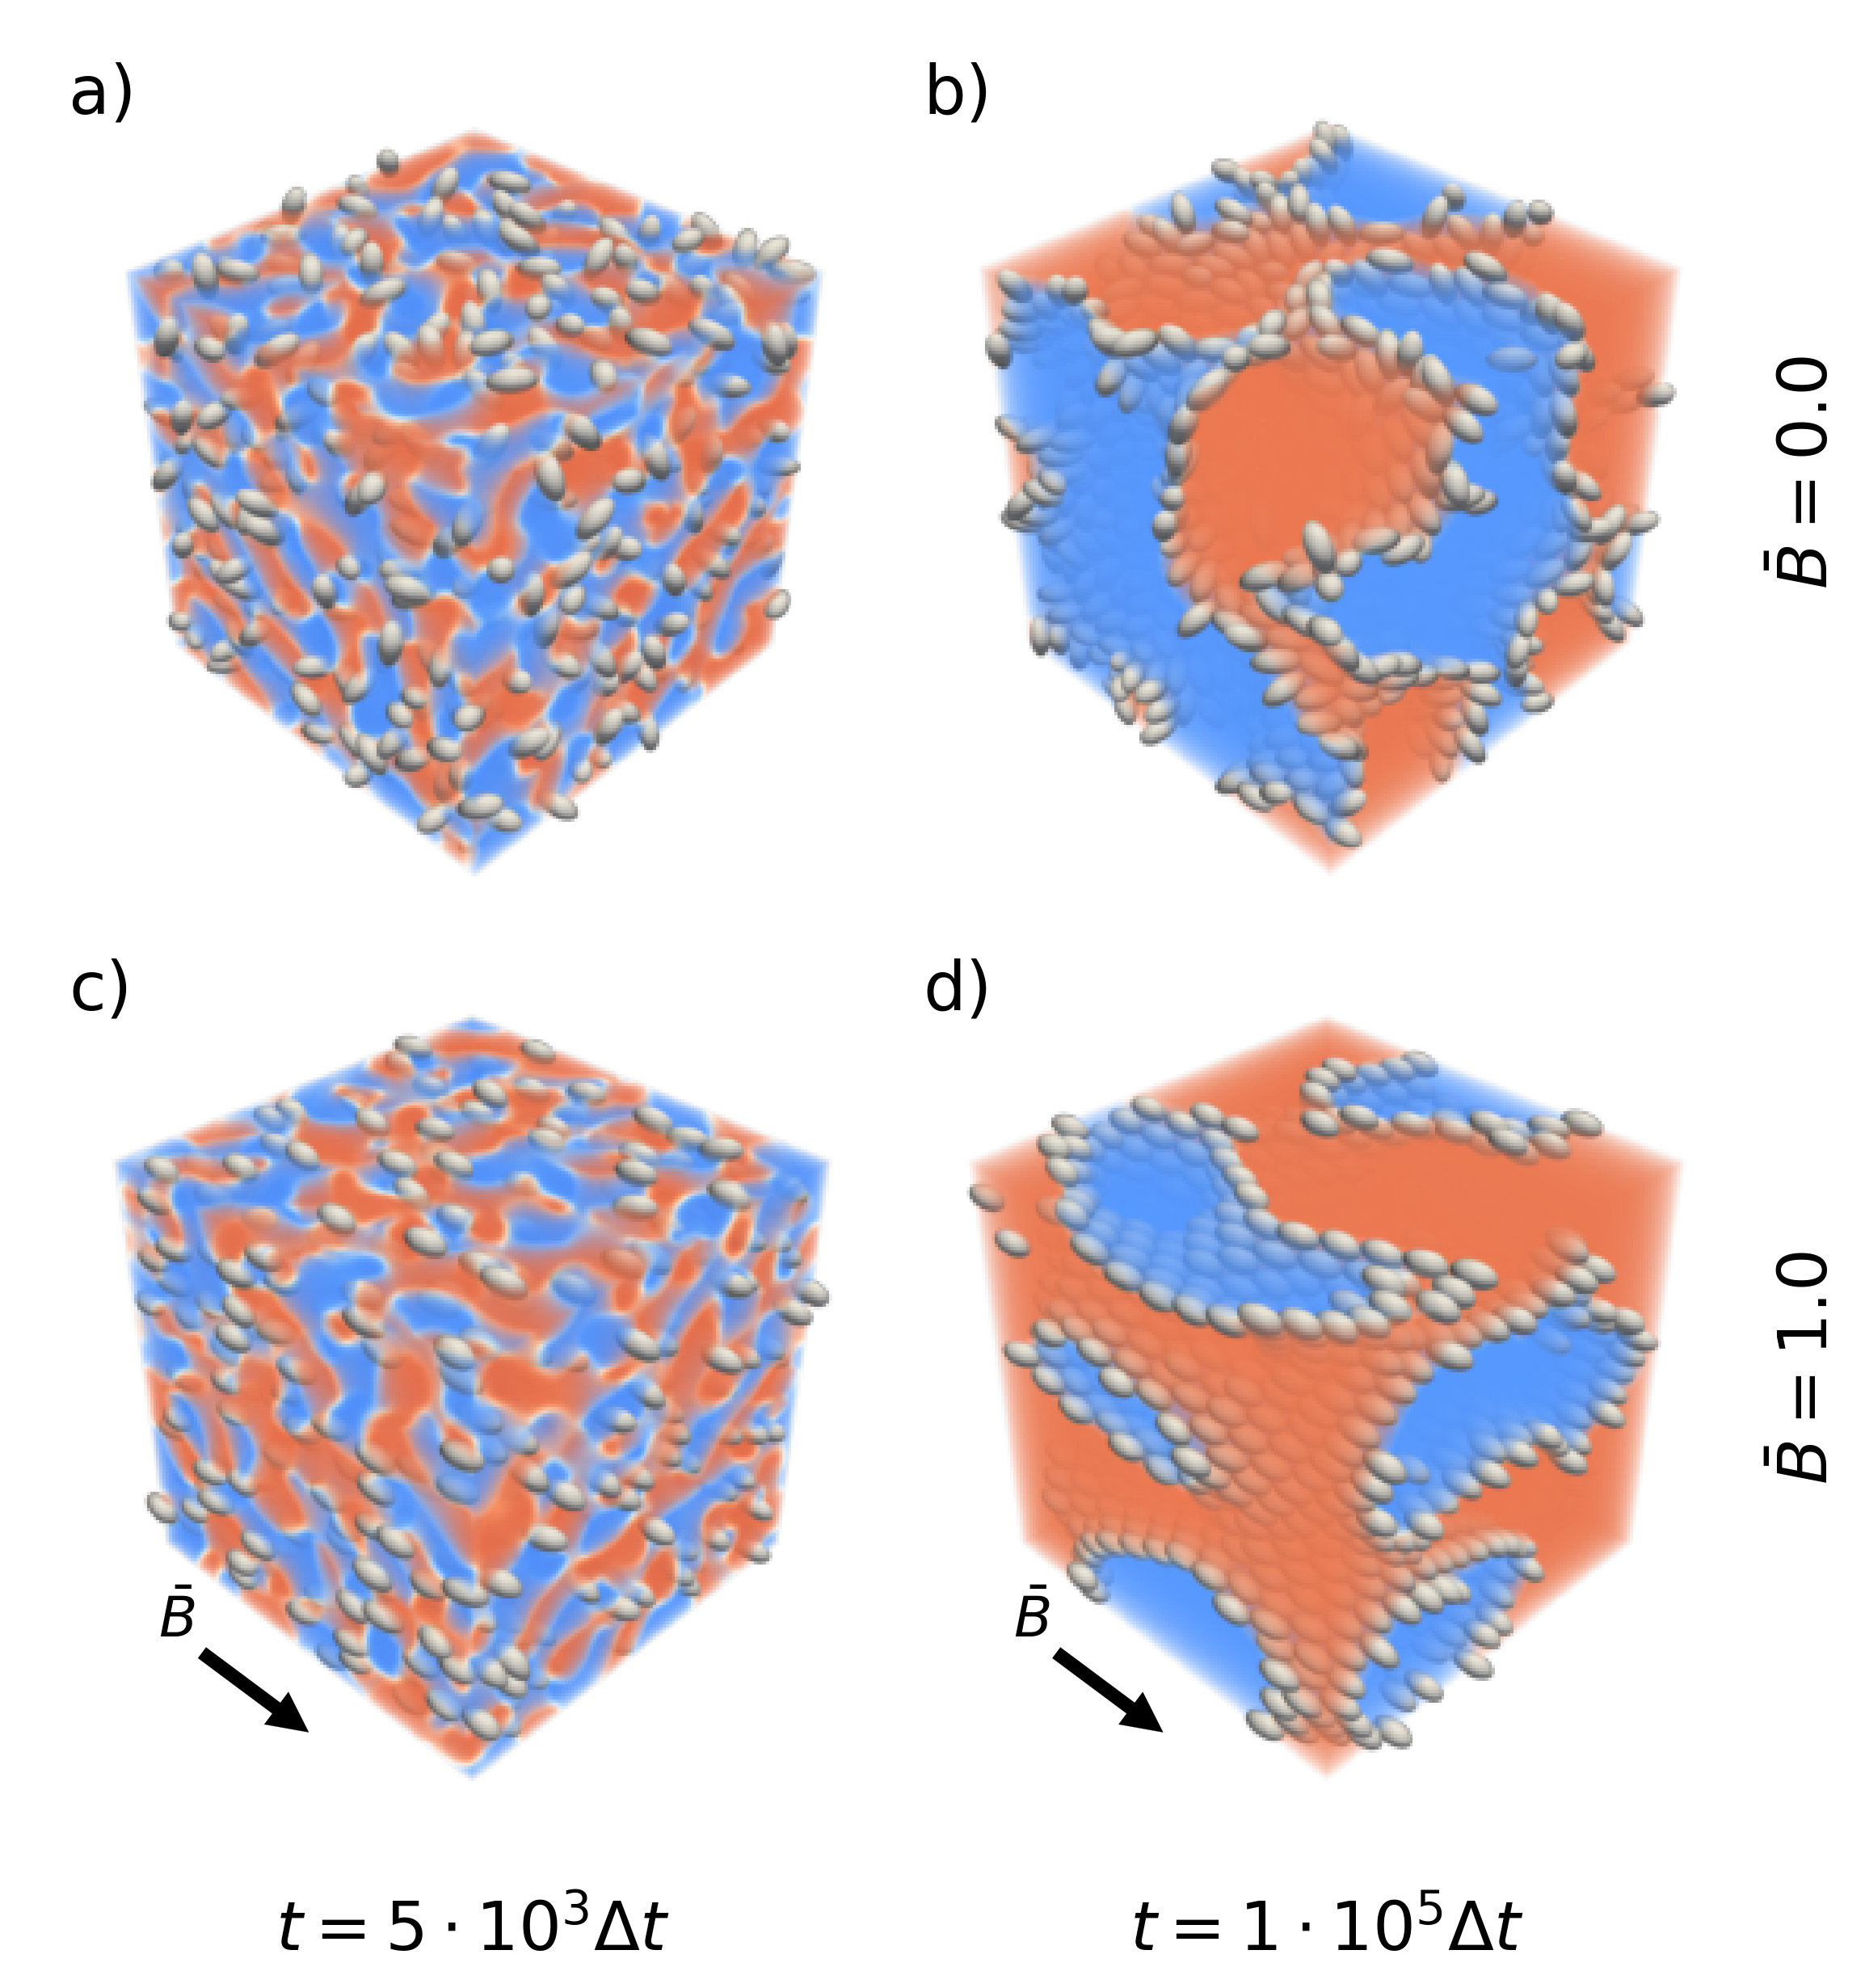
\includegraphics[width=0.5\columnwidth]{figures/results/paper1/microstructure_viz.png}
    \caption{Snapshots of emulsion gels stabilized by prolate ellipsoids after $t=5\cdot10^3$ timesteps (left) and after $10^5$ timesteps (right). The top row shows the structure forming without a magnetic field. 
             The bottom row shows the structure forming in an applied magnetic field of reduced strength $\bar{B}=1.0$. The snapshots are colored according to the order parameter $\phi$.}
    \label{fig:microstructure_viz}
\end{figure}

Figure \ref{fig:microstructure_viz} shows snapshots of the bijel
microstructure observed at different times with and without an external
magnetic field. The figure illustrates how anisotropic particles align
with the direction of the magnetic field. As the particles reorient,
they can deform the interface which thus responds by rearrangements
including reorientation and domain coalescence or breakup. This results
in apparently larger domain sizes for bijel formation in magnetic
fields. The quantitative effect on the bijel morphology, and domain size
in particular, is analyzed in the following sections.

\subsection{Structure factor and domain size of magnetically responsive bijels}

In LB simulations of spinodal decomposition, a characteristic length
scale can be obtained from the structure factor, defined in Section \ref{section:domain_size}. \cite{kendon_3d_1999,kendon_inertial_2001} 
It is worth noting that this definition of average domain size does not necessarily yield values that coincide with the typical
domain size observed visually in snapshots such as those shown in Fig.~\ref{fig:microstructure_viz}. However, in a dynamic
scaling regime, different measures of domain size are expected to differ only by a constant ratio. I found that the commonly 
used measure \(L_1(t)\) tends to overestimate the observed domain size. Numerically, the calculation of the spherically 
averaged structure factor is subject to poor statistics in the low \(k\)-shells, where the average \(|\vec{k}|\) of the 
lattice sites differs from the nominal shell radius. Additionally, the measurement of \(L(t)\) in simulations with
periodic boundary conditions is subject to finite size effects. More importantly, in suspensions of anisotropic particles, 
I cannot expect that the structure factor is isotropic. Therefore, I also used the 3D structure factor to calculate a lateral domain 
size in each Cartesian direction from the second moments also defined in Section \ref{section:domain_size}. 
\cite{jansen_bijels_2011,gunther_timescales_2014} I add the additional processing calculating a parallel and perpendicular domain size
from the results in each cartesian direction, defining $L_{\parallel}=L_z$ and $L_{\perp} = \frac{L_x+L_y}{2}$ I plot the structure factor of the structures in
Figure \ref{fig:structure_factor}.

\begin{figure*}
    \centering
    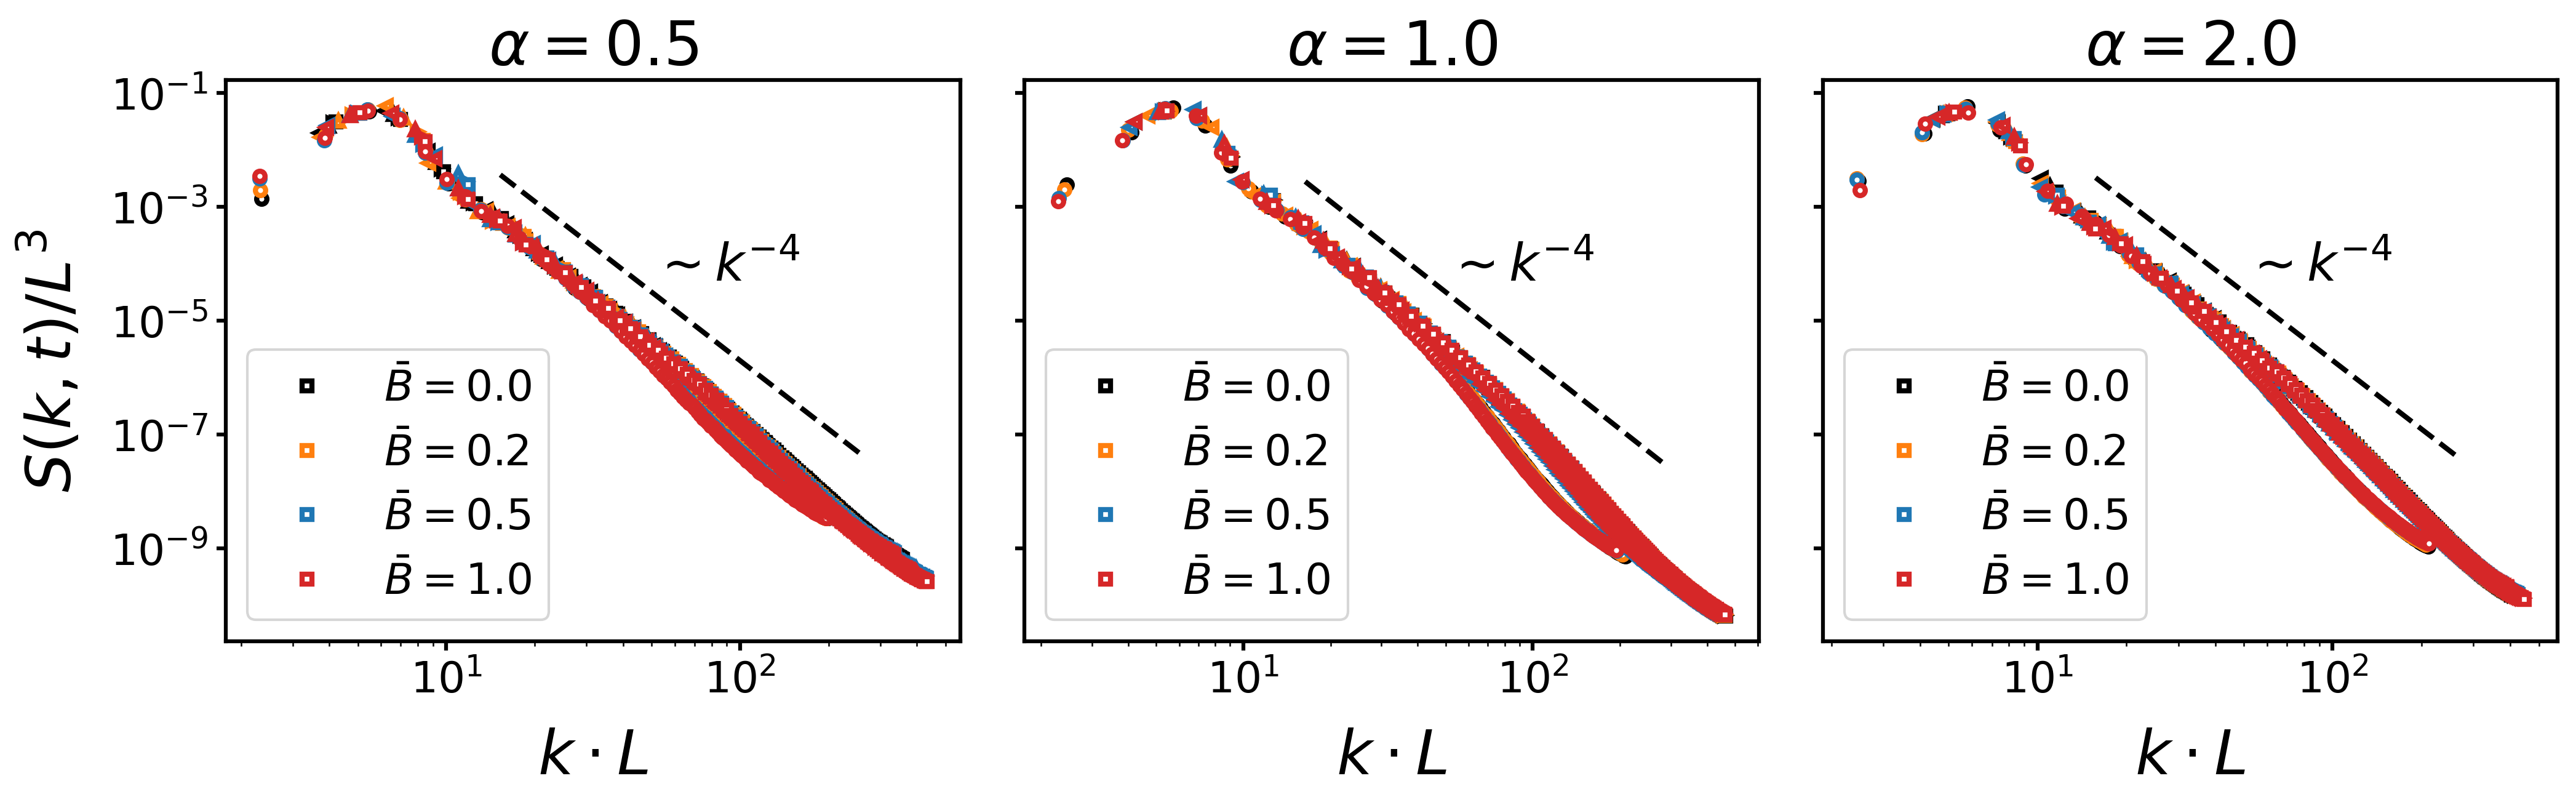
\includegraphics[width=\textwidth]{figures/results/paper1/structure_factor.png}
    \caption{Scaling plot of the dynamic structure factor $S(k,t)$ for different particle shapes $\alpha$ and at different 
            magnetic field strength $\bar{B}$. The structure factor is plotted at four different timesteps for each case. The good data collapse shows that the 
            bijel formation is driven by spinodal decomposition. The decay to the right of the peak is reasonably well described by Porod's law $S(k)\sim k^{-4}$.}
    \label{fig:structure_factor}
\end{figure*}

Figure \ref{fig:structure_factor} shows the scaling of the dynamic
structure factor \(S(k,t)\). The data collapse is good, albeit
deviations from dynamic scaling are present at smaller length scales.
The decay to the right of the maximum is reasonably well described by
Porod's law \(S(k)\sim k^{-4}\) indicating scattering off a nearly flat
interface. These results are in line with the scaling results by Kendon
et al.~\cite{kendon_3d_1999, kendon_inertial_2001} for spinodal
decomposition of binary fluids, which suggests that the formation of
bijels is primarily driven by the separation dynamics of the fluids. The
effect of the suspended particles only comes into play once larger
domains have formed and the coarsening interface reduces the accessible
area to the point where the particles start interacting. The onset of
particle interactions and subsequent jamming leads to a fairly sudden
slow-down of domain growth, as can be observed in the time evolution of
the domain size shown in Figure \ref{fig:domain_size}.

The domain size \(L_1\) obtained from the spherically averaged structure
factor initially shows a power law behavior very close to
\(L_1\sim t^{2/3}\). A nonlinear curve fit of the function
\(b(t-t_0)^a\) to the interval \(t\in[0,\ 3\cdot10^5\Delta x]\) yields
the exponents \(a=0.6448\) for spherical particles, \(a=0.6083\) for
oblate particles with aspect ratio \(\alpha=0.5\), and \(a=0.652\) for
prolate ellipsoids with aspect ratio \(\alpha=2\). These values are in
good agreement with the exponent \(a=2/3\) that is expected in an
inertial scaling regime, where the characteristic velocity \(U=dL/dt\)
scales with the characteristic length scale
\(U\sim \sqrt{\sigma/(\rho L)}\), leading to \(L \sim t^{2/3}\). After
around 30,000 to 40,000 time steps, the domain growth starts slowing
down and approaches a plateau at \(L_1\approx 200\Delta x\) for
spherical particles, \(L_1\approx 180\Delta x\) for the prolate
particles, and \(L_1\approx 170\Delta x\) for the oblate particles.
Interestingly, the alternative domain size measure \(L_d\) obtained from
the second moments of the 3D structure factor does not show the same
power law behavior. The rate of increase of \(L_d\) is substantially
smaller than that of \(L_1\), with a fitted exponent in the range of
0.12 to 0.20. The increase of \(L_d\) levels of earlier and reaches a
plateau around \(L_d\approx 70\Delta x\) for all three particle aspect
ratios. While dynamic scaling allows different measures of the
characteristic length scale to vary by a prefactor, the deviation from
the expected power law of both viscous and inertial scaling indicates
that the second moment of the 3D structure factor does not yield a
proper characteristic length scale. %, contrary to what has been assumed in
%previous works \cite{jansen_bijels_2011, gunther_timescales_2014}.
If one interprets the moments of the structure factor as moments of a
probability distribution, then the second moment of the 3D structure
factor is equivalent to the ratio of the fourth and second moments of
the spherically averaged structure factor (due to the factor \(k^2\) in
the volume integral). Hence \(L_d\) is perhaps better interpreted as
describing the shape of the structure factor (similar to kurtosis, but
not exactly the same) rather than a characteristic length scale.
Nevertheless, the second moments \(L_\beta\) provide separate measures
for the three Cartesian directions and can thus reveal anisotropy of the
domain morphology.

\begin{figure*}
\centering
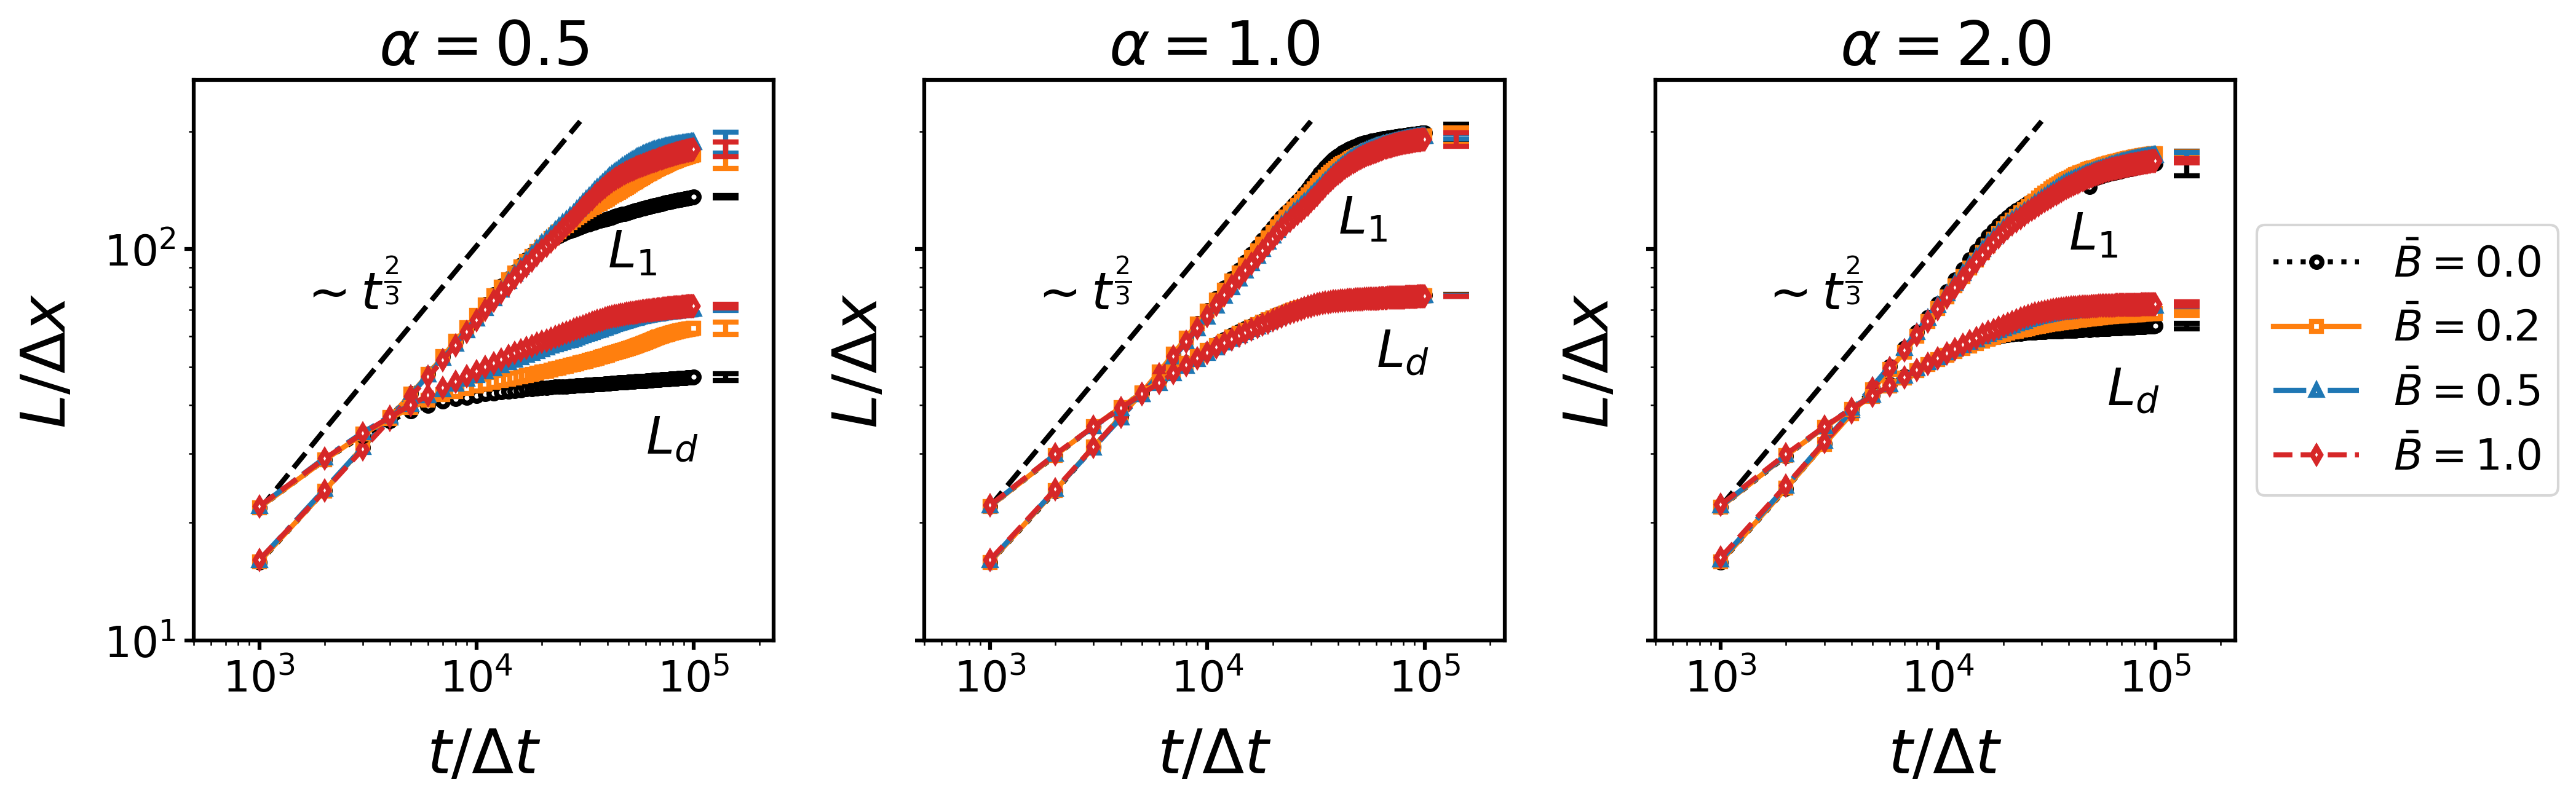
\includegraphics[width=\textwidth]{figures/results/paper1/domain_size.png}
\caption{Time dependence of the average domain size of the bijel for different particles shapes $\alpha$ and at different magnetic 
         field strength $\bar{B}$. $L_1$ denotes the domain size obtained from the first moment of the spherical average structure 
         factor, and $L_d$ denotes the domain size obtained from the second moment of the 3D structure factor. The increase roughly 
         follows a $\sim t^{2/3}$ scaling law indicative of the inertial regime of spinodal decomposition.}
\label{fig:domain_size}
\end{figure*}

\subsection{Effect of magnetic field on bijel formation}

\begin{figure}
\centering
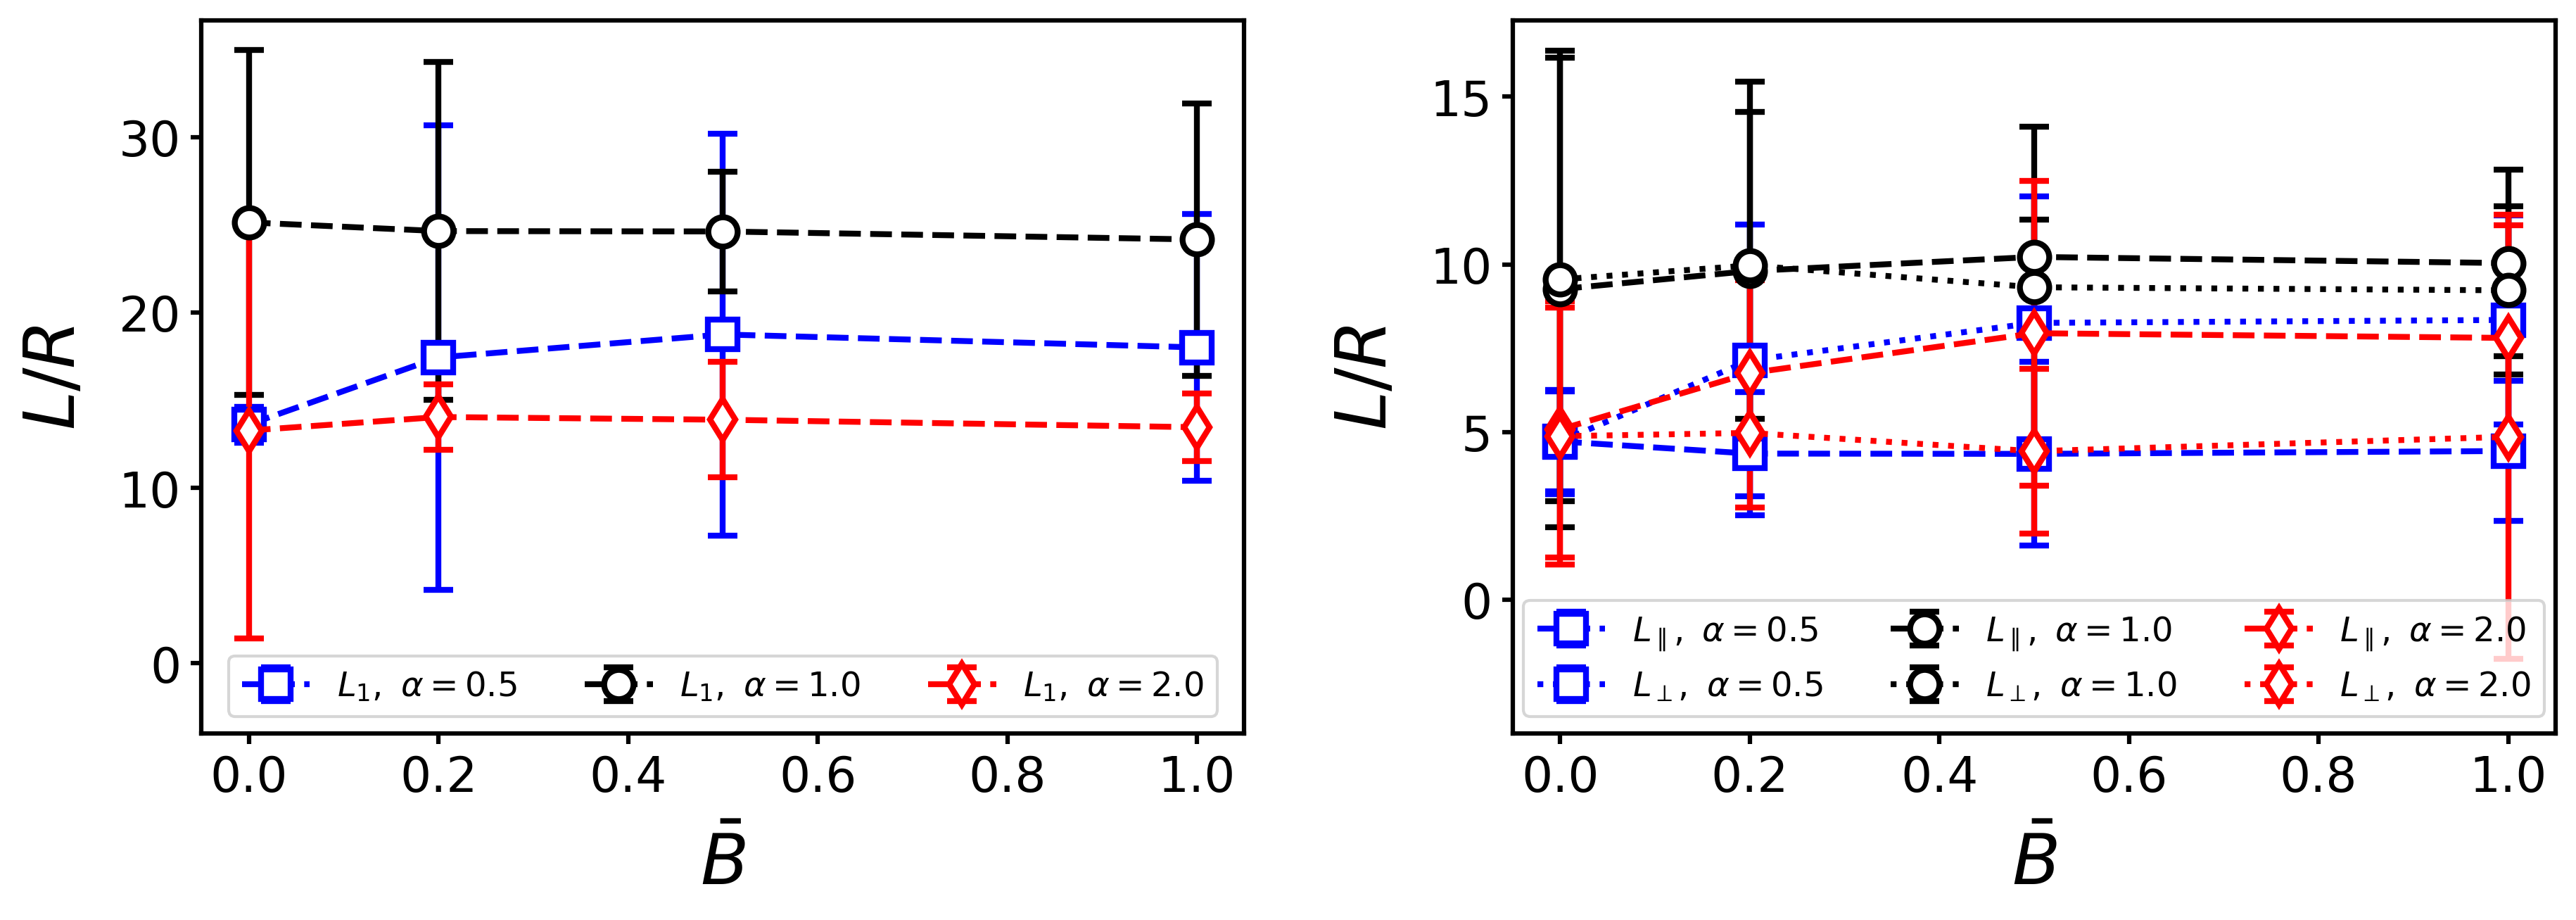
\includegraphics[scale = 0.4]{figures/results/paper1/D2a-vs-B_ss.png}
\caption{Dependence of the average domain size on the magnetic field strength $\bar{B}$. The left plot shows the average domain size $L_1$ obtained from the spherically averaged structure factor. The right plot shows the parallel and perpendicular domain size obtained from the respective second moments of the 3D structure factor. Errorbars indicate the standard deviation taken over three independent simulation runs. For anisotropic particles, the directional domain size becomes more anisotropic with increasing field strength.}
\label{fig:D2a_B}
\end{figure}

At first glance, the time-dependence of the domain size in Fig.
\ref{fig:domain_size} suggests that the domain size is not strongly
affected by the external magnetic field. In Fig.\ref{fig:D2a_B}a) I
plotted the domain size measure \(L_d\) normalized by \(R\), the larger
of the two radii of the ellipsoidal particles. The data points represent
the domain size measured at the final time step and averaged over three
independent simulation runs with the same parameters. The normalization
with the particle radius makes it apparent that the ellipsoidal
particles reduce the domain size of bijels. This observation is in line
with observations by Günther et al.~\cite{gunther_timescales_2014} and
indicates that -- relative to their volume -- ellipsoidal particles
stabilize a larger interface area than spherical particles. This is due
to the larger cross-sectional area of ellipsoidal particles at the same
volume. Furthermore, steric constraints prevent anisotropic particles to
pack less densely in the interface than spherical particles, as I will
discuss in more detail below.

The magnetic field does have an effect on the directional
domain size as shown in Figure \ref{fig:D2a_B} where I plotted the
domain size in the direction parallel and perpendicular to \(\vec{B}\)
separately. I find that for prolate particles, the domain size in the
parallel direction increases with the field strength up to approximately
three particle radii for the largest field, while the perpendicular
domain size stays constant. This trend is reversed for oblate particles
for which the domain size in the parallel direction decreases slightly
with field strength while the perpendicular domain size increases by
approximately four particle radii. Without a field, prolate
particles lead to smaller domain size than both spherical and oblate
particles, whereas they increase the domain size when the bijel forms under the
influence of a magnetic field. The anisotropy is due to the alignment of
ellipsoidal particles which leads to a closer packing within the
interface akin to nematic ordering. The difference between oblate and
prolate particles is caused by the orientation of the magnetic dipole
moment \(\vec{m}\) along the symmetry axis of the particles. In our
model, \(\vec{m}\) is aligned with the larger axis of prolate
ellipsoids, whereas it is aligned with the smaller axis of oblate
ellipsoids. Hence \(\vec{m}\) lies in the plane of the larger
cross-section of prolate particles while \(\vec{m}\) is perpendicular to
the larger cross-section of oblate particles. I thus expect that
alignment of the particles with the magnetic field \(\vec{B}\)
facilitates closer packing perpendicular to the field for prolate
particles, and parallel to the field for oblate particles. The
increase/decrease of domain size levels off at intermediate field
strength and further increases of the field have no additional effect.

\subsection{Tortuosity}

\begin{figure*}
\centering
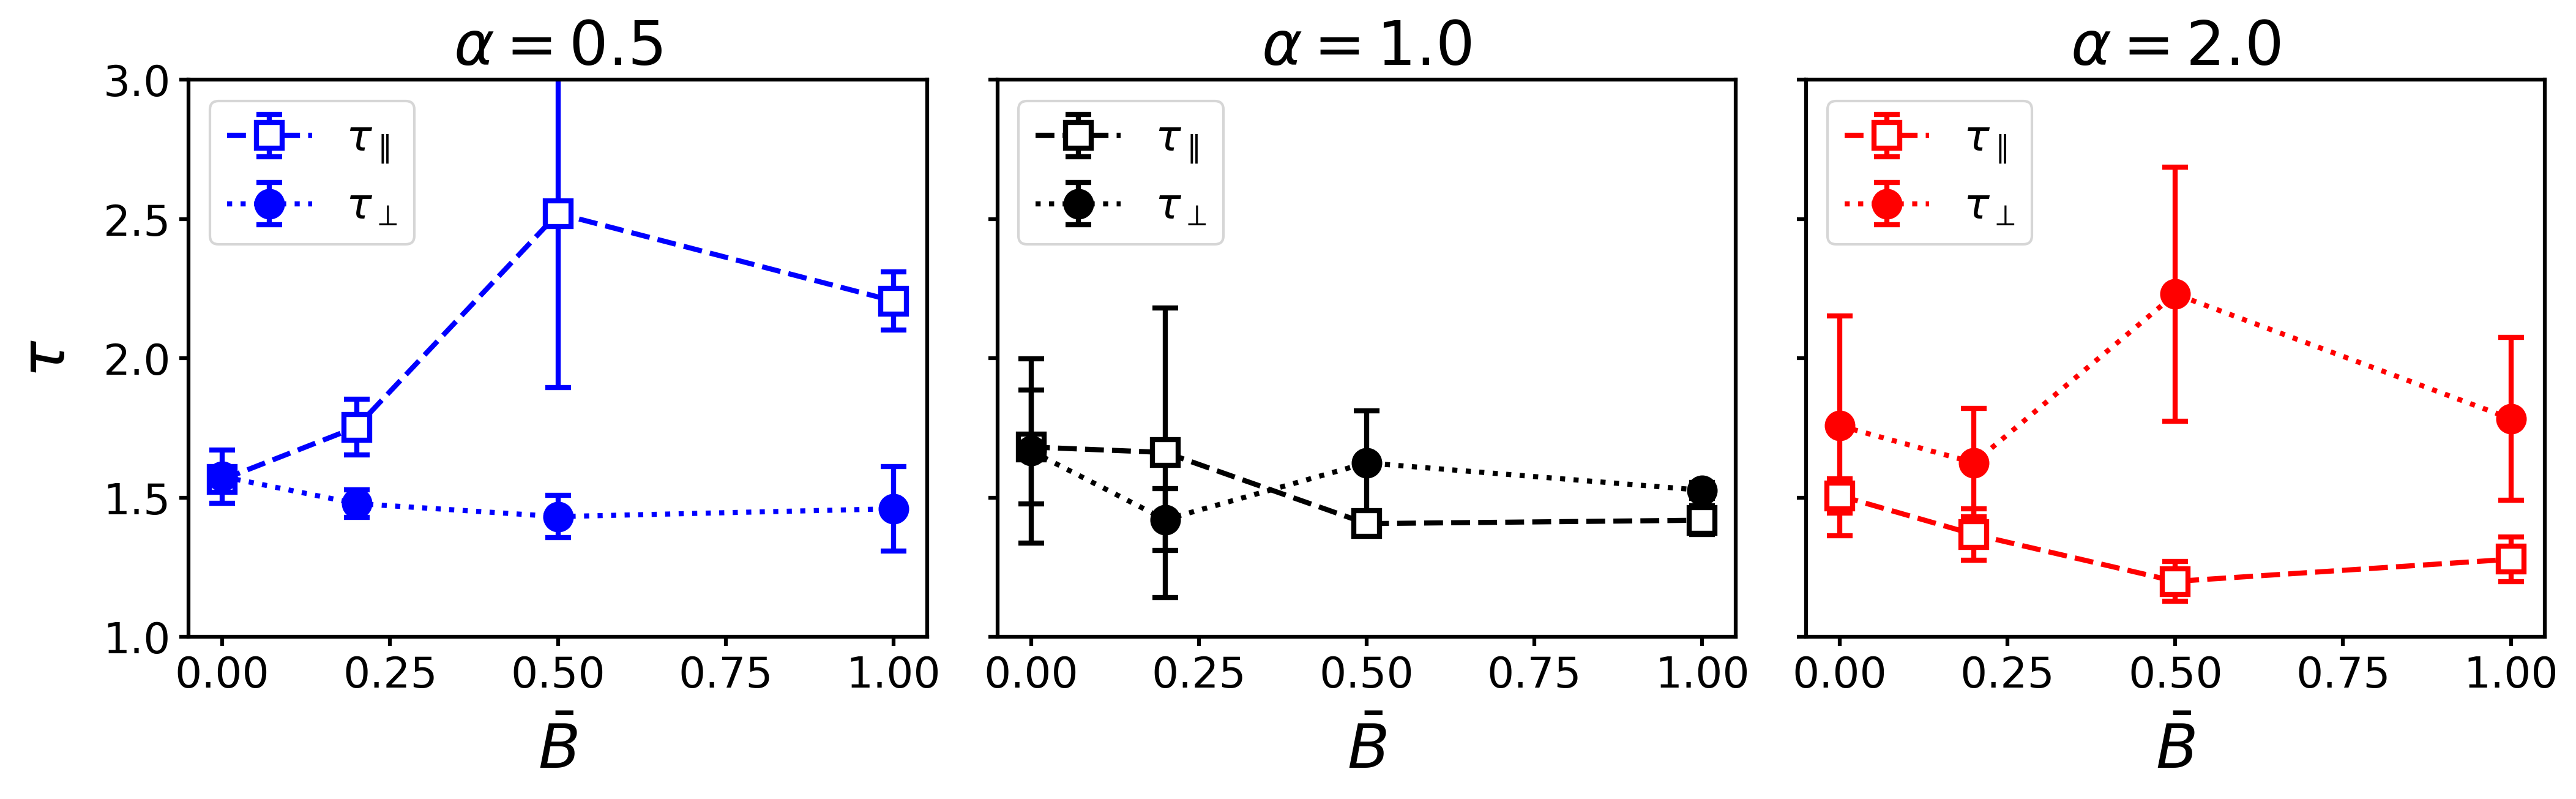
\includegraphics[scale = 0.4]{figures/results/paper1/tortuosity_compare.png}
\caption{Dependence of the tortuosity on the magnetic field strength $\bar{B}$ for different particle shapes $\alpha$. 
         Different components of the tortuosity tensor show the anisotropy for oblate and prolate particles.}
\label{fig:tau_B}
\end{figure*}

The anisotropy of domain size suggests that the magnetic field
influences the bijel morphology at the microscale. To investigate
whether these structural changes have an effect on macroscopic
transport properties, I also characterized the tortuosity of the
bijels. Various definitions of tortuosity have been proposed in the
literature \cite{dasilva_tortuosity_2022}, including geometric,
diffusional, and hydraulic tortuosity. Here I use the diffusional
tortuosity $\tau= \frac{\epsilon D}{D_{\text{eff}}}$, i.e., the ratio of the 
effective diffusivity $D_{\text{eff}}$ and the intrinsic diffusivity
$D$. I calculate the tortuosity using the procedure detailed in Section \ref{section:tortuosity}

Figure \ref{fig:tau_B} shows the results for the tortuosity as a
function of the applied magnetic flux for the three particle aspect
ratios. In the absence a magnetic field, the three aspect ratios lead to
a similar tortuosity around $\tau\approx 1.5$, slightly larger than
the tortuosity predicted by the Bruggeman relation
\(\tau=\epsilon^{-0.5}=1.41\) for equal volume fractions
\(\epsilon=0.5\) of the phases
\cite{bruggeman1935tortuosity, tjaden_origin_2016}. The observed
tortuosity is consistent with simulations of gyroid structures by Luo et
al., who found diffusive tortuosities in the range from 1.48 to 1.73
\cite{luo_macroscopic_2020}. Figure \ref{fig:tau_B} shows that in an
applied magnetic field, the tortuosity of bijels stabilized by
anisotropic particles (\(\alpha\neq1\)) becomes anisotropic as well.
Oblate particles (\(\alpha=0.5\)) lead to an increase of the tortuosity
\(\tau_\parallel\) in the direction of the magnetic field while the
tortuosity in the direction perpendicular to the magnetic field remains
around \(\tau_\parallel\approx1.5\). Conversely, prolate particles
(\(\alpha=2\)) lead to an increase of the tortuosity in the direction
perpendicular to the magnetic field, while the tortuosity in the
parallel direction slightly decreases with increasing field strength. In
both cases, the changes in tortuosity are consistent with the
anisotropic domain size and the alignment of particles with the magnetic
field. For prolate particles, the longer axis is aligned with the
magnetic moment and induces larger domain size and lower tortuosity in
this direction. The results show that the magnetic field has a
noticeable effect on the tortuosity of the bijel. I observe that the
largest change of tortuosity is measured at intermediate field strength
\(\bar{B}=0.5\). This suggests that the competition of interfacial and
magnetic forces and the resulting alignment of particles and liquid
domains induces morphological changes that are more complex than a
monotonic increase or decrease. I therefore turn to investigate the
microstructural changes within the bijel morphology in more detail.

\subsection{Curvature}

Beyond the length scale, curvature analysis offers insights into the
topological landscape of the bijel, facilitating further
microstructure optimization for various applications.
\cite{reeves_quantitative_2016} I plot the area averaged mean and
gaussian curvature \(H\Sigma^{-1}\) and \(K\Sigma^{-2}\) for bijels
stabilized with oblate, spherical and prolate ellipsoids at the final timestep in Figure
\ref{fig:curvature-vs-B_ss}. 

\begin{figure} 
    \centering 
    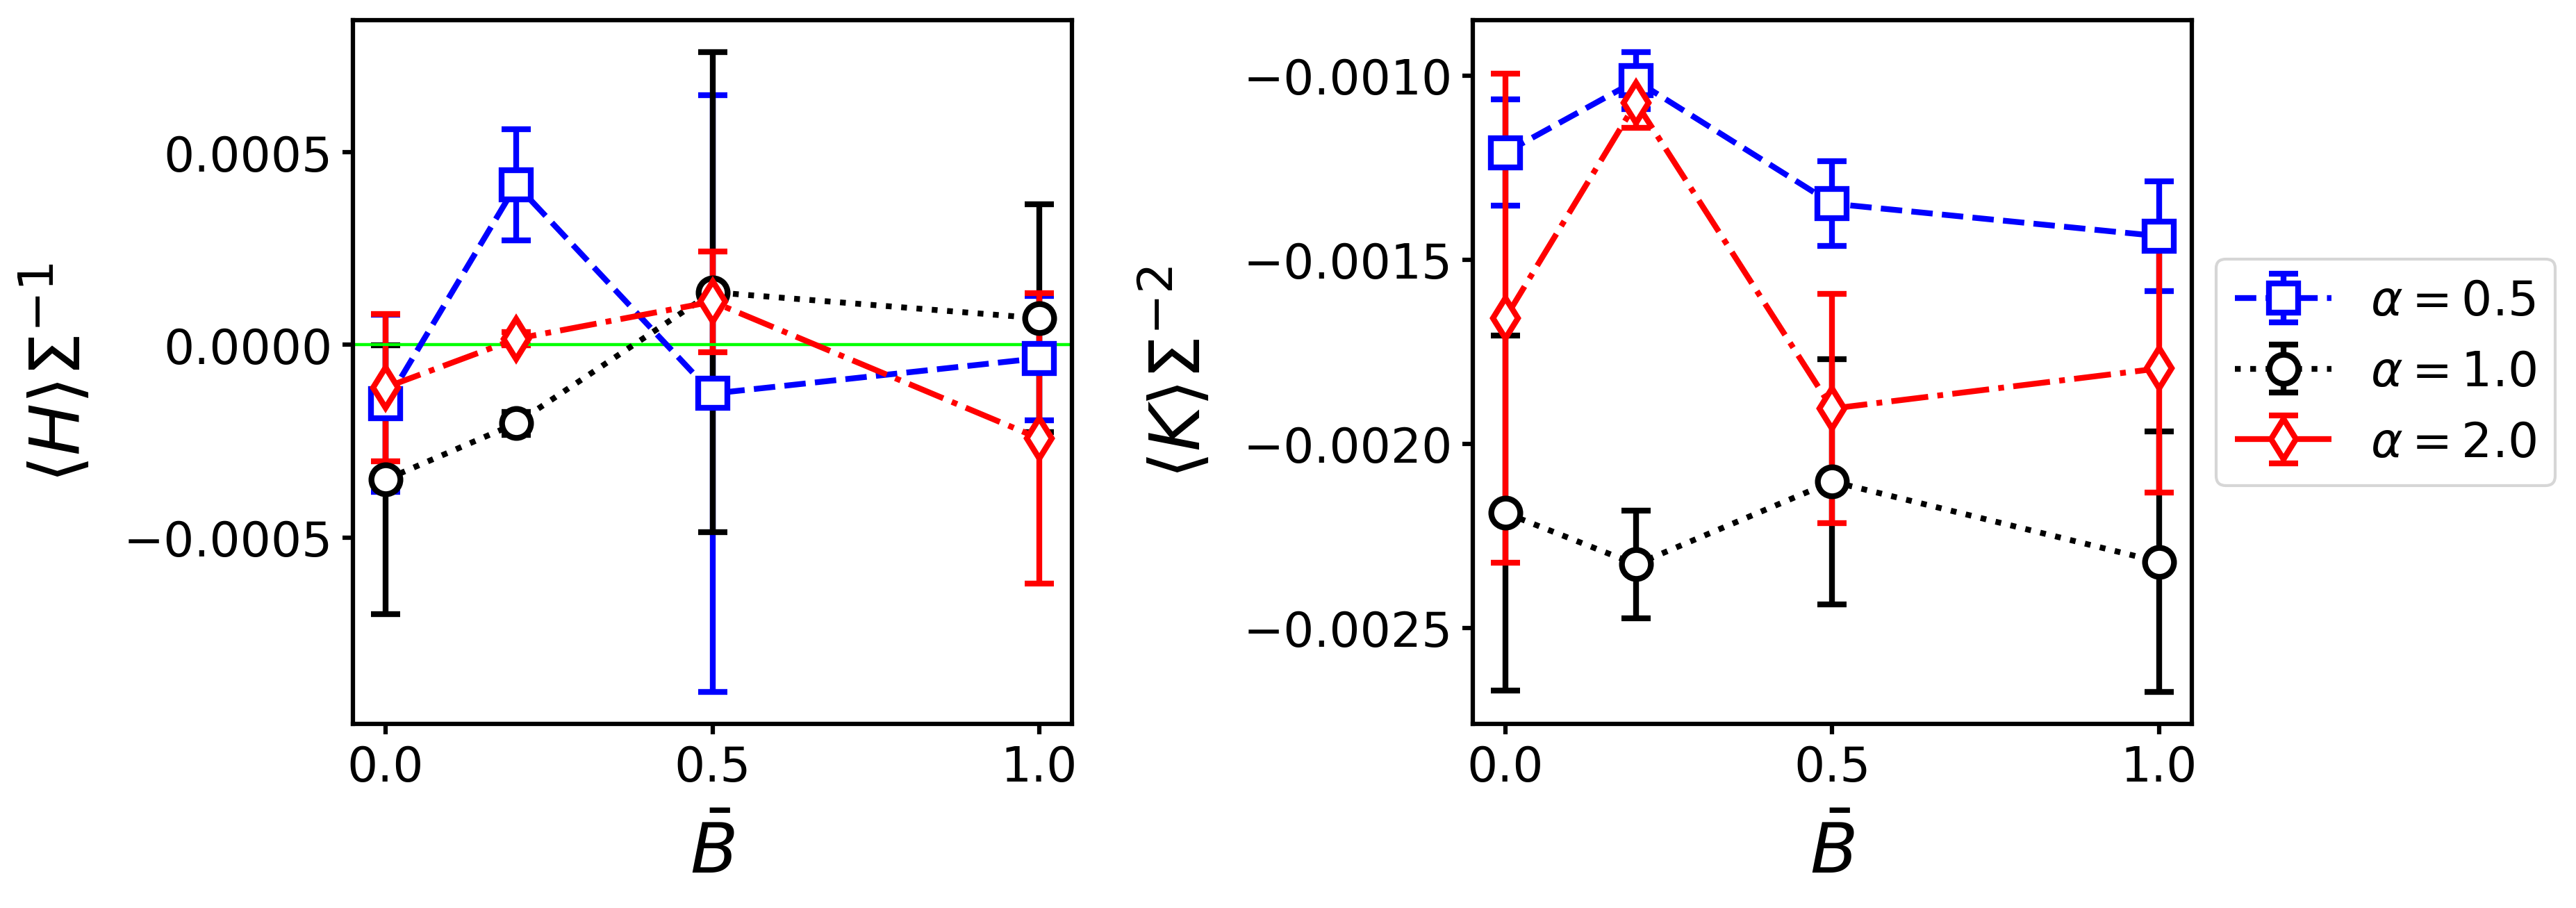
\includegraphics[scale = 0.4]{figures/results/paper1/curvature-vs-B_ss.png} 
    \caption{Plot of the area averaged mean $\langle H \rangle \Sigma^{-1}$ and Gaussian 
            $\langle K \rangle \Sigma^{-2}$ curvature in the left and right respectively. Each 
            plot contains the $\langle H \rangle \Sigma^{-1}$ and $\langle K \rangle \Sigma^{-1}$ 
            at the final timestep averaged across 3 runs for particles with $\alpha = 0.5, 1, 2$. 
            The mean curvature remains 0 on average, while the Gaussian 
            curvature shows a reduction as the magnetic field strength is increased for 
            ellipsoidal particles.} 
    \label{fig:curvature-vs-B_ss}
\end{figure}

Error bars are represented by the standard
deviation of the three simulations per parameter set performed. The area
averaged mean curvature shows little dependence on the applied field
strength with values around 0 and within error of one another. A value
near or at 0 is expected as the fluid volume fraction is equal and the
particles are neutrally wetting, implying the interface should not have
a preferred direction of curvature. \cite{jinnai_interfacial_2001} For
ellipsoidal particles, the gaussian curvature becomes more negative as
larger field strengths are applied. I also see that the gaussian
curvature becomes more positive as the interfacial area of the particle
increases. The trend of these results are inverse to the interfacial
area of each particle, \(A_{rm}\). This is expected behavior and is in
agreement with experiments that have investigated the effect of particle
size on the curvature of bijels. \cite{reeves_quantitative_2016}

To explain the reduction in $\langle K\Sigma^{-2} \rangle$ as a function of the applied field strength, two mechanisms are proposed. The first is that 
the particle alignment to the magnetic field during coarsening changes the topology of the surface, which upon jamming of ellipsoidal particles is locked in. 
The other proposed mechanism is that the time evolution of spinodal decomposition remains unaffected, but that the interface conforms to the magnetic field 
driven arrangement of particles upon jamming. While I cannot apply the Gauss Bonnet theorem to characterize the results, I can still relate the coarsening 
behavior of the bijel through its change in genus to the curvature. The time evolution of the genus serves as a topological technique to characterize the 
coarsening of the bijel, which alongside the $\langle K\Sigma^{-2} \rangle$, allows us to identify deviations from the coarsening behavior of bijels 
stabilized with spherical particles, and with magnetic fields. I calculate the genus by extracting the isosurface of the filled order parameter, where 
$\phi = 0$. It is then meshed using the marching cubes algorithm implemented in scikit-image with a cube size of 1. \cite{van2014scikit} From the vertices(v) 
and faces(f) generated from the marching cubes algorithm, I calculate the number of edges(e). The Euler Poincare characteristic, $\chi = n + f - e$. The genus is 
then obtained from the Euler Poincare parameter as $g = 1 - \chi/2$.

\begin{figure} 
    \centering 
    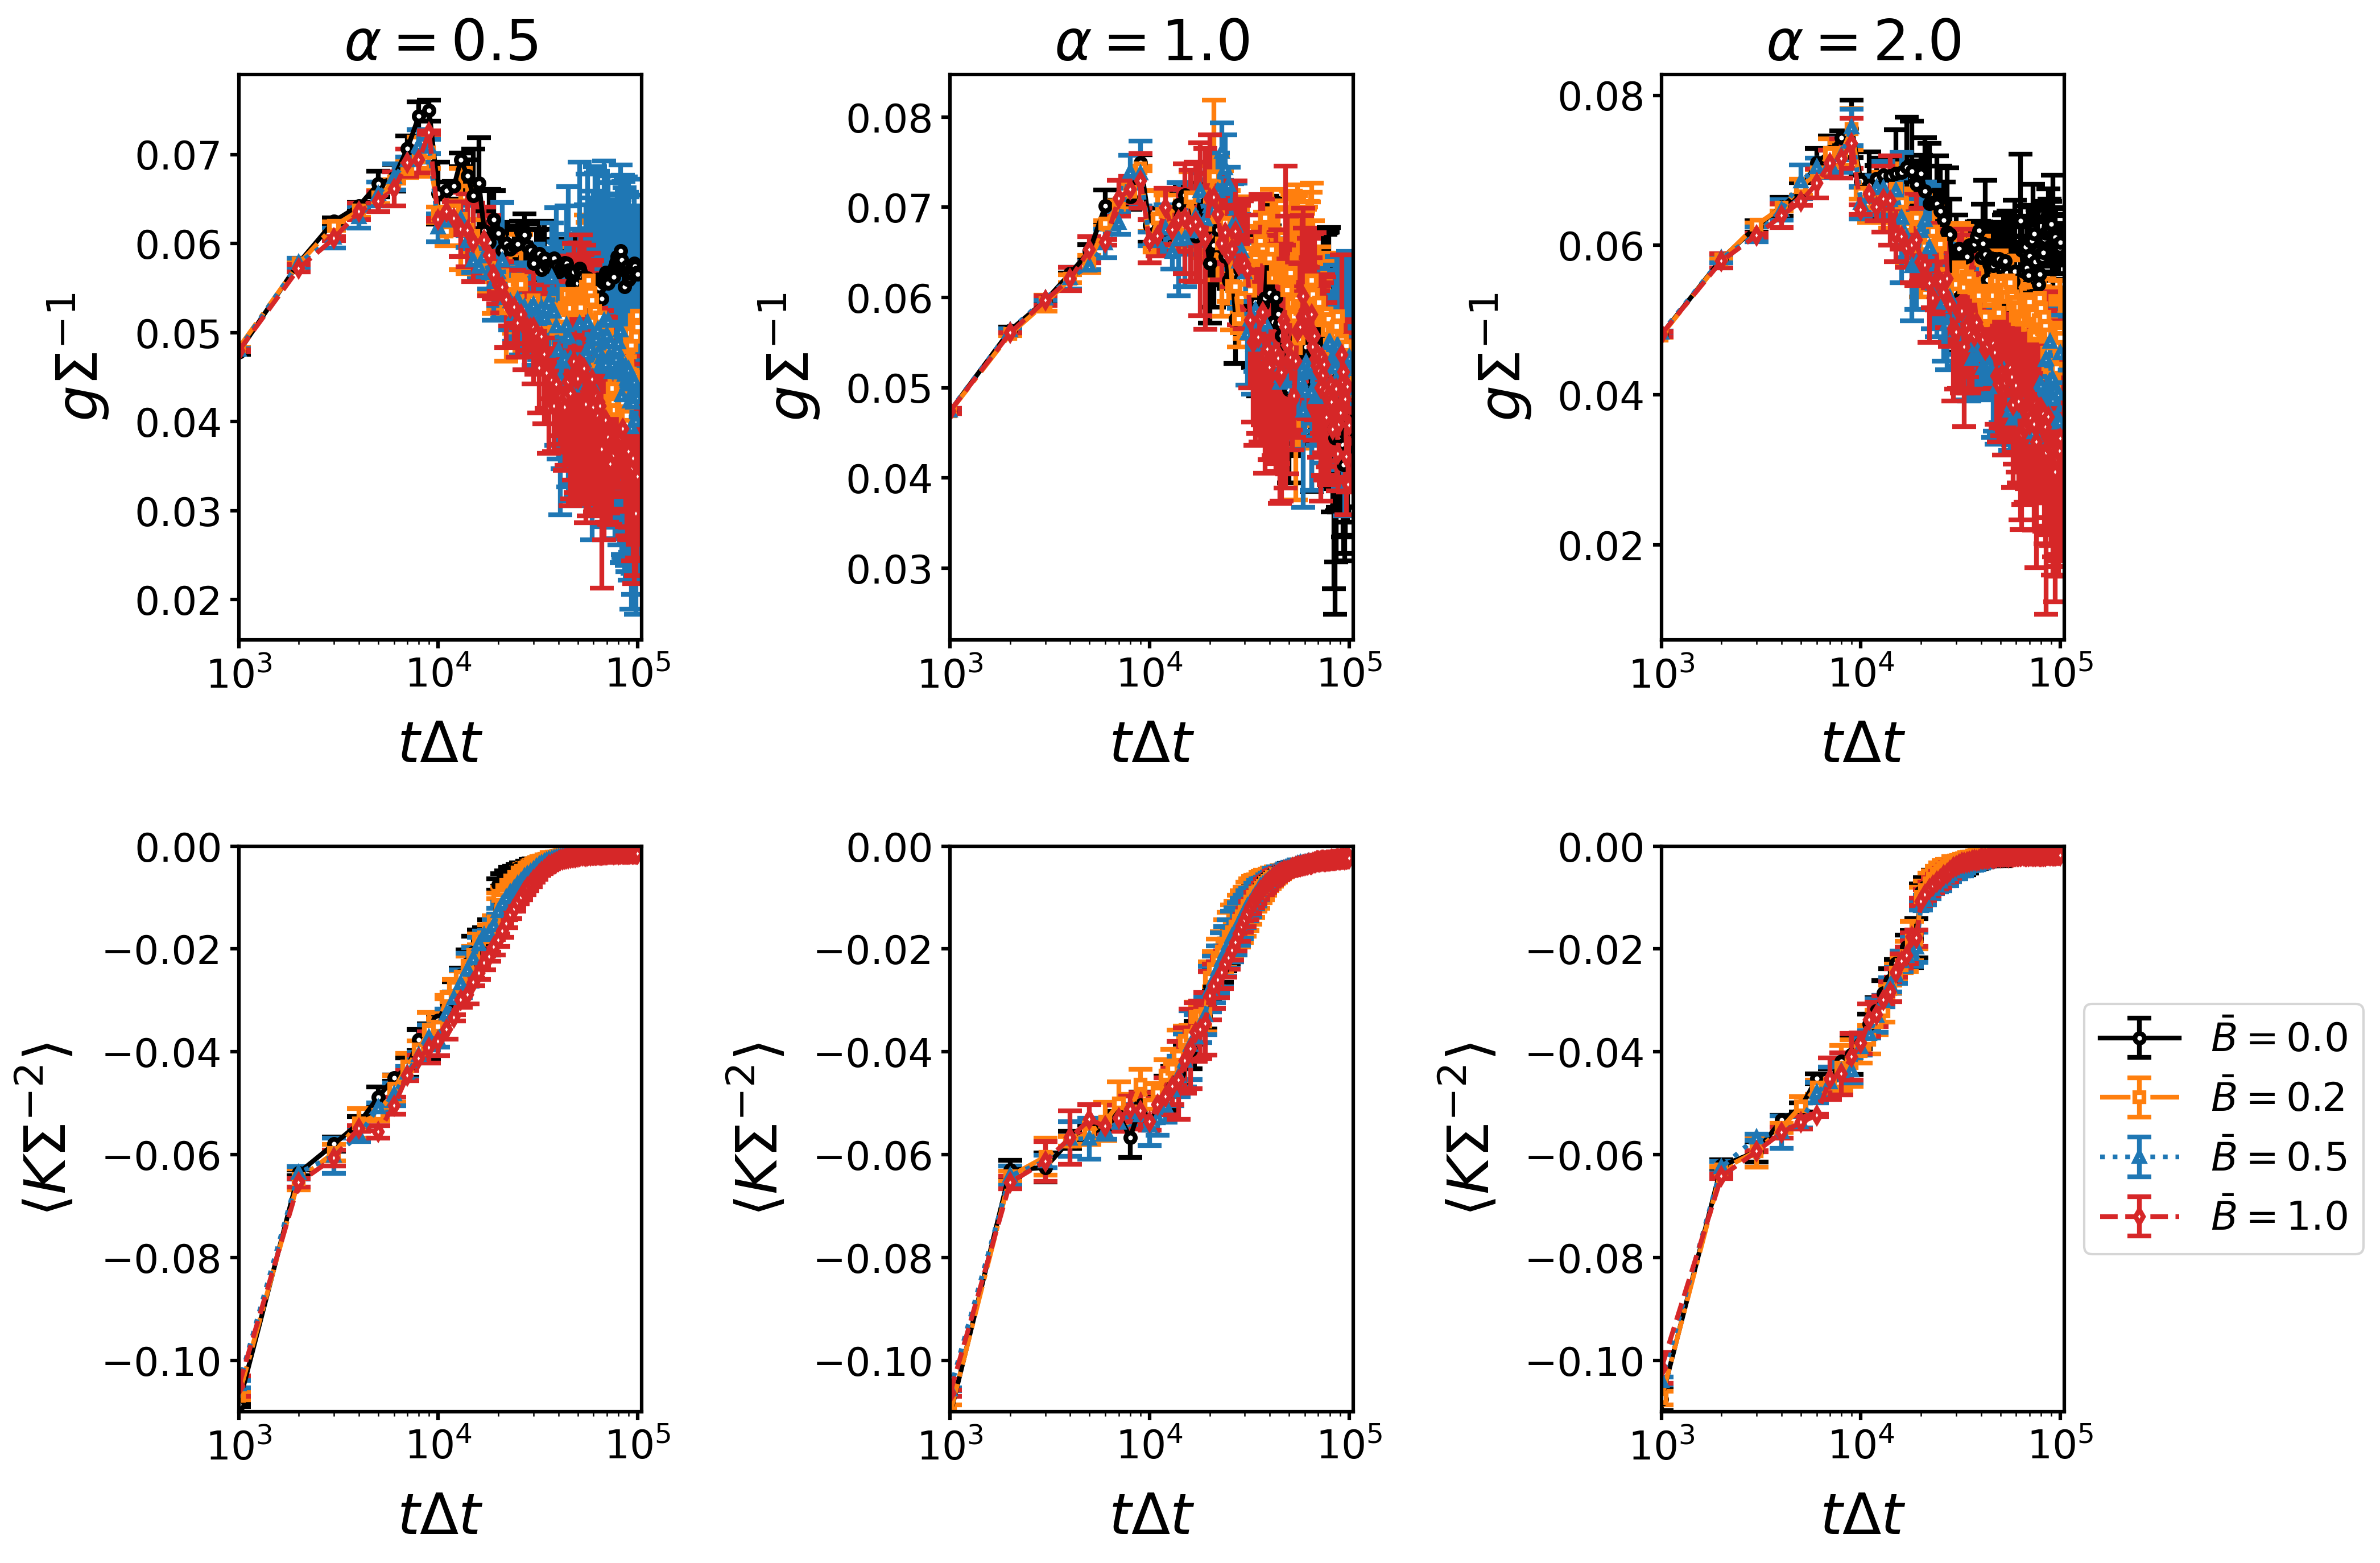
\includegraphics[scale = 0.4]{figures/results/paper1/genus_curvature_vs_coverage.png} 
    \caption{Plots of Gaussian $\langle K \rangle \Sigma^{-2}$ curvature over time averaged across 3 runs. 
    From left to right, I have particles with $\alpha = 0.5, 1, 2$. I observe that the initial stages of 
    evolution are unaffected by the applied magnetic field. However, after about 10000 timsteps, I see a 
    magnetic field dependence on the evolution of the Gaussian curvature. The preservation of this divergence 
    occurs when ellipsoidal particles are used but not spherical particles.} 
    \label{fig:curvature_vs_coverage}
\end{figure}

The time evolution of $g \Sigma^{-1}$ of bijels stabilized with spherical particles is unaffected by the application of a magnetic field. However, a 
slight decrease in the genus as a function of the applied field is observed for bijels stabilized with ellipsoidal particles. This suggests that the 
evolution of the surface corresponding to the interface is changed by the adsorption and orientation of magnetically responsive ellipsoidal particle. 
I see effects of this change in $\langle G \rangle \Sigma^{-2}$ where I see the evolution of the curvature being delayed, indicated as a rightward 
shift of the plots as a function of the applied field. 

Despite all our curvature calculations being normalized with their surface area to volume ratio, I still see curvature differences as a function of the applied 
magnetic field. Experiments have identified that curvature changes can occur due to the formation of monogels, which are particle networks formed from bijels that 
can withstand the remixing of their constituent liquids. \cite{sanz_colloidal_2009, lee_making_2013} This process cannot occur in our simulations as I am utilizing 
electrically neutral particles that only interact through contact forces. Therefore, the change in curvature arises from microstructure changes driven by particle 
alignment to the magnetic field direction. These results provide support for the mechanism of control being due to particle alignment to the magnetic field during 
coarsening changes the topology of the surface, which upon jamming of ellipsoidal particles is locked in. As our particles only interact through contact forces, 
the only mechanism present that can change the topology of the interface would be particle interactions upon contact with each other. Particle interactions are 
controlled through the orientation of particles and the local ordering of particles on the interface. Seeing that there are differences in the gaussian curvature of the bijel,
the domain anisotropy characterized in Figure \ref{fig:D2a_B} may be able to be characterized as changes in the topology of the surface. Chan and Thornton introduced a 
topological technique to characterize the connectivity of surface as a function of a distance from the interface to calculate the channel size distribution. 
\cite{chan_channel_2012} I can use the channel size distribution to investigate how the connectivity of the microstructure and thus the 
channel size is affected as a function of the applied magnetic field.

\begin{figure} 
        \centering 
        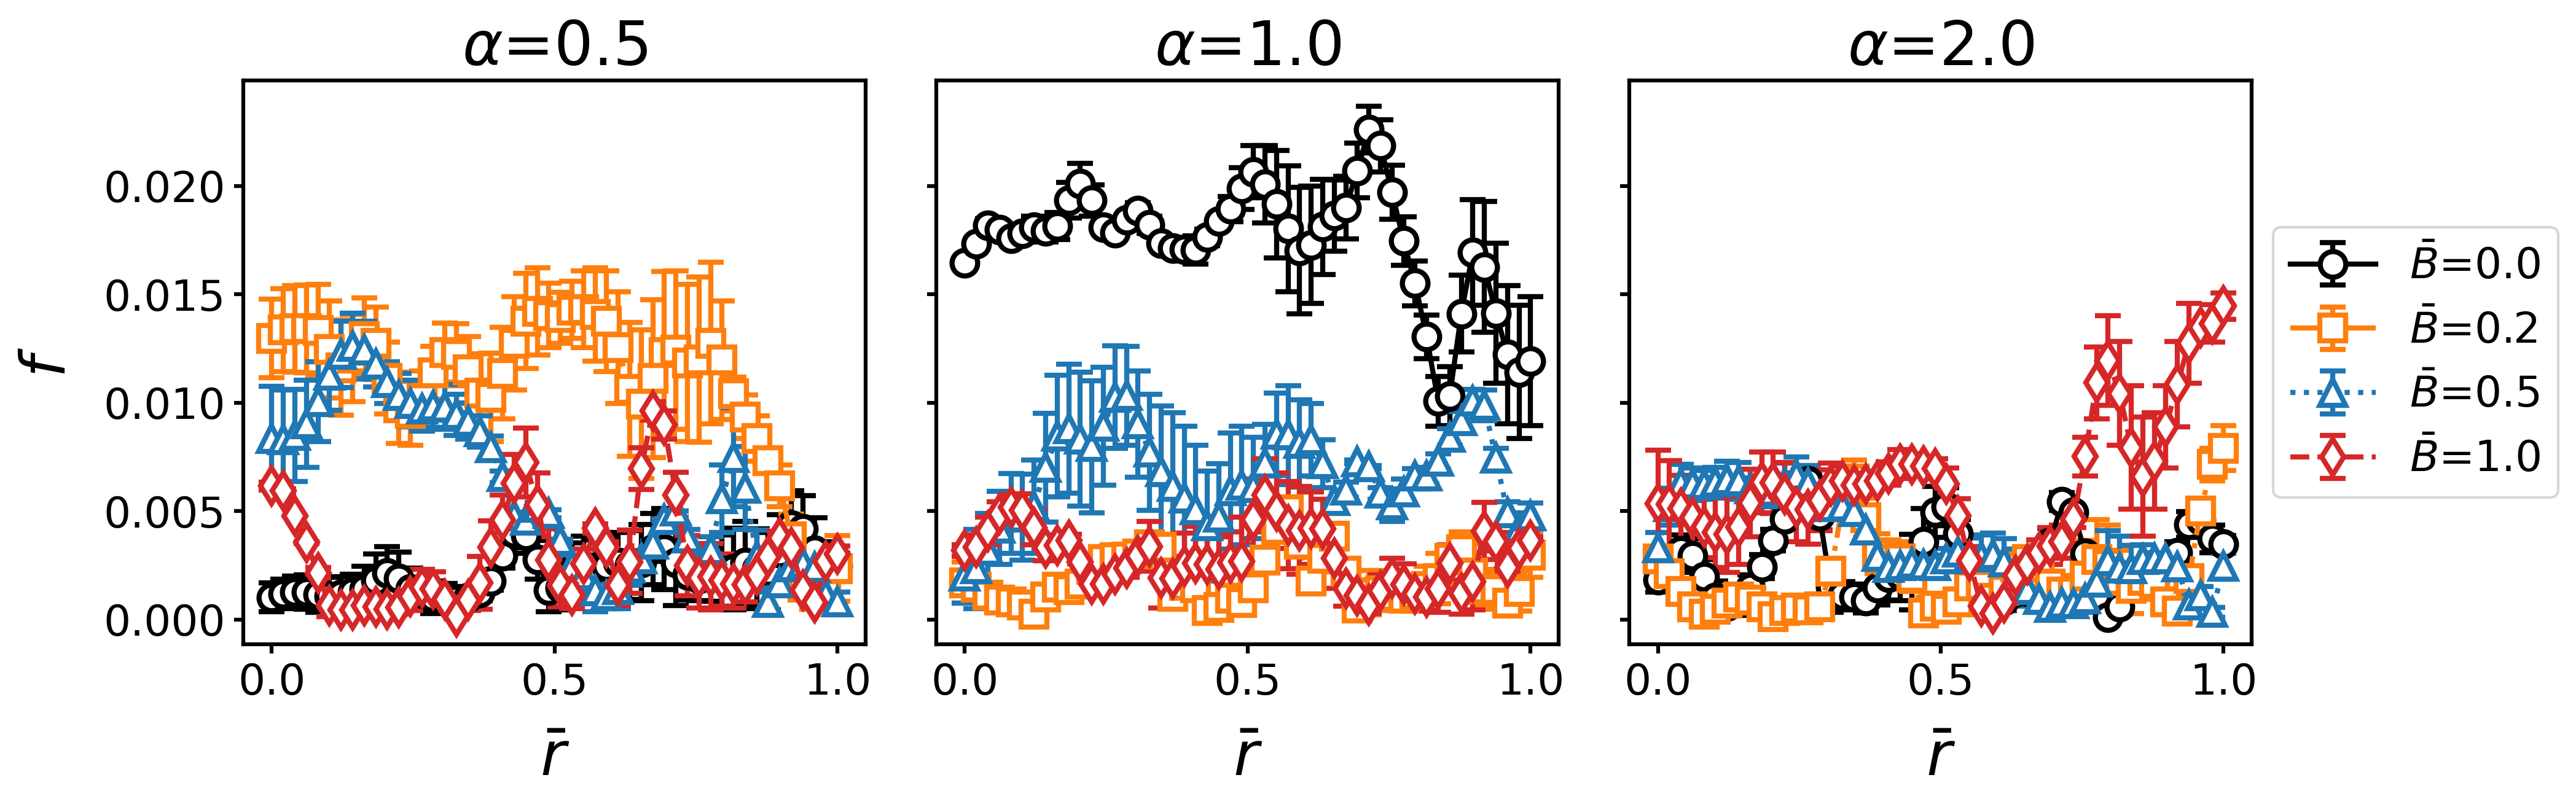
\includegraphics[scale = 0.4]{figures/results/paper1/CSD_ss.png} 
        \caption{Plots of the channel size distribution for bijels stabilized by oblate, spherical and oblate particles at the final timestep plotted
                 against the distance from the interface normalized with the characteristic length scale. The channel sizes obtained are averaged over 
                 three runs. I see that the peak locations are shifted to larger and smaller positions for bijels stabilized with ellipsoidal particles
                 upon field application} 
        \label{fig:CSD_B_ss}
    \end{figure}

While run to run variation is observed, the combined data of the channel size distribution shown in Figure \ref{fig:CSD_B_ss} shows some differences 
in the channel size distribution in each bijel stabilized with ellipsoidal particles. It was expected that the domain anisotropy obtained using second moment of the 
structure factor would manifest as two peaks in the channel size distribution. \cite{karthikeyan_formation_2024} This behavior is observed in the channel size 
distribution for bijels stabilized with ellipsoidal particles with $\bar{B} = 1$, but is more difficult to see when smaller magnetic fields are applied. 
These differences arise from the particle ordering and local distribution changes observed. 

\subsection{Kinetics of bijel formation in magnetic fields}

To shed light on the mechanisms involved in the coarsening dynamics,
I now turn to the kinetics of bijel formation in more detail. The
coarsening dynamics can be characterized by a coarsening speed. Here,
I use the finite difference of the directional domain size to
calculate the components of the coarsening velocity
%
\begin{equation}
u_{L_\beta}(t) = \frac{L_\beta(t+\Delta t_s)-L_\beta(t-\Delta t_s)}{2\Delta t_s} ,
\end{equation}
%
where \(\Delta t_s\) is the time between simulation
snapshots, and $\beta$ denotes either the direction parallel or perpendicular to the magnetic field.

\begin{figure*}
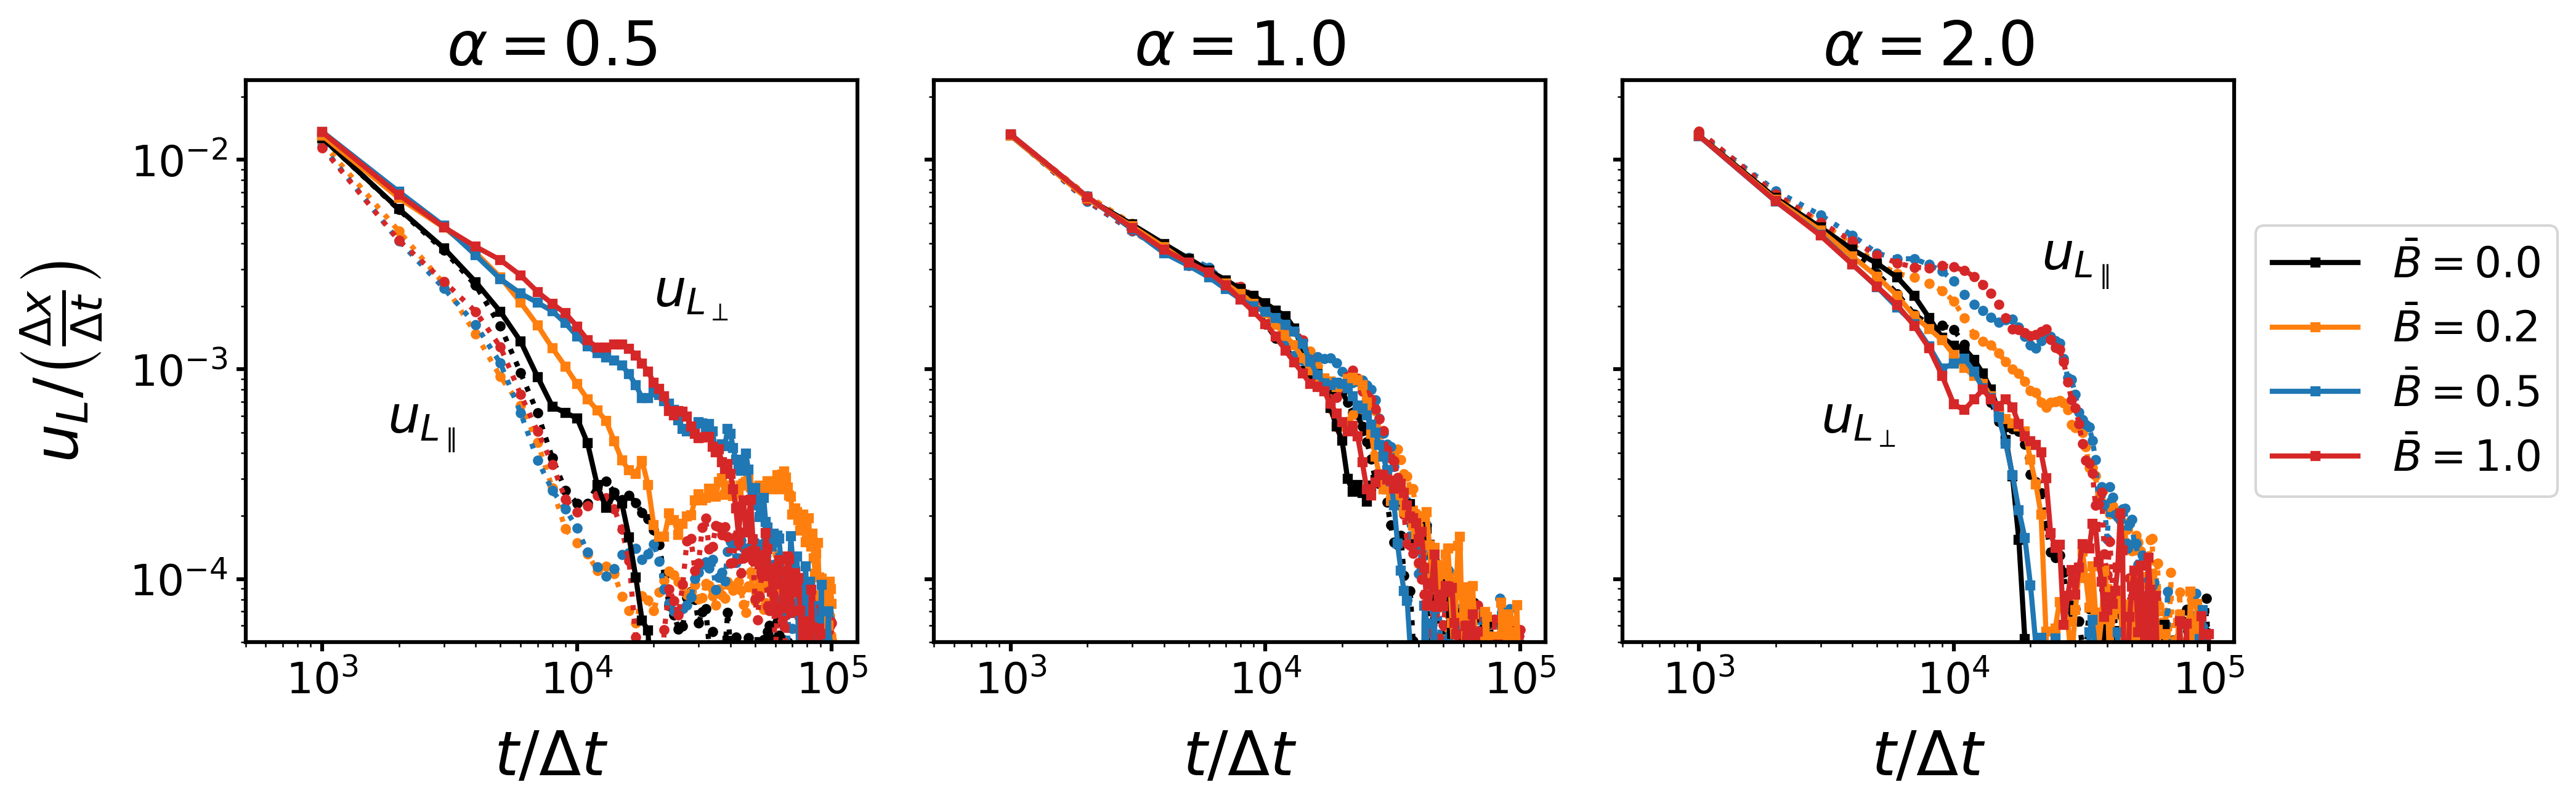
\includegraphics[width=\textwidth]{figures/results/paper1/coarsening_vel.png}
\caption{Time-dependence of the coarsening velocity $u_L$ for different particles shapes $\alpha$  
and at different magnetic field strength $\bar{B}$. The different components of the coarsening velocity 
show that the jamming time is different in the direction parallel and perpendicular to the magnetic field.}
\label{fig:coarsening_velocity}
\end{figure*}

Figure \ref{fig:coarsening_velocity} shows the coarsening speed in the directions parallel and perpendicular to the applied magnetic field. 
The data confirms that for spherical particles, domain coarsening remains isotropic. I observe a higher coarsening speed initially which slows 
at later times when the particles begin to jam. This indicates that the
coarsening is subject to different time scales, as reported previously
by Harting and co-workers \cite{gunther_timescales_2014}. Reeves et
al.~\cite{reeves_particle-size_2015} have pointed out that bijel
formation hinges on the jamming time in relation to the disruption time, i.e., the time scale at which domain pinch-off events can cause bijel break-up through 
depercolation. In our simulations, however, I have not observed disruption of bijel formation; stable bijels form for all parameters consistent with simulations 
by Stratford et
al.~\cite{stratford_colloidal_2005} and Jansen et al.~\cite{jansen_bijels_2011}.

For ellipsoidal particles, our data clearly shows that an\-isotropic
domain coarsening arises in magnetic fields.  For oblate particles
(\(\alpha=0.5\)), the coarsening speed in the direction perpendicular
to the field increases with increasing magnetic field strength.
Jamming in this direction appears to be delayed compared with the
direction parallel to the field. The coarsening speed in the parallel
direction remains comparable to the case without an applied magnetic
field. This anisotropic behavior of the coarsening speed reverses for
prolate particles, where the coarsening speed in the direction parallel to the field increases with increasing field strength, and jamming in this direction
is delayed compared with the perpendicular direction. In addition, I observe a shoulder (around \(10^4\Delta t\)) where the coarsening speed decays more slowly before jamming sets in. These results suggest that the coarsening near the jamming time is affected by a mechanism that depends on the applied magnetic field and causes the anisotropic
behavior. This mechanisms involves the re-orientation of anisotropic
particles and their alignment relative to the direction of the
magnetic field. To confirm this hypothesis, I analyze the
orientational order of the particles and their alignment relative to
the magnetic field and the interface, respectively.

\subsection{Particle re-orientation and packing}

\begin{figure}
\centering
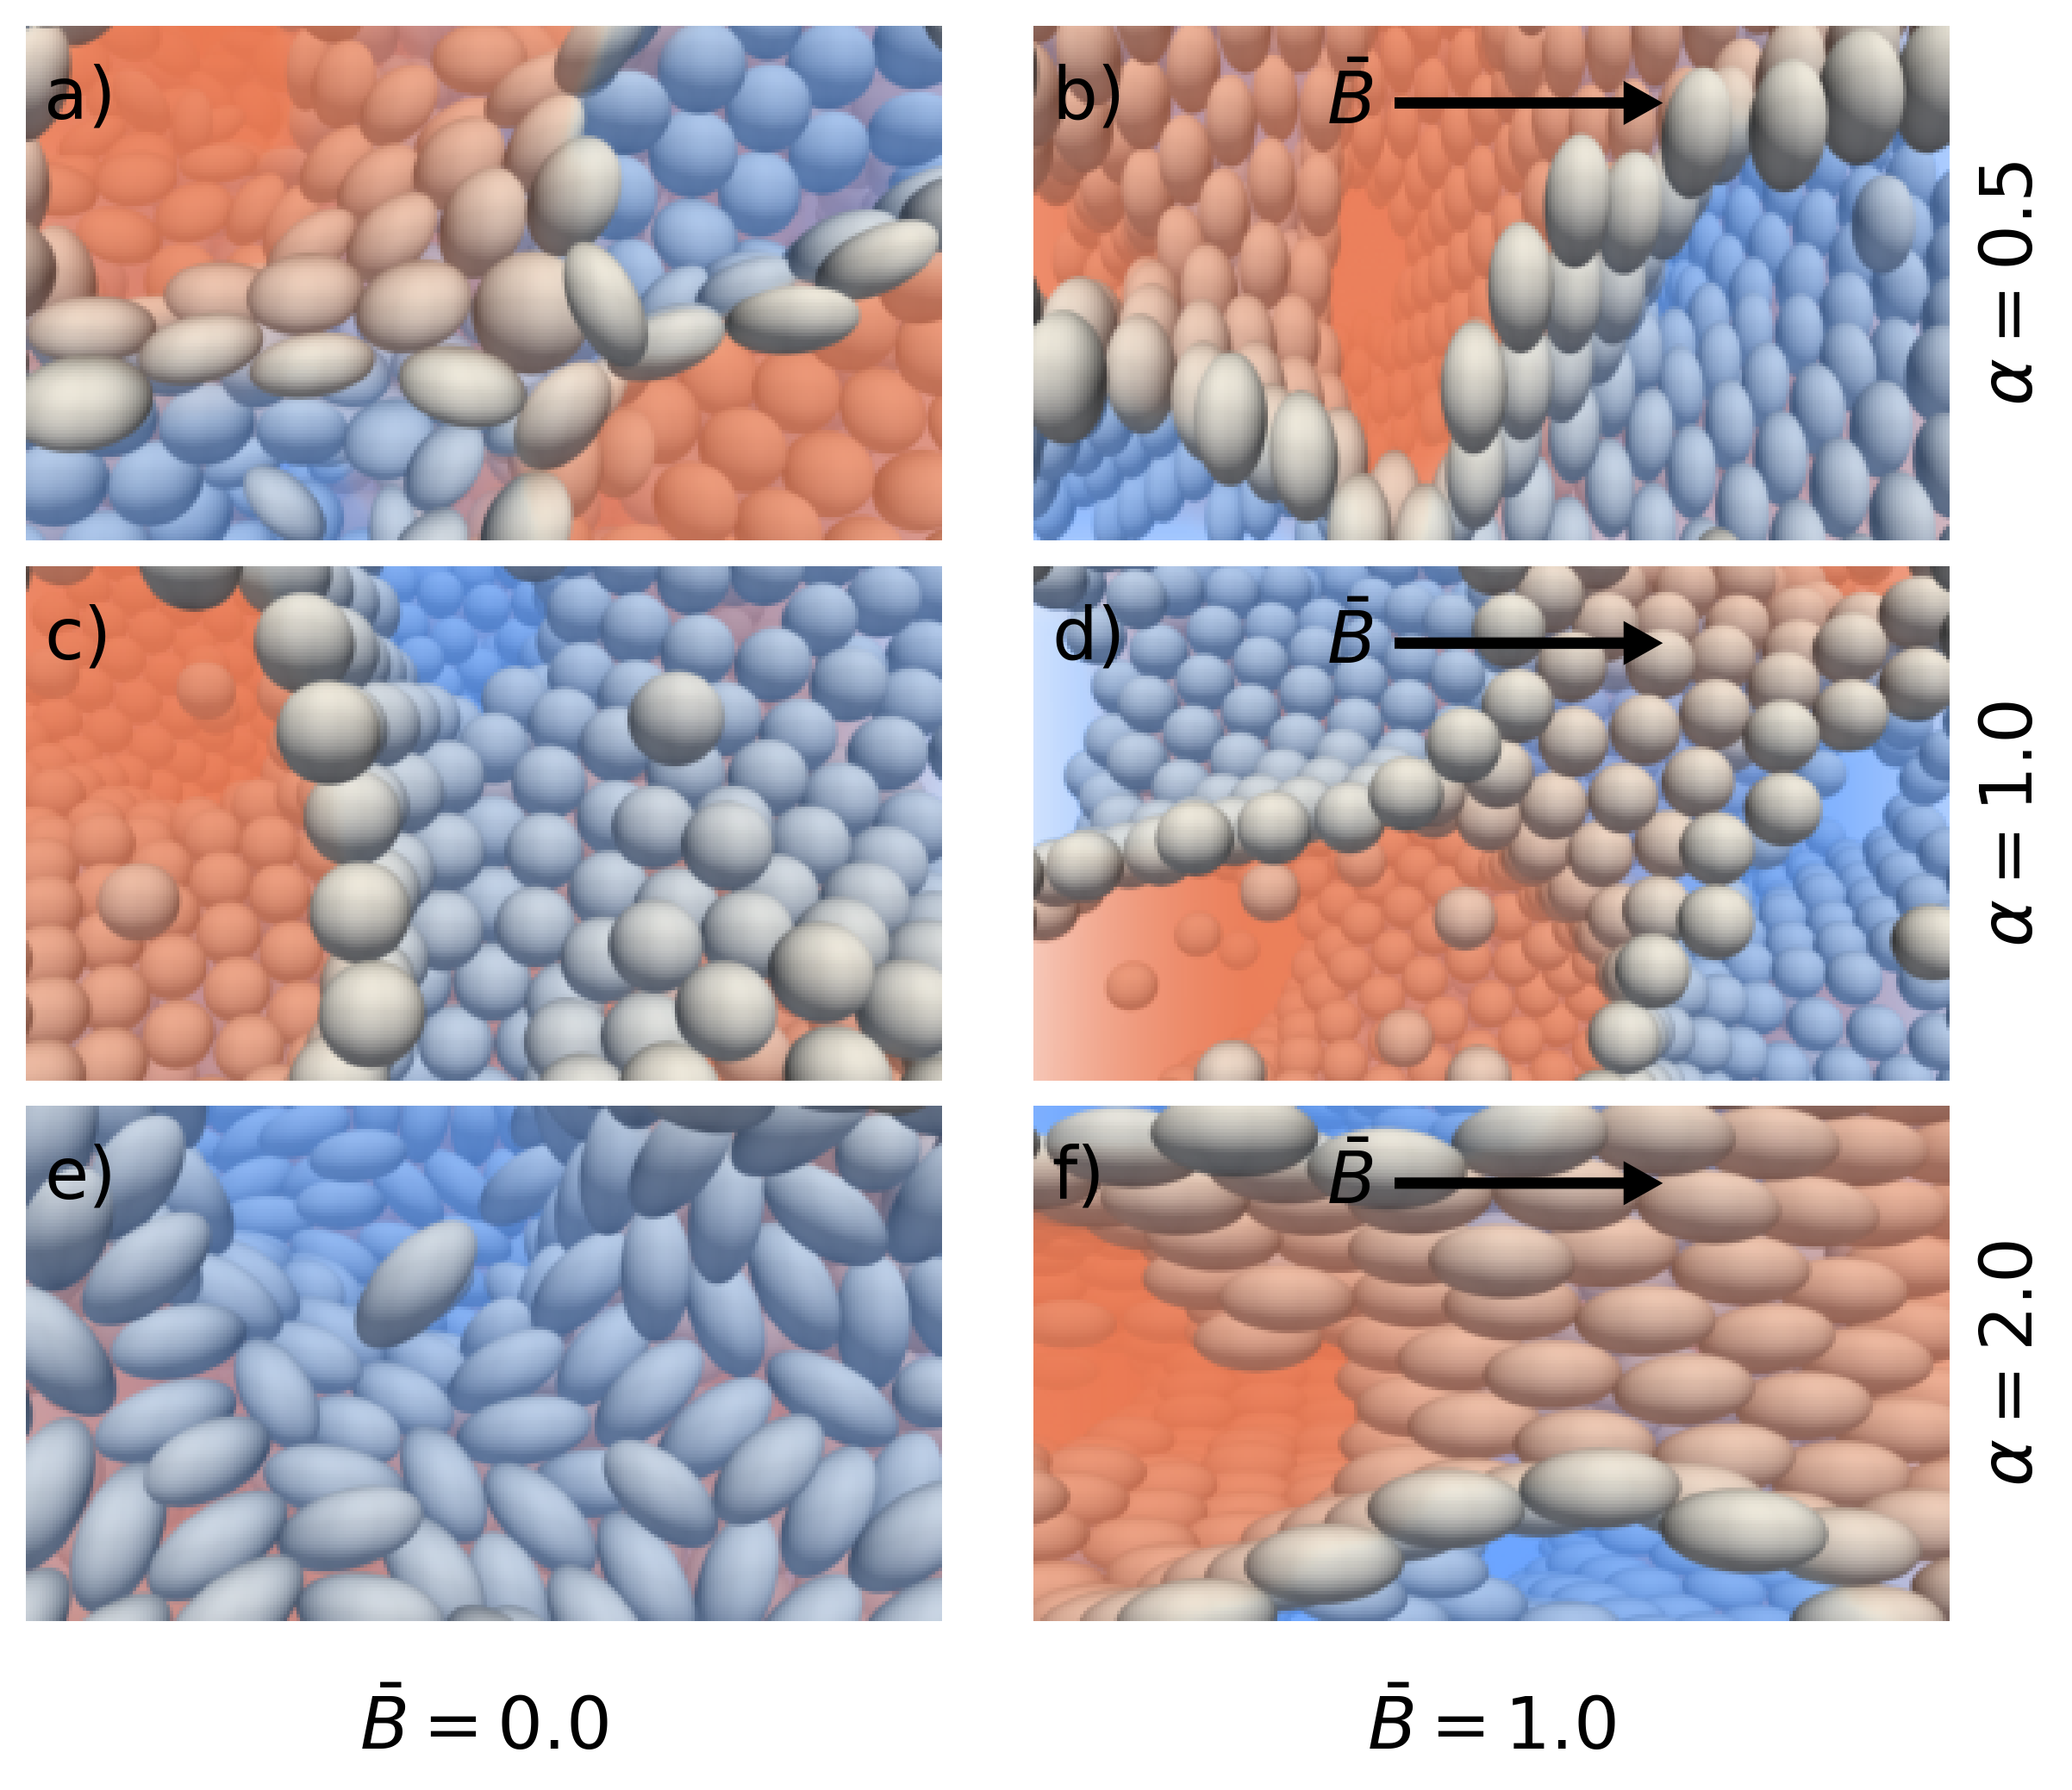
\includegraphics[width=0.5\columnwidth]{figures/results/paper1/particle_packing_viz.png}
\caption{Snapshots illustrating the particle packing at the interface for different particle shapes $\alpha$ with (left) 
        and without (right) applied magnetic field $\bar{B}$. The right column shows the alignment of the symmetry axis of 
        the oblate (top row) and prolate (bottom row) particles in the direction of the magnetic field indicated by arrows.}
\label{fig:packing_viz}
\end{figure}

The primary effect of the magnetic field is the torque it exerts on the
magnetic dipole of the particles. This torque rotates the particles
towards the direction of the magnetic field. The alignment of the
particles with the field direction can be clearly observed in the
simulation snapshots shown in Figure \ref{fig:packing_viz}. While the
particles are oriented randomly in the interface in the absence of a
magnetic field (\(\bar{B}=0\)), the magnetic field induces orientational
order of the magnetic dipoles (shown for \(\bar{B}=1\)).

\begin{figure}
\centering
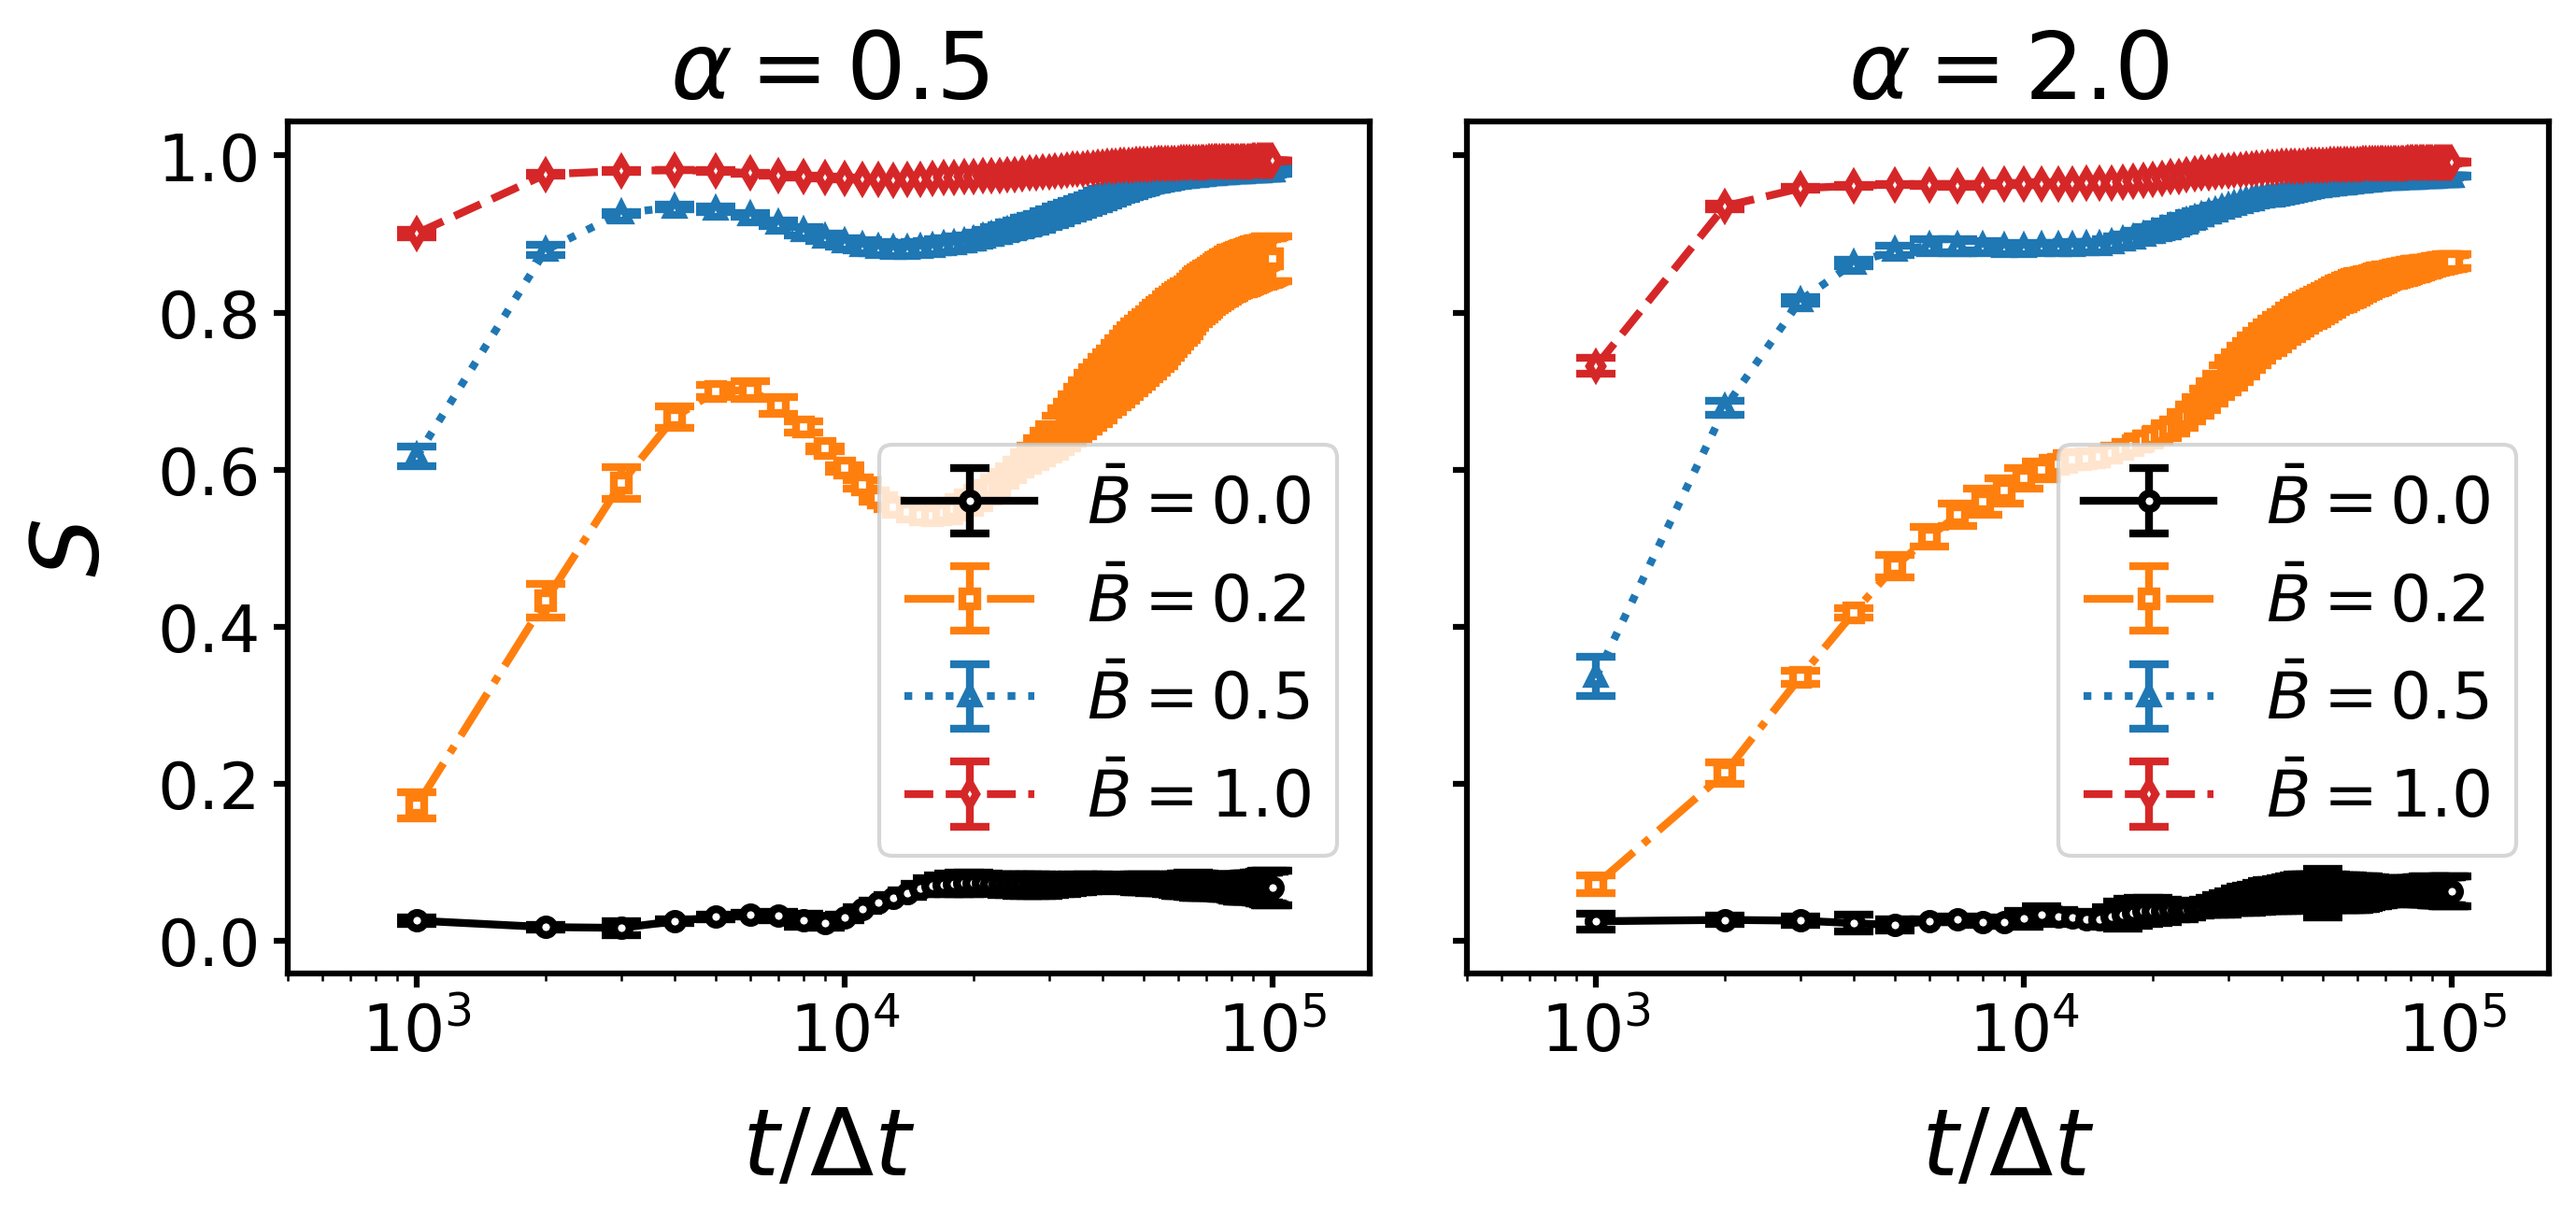
\includegraphics[scale = 0.4]{figures/results/paper1/S-vs-t.png}
\caption{Time-dependence of the nematic order parameter $S$ of oblate ($\alpha=0.5$) and prolate ($\alpha=2$) 
        particles at different field strength $\bar{B}$. Errorbars indicate the standard deviation taken over 
        three independent simulation runs. Nematic order generally increases with applied field strength for all particle geometries. 
        The increase slows down (for prolate particles) or reverses (for oblate particles) around $10^4$ timesteps.}
\label{fig:nematic_time}
\end{figure}

To measure the particle alignment quantitatively, I computed the
nematic order tensor using the method detailed in Section \ref{section:nematic_order_parameter} 
Figure \ref{fig:nematic_time} shows the time evolution of the nematic
order parameter \(S\) for the three different particle aspect ratios
\(\alpha\) and varying magnetic field strength \(\bar{B}\). The onset of
orientational order is nearly instantaneous and increases with
increasing field strength. For magnetic flux densities
\(\bar{B}\ge0.5\), the nematic order parameter saturates at
\(S\approx 1.0\) towards the end of the simulation. For the prolate
particles (\(\alpha=2.0\)), I observe a shoulder at around
\(10^4\Delta t\) and an intermittent plateau. The occurrence of this
plateau coincides with the slowed decay of the coarsening speed in Fig.
\ref{fig:coarsening_velocity}. This change in the orientational ordering
is even more distinct for the oblate particles, where the nematic order
decays intermittently before it increases again. The intermittent decay
for oblate particles, and the plateau for prolate particles, correlate
with the delayed onset of jamming in the direction perpendicular and
parallel to the magnetic field, respectively. These observations can be
interpreted as follows: The magnetic field aligns the particles with the
direction of the magnetic field early during the simulation. Due to this
alignment, the steric constraints between particles adsorbed at the
interface are reduced which allows further coarsening of the interfacial
area. However, during coarsening, the interfaces may re-orient
themselves and cause a capillary torque on the particles that competes
with the magnetic torque. This competition intermittently perturbs the
nematic order of the particles leading to the observed decay and plateau
of the nematic order parameter. Accordingly, the decay of \(S\) is most
pronounced at the weakest magnetic field \(\bar{B}=0.2\). To further corroborate 
this mechanism, I plot the time evolution of the orientational order of the interfaces. 

\begin{figure}
\centering
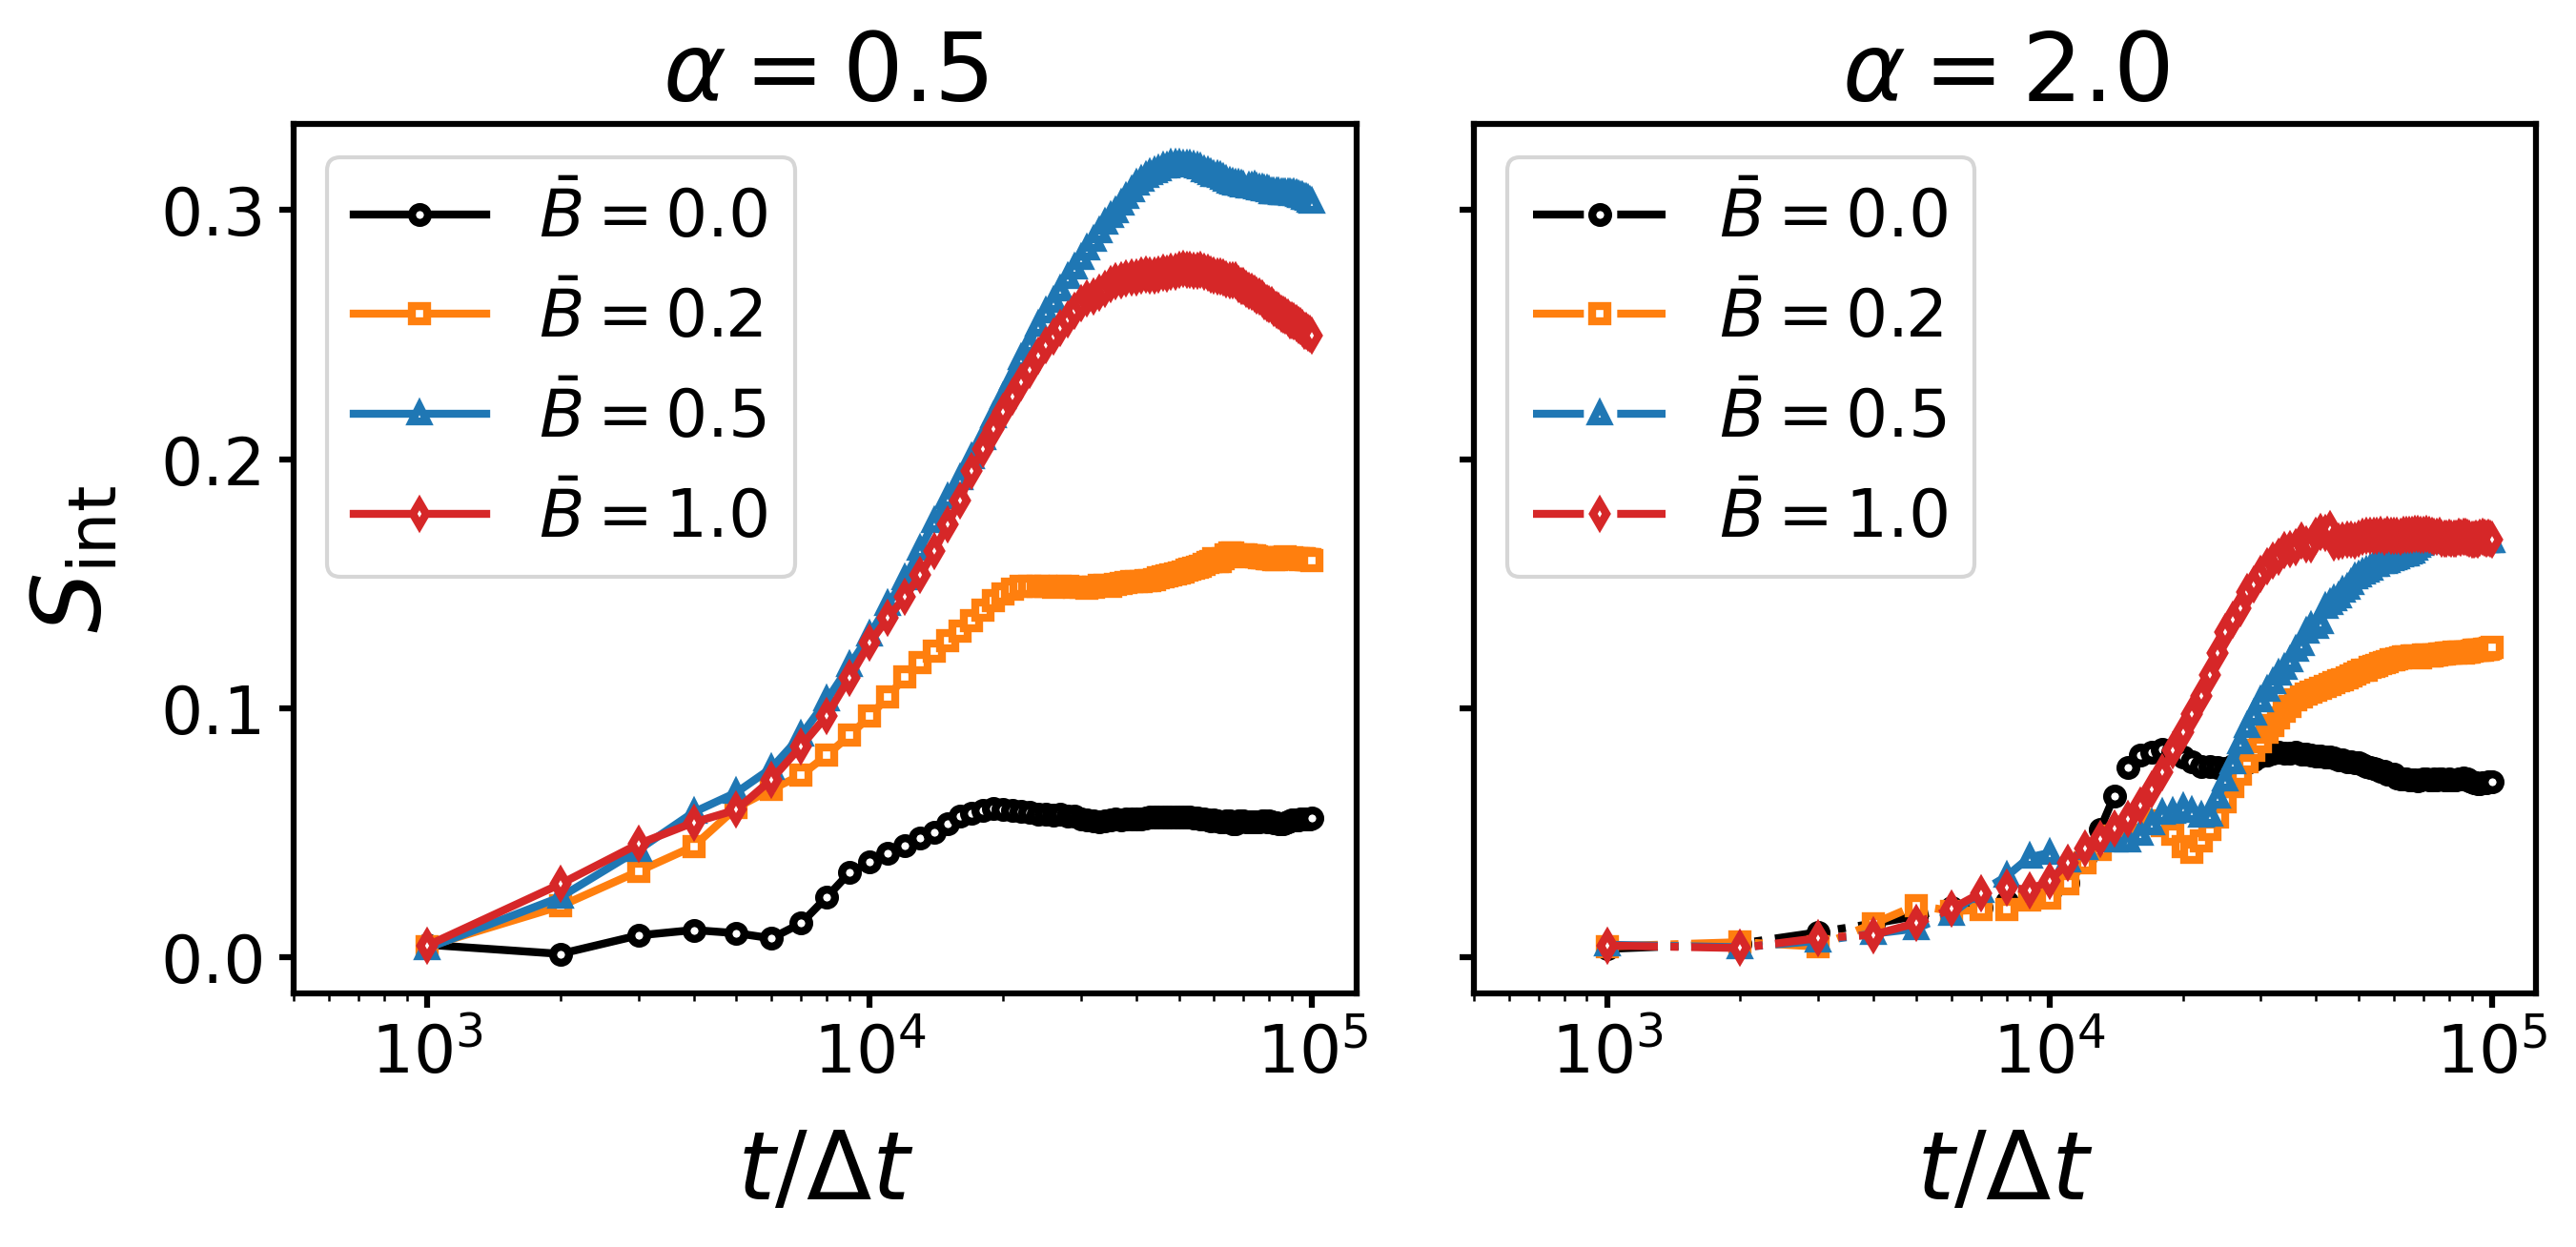
\includegraphics[scale = 0.4]{figures/results/paper1/interface_nematic.png}
\caption{Time-dependence of the interface nematic order for oblate ($\alpha=0.5$) and prolate ($\alpha=2$) particles at different magnetic field strength $\bar{B}$. The interface alignment tends to increase with increasing field strength. The rate of increase becomes larger around $10^4$ timesteps, indicating the alignment of the interfaces due to capillary interactions with the particles.}
\label{fig:interface_nematic}
\end{figure}

The results for the interface nematic order parameter $S_{\text{int}}$
are shown in Figure \ref{fig:interface_nematic}. The nematic interface
alignment increases over time and the rate of increase appears to be
higher for larger magnetic field strength $\bar{B}$. In all cases, the
final value of $S_{\text{int}}$ is below 0.5 indicating that the
tortuous structure of the interface is maintained in the presence of
magnetic fields. This confirms that the re-orientation of the particles
does not disrupt the bijel structure but leads to partial alignment of
the interfaces without changing the general topology of the bicontinuous
morphology.

When the particles rotate, the interface exerts a capillary torque on
the particles due to the surface tension and the contact angle. If the
magnetic torque exceeds the interfacial forces, the particles can
potentially overcome the capillary torque and rotate out of the
interface. For prolate particles (\(\alpha=2\)) adsorbed at flat
interfaces, Davies et al. have shown that a transition between the
energetically preferred ``flat'' orientation and a tilted orientation
occurs at a critical field strength of approximately \(\bar{B}=0.2\)
\cite{bresme_orientational_2007,davies_interface_2014,newton_influence_2014}.
In the case of bijels, however, the percolating interfaces are tortuous
and thus more mobile. I therefore posit that, rather than tilting out
of the interface, rotating particles can ``pull'' the interface along
and thereby align the liquid domains. For anisotropic particles, we
expect that the interfaces align along the larger cross-section of the
particles, i.e., perpendicular to the symmetry axis of oblate particles
and parallel to the symmetry axis of prolate particles. The data for the
anisotropic domain size and tortuosity above is consistent with this
assumption. To ascertain that the particles remain indeed in their
energetically preferred orientation with respect to the interface, we
analyzed the angle between the symmetry axis of the particles and the
interface normal calculated using the technique defined in Section 
\ref{section:interface_angle}. Figure \ref{fig:psi_time} shows the time-dependence of the average angle
\(\psi\) between the particle dipole axis and the nearest interface normal.

\begin{figure}
\centering
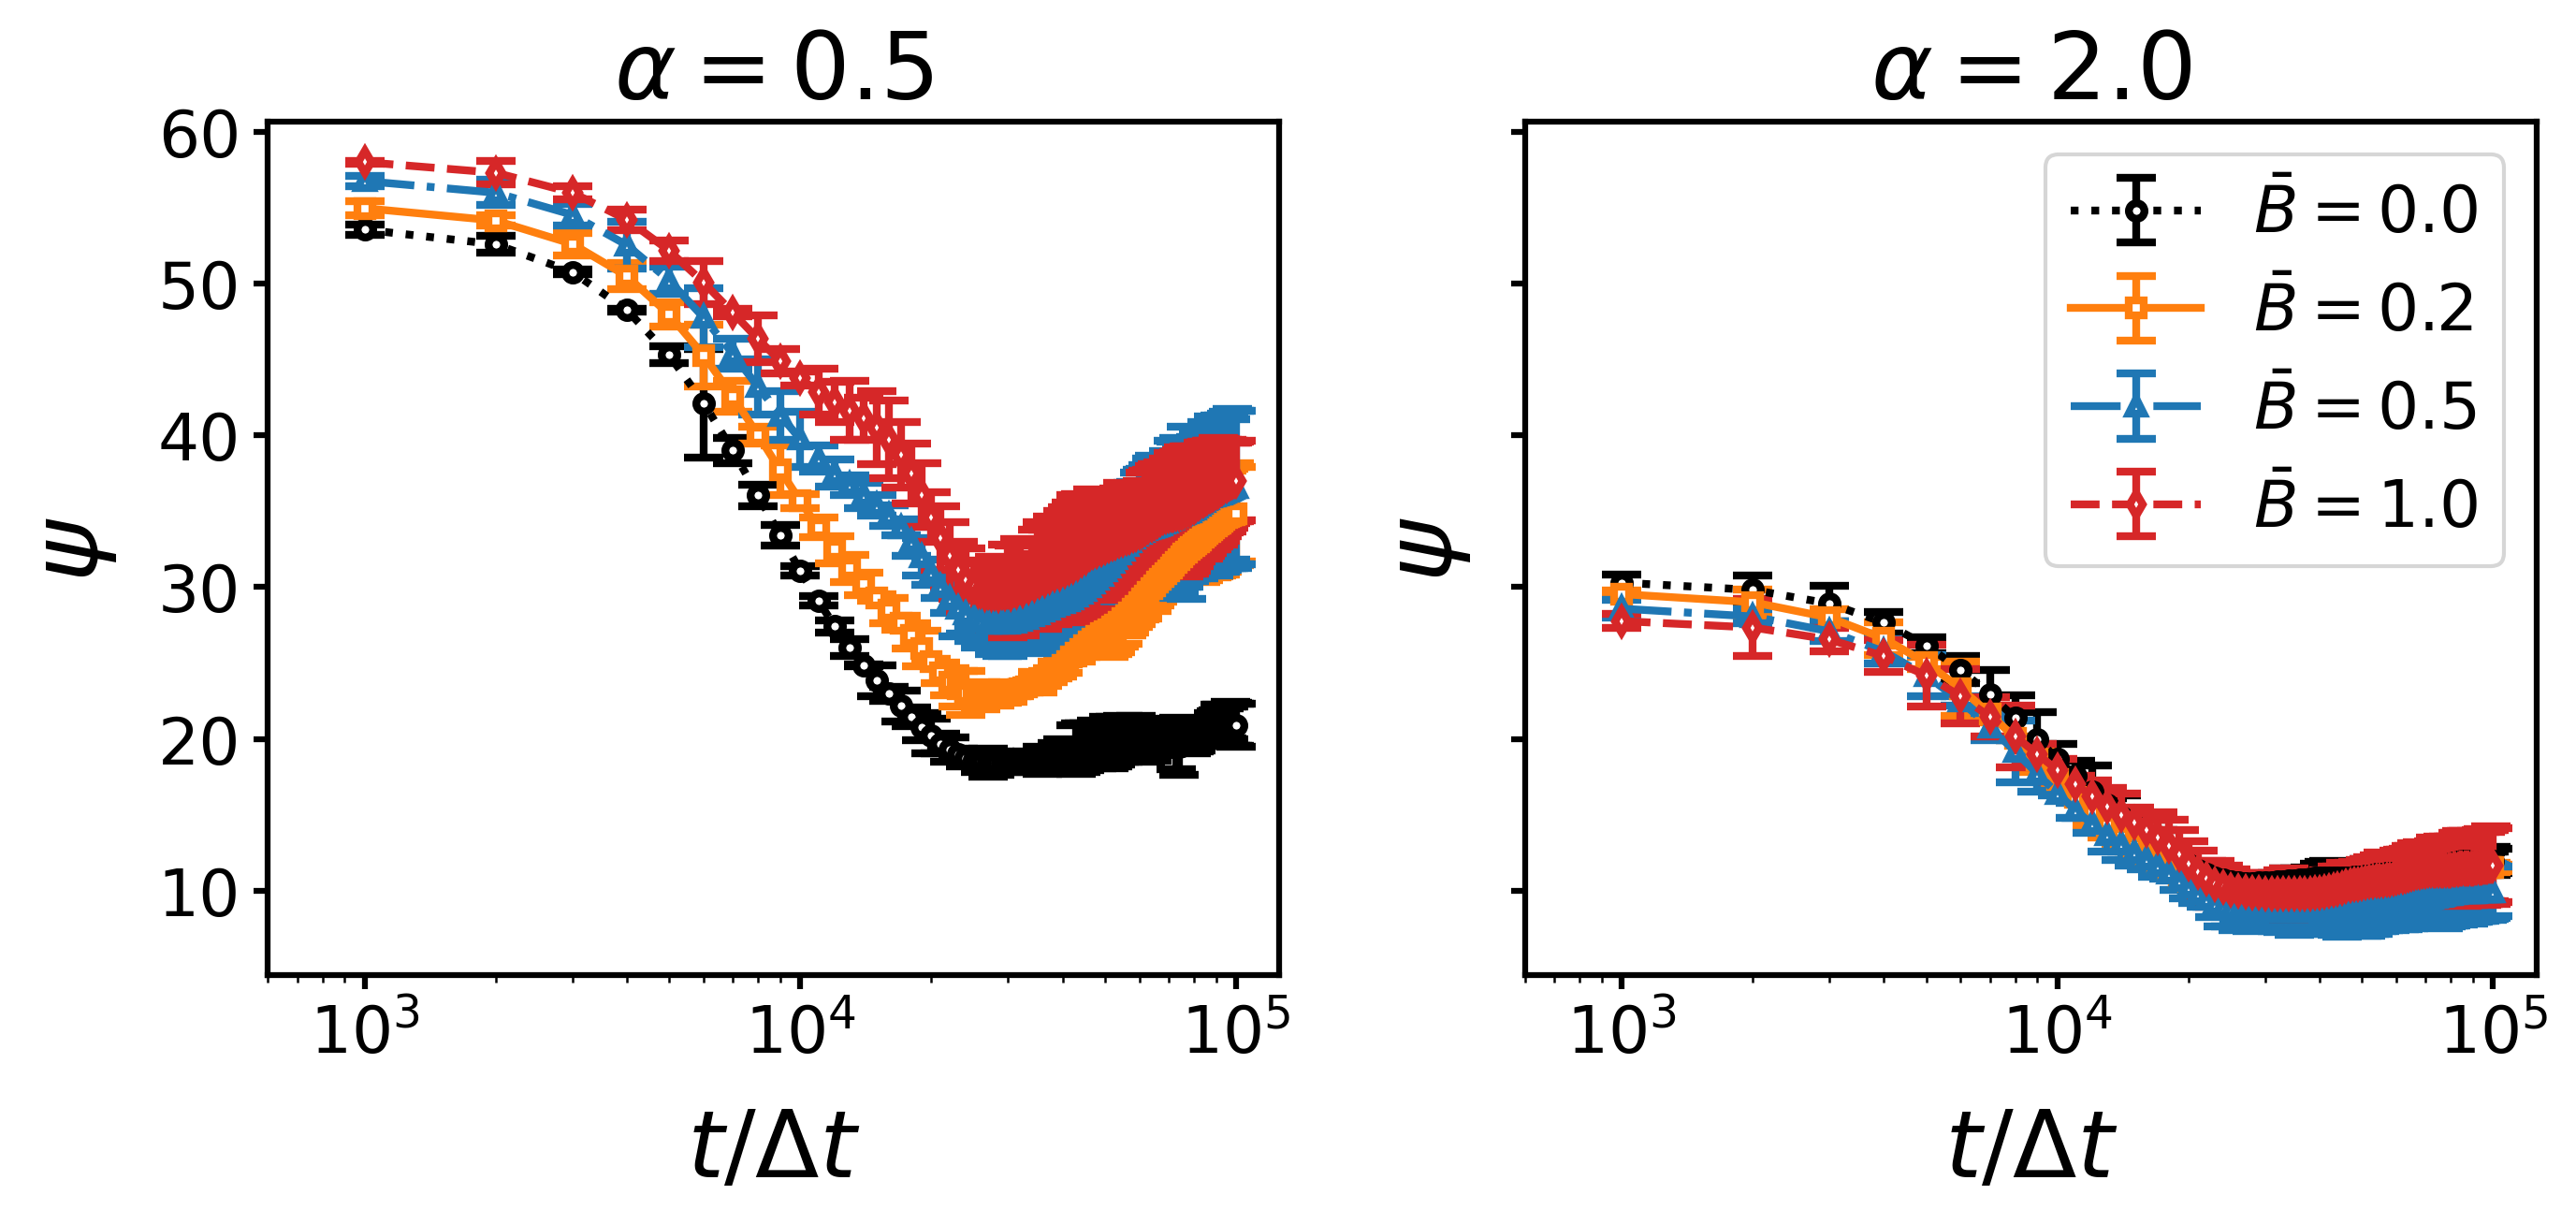
\includegraphics[scale = 0.4]{figures/results/paper1/psi-vs-t.png}
\caption{Time-dependence of the average angle $\psi$ between the particle axis and the 
        interface normal for oblate ($\alpha=0.5$) and prolate ($\alpha=2$) particles at different 
        magnetic field strength $\bar{B}$. Errorbars indicate the standard deviation taken over three 
        independent simulation runs. The angle between between the particles and the interface normal generally 
        approaches the energetically preferred value ($0^\circ$ for oblate particls, $90^\circ$ for prolate particles).
        The average angle changes most rapidly around $10^4$ timesteps.}
\label{fig:psi_time}
\end{figure}

For both types of anisotropic particles, the average angle between the
particle dipole and the interface normal is initially around
\(\psi\approx60^\circ\). As the spinodal interface sweeps through the
system, particles attach to the interface and alignment due to the
capillary torque sets in. For oblate particles, the dipole axis aligns
with the interface normal as indicated by the decay of \(\psi\) towards
zero. For prolate particles, the preferential alignment of the dipole
axis is parallel to the interface and hence \(\psi\) increases towards
\(90^\circ\). The main variation of \(\psi\) occur in a time interval
around \(10^4\Delta t\) which coincides with the distinct features of
the coarsening speed and the particle nematic order observed above. The
results thus substantiate the proposed mechanism of particle
re-orientation in the magnetic field and the concomitant local alignment
of the interface. Once the particles start jamming, the shrinking
interfacial area forces some particles out of their preferred alignment
with the interface, leading to an increase of \(\psi\) for oblate
particles and a decrease of \(\psi\) for prolate particles. Figure
\ref{fig:psi_time} suggests that the forced tilting is more pronounced
for oblate particles than for prolate particles. Due to the larger
aspect ratio, the tilting of prolate particles relative to the interface
induces deformations that appear to cause a larger capillary torque than
the tilting of oblate particles. %For oblate particles, the liquid-solid
%contact line is on average further away from the particle center than
%for prolate particles, hence the lever effect of oblate particles is
%weaker and allows larger tilting relative to the the preferred alignment
%with the interface.
Hence the prolate particles remain mostly aligned with the interface
even in the stronger applied magnetic fields. I plot the interface angle of bijels
stabilized by ellipsoidal particles at the final timestep to demonstrate the differences
that the application of magnetic fields have on the particle monolayer.

\begin{figure}
        \centering
        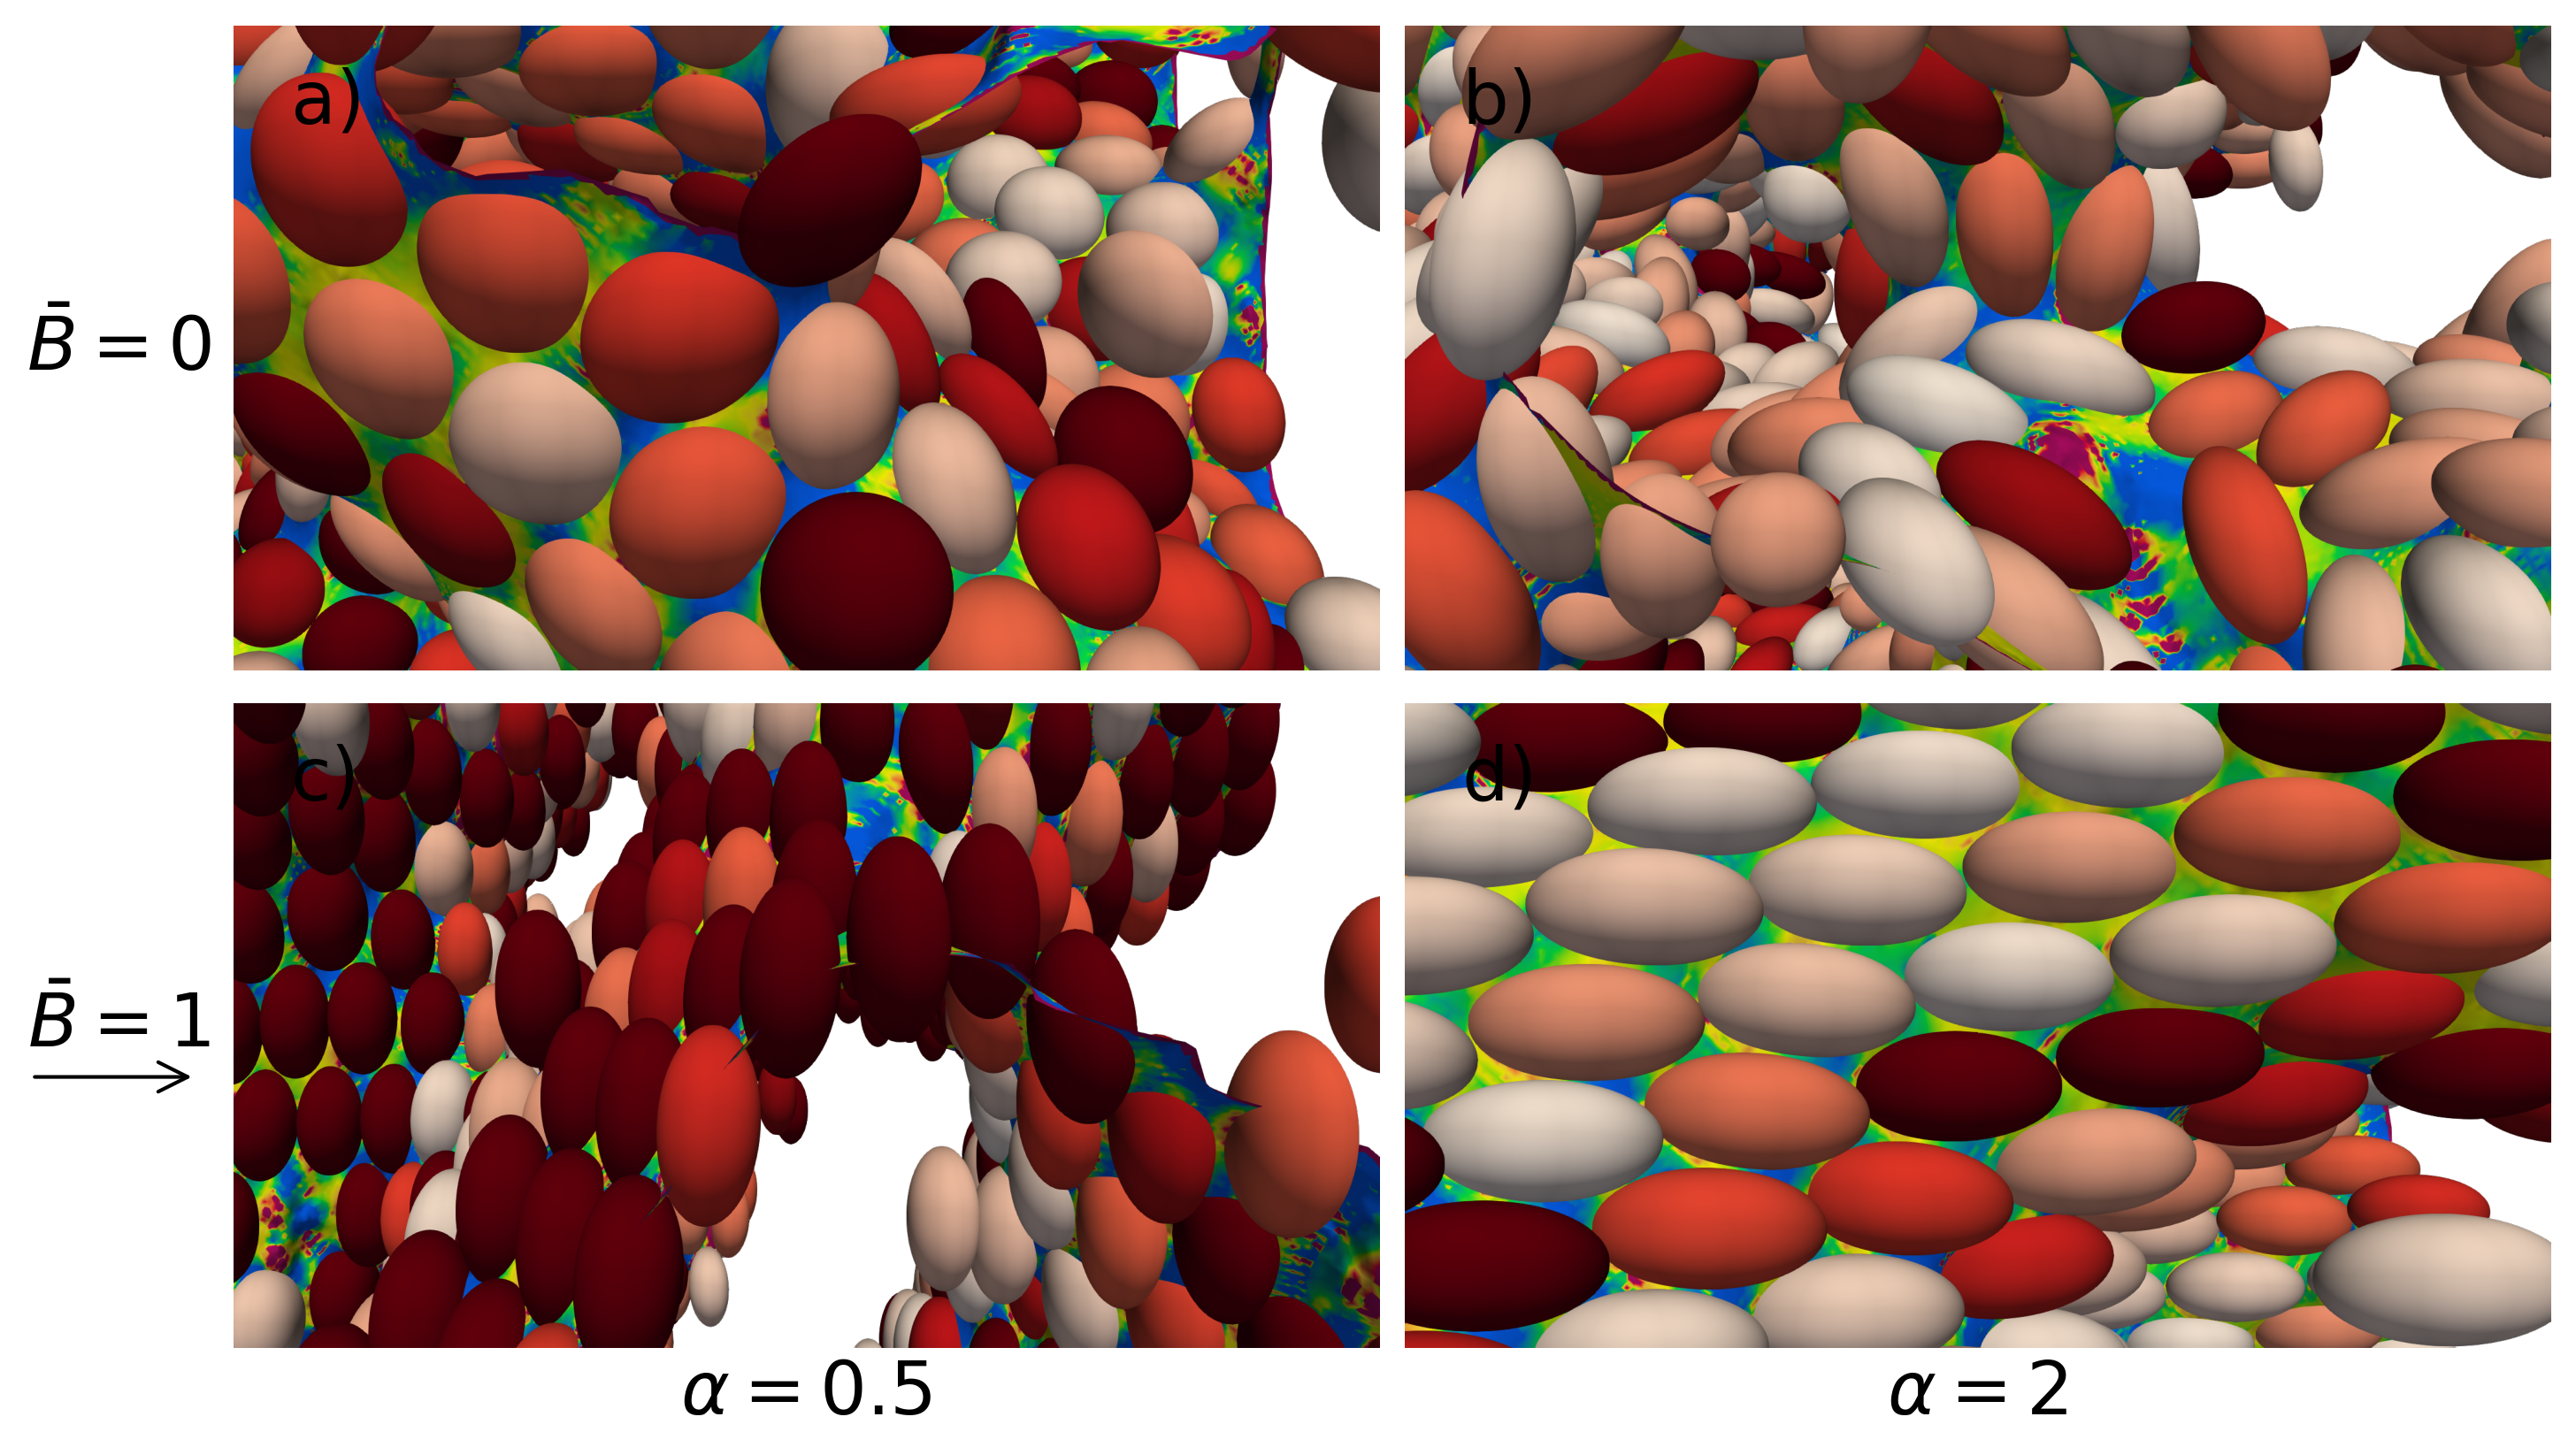
\includegraphics[scale = 0.4]{figures/results/paper1/psi_concat.png}
        \caption{Visualizations of the particle monolayer at the last timestep shaded with the interface angle of each particle in red. The top and bottom
                 rows correspond to snapshots of bijels with no field and a field strength of $\bar{B} = 1$ applied. I see that the oblate particles flip
                 out of the interface into a non energetically favored position while the bijels stabilized with prolate particles tilt out of the interface
                 but are less likely to flip out.}
        \label{fig:psi_viz_ss}
\end{figure}

From Figure \ref{fig:psi_viz_ss} I can see the differences in the particle alignment to the interface characerizing the differences in $\psi$ observed. Oblate
particles can be seen to tilt out of the interface more readily than prolate particles at the same magnetic field strength. Due to the strong surface tension
between the fluids, the particles are strongly adsorbed onto the interface. I also see that the arrangement of particles on the interface is modified through the
application of the magnetic field for both particle morphologies. I can obtain quantitative metrics regarding this ordering using the Steinhardt 2 and 6 fold
order parameters, $\langle Q2 \rangle$ and $\langle Q6 \rangle$. 

This parameter has been used extensively to characterize nucleation rates, glass transitions of colloidal systems and crystal structure transitions of ceramics 
and colloidal crystals. \cite{vagberg_glassiness_2011, besseling_three-dimensional_2007, schall_structural_2007} The original implementation has been further 
improved through the use an averaged bond order parameter, adding the next nearest neighbor to the neighbor list or utilizing voronoi cells to define the 
neighbor list instead of a cutoff distance. The latter provides a more robust definition of the neighbor list, without needing to assume the structure of 
the particles and is implemented in the package Freud. \cite{ramasubramani_freud_2020} This method has been used to characterize the jamming of discs at 
interfaces. \cite{ozawa_jamming_2012}

I select $\langle Q6 \rangle$ and $\langle Q2 \rangle$ as the bond order parameters to calculate as I am interested in identifying the point when ordering 
of the material changes. Kapfer et al. demonstrated that only using $\langle Q6 \rangle$ to identify the ordering of particles in the system can result in 
false positives when the particles have icosahedral or amorphous structure. \cite{kapfer_jammed_2012} Mickel et al. showed how increasing deviations from 
$\langle Q2 \rangle = 0$ can be used to characterize increasing disorder in a system. \cite{mickel_shortcomings_2013} By plotting $\langle Q6 \rangle$ and 
$\langle Q2 \rangle$, I will be able to identify changes in the local ordering of the system even if I cannot directly assess the local structure quantitatively.

\begin{figure} 
    \centering 
    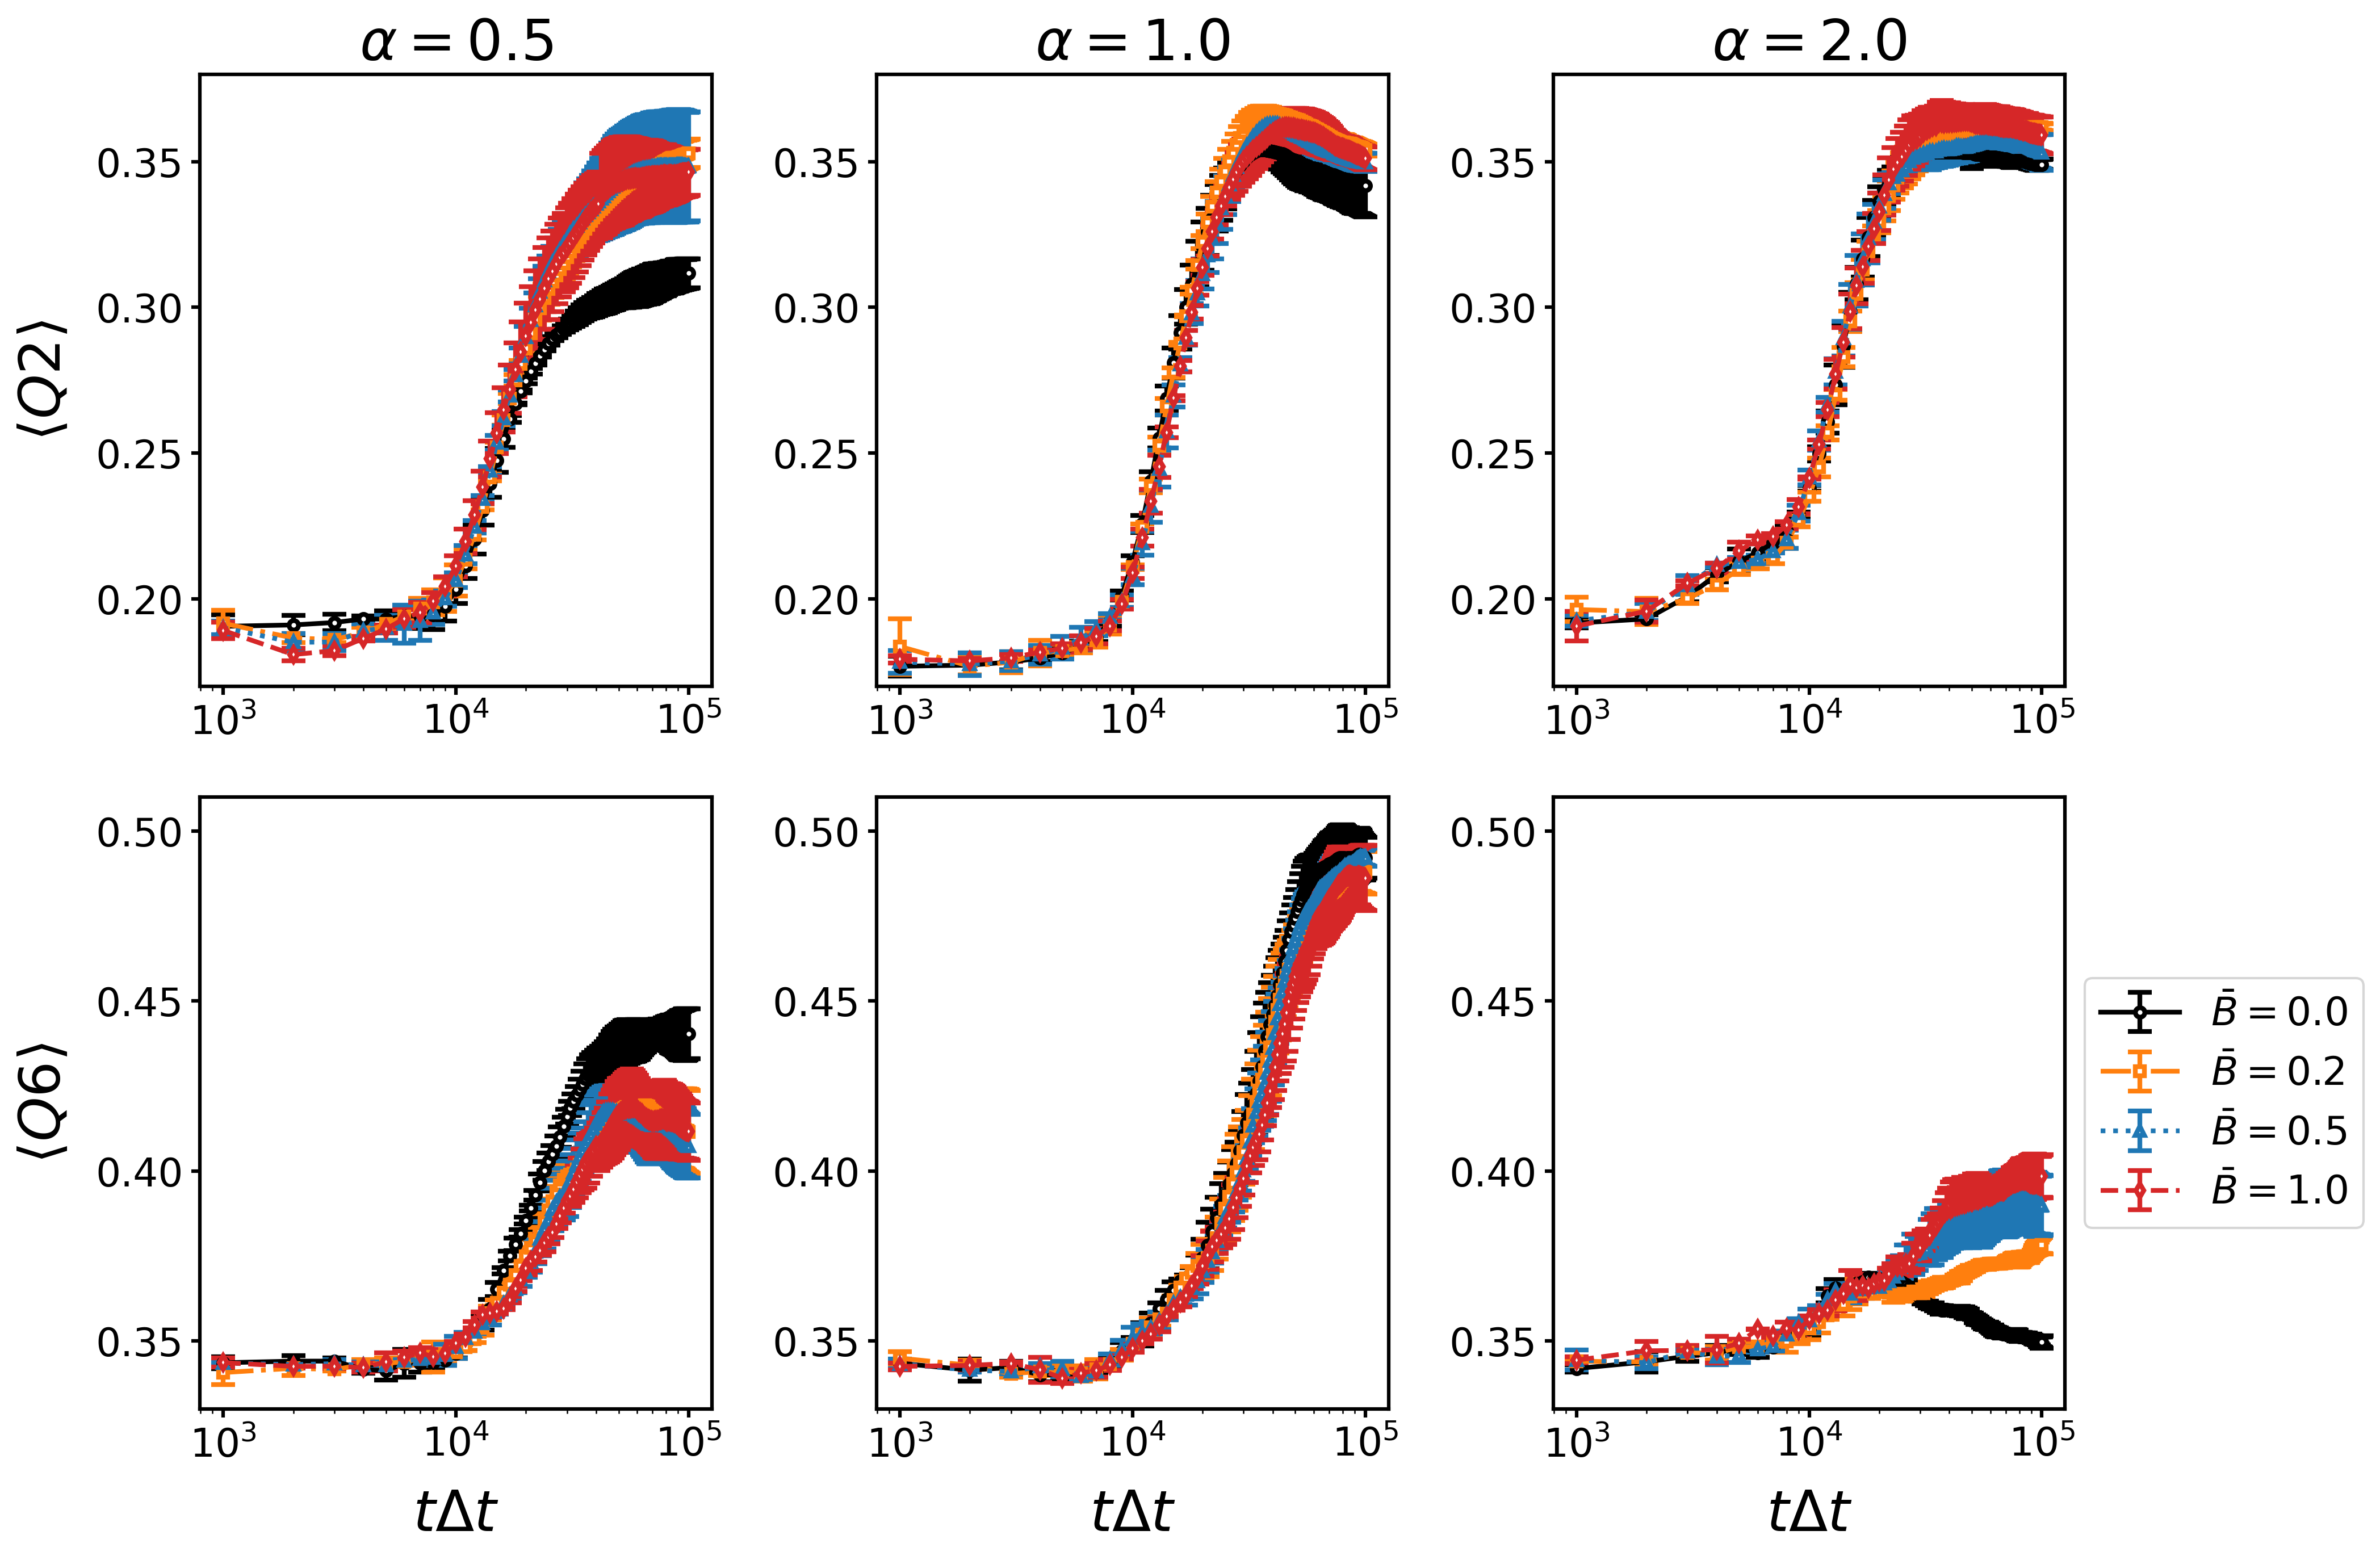
\includegraphics[width=\columnwidth]{figures/results/paper1/steinhardt_vs_coverage.png} 
    \caption{Time dependence of the mean two and six fold symmetry parameter, $\langle Q2 \rangle$ and $\langle Q6 \rangle$ 
    for bijels stabilized with oblate(left), spherical(middle) and prolate(right) particles. I use $\langle Q2 \rangle$ as an
    indicator of global particle translational order while $\langle Q6 \rangle$ is an indicator of local order.} 
    \label{fig:steinhardt_coverage} 
\end{figure}

From Figure \ref{fig:steinhardt_coverage}, I see an increase in disorder in all the bijel systems characterized as an increase in $\langle Q2 \rangle$. 
This is a characteristic of how the particles were initialized and move once the simulation is initiated. The particles are initialized to be randomly placed 
in the simulation domain with roughly equal spacing. As the interface sweeps through the simulation domain, particles irreversibly adsorb onto the interface 
and move with the interface until the bijel jams. I see that $\langle Q2 \rangle$ is magnetic field dependent for oblate particles but not for the spherical 
and prolate particles. I also see an aspect ratio dependence on the values characterized as differences in the time evolution of $\langle Q2 \rangle$. This 
arises due to the differences in the aspect ratio of the particle causing them to arrange differently on the interface as the bijel microstructure evolves.

An increase in $\langle Q6 \rangle$ can indicate an increase in the number of particles adopting icosahedral symmetry at the interface of the amorphous 
interface. \cite{kapfer_jammed_2012} However due to the amorphous nature of the arrangement of particles at the particle monolayer, I use this parameter 
only to gauge changes in local arrangements of particles at the interface and make no commentary on specific interfacial arrangements. For oblate particles, 
I characterize a reduction in local order as the applied field strength is increased, consistent with the increase in $\langle Q2 \rangle$. For prolate 
particles, I observe that $\langle Q6 \rangle$ increases with the applied field. This indicates that the application of the field causes particles to have 
increased local order, even if I see no discernible changes in $\langle Q2 \rangle$. 

The application of the magnetic field affects the prolate and oblate particle differently due to their aspect ratio. At interfaces, rod-like particles 
prefer to orient themselves in an end to end fashion. \cite{eatson_capillary_2023} Disc-like particles have been shown to prefer stacking. \cite{dabat_mesoscale_2018} 
Application of the magnetic field and the presence of an interface will constrain the rotation of the particles, meaning that naturally rods will pack better at 
interfaces than discs as the magnetic field causes the particles to align to the field. This better packing at the interface manifests as greater local ordering 
Next, I analyze how these local toplogical changes affect the microstructure of the bijel by analyzing the channel size distribution of the bijels.

As hypothesized above, the alignment of the particle dipole axis with
the magnetic field reduces the steric constraints within the interface.
To corroborate this idea, I analyzed the radial distribution function
(RDF) of the particles, the calculation of which is detailed in Section
\ref{section:radial_distribution} The time-evolution of the RDFs for the three particle shapes and
varying magnetic flux density is illustrated in Figure \ref{fig:rdf}.

\begin{figure*}
\centering
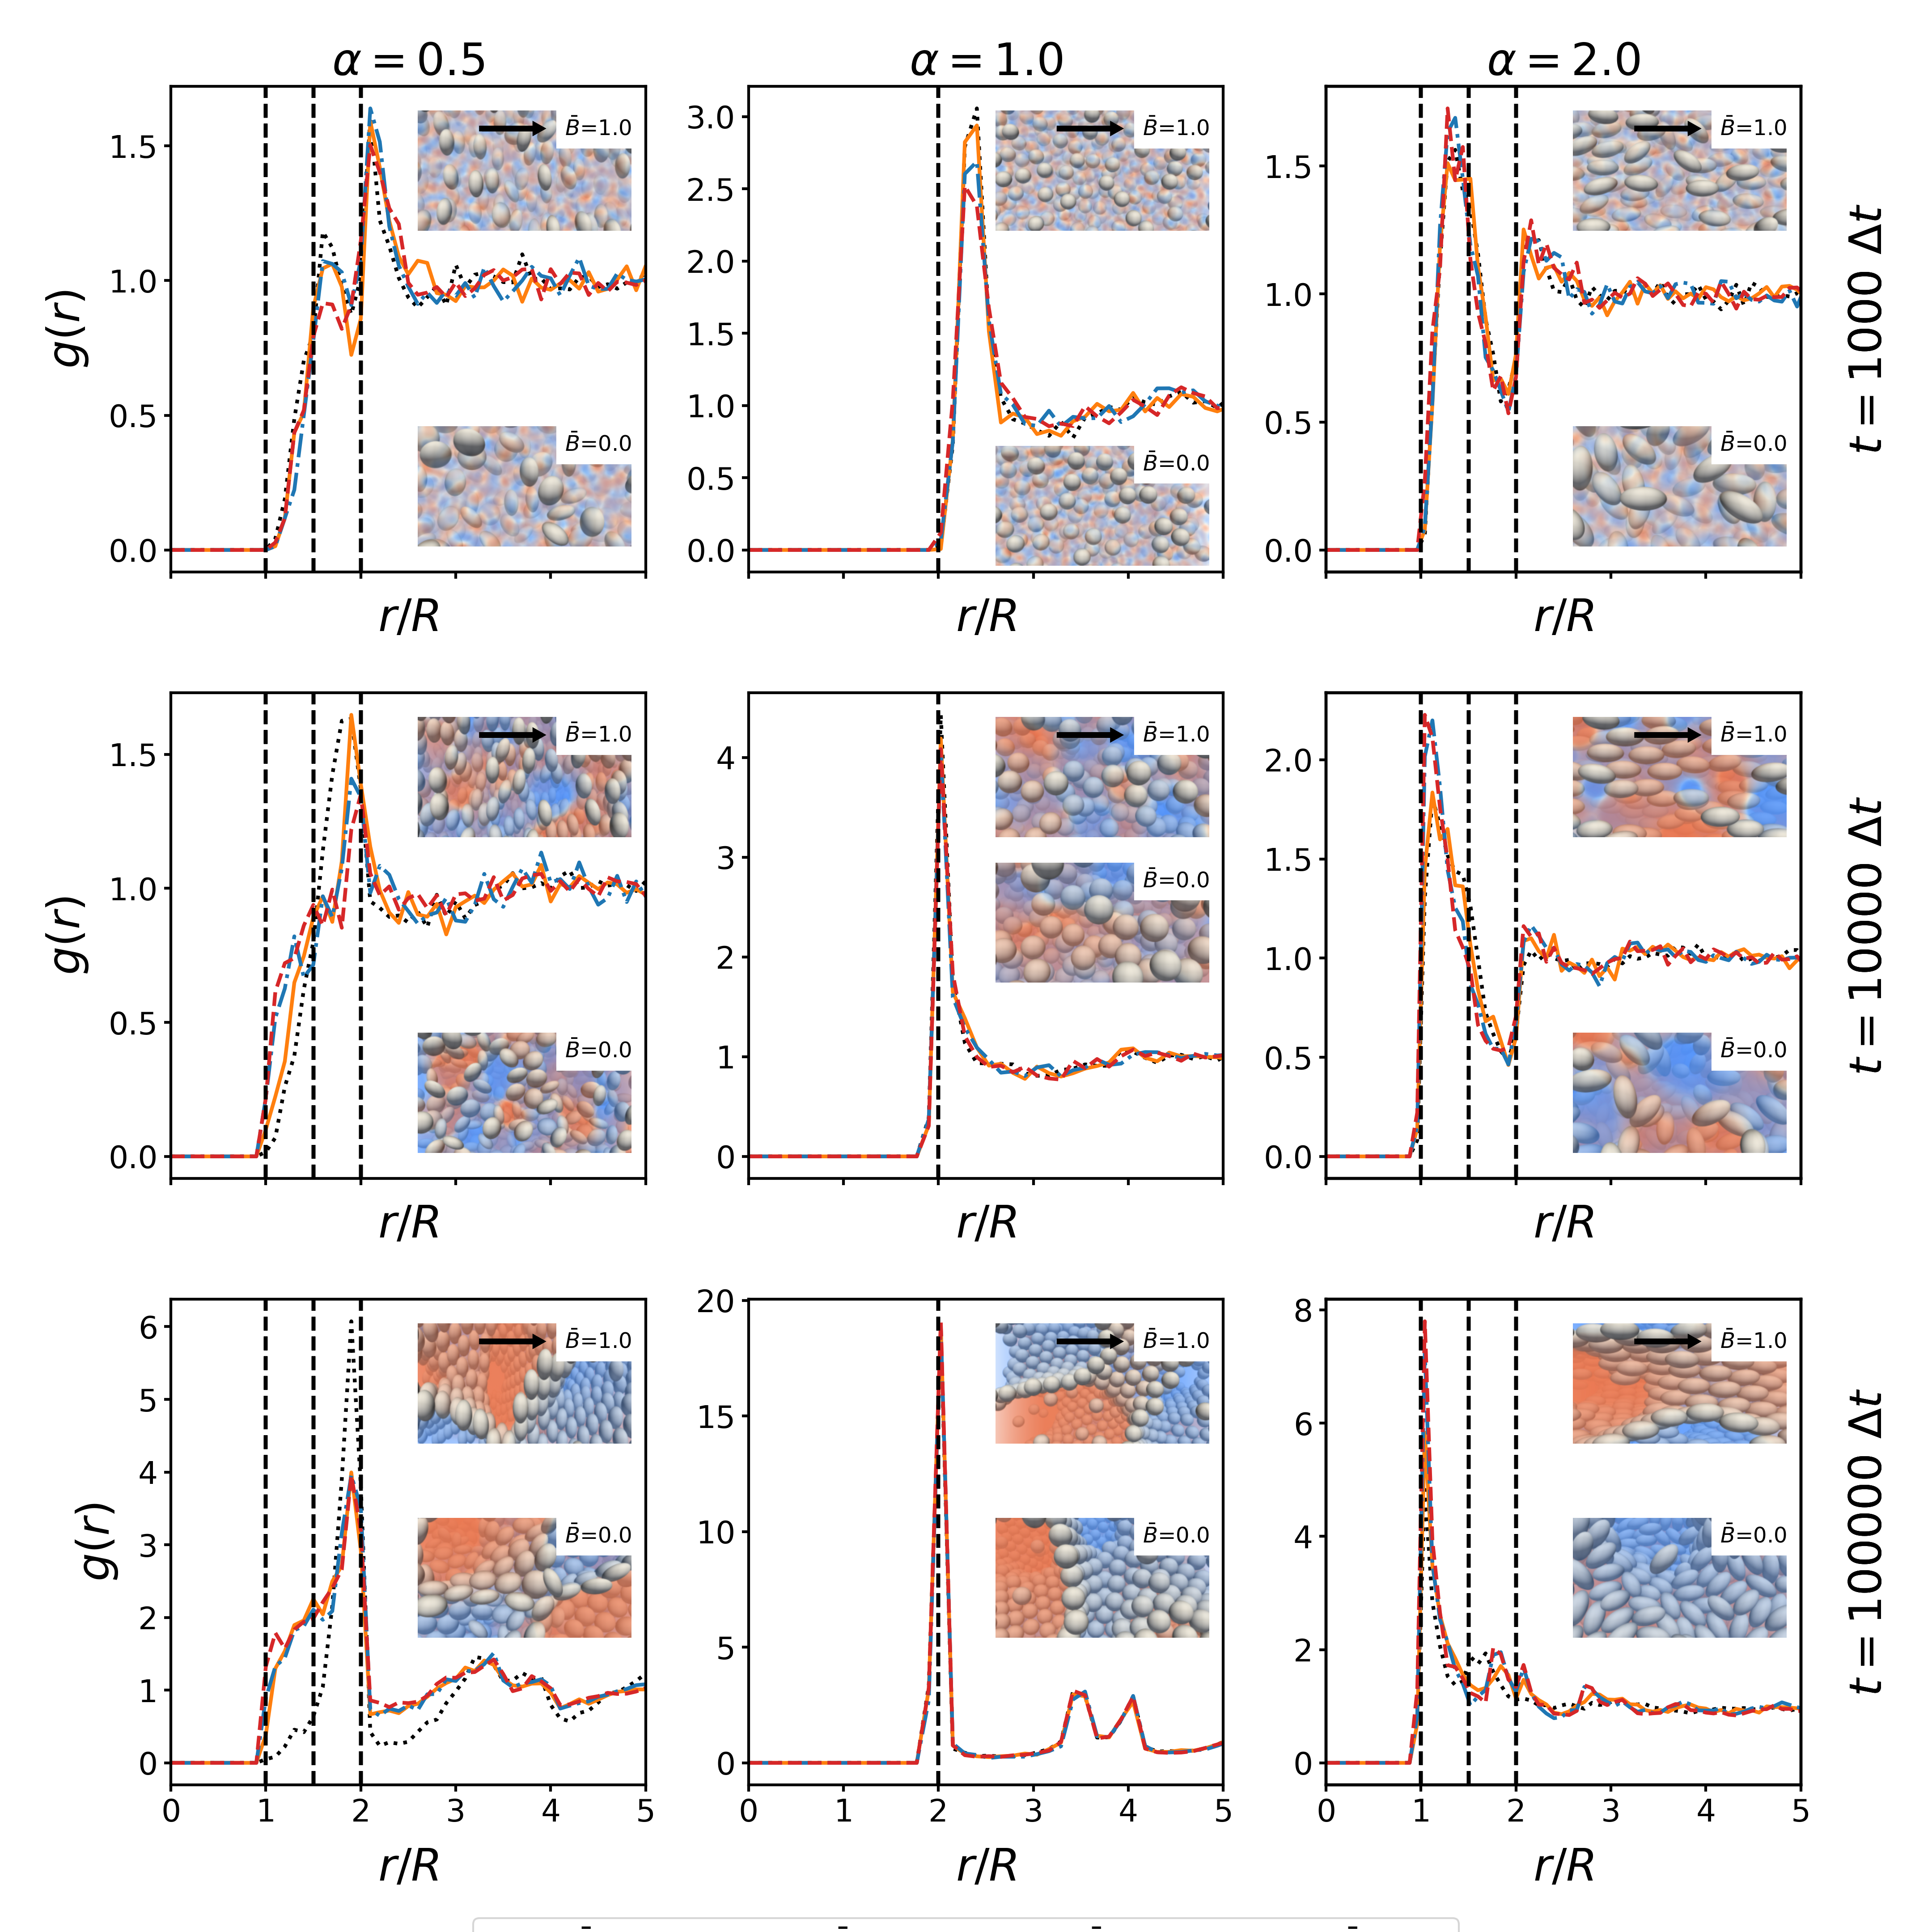
\includegraphics[width=\textwidth]{figures/results/paper1/rdf_compare_time.png}
\caption{Time-evolution of the radial distribution function $g(r)$ of the particles at different magnetic 
        field strength $\bar{B}$. The radial distribution function is shown at $10^3$, $10^4$, and $10^5$ timesteps. 
        The distance $r$ is normalized by the radius $R=\max(R_\parallel,R_\perp)$ of the larger particle axis. The peaks 
        illustrate the packing of particles in the interface. Dashed lines indicate the side-by-side, tip-to-tip, 
        and side-to-tip configuration of particle pairs. For spherical particles, the three values are identical. 
        The insets show snapshots of the particle arrangement with and without magnetic field at the respective timesteps. 
        The direction of the magnetic field is indicated by arrows.}
\label{fig:rdf}
\end{figure*}

The radial distribution function is shown at time steps
\(t=1000\Delta t,\ 10000\Delta t,\ 100000\Delta t\). For ellipsoidal
particles, the characteristic distances between particles in contact are
\(2R_{\parallel}\), \(2R_{\perp}\), and \(R_{\parallel} + R_{\perp}\).
These distances are marked by dashed lines in Fig. \ref{fig:rdf}. We
observe that the largest peak of the RDF coincides with the distance
\(2R_\perp\) for both oblate and spherical particles, indicating that
oblate particles tend to be in contact at their circumference while
prolate particles preferentially align side-by-side. These arrangements
lead to closer packing of particles in the interface. The peaks are less
pronounced in the early stage of the simulations, where the particles
are more randomly oriented. Notably, there is a dip in the RDF of
prolate particles at \(2R_\parallel\) indicating that initially the
tip-to-tip configuration occurs more rarely. The growth of the peak
height over time shows that the magnetic fields promote this alignment
compared to the case without magnetic field. For oblate particles, a
shoulder develops around \(R_\parallel+R_\perp\), indicating that some
particles tilt out of the interface to reduce the covered interfacial
area. For prolate particles, the dip at \(2R_\parallel\) disappears over
time, indicating that more particles align tip-to-tip. This is
consistent with alignment of prolate particles with respect to the
magnetic field, which facilitates closer packing along both axes of the
particles. It further suggests that particles arrange in layers, which can also be observed in the snapshot in Fig.
\ref{fig:packing_viz}. Together with the analysis of nematic order
above, these results substantiate the proposed mechanisms that influence
the formation of bijels with anisotropic particles in magnetic fields:
The magnetic field aligns the particle dipole axis in the field
direction, and the particle re-orientation couples to interface
alignment due to the capillary interactions. The alignment of particles
reduces the steric constraints within the interface, which allows the
interface to shrink further and facilitates domain coarsening. In terms
of the time-evolution, the rotation of particles due to the magnetic
field occurs during the initial stages of the simulation, followed by
the local re-alignment of interfaces due to capillary interactions. In
the case of prolate particles, I observed the shrinking interface can
force particles to tilt out of their preferential alignment to facilitate
closer packing. Generally, our results show that when bijels stabilized
by anisotropic magnetic particles form under the influence of a magnetic
field, the domain size and tortuosity become anisotropic. Additionally,
I observe that the particle packing in the interface becomes more
ordered due to the alignment effects.

\section{Conclusions}

In this work, I studied the effect of applied magnetic fields on the
formation of bijels stabilized by magnetic ellipsoidal particles. We
considered oblate, spherical, and prolate particles with a permanent
magnetic dipole moment suspended in a symmetric binary liquid. I found
that, while the overall formation of a bijel is not disrupted by
magnetic interactions, bijels stabilized by oblate or prolate ellipsoids
exhibit anisotropic domain size and an anisotropic tortuosity. For
oblate particles, the domain size increases in the direction
perpendicular to the magnetic field while the tortuosity increases in
the parallel direction. Conversely, for prolate particles, the domain
size increases in the direction parallel to the magnetic field while the
tortuosity increases in the perpendicular direction. Compared with
bijels formed in the absence of a magnetic field, I observed changes in
domain size up to \(30\%\) for non-spherical particles. This effect can
be explained by the re-orientation of the particle dipole axis with the
magnetic field, which in turn re-aligns the interfaces in the direction
of the longer axis of the particles. I further corroborated this
mechanisms by analyzing the coarsening speed and the nematic order of
the particles and the interfaces. I found that jamming of particles is
delayed in the direction of the longer ellipsoidal axis leading to
enhanced coarsening in this direction. The timescale of the delayed
jamming coincides with a slow-down of the orientational ordering of the
particles whereas the alignment of the interfaces increases. I also
found that the angle between the particle dipole axis and the interface
normal changes at this stage. Additionally, I analyzed the radial
distribution function of the particles and found that prolate particles
tend to align side by side, while the oblate particles exhibit a less
regular arrangement. Based on these findings, I propose that bijel
formation in magnetic fields is governed by two coupled effects: During
the initial stage, the magnetic torque rotates the particles to align
the magnetic dipole moment with the field, and the orientational order
of the particles facilitates further coarsening. As coarsening proceeds,
the capillary interactions cause the interfaces to align with the longer
particle axis. The shrinking interface compresses the particles into
ordered arrangements. When jamming sets in, some particles can be forced
to tilt out of the interface and this effect is more prominent for
oblate particles.

Our results demonstrate the effects of magnetic fields on the structural
properties of bijels stabilized by ellipsoidal magnetic particles. This
control is desirable in applications where the domain size and
tortuosity affect the transport properties. For example, reduced
tortuosity can increase the diffusive permeability of bone-like
materials \cite{prakoso2023tortuosity}. Similarly, low tortuosity
in lithium electrodes facilitates homogeneous ion transport and
uniform lithium deposition, leading to enhanced cyclability of
batteries\cite{chen_tortuosity_2020, ebner_tortuosity_2014}. Whereas we
have considered one particular regime of spinodal decomposition, the
viscosity and surface tension of the liquids offer additional parameters
that could be leveraged to tune the bijel formation. Moreover, the
particle volume fraction is another parameter that is known to affect
the formation of particle-stabilized emulsions
\cite{jansen_bijels_2011,hijnen_bijels_2015}. With respect to possible
experimental realizations of our simulations, I should emphasize that
I have generally considered micron-size particles and have neglected
thermal fluctuations. At the nanoscale, thermal fluctuations may in
principle play a role, however, Reeves et
al.~\cite{reeves_particle-size_2015} have shown that nanoparticles
benefit from smaller driving forces towards disruptive curvature and
actually lead to more robust bijel formation. Nevertheless, the
stability of magnetically-responsive bijels is a relevant question for
applications that involve shear flows such as crossflow reactors
\cite{khan_nanostructured_2022}. Aside from particle-size and shape
effects, direct interactions between particles are a possible avenue
to tune the formation of particle-stabilized emulsions gels, as the
recent discovery of bicontinuous intraphase jammed emulsion gels
(bipjels) illustrates \cite{kinkead_bicontinuous_2019}. Another
interesting observation arising from our simulations is that the
packing order of particles in the interface appears to increase when
bijels form under the influence of a magnetic field. While such
interfacial ordering effects have been studied on planar interfaces
\cite{toor_self-assembly_2016,shi_nanoparticle_2018,kim_dynamic_2022},
they have hitherto not been reported for particle-stabilized emulsion
gels. It would be interesting to examine the implications of this
ordering on the optical and transport properties of jammed emulsion
gels. In conclusion, our simulations provide relevant insights into the
formation of magnetic particle-stabilized bijels in the presence of
external magnetic fields, and they demonstrate the potential of magnetic
particles for fabrication of emulsion systems with tunable and
anisotropic particle packing and domain structure.

\chapter{Structural response of bijels under magnetic fields}

\section[Introduction]{Introduction\protect\footnote{Sections of this chapter appear in a manuscript submitted to Springerlink as part of the International Conference on Computational 
Science (ICCS) 2025 in the Computing and Data Science for Materials Discovery and Design track, submission number 259 and is
reproduced with permission of Palgrave Springer Nature.}}

% [author and/or editor(s) of contribution], [volume and/or contribution title], [year of publication], [publisher (as it appears on our copyright page)] \

Emulsions can adopt a variety of microstructures depending on fluid volume fractions and the affinity of stabilizing agents for each phase. Among these, bicontinuous 
interfacially jammed emulsion gels (bijels) are characterized by a tortuous, co-continuous network of immiscible fluid domains stabilized by colloidal particles. This 
unique architecture lends itself to numerous advanced applications, including membrane fabrication, catalyst supports, battery electrodes, and pharmaceutical delivery 
systems. Bijels form through the arrest of spinodal decomposition in partially miscible fluid mixtures: as phase separation proceeds, the interface sweeps through the 
system, adsorbing particles until the interfacial area becomes saturated, resulting in jamming. Microstructural features such as domain size, continuity, and interfacial 
curvature critically influence material performance, affecting properties like mass transport, mechanical stability, and surface reactivity. Since their discovery via 
simulation and subsequent experimental realization, research on bijels has expanded significantly, exploring diverse synthesis conditions and scalable processing methods.

The functional properties of bijels are inherently linked to their internal structure. For instance, lower tortuosities in the direction of ion transport yield improved charge 
rates and cycling stability in battery electrodes \cite{ebner_tortuosity_2014, samdani_bicontinuous_2017}. In liquid-liquid extraction, the characteristic pore length-scale governs 
molecular selectivity \cite{khan_nanostructured_2022}, while in pharmaceutical applications, domain size influences drug release rates and cellular behavior 
\cite{vanoli_bijels_2022, thorson_bijel-templated_2019}. Given the sensitivity of these properties to microstructural characteristics, the ability to dynamically modify bijel 
morphology presents a promising strategy to adapt their behavior in situ for targeted performance. In this context, stimuli-responsive emulsions have garnered increasing interest 
for applications requiring dynamic control over material properties, such as enhanced oil recovery, reaction separation, and therapeutic delivery 
\cite{tham_magnetophoresis_2021, cui_stabilizing_2013, rozynek_opening_2019, lu_controllable_2020}. 

These systems can be operated by using external stimuli to alter interfacial configurations, 
enabling modulation of permeability, interfacial area, and morphology. For example, in emulsions stabilized by spherical particles, electric fields can induce droplet deformation via 
particle unjamming and migration before re-establishing interfacial jamming \cite{cui_stabilizing_2013}. Among various stimuli, magnetic fields are particularly attractive due to their 
remote addressability, material compatibility, and bio-relevance. Core-shell ferrite-hydroxyapatite nanorods, for instance, exhibit reversible morphological changes depending on initial 
particle orientation and field direction \cite{nakayama_stimuli-responsive_2018}. In magnetically stabilized Pickering emulsions, magnetophoresis has been shown to drive particle migration 
and interfacial distortion or collapse \cite{tham_magnetophoresis_2021, yang_rapid_2020, misra_magnetic_2020}. Chapter 4 demonstrated that magnetic fields applied during bijel formation can 
bias domain coarsening, producing anisotropic microstructures via orientation-specific jamming \cite{karthikeyan_formation_2024}. However, the structural response of bijels to magnetic fields 
after formation remains poorly understood, presenting an opportunity to explore how external fields may be used to dynamically reconfigure established bijel architectures.

This study investigates the post-formation structural response of bijels stabilized by ellipsoidal magnetic particles under the influence of externally applied magnetic fields. 
Using a hybrid Lattice Boltzmann Method coupled with Molecular Dynamics, we simulate the formation and evolution of bijel structures stabilized by rod-like particles modeled as 
magnetic dipoles. We find that increasing the applied magnetic field after formation induces microstructural changes characterized by increased domain anisotropy and 
coarsening, up to a saturation threshold. In contrast, decreasing or removing the magnetic field results in minimal morphological change, suggesting that the structure is
resilient to removal of stimuli. Analysis reveals that particle unjamming, reorientation at the interface, and subsequent re-jamming are responsible for these structural transformations.
These findings demonstrate how magnetic field manipulation, in combination with ellipsoidal particle stabilization, enables tunable, on-demand microstructure 
control in bijels, offering new capabilities for adaptive material design.

% To understand the saturation behavior, we applied magnetic fields of varying strength to bijel templates formed under increasing initial field conditions. We observed that 
% a greater initial nematic order parameter negatively correlated with the extent of microstructure change. Finally, switching off the magnetic field in pre-aligned bijels had little 
% impact on the microstructure, indicating that the jammed interfacial network prevents reversal of anisotropic features. 

\section{Results}
% \section[Results]{Introduction\protect\footnote{Sections of this chapter appear in a manuscript submitted to Springerlink as part of the International Conference on Computational 
% Science (ICCS) 2025 in the Computing and Data Science for Materials Discovery and Design track, submission number 259 and is
% reproduced with permission of Palgrave Springer Nature.}}
% \label{sec:results_p2}

\subsection{Kinetic arrest}
\label{section:hysteresis_curve}

Bijels have proposed applications as soft-matter-based material templates, drug delivery vectors, and separation systems. In all cases, material performance is 
tightly coupled to the internal microstructure of the bijel template. Applications that benefit from adaptive permeability or structural tunability would be 
enhanced by the ability to reversibly modulate microstructure in situ. This section explores whether magnetically responsive bijels can undergo reversible 
structural changes upon repeated application and removal of an external magnetic field.

We begin by analyzing bijels stabilized by prolate ellipsoidal particles at a particle volume fraction of \(\phi_p = 0.1\). This system is selected due to the 
similar qualitative response mechanisms observed for both prolate and oblate geometries in preliminary simulations (Aim 1), with prolate particles chosen here 
for their greater experimental accessibility. The bijel is initially formed without a magnetic field. After equilibration, a static magnetic field is applied 
in the \(z\)-direction and incrementally increased: \(\bar{B}_z = 0 \rightarrow 0.2 \rightarrow 0.5 \rightarrow 1\). This is followed by a symmetric 
decrement: \(\bar{B}_z = 1 \rightarrow 0.5 \rightarrow 0.2 \rightarrow 0\). At each step, the system is allowed to evolve to a new equilibrium, defined as
the plateauing of the length scale obtained from the domain size, \(L\), computed from the first moment of the spherically averaged structure factor.
\cite{kendon_3d_1999,kendon_inertial_2001} The procedure for the domain size can be found in Equation \ref{eq:spherically_averaged_structure_factor}.

The hysteresis behavior is shown in Figure~\ref{fig:hysteresis_curve}, which plots the normalized domain size \(L/R\) as a function of the applied magnetic 
field at the end of the equilibration step.

\begin{figure} 
    \centering 
    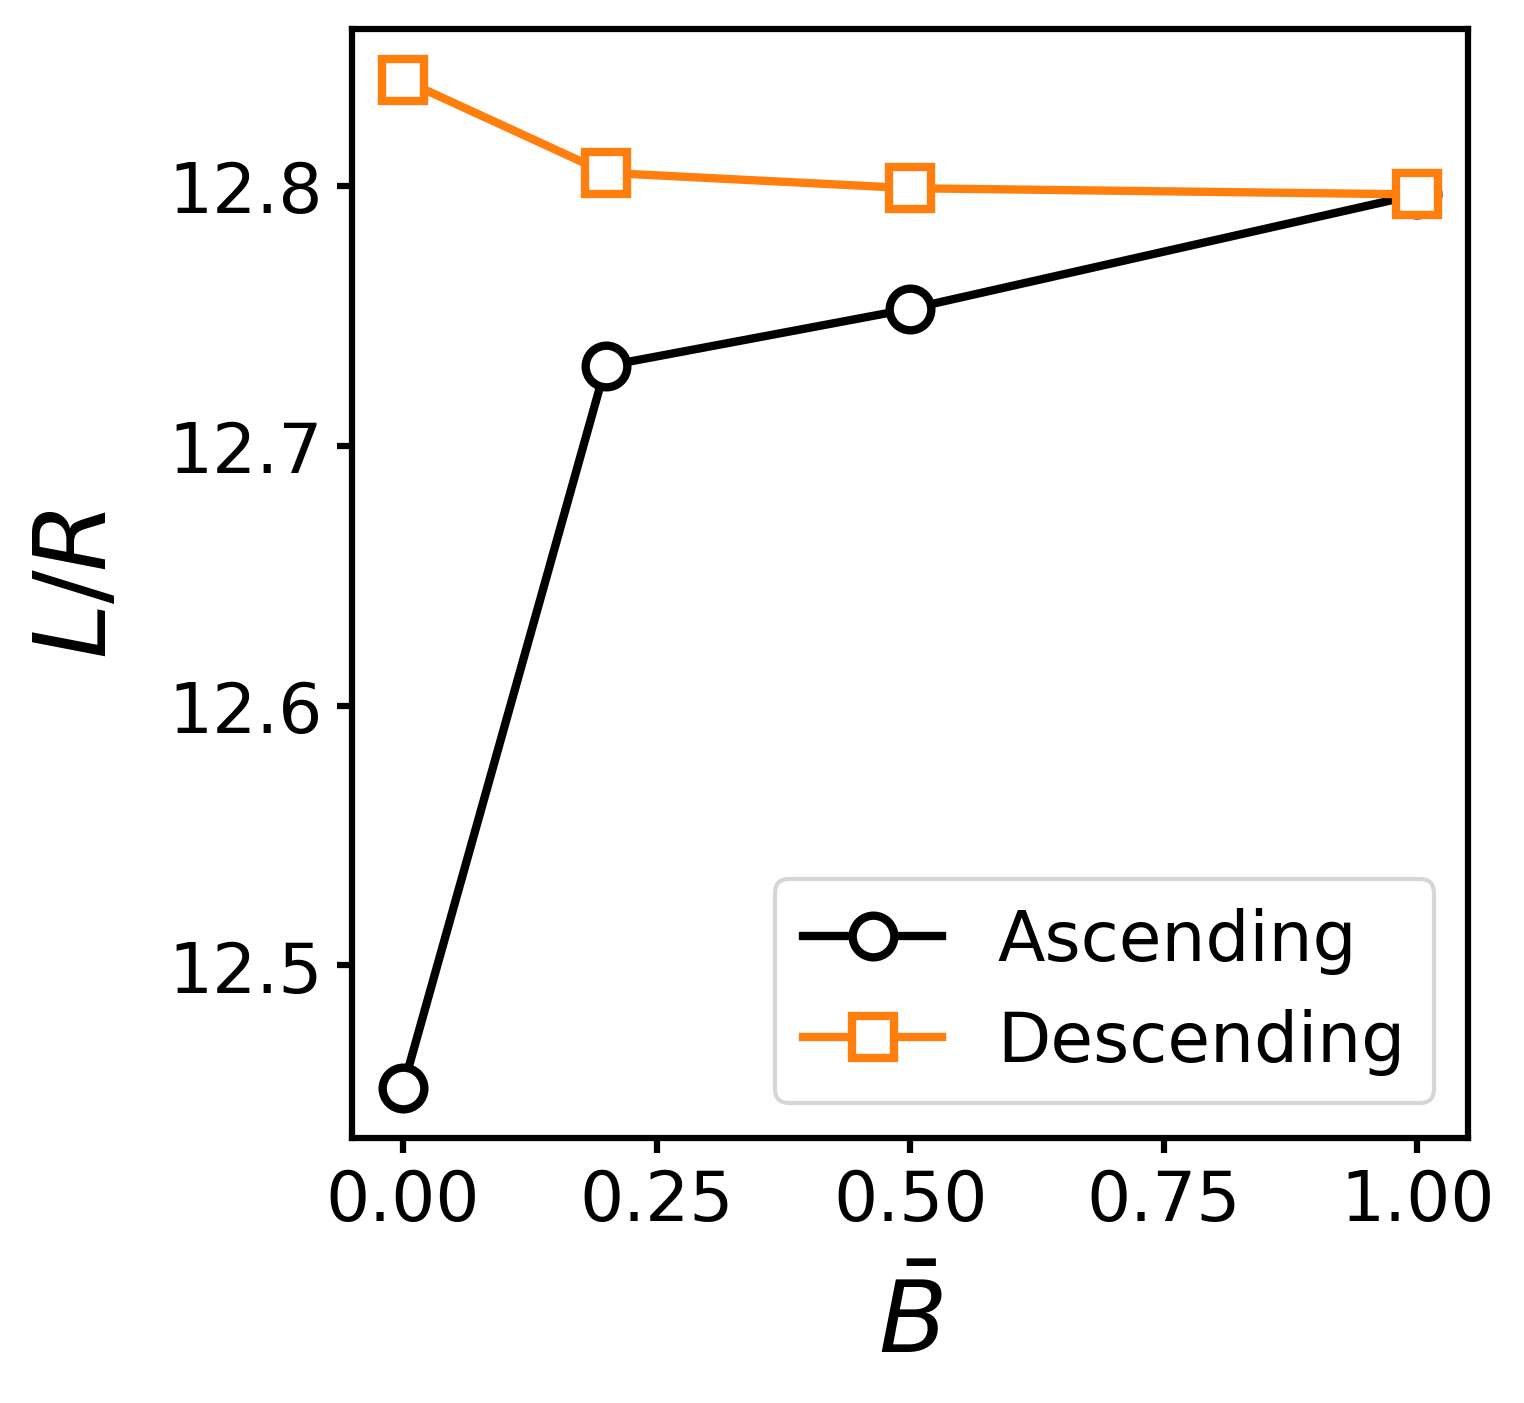
\includegraphics[scale=0.5]{../figures/results/paper2/hysteresis_curve.png} 
    \caption{Plot of the domain size of a bijel stabilized by magnetically responsive prolate particles. We observe that the domain size increases as we 
    increase the applied magnetic field strength. However, upon decrease of the applied field strength the microstructure does not return to its previous value,
    demonstrating kinetic arrest.} 
    \label{fig:hysteresis_curve} 
\end{figure}

The domain sizes characterized in Figure~\ref{fig:hysteresis_curve} demonstrates that as the field is increased, domain size increases, indicating coarsening 
of the fluid domains in the bijel. Chapter 4 showed that application of magnetic fields cause reordering of particles at interfaces towards the
direction of the applied field, enforcing nematic order in the particle monolayer. In the case of already formed bijels,
this reorientation reduces the interface area stabilized, facilitating local unjamming and domain growth. In contrast, when the field strength is reduced, 
the domain size does not revert to its original value, suggesting that the microstructure remains kinetically arrested in the coarsened configuration.

A similar phenomenon has been reported by Cui et al.~\cite{cui_stabilizing_2013} in studies of particle-stabilized emulsions subjected to electric fields, 
where spherical particles unjammed and subsequently rejammed in a new configuration, resulting in anisotropic droplet deformation. Our results extend this 
concept to jammed, bicontinuous systems stabilized by anisotropic particles. Notably, Figure~\ref{fig:hysteresis_curve} also shows that the degree of 
structural change is field-strength dependent, indicating that stronger fields drive more extensive particle reconfiguration. In the following sections, 
we investigate how the magnitude of the applied field and the initial degree of particle ordering influence the extent and reversibility of microstructural 
evolution in magnetically responsive bijels.

\subsection{Applying a field onto a bijel with disordered particles}
\subsubsection{Field strength dependence on domain size}
\label{section:field-strength-dependence-on-domain-size}

The results presented in Figure~\ref{fig:hysteresis_curve} demonstrate that changes in bijel domain size are dependent on the strength of the applied magnetic 
field. in many proposed stimuli-responsive applications, understanding not only the extent but also the mechanism
of structural response is critical for functionality and control. In this section, we investigate the dynamic structural response of bijels stabilized by randomly 
oriented ellipsoidal particles with a volume fraction of \(\phi_p = 0.1\), initially formed without a magnetic field. Magnetic fields of varying strengths 
(\(\bar{B} = 0, 0.2, 0.5, 1\)) are applied to these pre-formed structures to assess how the microstructure evolves under external stimuli. We begin by visualizing 
the microstructure of bijels stabilized by prolate particles before and after field application.

\begin{figure} 
\centering 
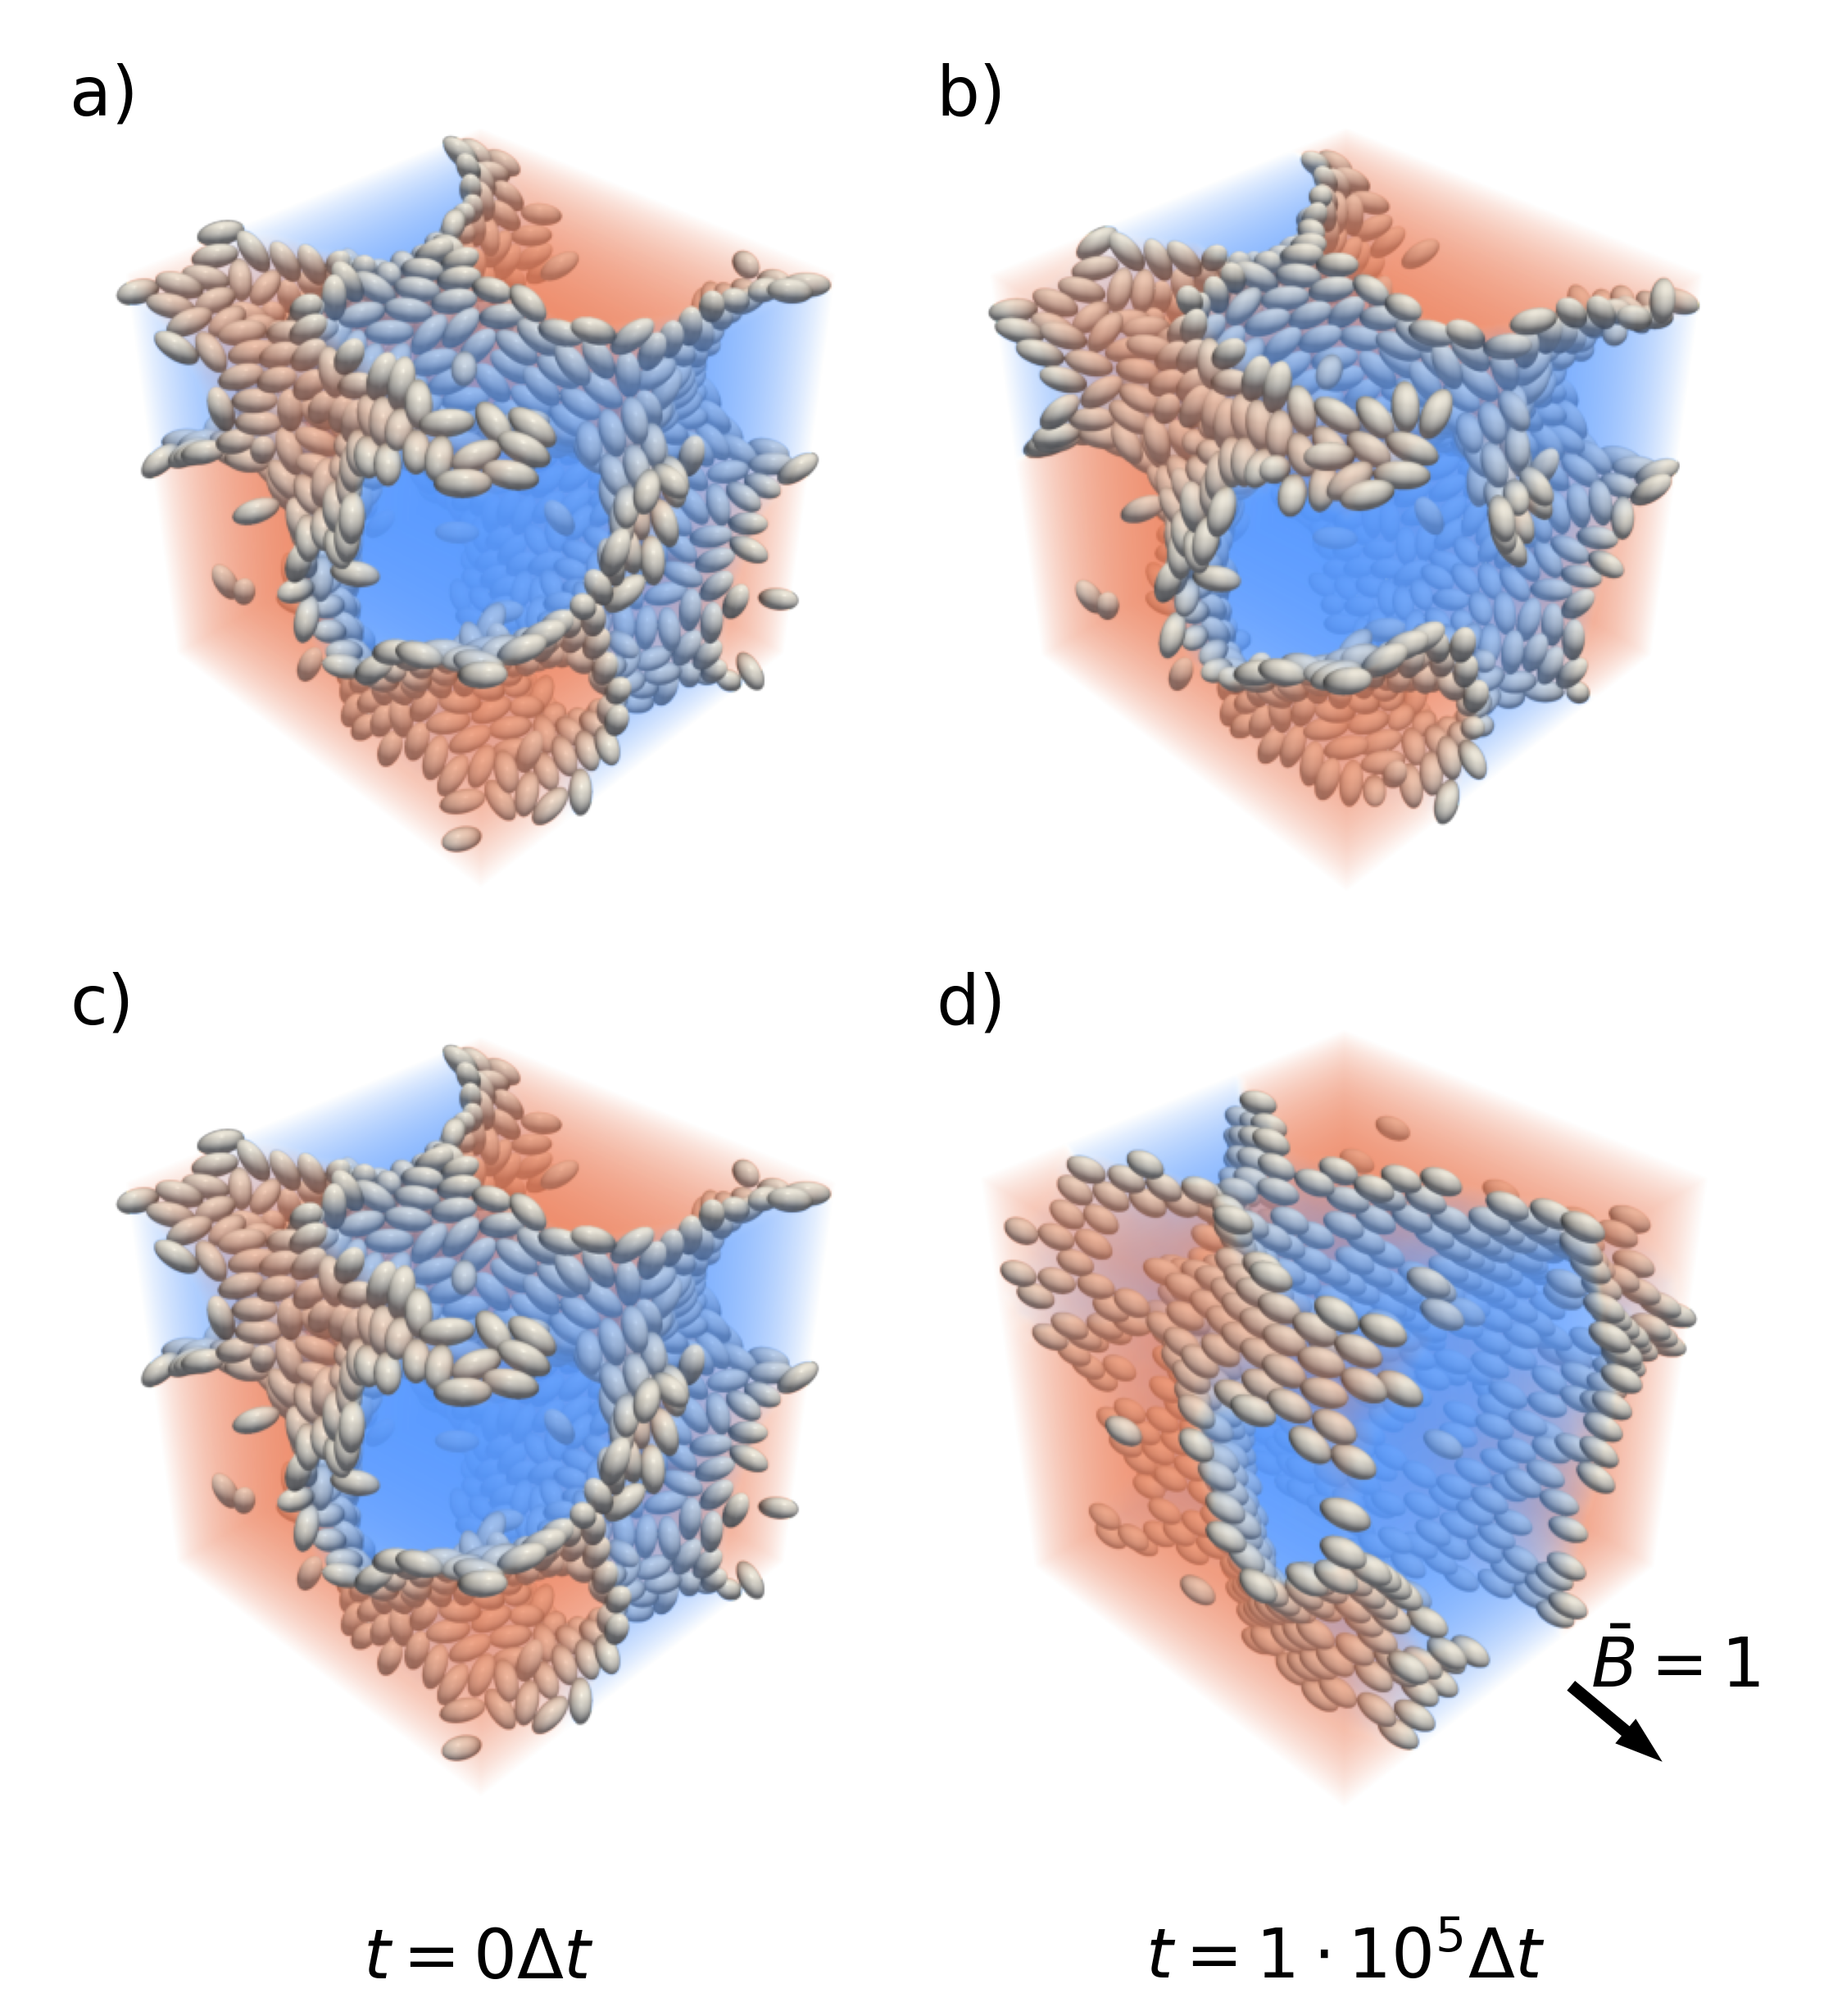
\includegraphics[scale=0.5]{../figures/results/paper2/microstructure_viz-field_on.png} 
\caption{Visualizations of bijels stabilized by prolate particles simulated under no fields at $t = 0$ (left columns) and $t = 10^5$ (right columns). The top 
         row detail the microstructure evolution for bijels with no applied field while the bottom rows show bijels stabilized by oblate and prolate particles 
         respectively with a field strength of $\bar{B} = 1$ applied.}
\label{fig:microstructure_viz-field_on} 
\end{figure}

Figure~\ref{fig:microstructure_viz-field_on} shows that at zero field, the fluid domains exhibit an isotropic, co-continuous morphology with particles randomly 
distributed and oriented at the fluid interface. Upon applying a magnetic field (\(\bar{B}_z = 1\)), the particles undergo reorientation along the field direction, 
which visibly alters the interfacial configuration and the domain morphology. 
To quantitatively characterize this response, we compute the average domain size as a function of time and magnetic field strength. 

\begin{figure} 
    \centering 
    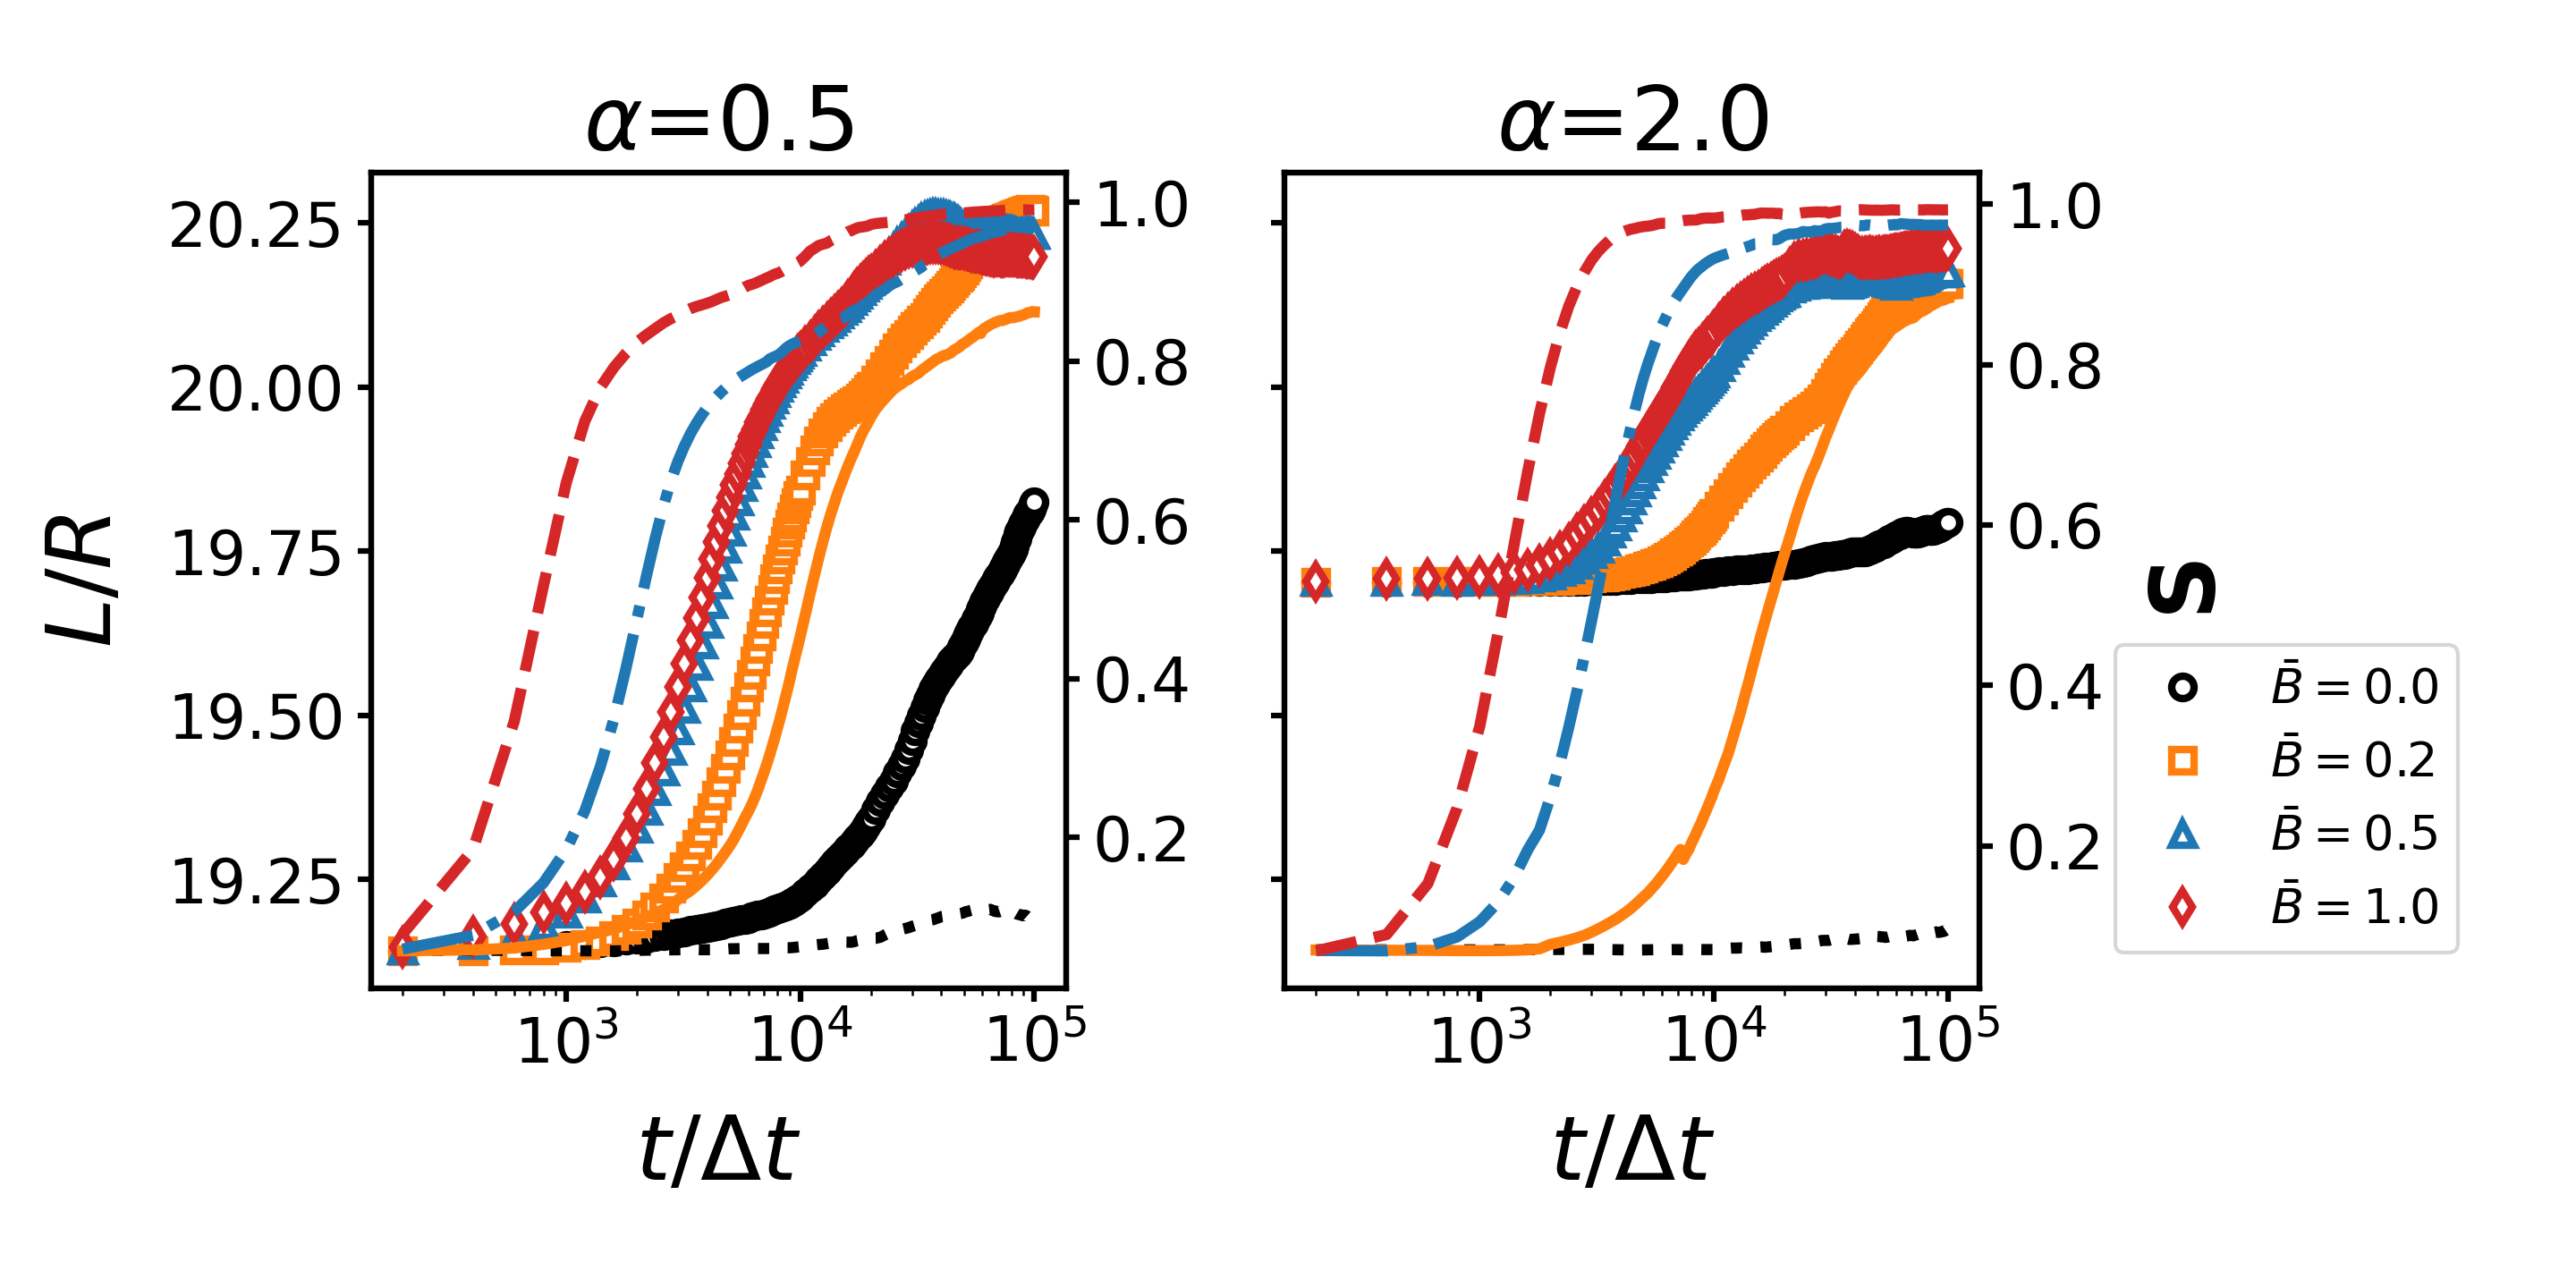
\includegraphics[scale=0.6]{../figures/results/paper2/domain_size-field_on.png} 
    \caption{Plots of the time evolution of the normalized domain size \(L/R\) (markers) for bijels stabilized by oblate (left, \(\alpha = 0.5\)) 
             and prolate (right, \(\alpha = 2.0\)) ellipsoidal particles under varying magnetic field strengths. Here, \(R = 7.9\) is the volume-equivalent sphere radius.} 
    \label{fig:domain_size-field_on} 
\end{figure}

The results show that applying a magnetic field to bijels 
initially formed without one induces domain coarsening, with the final domain size increasing by up to 5.2\% for oblate and 2.5\% for 
prolate particle-stabilized systems.
In both oblate and prolate systems, domain coarsening follows a characteristic three-stage evolution: an initial slow growth phase, a period of rapid 
coarsening, and eventual plateauing as the structure reaches a new jammed configuration. Even in the absence of a magnetic field (\(\bar{B}_z = 0\)), 
domain growth is observed driven by steric rearrangement of interfacial particles, consistent 
with findings by Günther et al.~\cite{gunther_timescales_2014}. 

In Chapter 4, it was identified that the microstructure became anisotropic upon application of magnetic fields. To characterize if the same is observed
when applying a magnetic field onto a formed bijel, we plot the anisotropic domain size and tortuosity as a function of the applied magnetic field. The
directional domain size is calculated using the technique outlined in Equation \ref{eq:directional_structure_factor} and the tortuosity is calculated
using the technique used to generate the data for Figure \ref{fig:tau_B}.

\begin{figure} 
    \centering 
    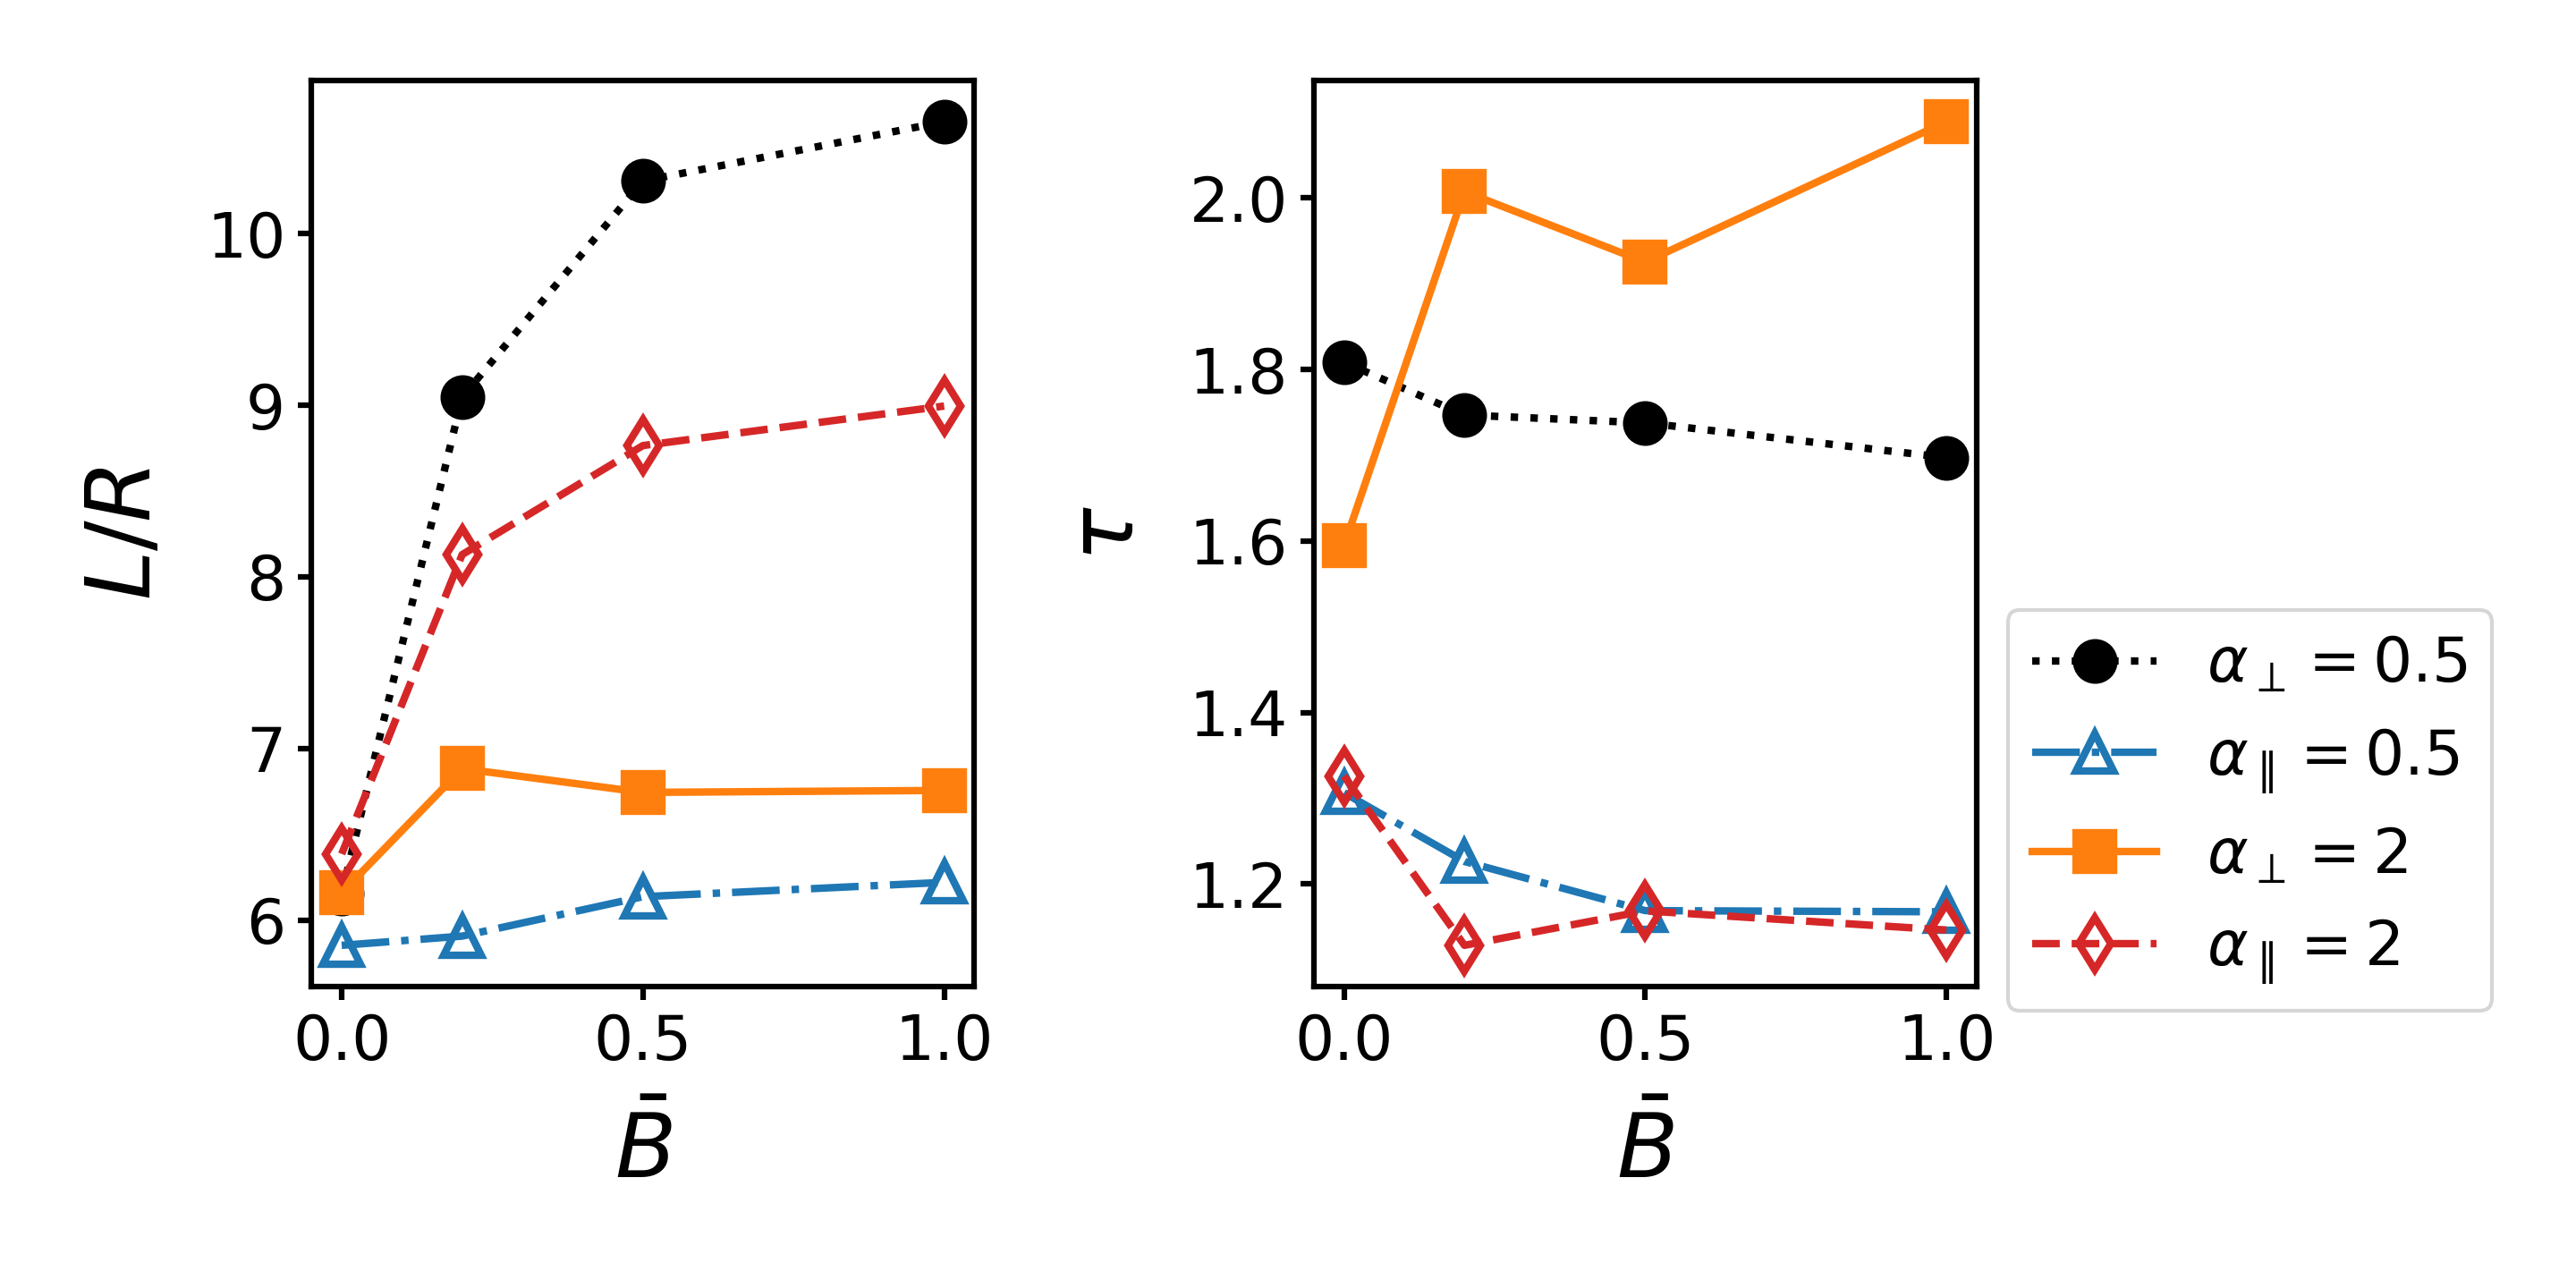
\includegraphics[scale=0.6]{../figures/results/paper2/domain_size_aniso-field_on.png} 
    \caption{Plots of the anisotropic domain size (left) and tortuosity (right) as a function of magnetic field strength for bijels 
             stabilized with oblate and prolate ellipsoids when raising the applied magnetic field. Prolate-stabilized bijels 
             exhibit increased domain size parallel to the field ($L_{\parallel}$) and decreased size perpendicular ($L_{\perp}$), 
             while the opposite trend is observed for oblate-stabilized systems. Tortuosity inversely correlates with domain size in 
             both cases.} 
    \label{fig:domain_size_aniso-field_on} 
\end{figure}

Figure~\ref{fig:domain_size_aniso-field_on} shows that the application of a magnetic field induces domain size anisotropy in bijels stabilized by both oblate 
and prolate particles. Even at zero field, a small degree of anisotropy is observed, which increases substantially with rising field strength. For oblate particles, 
the domain sizes perpendicular (\(L_\perp\)) and parallel (\(L_\parallel\)) to the applied field increase by approximately 73\% and 7\%, respectively. In contrast, 
for prolate particles, \(L_\perp\) increases by 10\%, while \(L_\parallel\) increases by 44\%. These results indicate that the dominant direction of coarsening 
depends on particle morphology: oblate particles promote greater coarsening perpendicular to the field, while prolate particles favor coarsening parallel to the 
field. This trend reflects how particles reorient in response to the applied magnetic field. As particles unjam and rejam 
at the interface, they adopt morphology- and field-dependent orientations that result in directionally biased surface coverage, manifesting as anisotropic domain 
growth.

The right panel of Figure~\ref{fig:domain_size_aniso-field_on} presents the corresponding changes in directional tortuosity. Initially, the tortuosity values 
for both directions are close to \(\tau \approx 1.5\), aligning with previous simulations of gyroidal and co-continuous structures using Lattice Boltzmann methods 
\cite{luo_macroscopic_2020}. Upon applying the magnetic field, \(\tau_\perp\) decreases while \(\tau_\parallel\) increases. This inverse relationship between 
tortuosity and domain size is consistent with prior findings \cite{karthikeyan_formation_2024}, where larger domains exhibited 
reduced tortuosity. The observed anisotropic response suggests that magnetic fields not only influence interfacial particle orientation but also lead to 
direction-dependent transport pathways in the bijel. Moreover, the extent and direction of anisotropy are strongly influenced by the particle morphology, 
particularly the axis of symmetry, which dictates the dominant direction of microstructural reorganization under field application. The time dependence of
the reorientation of particles at the interface is characterized next.

\subsubsection{Particle reorientation at the interface}

The primary effect of the magnetic field is the torque it exerts on the particles' magnetic dipoles, driving them to rotate and align with the field direction. 
This field-induced alignment is clearly evident in the simulation snapshots shown in Figure~\ref{fig:particle_viz-field_on}. In the absence of a magnetic field 
(\(\bar{B} = 0\)), the particles exhibit random orientations at the interface. However, when the field is applied (\(\bar{B} = 1\)), the dipoles display a strong 
degree of orientational order aligned with the field direction.

\begin{figure} 
\centering 
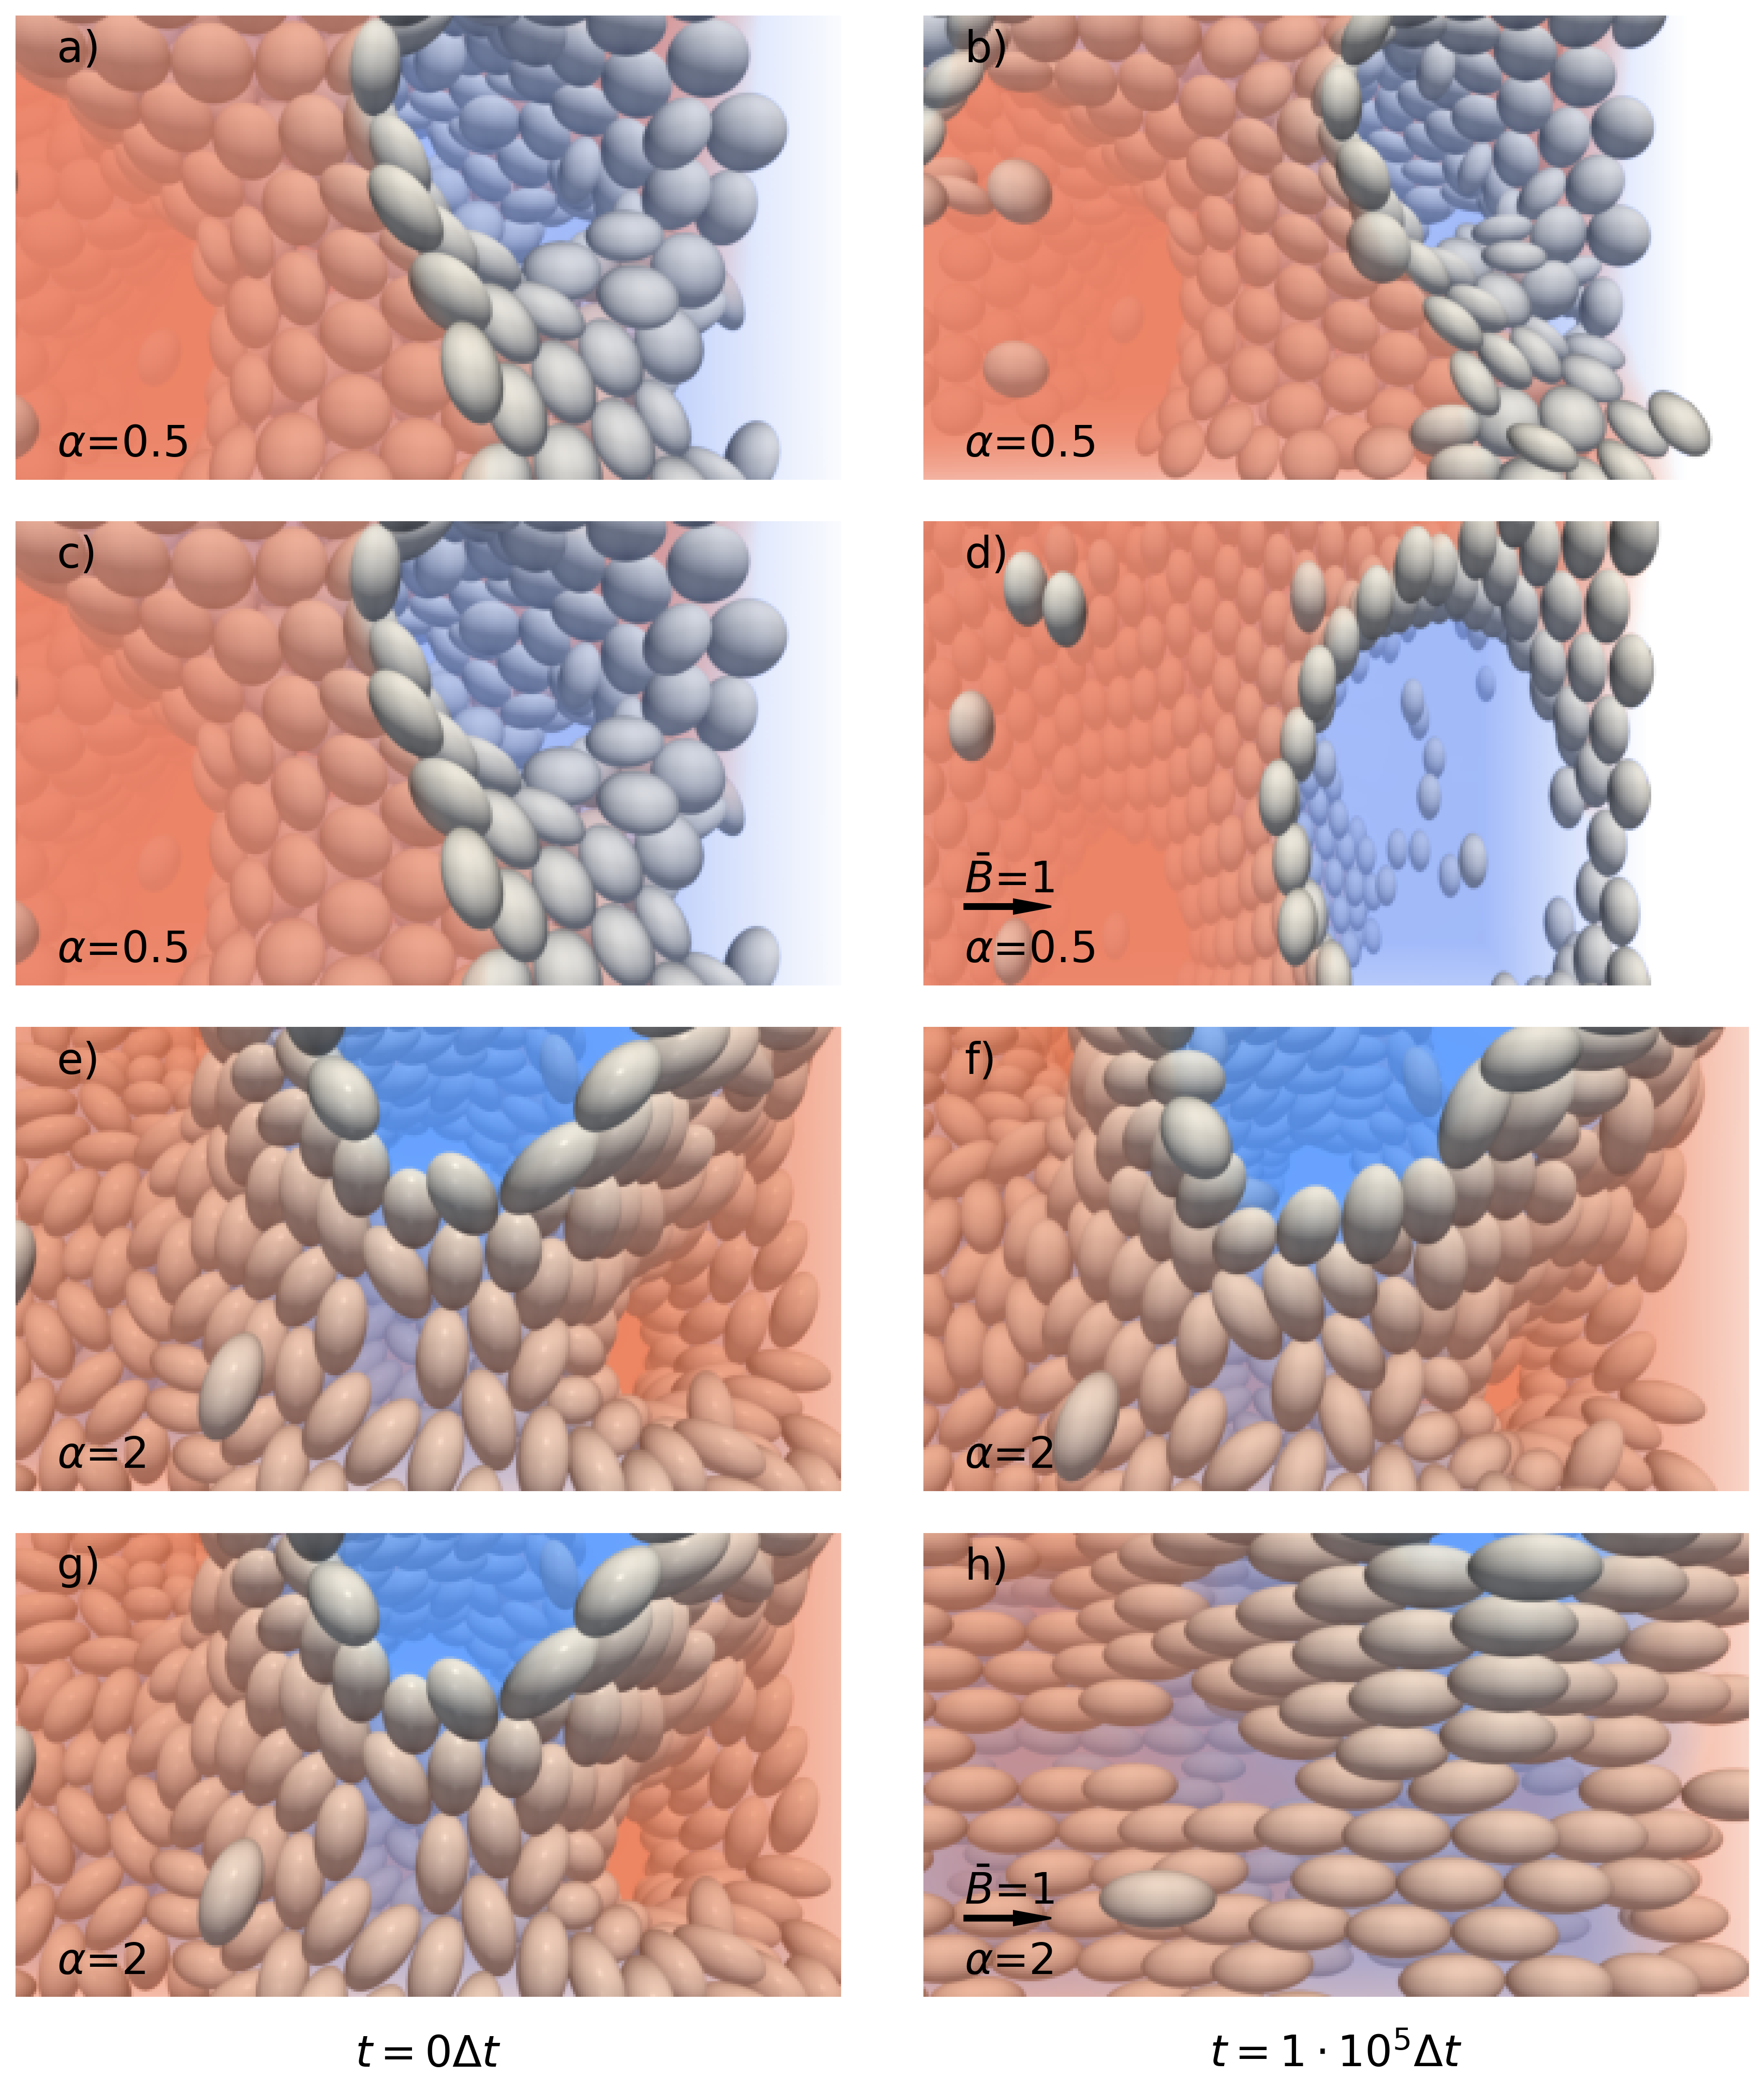
\includegraphics[scale=0.4]{../figures/results/paper2/particle_viz-field_on.png} 
\caption{Visualizations of bijels stabilized by prolate ellipsoidal particles at the initial and final timesteps, 
         both in the absence of a magnetic field (top row) and with a magnetic field applied (\(\bar{B}_z = 1\), bottom row). Particle reorientation to the
         applied field can be observed.} 
\label{fig:particle_viz-field_on} 
\end{figure}

To analyze the reorientation of particles to the magnetic field over time, the nematic order parameter of the particle monolayer is calculated. This is done
in the same technique used for Figure \ref{fig:nematic_time}. 

\begin{figure} 
    \centering 
    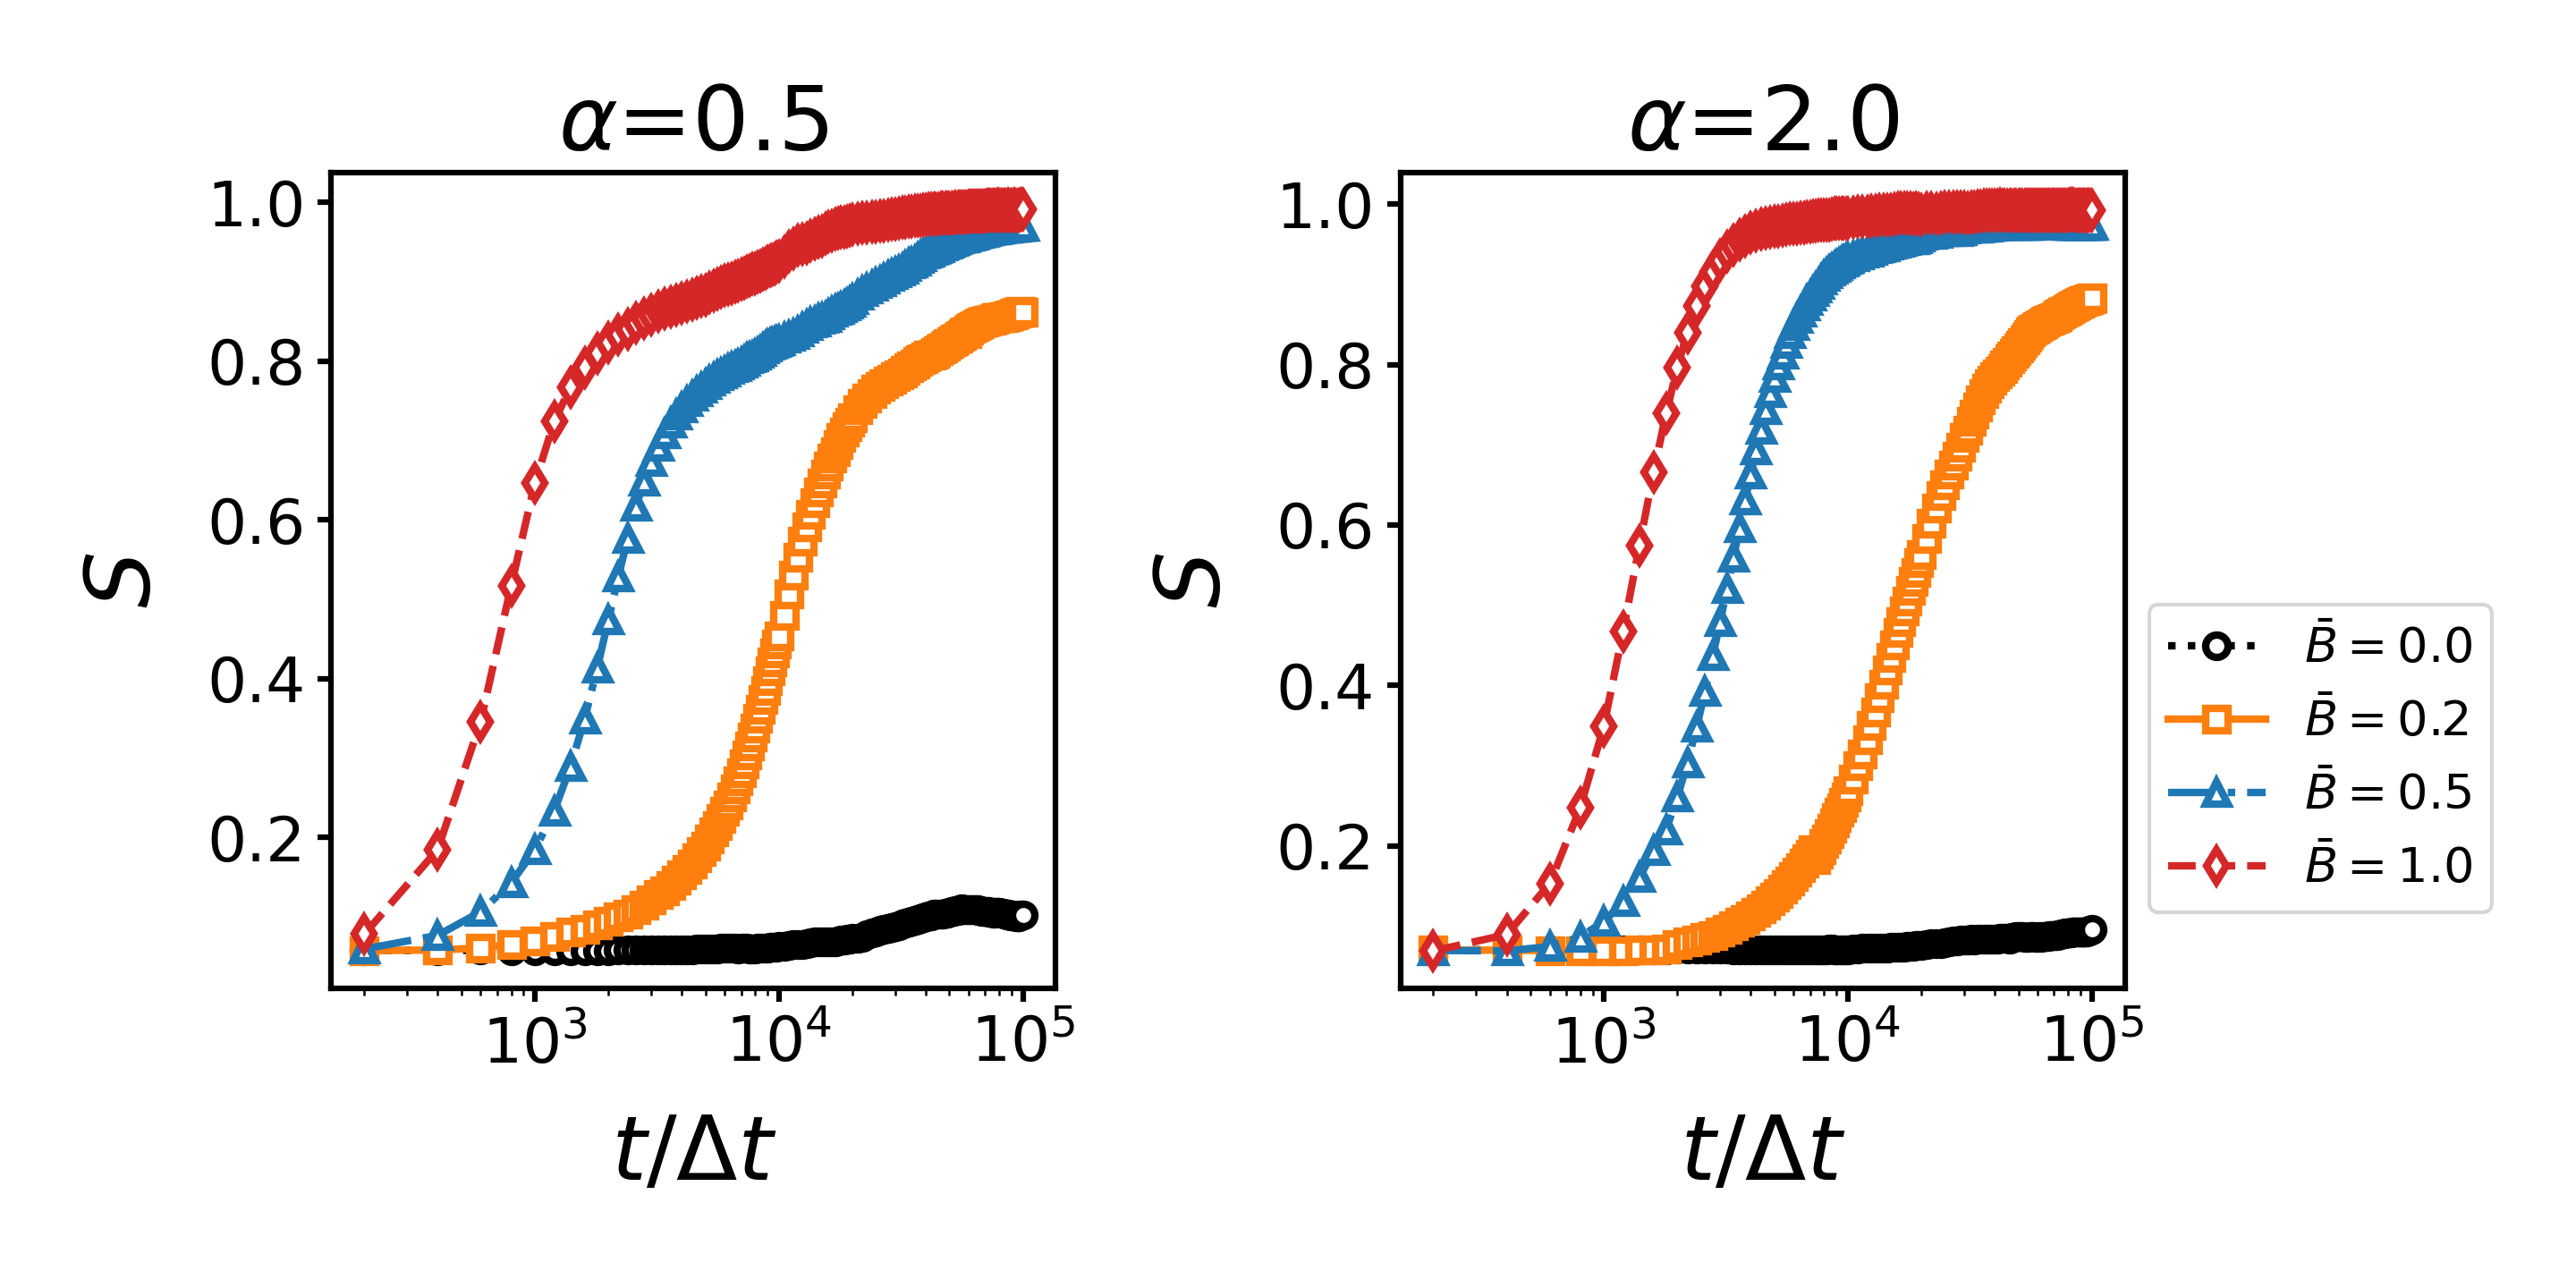
\includegraphics[scale=0.4]{../figures/results/paper2/nematic-field_on.png} 
    \caption{Evolution of the nematic order parameter \( S \) over time for bijels stabilized with disc-like particles (left) and rod-like particles (right), 
             after the application of varying magnetic field strengths.} 
    \label{fig:nematic-field_on} 
\end{figure}

From Figure \ref{fig:nematic-field_on}, as field strength increases, particles exhibit earlier and more pronounced alignment, with \( S \) approaching unity 
for \( \bar{B} = 1.0 \), indicating strong global nematic order. In contrast, systems with no applied field (\( \bar{B} = 0 \)) remain disordered throughout, 
with low \( S \) values. The time-dependent development of nematic ordering reflects the interplay between magnetic torque and interfacial mechanics. 
The increase in \( S \) demonstrates the application of a constant magnetic field causes particle to rotate at the interface to align with the magnetic field.
Linking the alignment of the particles to the domain size change showed in Figure \ref{fig:domain_size-field_on}, the rotation of particles to the magnetic field 
overcomes the initial interfacial jamming. allowing particles to realign to the field. As alignment 
progresses, the particles re-jam. In Chapters 4 and 5, the application of the magnetic field modified the angle of the particle to the interface and the
local packing of the particles. This was caused by orientational of the particles to the magnetic field causing direction dependent cessation of coarsening.
To understand how the rotation of particles affects the particle monolayer, the interfacial angle $\langle \psi \rangle$ is analyzed to understand
how the nematic transition takes place at the interface. $\langle \psi \rangle$ is calculated in the same method as that used to generate Figure \ref{fig:psi_time} 
in Chapter 4, with the results presented in Figure \ref{fig:interface_angle-field_on}. 

% `To understand the interfacial dynamics, the interface angle and the lo This interpretation motivates complementary measurements of the interfacial angle \( \langle \psi \rangle \) and local 
% packing order \( \langle Q_6 \rangle \), which together provide deeper insight into how the transition from disordered to ordered interfacial states is governed by 
% field strength and particle anisotropy.

% The snapshot shows that in the absence of a magnetic field, minor variations in particle orientation and position occur as the bijel is not jammed, as 
% previously observed by Günther et al.~\cite{gunther_timescales_2014}. However, the application of a magnetic field induces clear orientational ordering of the 
% particle monolayer, with particles aligning along the field direction and reorganizing into distinct interfacial arrangements. Newton et al. showed that
% the lowest energy state of arrays of ellipsoidal particles are not at the same orientations to one another when tilted by a magnetic field at an interface.
% \cite{newton_capillary_2018} These changes suggest that both 
% capillary forces and steric hindrance are modified upon field application. While particles naturally prefer to lie flat at the interface to minimize interfacial 
% adsorption energy, the applied field competes with this tendency, reorienting the particles and disrupting their initial packing. The angle of the particle to the
% interface can be used to characterize the reorientation of particles to the magnetic field. The calculation is done in the same way as what is done in Figure
% \ref{fig:psi_time} in Chapter 4.'

\begin{figure} 
    \centering 
    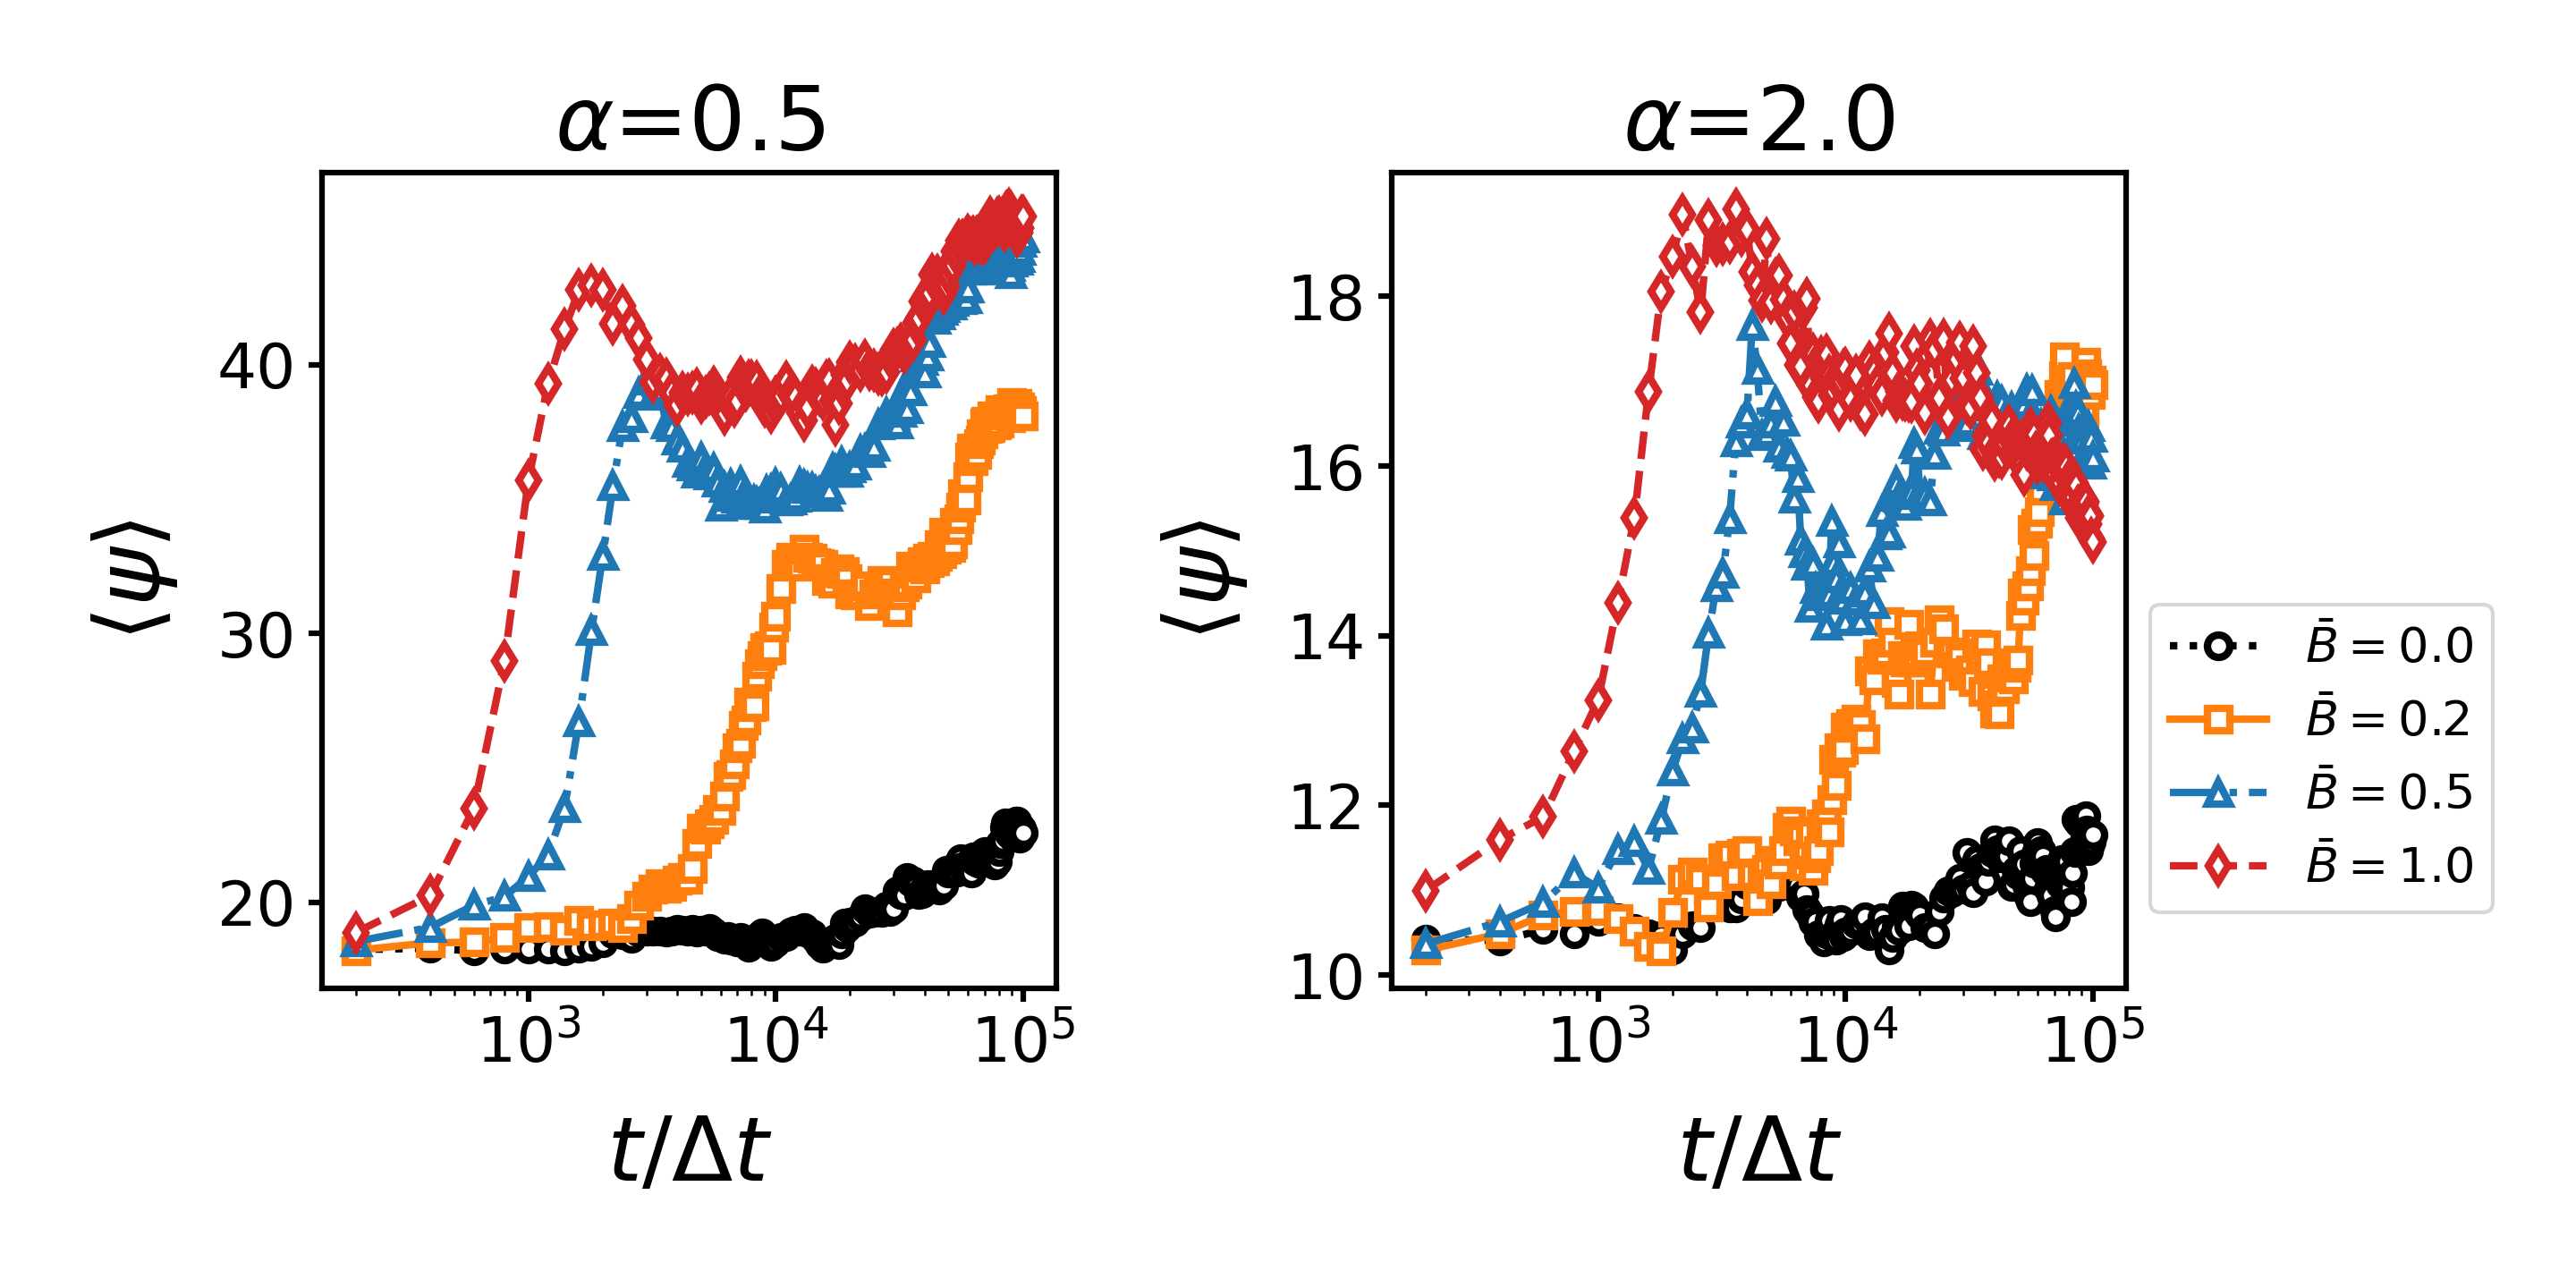
\includegraphics[scale=0.6]{../figures/results/paper2/psi-field_on.png} 
    \caption{Plots of the evolution of the average interface angle \(\langle \psi \rangle\) over time for bijels stabilized 
             by oblate (left) and prolate (right) ellipsoidal particles under varying magnetic field strengths. The response of \(\langle \psi \rangle\) 
             differs notably between the two particle morphologies.} 
    \label{fig:interface_angle-field_on} 
\end{figure}

For bijels stabilized by oblate particles, \(\langle \psi \rangle\) initially increases from approximately \(19^\circ\), indicating that the particles, which begin 
in an approximately flat configuration at the interface, begin to tilt out of the plane in response to the applied field. After a brief decrease or plateau, the angle 
resumes increasing before stabilizing. This behavior suggests that particles first reorient under magnetic torque but are temporarily resisted by interfacial tension 
and capillary constraints. Once the interface begins to deform in response to particle tilt, the system eventually jams in a new configuration, locking the particles 
at an elevated angle. Both the rate of initial tilt and the duration of the plateau phase increase with field strength, and the final value of 
\(\langle \psi \rangle\) is positively correlated with the magnitude of the applied field.

For bijels stabilized by prolate particles, a similar trend is observed. The initial value of \(\langle \psi \rangle\) starts around \(10^\circ\), gradually increases, 
and then exhibits a plateau followed by a slight decline. While the rate and magnitude of the initial increase are field-dependent, the final values converge more 
closely across different field strengths, suggesting that the field sensitivity of interface tilt is weaker for prolate particles. The overall changes in \(\langle \psi \rangle\) 
are also smaller in magnitude compared to those in oblate systems, indicating that prolate particles experience less pronounced reorientation at the interface. This is due to 
the smaller effective lever arm for magnetic torque in prolate particles, which limits their rotational response to the field. 

While the interface angle \(\langle \psi \rangle\) provides insight into the out-of-plane orientation of particles in response to magnetic field application, 
it does not capture how particles reorganize at the interface, observed in Figure \ref{fig:microstructure_viz-field_on} Since the evolution of microstructure is 
influenced not only by tilt but also by the steric effects of interfacial particles, we also assess the Steinhardt bond orientational parameter. The Steinhardt
bond orientational parameter is calculated using the Freud package using the same technique described in Equation \ref{eq:steinhardt_definition}. The results
are plotted in Figure \ref{fig:Q6-field_on}.

\begin{figure} 
    \centering 
    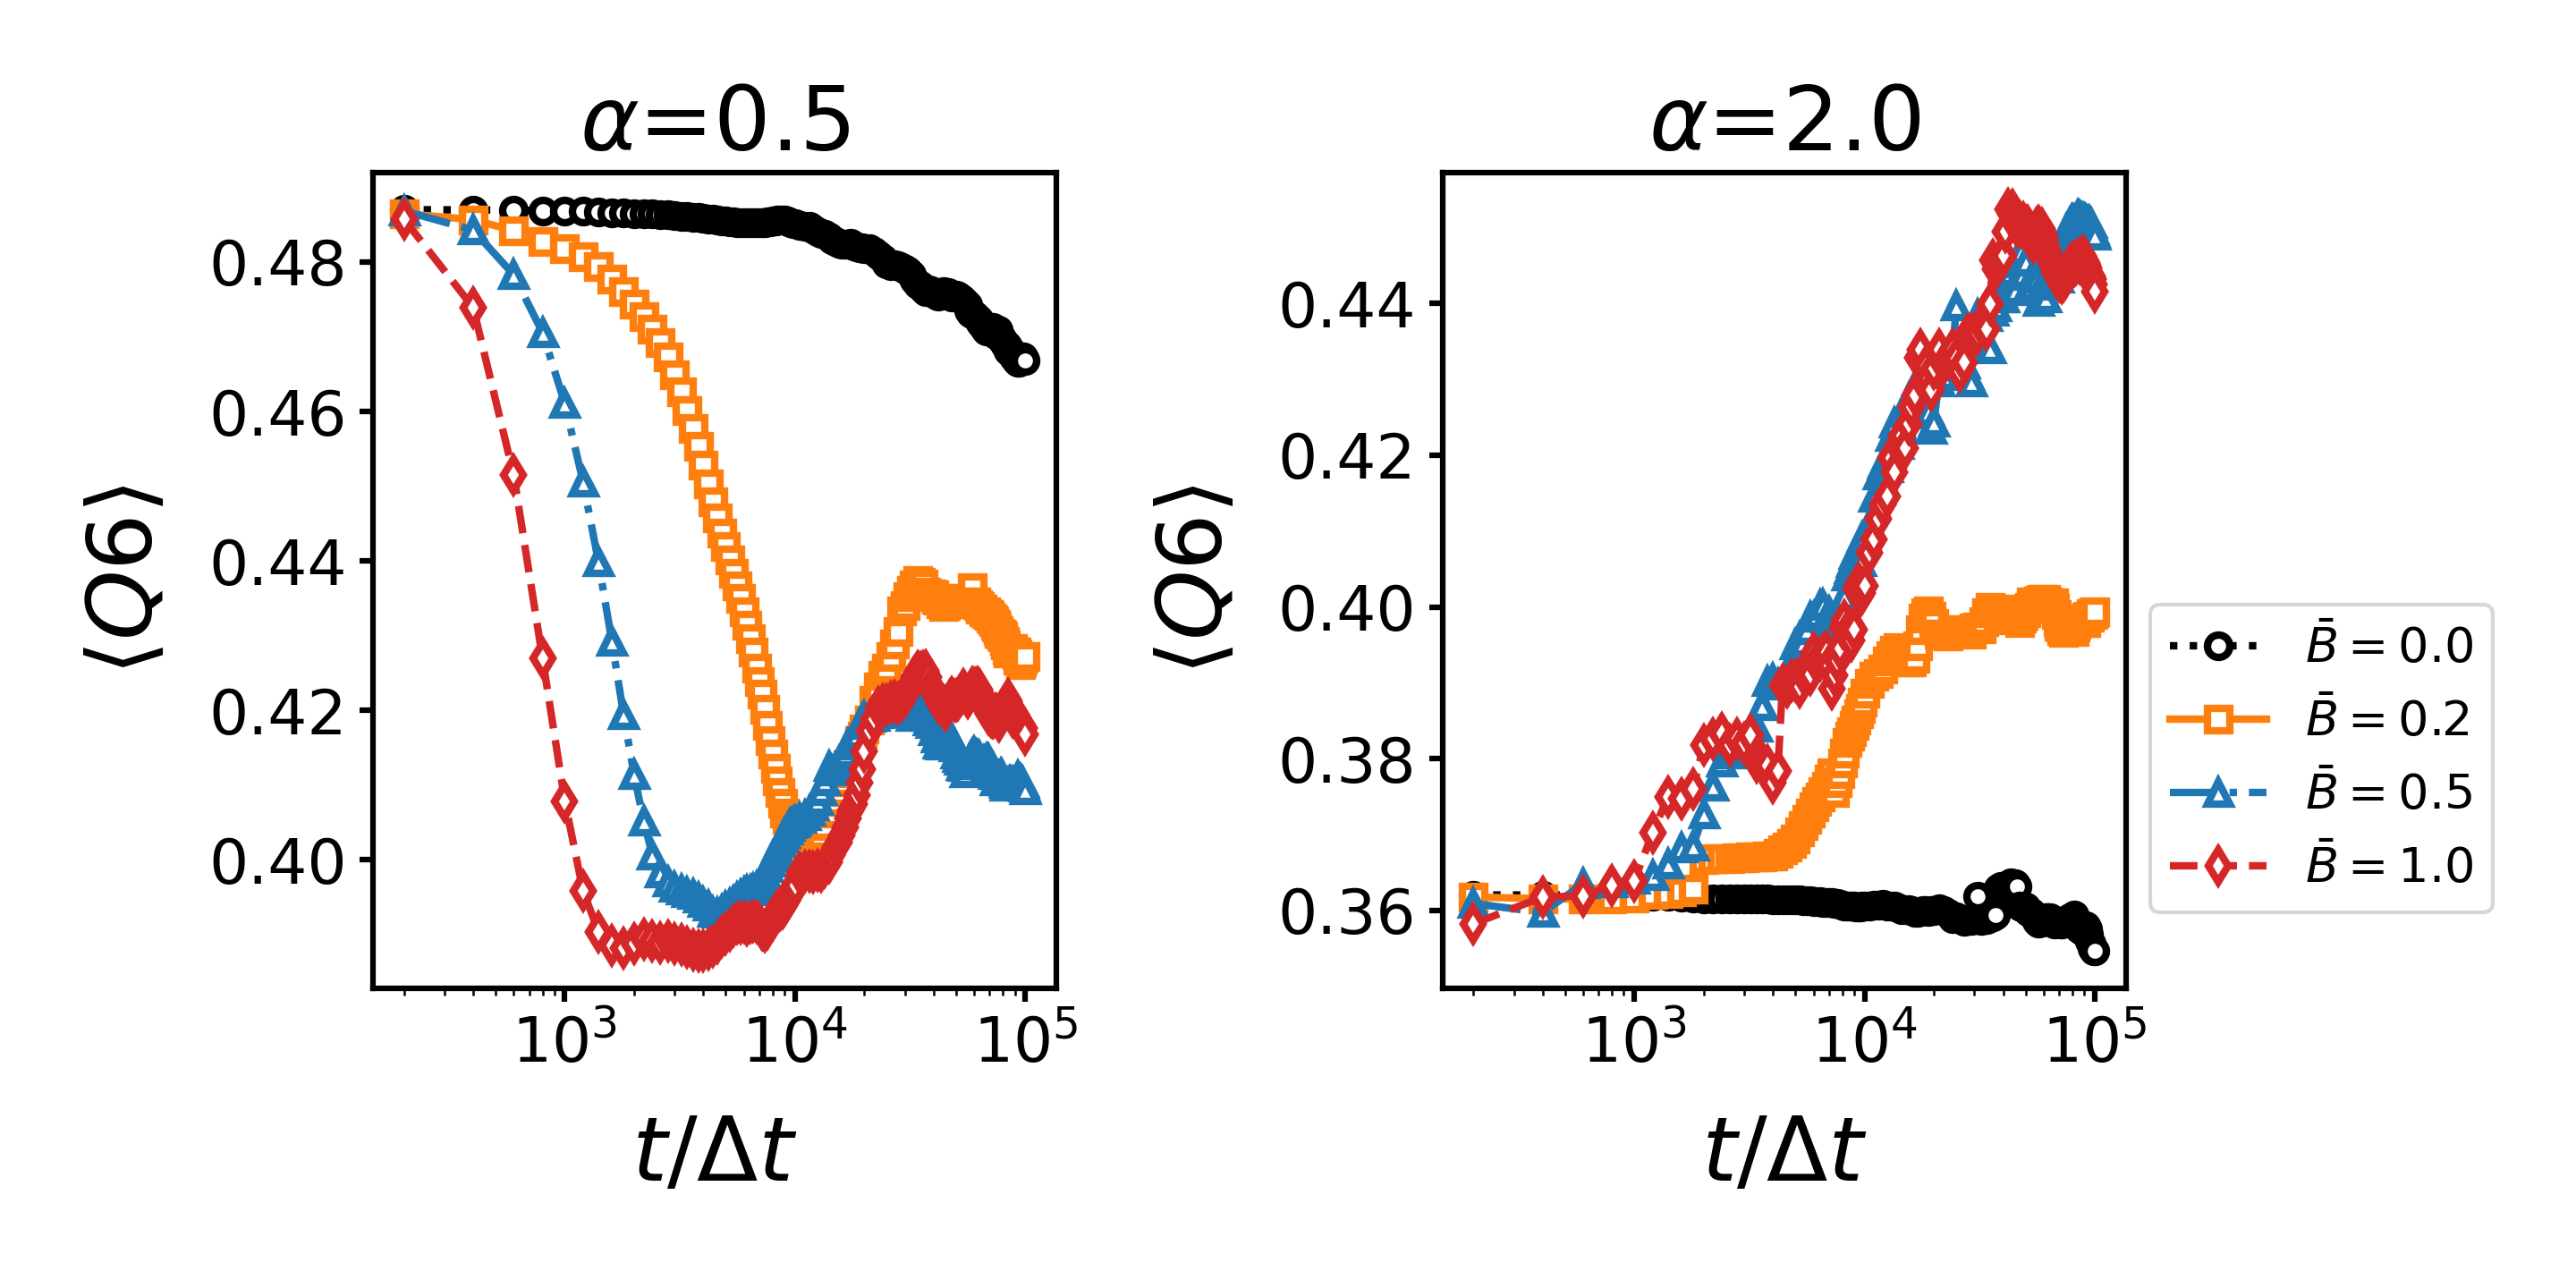
\includegraphics[scale=0.6]{../figures/results/paper2/Q6-field_on.png} 
    \caption{Plots of the time evolution of the six-fold Steinhardt bond order parameter \(\langle Q_6 \rangle\) for bijels 
             stabilized by oblate (left) and prolate (right) ellipsoidal particles under varying magnetic field strengths. The dynamics of interfacial ordering differ 
             significantly between particle morphologies with \(\langle Q_6 \rangle\) decreasing over time for oblate particles and increasing for prolate particles.} 
    \label{fig:Q6-field_on} 
\end{figure}

From Figure \ref{fig:Q6-field_on} the time evolution of \(\langle Q_6 \rangle\) can be qualitatively divided into three regimes;
an initial transition period, a plateau, and a final reordering or jamming phase.
For oblate particles, application of the magnetic field initially causes a sharp decrease in \(\langle Q_6 \rangle\), reflecting a disruption of the 
pre-existing interfacial order as particles begin to tilt and rearrange. This is followed by a plateau, during which ordering is temporarily suppressed 
as particles continue reorienting. Finally, \(\langle Q_6 \rangle\) begins to increase gradually, indicating partial recovery of local order as the system 
evolves toward a new jammed state. The rate of change of \(\langle Q_6 \rangle\) significantly decreases toward the end of the simulation, suggesting the onset 
of kinetic arrest. In contrast, for bijels stabilized by prolate particles, \(\langle Q_6 \rangle\) increases monotonically with time after the field is applied. The degree 
of ordering and the rate of increase both scale positively with magnetic field strength. The early stage is characterized by a modest rise in \(\langle Q_6 \rangle\), 
followed by a more rapid growth and eventual plateau, indicating progressive in-plane reordering of the particle monolayer as alignment along the field direction 
becomes dominant. The timing and extent of these regimes are also field-dependent with stronger fields result in earlier onset of ordering and higher final values 
of \(\langle Q_6 \rangle\).

The final value of \(\langle Q_6 \rangle\) is dependent on the applied magnetic field strength with oblate and prolate particles being affected by the field in
different ways. The trends match that characterized in Chapter 5, with oblate particles having lower hexagonal ordering upon application of a magnetic field
and prolate particles having a greater magnetic field. This was found to be due to oblate particles preferring to stack when magnetic fields are applied while
prolate particles order end to end ot side to side \cite{dabat_mesoscale_2018, eatson_capillary_2023}. This reordering can also explain why oblate particles
tilt out of the interface more than prolate particles.

Thus far, three key particle-scale phenomena have been characterized in response to the application of a magnetic field. The first is
particle alignment to the field direction, where both oblate and prolate ellipsoids reorient their major axes along the magnetic field vector. The second effect is
changes in particle tilt relative to the fluid interface, reflected in variations of the interface angle \(\langle \psi \rangle\), indicating out of interface 
reorientation driven by magnetic torque. Third, reorganization of the local particle monolayer, as captured by the evolution of the Steinhardt bond order parameter 
\(\langle Q_6 \rangle\), which reflects field-dependent disruptions and recoveries in particle ordering at the interface. Together, these processes 
drive the unjamming of the particle monolayer, causing coarsening of the fluid domains before the interface rejams in place with anisotropy dictated by the orientation
of particles to the magnetic field.

\subsection{Switching off an applied field}
\label{decreasing-the-applied-field}

Bijels are kinetically arrested systems whose long-term structural properties are governed by the stability and arrangement 
of the interfacial particle monolayer. Prior studies on responsive emulsions have shown that even after the removal of external 
stimuli, the microstructure often remains unchanged for extended periods due to the interfacial 
jamming of particles \cite{cui_stabilizing_2013}. Similarly, when assessing the kinetic arrest of bijels shown 
in Figure~\ref{fig:hysteresis_curve}, we observed that reducing or removing the magnetic field did not 
lead to a reversal of domain coarsening or particle realignment, suggesting an inherent structural resilience once the bijel 
has stabilized.

Gunther et al. also showed that bijels stabilized by ellipsoidal particles exhibited timescales 
of response distinct from bijels stabilized by spherical particle due to steric effects between ellipsoidal particles.
Therefore, this section will seek to understand to what extent the initial particle order affects the 
bijel's capacity to relax or restructure upon removal of the field. To explore this, 
we now examine the post-stimulus structural response of bijels formed under different field conditions 
\(\bar{B}_{\text{template}} = 0.0, 0.2, 0.5, 1.0\). After allowing each structure to fully stabilize under a 
constant magnetic field, we switch off the field and observe the subsequent time evolution of both the 
microstructure and interfacial particle behavior over a duration of \(t = 10^5 \Delta t\). This analysis aims to 
clarify the mechanisms that underpin the apparent irreversibility captured in the hysteresis response and further 
assess the role of the particles in bijel stability.

\begin{figure} 
\centering 
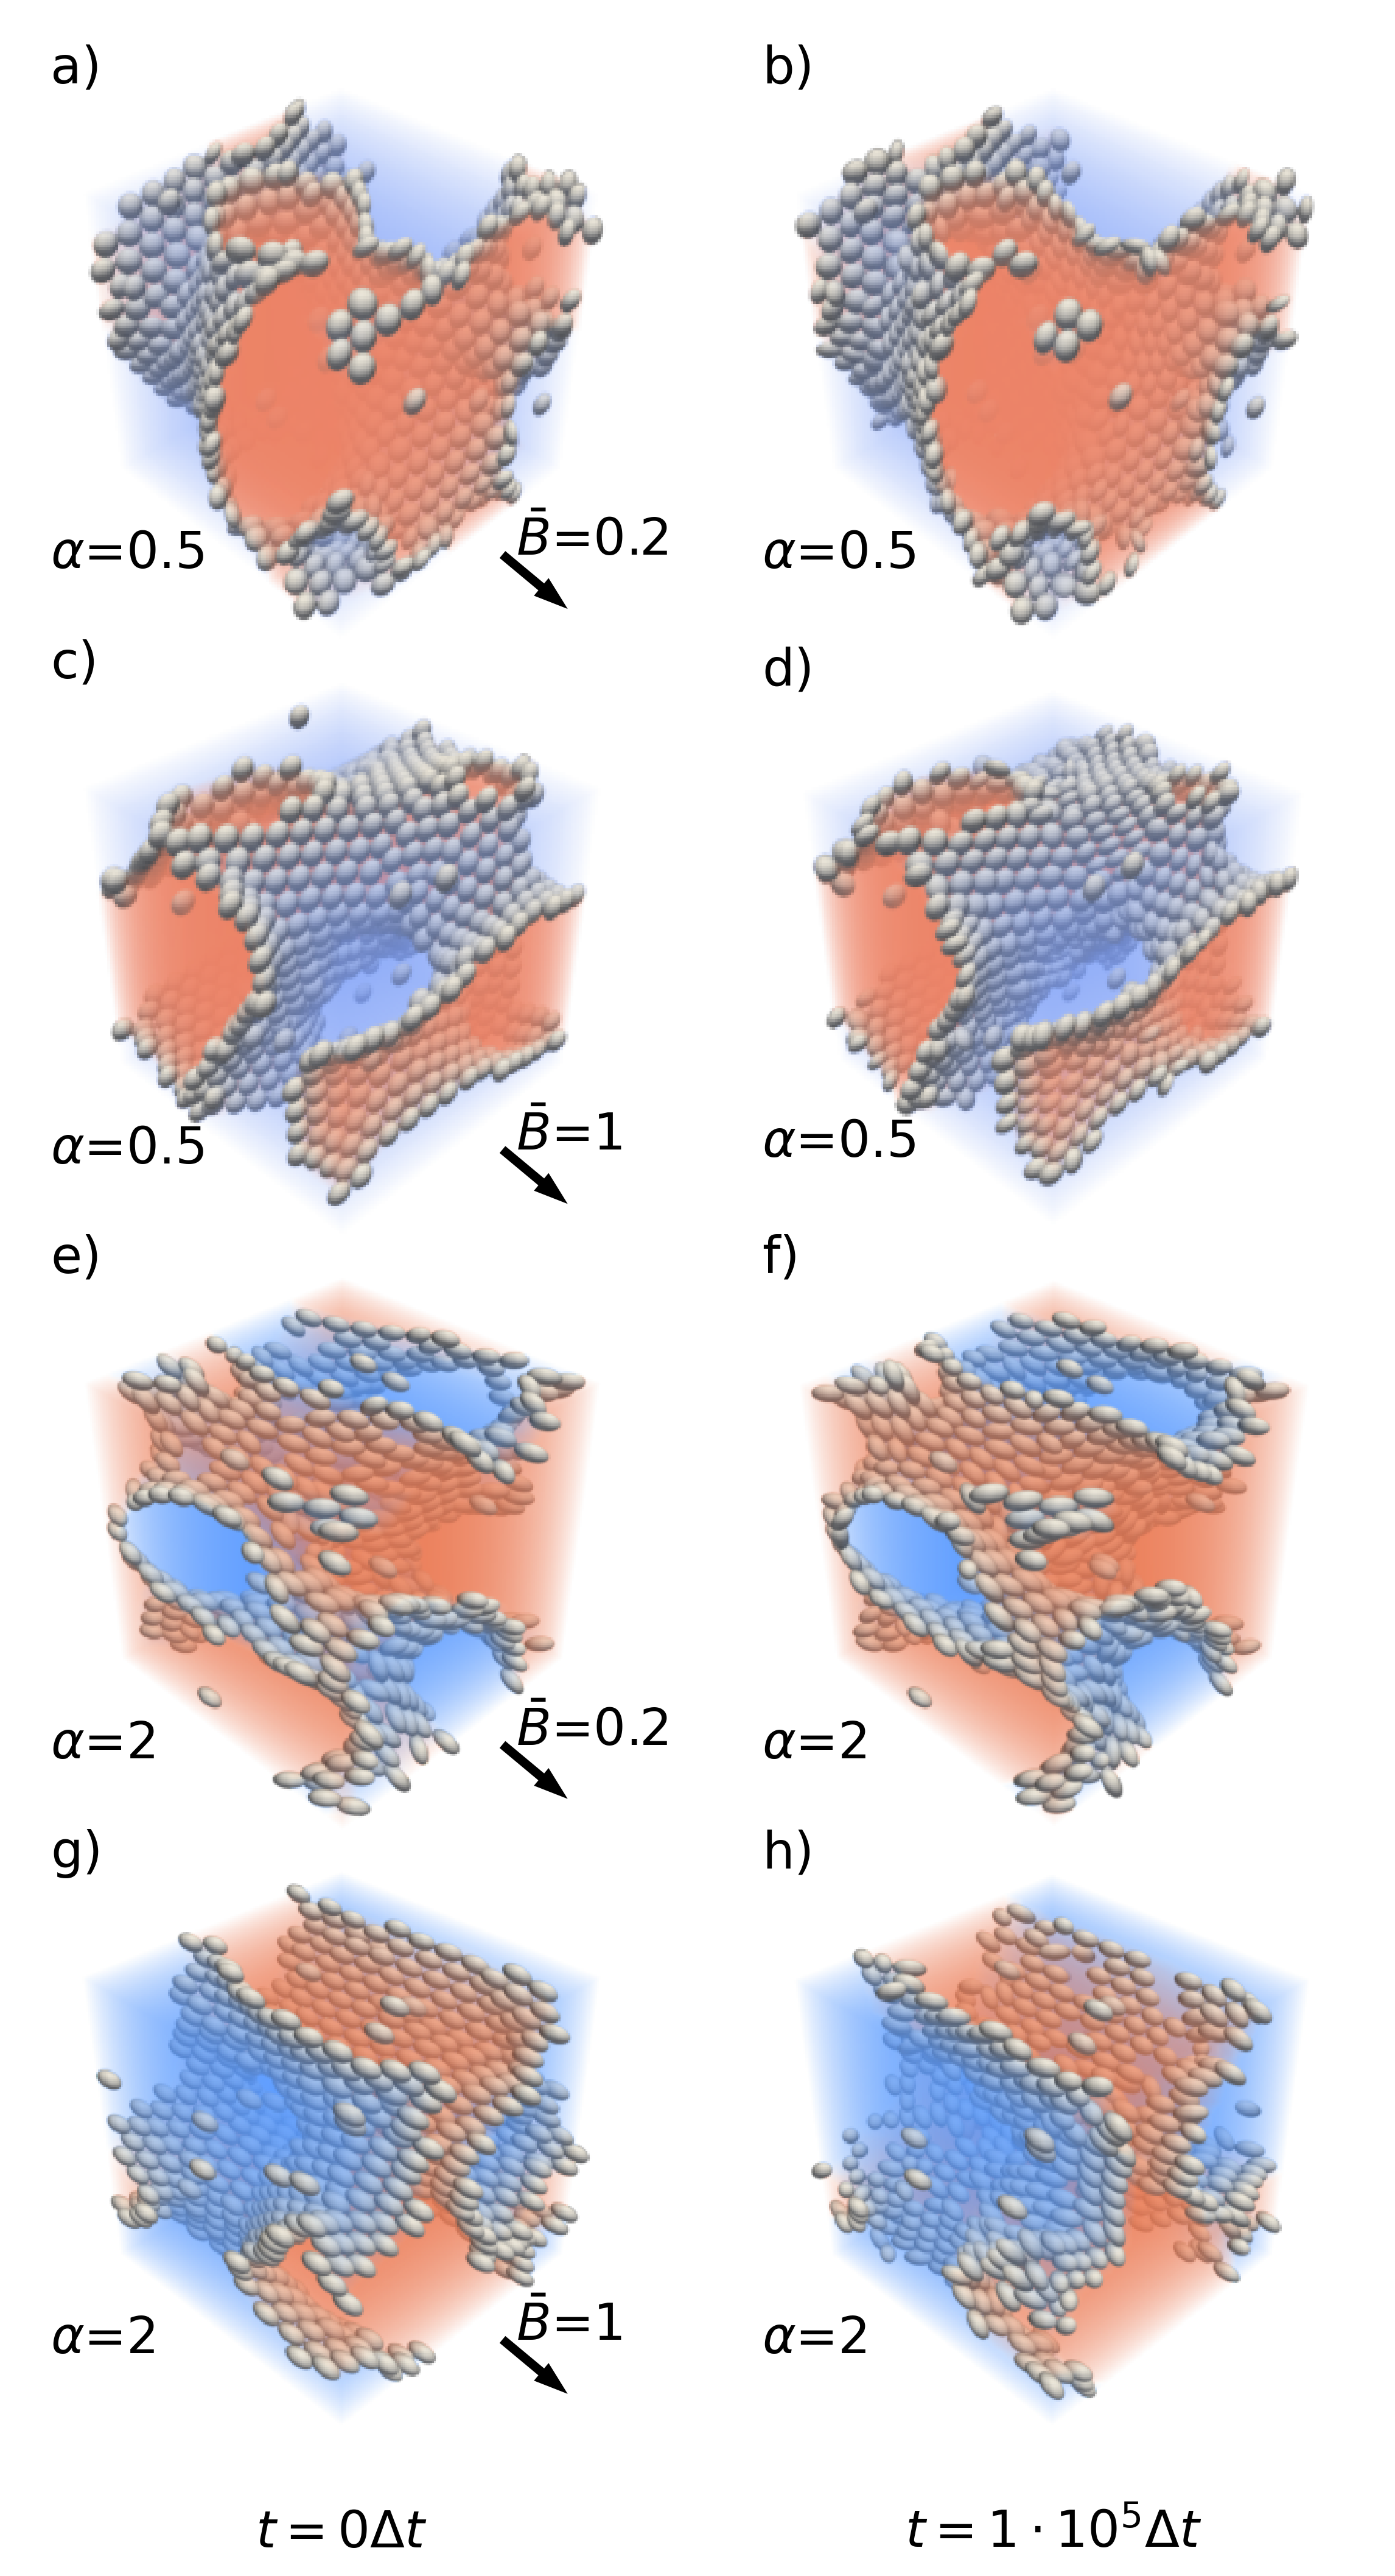
\includegraphics[scale=0.45]{../figures/results/paper2/microstructure_viz-field_down.png} 
\caption{Snapshots of bijels stabilized by prolate ellipsoids at 
         the initial and final time steps after the removal of an applied magnetic field. The top row corresponds to the case where 
         the field is reduced from \(\bar{B} = 0.2 \rightarrow 0.0\), and the bottom row from \(\bar{B} = 1.0 \rightarrow 0.0\)}
\label{fig:microstructure_viz-field_down}
\end{figure}

Figure \ref{fig:microstructure_viz-field_down} shows that in 
both cases, the bulk microstructure remains effectively unchanged over the course of the simulation, highlighting the 
kinetic stability and arrested nature of the bijel.
However, closer inspection of the interfacial particle arrangement reveals that in the
\(\bar{B}: 0.2 \rightarrow 0.0\) case, the particles retain a degree of orientational order, although slight deviations 
from the field-aligned configuration begin to emerge. In contrast, for \(\bar{B}: 1.0 \rightarrow 0.0\), where the 
initial nematic order was stronger, the particles exhibits more apparent disorganization by the final time step. This 
suggests that while the jammed interface resists large-scale rearrangement, there is a gradual relaxation of particle 
orientations in the absence of the aligning field. The extent of this relaxation correlates with the initial field strength when 
the field is removed. We probe the effect of these reorientations by calculating the time evolution of the domain size
in Figure \ref{fig:domain_size-field_down}

\begin{figure} 
\centering 
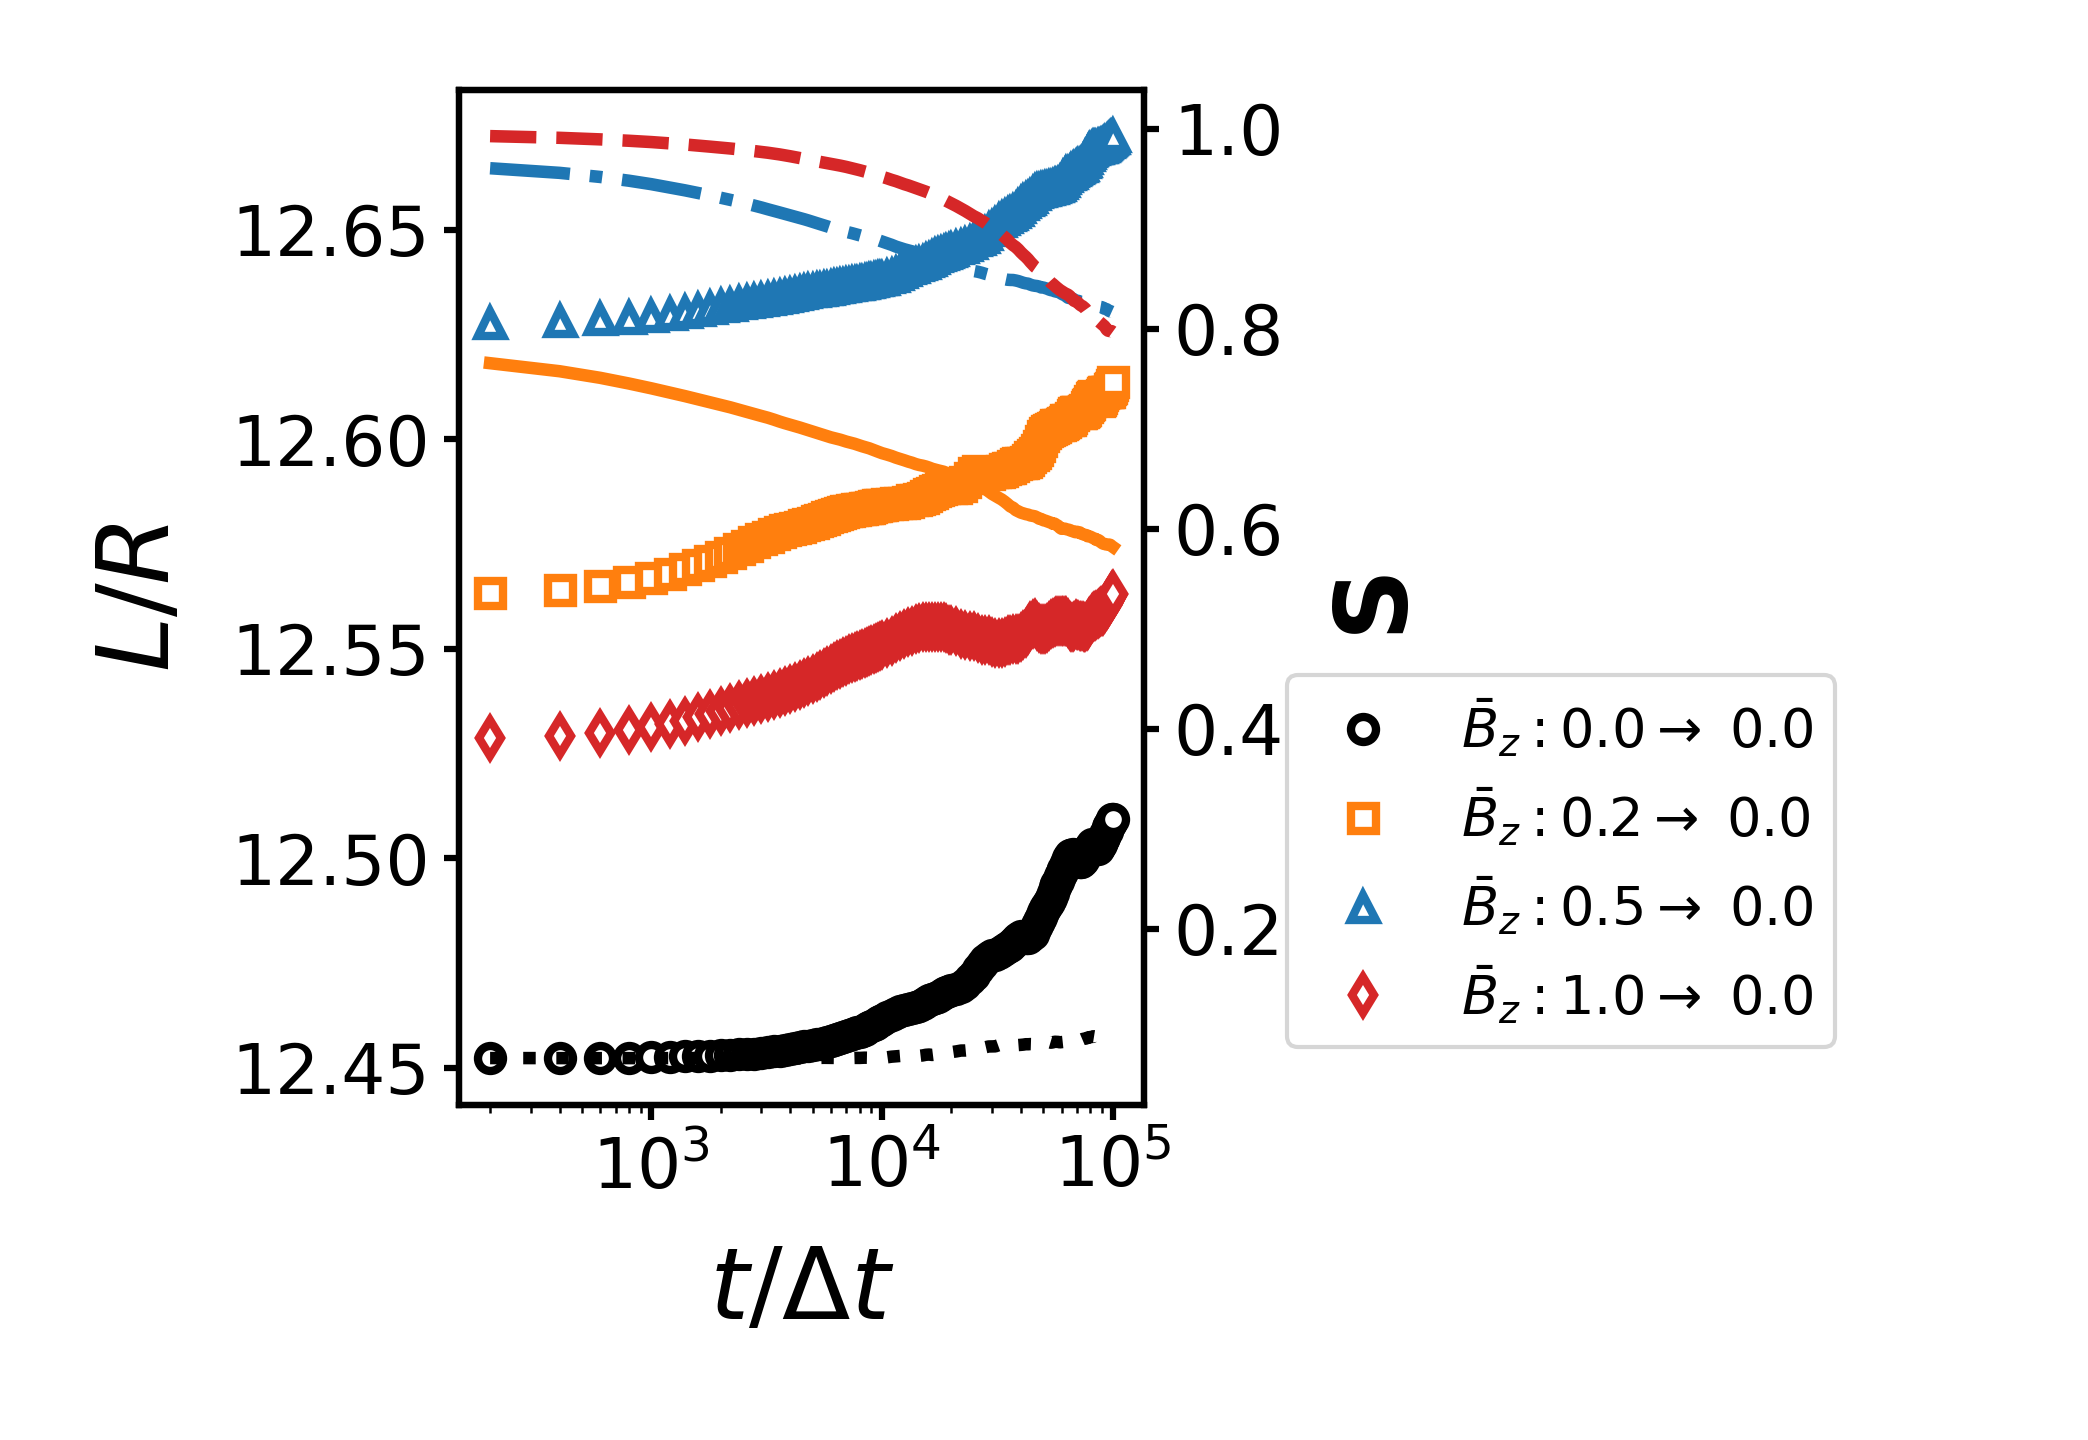
\includegraphics[scale=0.6]{../figures/results/paper2/domain_size-field_down.png} 
\caption{Plot of the spherically averaged domain size normalized with $R_p$ of the particle and the nematic order parameter of each bijel over time. 
         Each color represents bijel templates made with different field strengths $\bar{B}$. We show that there is domain coarsening when the field 
         is switched off, along with a reduction in the ordering of the particles.} 
\label{fig:domain_size-field_down} 
\end{figure}

Figure~\ref{fig:domain_size-field_down} presents the time evolution of the normalized domain size (\(L/R\)) for bijels stabilized by oblate 
(left) and prolate (right) particles following the removal of an applied magnetic field. For all systems except oblate particle stabilized 
bijel with \(\bar{B}: 0.0 \rightarrow 0.0\), a modest degree of domain coarsening is observed. This slow, steady increase in domain size 
indicates that while the global microstructure remains largely intact, minor structural rearrangements may still occur post-stimulus, particularly 
at long timescales. This behavior is more prominent in prolate particle systems, suggesting that elongated particles 
may provide greater local flexibility for slight monolayer relaxation without disrupting the overall network.
A notable exception arises in the oblate \(\bar{B}: 0.0 \rightarrow 0.0\) case, which exhibits a pronounced 
increase in domain size at later times. These results reinforce the interpretation that bijel microstructure 
is resilient to field removal, with no meaningful reversal in the fluid once jamming has occurred even though local particle reorientation occurs.

\section{Conclusion}
% \section[Conclusion]{Conclusion\protect\footnote{Sections of this chapter appear in a manuscript submitted to Springerlink as part of the International Conference on Computational 
% Science (ICCS) 2025 in the Computing and Data Science for Materials Discovery and Design track, submission number 259 and is
% reproduced with permission of Palgrave Springer Nature.}}

In this work, we investigated how magnetic fields influence the structure and dynamics of bijels stabilized by magnetically responsive ellipsoidal particles. Motivated 
by the relevance of bijels in applications such as catalysis, membrane filtration, and drug delivery, we explored how external stimuli can enable in-situ control over 
microstructure in these systems. Using hybrid Lattice Boltzmann-Molecular Dynamics simulations, we characterized the structural response of formed bijels by investigating
the effect of applying a magnetic field and the initial microstructure on the structural response characterized. We first demonstrated that bijels subjected to increasing 
magnetic field strength exhibit kinetic arrest in its structural response, where the domain size increases with field application but does not revert upon field removal.

When investigating the effect of the application of magnetic fields, our results revealed that applying magnetic fields post-formation induces domain coarsening up to 5\%, with 
field-induced anisotropy dependent on particle shape. These changes arise from particle reorientation to the field, followed by 
local unjamming and interfacial rearrangement before re-jamming occurs, as characterized using the average interface angle of the particles and the 
Steinhardt bond orientational order parameter. In contrast, removing the magnetic field had little effect 
on bijel structure. Domain size and anisotropy remained largely unchanged, regardless of initial particle order. While minor relaxation in particle alignment was observed, 
capillary forces alone were insufficient to drive significant structural reorganization.

These results show that rapid coordinated reorientation of the particle stabilizers is necessary to induce structural response in bijels. This is illustrated through structural response
of bijels occurring upon application of the field, causing rapid realignment of particles to the applied field direction while slow realignment of particles away from
the field when switching the field off generated no meaningful changes in the microstructure.

While our simulations offer insights into the tunability of bijels, they were limited to a single set of fluid and particle parameters. Future work could explore the 
effects of particle size, volume fraction, interparticle forces, and field orientation or gradients, all of which may unlock additional control over bijel structure.
Ultimately, this study establishes a foundation for stimuli-responsive bijels, showing how particle-level interactions and monolayer dynamics translate into controllable, 
application-relevant changes in material microstructure.

\chapter{Rheological response of bijels under magnetic fields}

% Previous work into shearing bijels have demonstrated how particles prefer to move in the direction of shear and if strong enough, even detach from the interface. \cite{bonaccorso_shear_2020} It has also been shown how at curved interfaces, ellipsoidal particles  

\section{Introduction}

While the microstructure and synthesis techniques for bijels have been explored in earnest, the rheology of bijels
has remained relatively unexplored. Some interesting phenomena for bijels and shearing include the 
presence of monogels, made by remixing the phase separated liquid domains of the bijel while the electrostatic
interactions between particles maintains the structure of the particle monolayer. \cite{sanz_colloidal_2009} 
Monogel formation has been observed in lutidine/water and styrene/butadiene oligomer based bijels but not ethane-diol nitromethane based bijels
\cite{sanz_colloidal_2009, bai_dynamics_2015, tavacoli_novel_2011} Computational Investigations have identified that confined bijels under shear undergo elongation of
the domains in the direction of shear succeeded by particle detachment from the interface and eventual failure of the bijel. \cite{bonaccorso_shear_2020}
More recently, bijels have been identified to be 2D glasses percolating in 3D space, characterized through comparing the complex rheology of bijels against
colloidal gels made from silica particles with electrostatic interactions. \cite{ching_bijel_2022} 

In many of the manufacturing techniques outlined the rheological properties are essential in ensuring that 
the casting mixture remains processable. \cite{haase_continuous_2015,haase_situ_2016} In STrIPS, the flow rate of the casting mixture and the co-solvent
control the microstructure of the bijel and the morphology of the resulting bijel material, controlling whether droplets or ropes are synthesized. \cite{haase_continuous_2015}
When investigating the effect of magnetic fields on the rheological properties of suspensions, it has been shown that the viscosity of ferrofluids increases substantially due
to the self assembly of particles restricting the flow of fluid, greatly increasing the viscosity of the ferrofluid. cite{qiao_magnetorheological_2012} The application
of shear onto suspensions can also cause shear banding as interparticle interactions mediate particle fluid interactions, creating localized velocity differences to the bulk.
\cite{xu_relation_2013} Looking into emulsions, the application of magnetic fields increases the viscosity of emulsions, making them more shear thinning than when no field 
is applied.

In past chapters, I identified the microstructure and particle arrangement of bijels stabilized by ellipsoidal particles under magnetic fields and demonstrated
particles morphology specific ordering to the applied magnetic field. I also show that the local ordering of the particles is affected from the application of
the magnetic field. In this chapter, I probe the dynamics of bijels under constant shear to understand how these microstructural and particle monolayer changes
affect the rheology of bijels stabilized by ellipsoidal particles under magnetic fields. First, I define a shear capillary number 
$Ca_s = \frac{\eta_{f} \dot{\gamma} R_s}{\sigma}$ where $\dot{\gamma} = \frac{2u_{LE}}{L_x}$ is the
strain rate and $R_s$ is the size of equivalent spherical particle. \cite{frijters_effects_2012, yang_capillary_2022} In the literature, $Ca_s$ has been between between 0.04 
and 0.16. However, the box size in these simulations were smaller, meaning that these capillary number ranges would exceed the 
maximum mach number the model allows if this same range were used $(Ma \leq 0.03)$. To accommodate this limitation the 
largest capillary number used will be $Ca_s = 10^-4$ which correspond to a maximum of $Ma \approx 0.02$. As all particles used 
have only hard-sphere type interactions, it is expected that the behaviour seen should mimic 2D colloidal glasses 
percolating in 3D space, akin to what Ching and Mohraz saw, with an additional dependence on the direction of shear. 
This would predict the discovery of particle monolayer dependent elasticity and yield stress along with shear thinning 
behavior of the bijels.

To verify these predictions, bijel microstructure will be defined using four processing histories; The first is of a 
bijel simulated under a $\Bar{B} = 1$ magnetic field strength, the second is a bijel stimulated under no field, 
followed by the application of a $\Bar{B} = 1$ field after jamming, the third is a bijel simulated under no field, 
while the final microstructure is a bijel simulated under $\Bar{B} = 1$ magnetic field, followed by switching the 
field off after jamming. This gives insight into the impact of processing history on the shear properties of a bijel, 
in addition to the microstructural and colloidal insights gained. Based on the results in Bonaccorso et al., there 
should be shear driven and shear rate dependent elongation of the domains in the direction parallel to the applied 
shear which in this system will be seen as a reduction in $L_{\perp}$ and an increase in $L_{\parallel}$. 
\cite{bonaccorso_shear_2020} The microstructure anisotropy will also be a factor in the viscosity results, as 
larger domains are more permeable than smaller ones, meaning that bijels where $L_{\perp} > L_{\parallel}$ should 
see less of the domain elongation effects shown in Bonaccorso et al. as the permeability of the bijels rises with 
larger domain size. \cite{bonaccorso_shear_2020}

It is also expected that the effective viscosity will be different between the four microstructures dependent upon the 
degree of nematic ordering and microstructural anisotropy of the bijel. Nematic ordering of the particles in the direction of shear
should resulting in a lowered effective viscosity compared to bijels without nematically 
ordered particles. \cite{xu_relation_2013, vermant_flow-induced_2005} Tracking of the proportion of particles on the 
interface will also yield insight into how the packing of the particles affects the rate at which particles will get 
ejected from the interface. Bonnacorso et al. identified that shear applied onto bijels caused particles to align to the direction of
shear before being ejected from the interface. Systems with a larger $\eta_{eff}$ are predicted to have the largest domains, largest 
difference between initial and final particle order and lowest number of particles left on the interface once steady 
state has been established. 

\section{Results}\label{sec:results_p3}

I begin this investigation by analyzing the rheological response of bijels stabilized by ellipsoidal particles under constant shear.
Specifically, I investigate the effect that particle order has on the rheological response characterized. I am also interested in
identifying the impact that the application of magnetic fields have on the rheological response of the bijel. 
Bijel templates simulated in Aim 1 with no field and a field strength of $\bar{B} = 1$ stabilized with a prolate and oblate particles with a 
particle volume fraction $\phi_p = 0.15$ were used as the starting point for these simulations. Next, I apply a field strength of
$\bar{B} = 1$ or switch off the applied field to all structures. This results in four processing setups; $\bar{B}:0\rightarrow 0$, $\bar{B}:0\rightarrow 1$,
$\bar{B}:1\rightarrow 0$ and $\bar{B}:1\rightarrow 1$. I then define a shear capillary number,  $Ca_s = \frac{\dot{\gamma} R_{s} \eta_{f}}{\sigma}$ where 
$\dot{\gamma}$ is the applied strain rate, $R_s$ is the equivalent spherical radius of the particles, $R_s = 7.9$, $\eta_f$ is the dynamic viscosity of the 
fluid and $\sigma$ is the surface tension of the interface. I use five shear numbers, $Ca_s = 1\cdot10^{-4}, 5\cdot10^{-5}, 1\cdot10^{-5}, 5\cdot10^{-6}, 1\cdot10^{-6}$.

\subsection{Viscosity measurement}

The ordering of the particles play an important role in determining the rheology of suspensions as ordered particles can slip over one another
before the structure breaks. The adsorption of particles on the interface of a bijel could affect how this slip occurs. Previous work investigating
the rheology of bijels have determined shear thinning behavior characterized with a Herschel-Buckley fit equation. \cite{macmillan_rheological_2019} 
I perform this analysis on the structures I have simulated. First, I plot the shear stress over time.

\begin{figure} 
    \centering 
    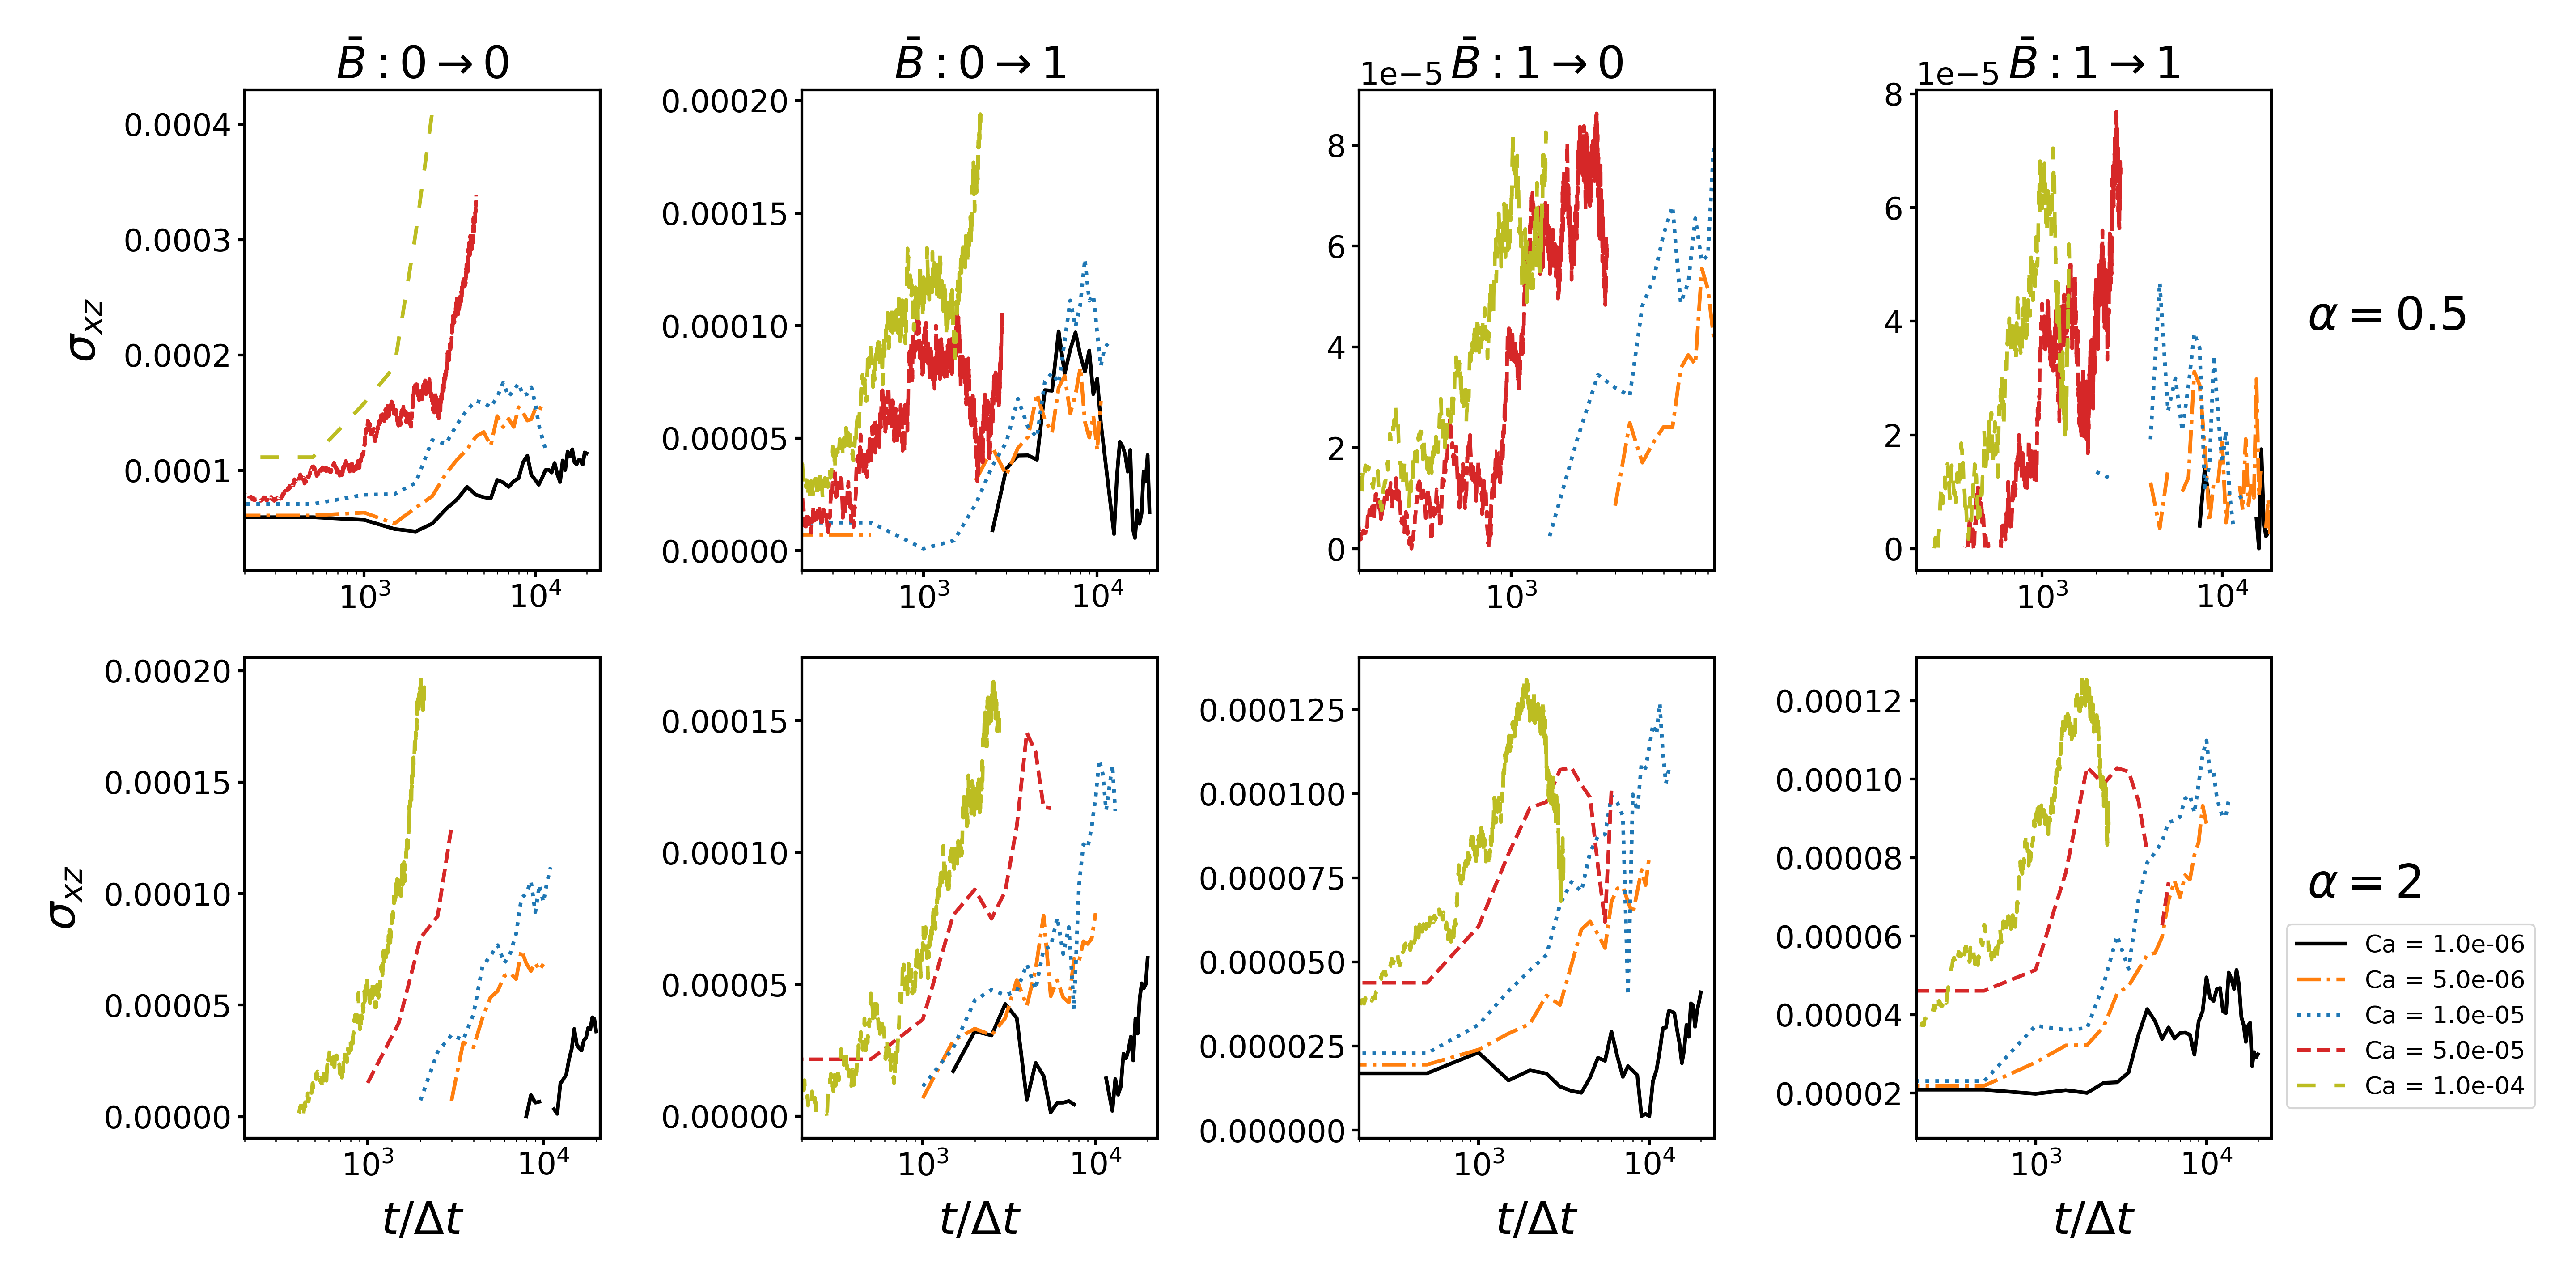
\includegraphics[scale=0.3]{../figures/results/paper3/stress-time_compare.png} 
    \caption{Time evolution of the shear stress of bijels stabilized with ellipsoidal particles as a function of the applied strain rate as
             a function of the initial microstructure and applied magnetic field. The observed stress response is difficult to say when a steady
             state is reached.} 
    \label{fig:stress_time} 
\end{figure}

Figure \ref{fig:stress_time} shows that there is no definitive steady state value of the shear stress obtained in the simulations performed. This is
attributed to the coarsening of the domains and reorientation of particles at the interface. \cite{tavacoli_novel_2011,macmillan_rheological_2019} 
Tavacoli et al. investigated the rheological response of Ethanediol/Nitromethane bijels and identified that upon placement of a needle to calculate the yield
stress of the bijel, the structure of the material was irreversibly altered. \cite{tavacoli_novel_2011} Macmillian et al. identified that repeated 
shearing of a bijel synthesized using direct mixing resulted in degraded mechanical performance. \cite{macmillan_rheological_2019}
To characterize the viscosity, I identify pseudo-steady state regions within each of the shear stress plots and fit the stress identified within this 
pseudo-steady state region to the strain rate. Pseudo-steady state regions are identified by measuring where the rate of change of shear stress is 
smallest for the longest duration. I fit the calculated stress to the applied strain rate using a Herschel-Buckley rheology model defined as
$\sigma_{xz} = \sigma_{y} + K(\dot{\gamma})^{n}$. $\sigma_{xz}$ is the shear stress calculated from the simulation, $\sigma_{y}$ is the yield stress of the bijel, 
$K$ is the flow consistency index and $n$ is the flow index.Where appropriate, I include results corresponding to a shear capillary number of 
$Ca_s = 10^{-6}$ as in many stress responses, $Ca_s = 10^{-6}$ may not always yield usable results. 

\begin{figure} 
    \centering 
    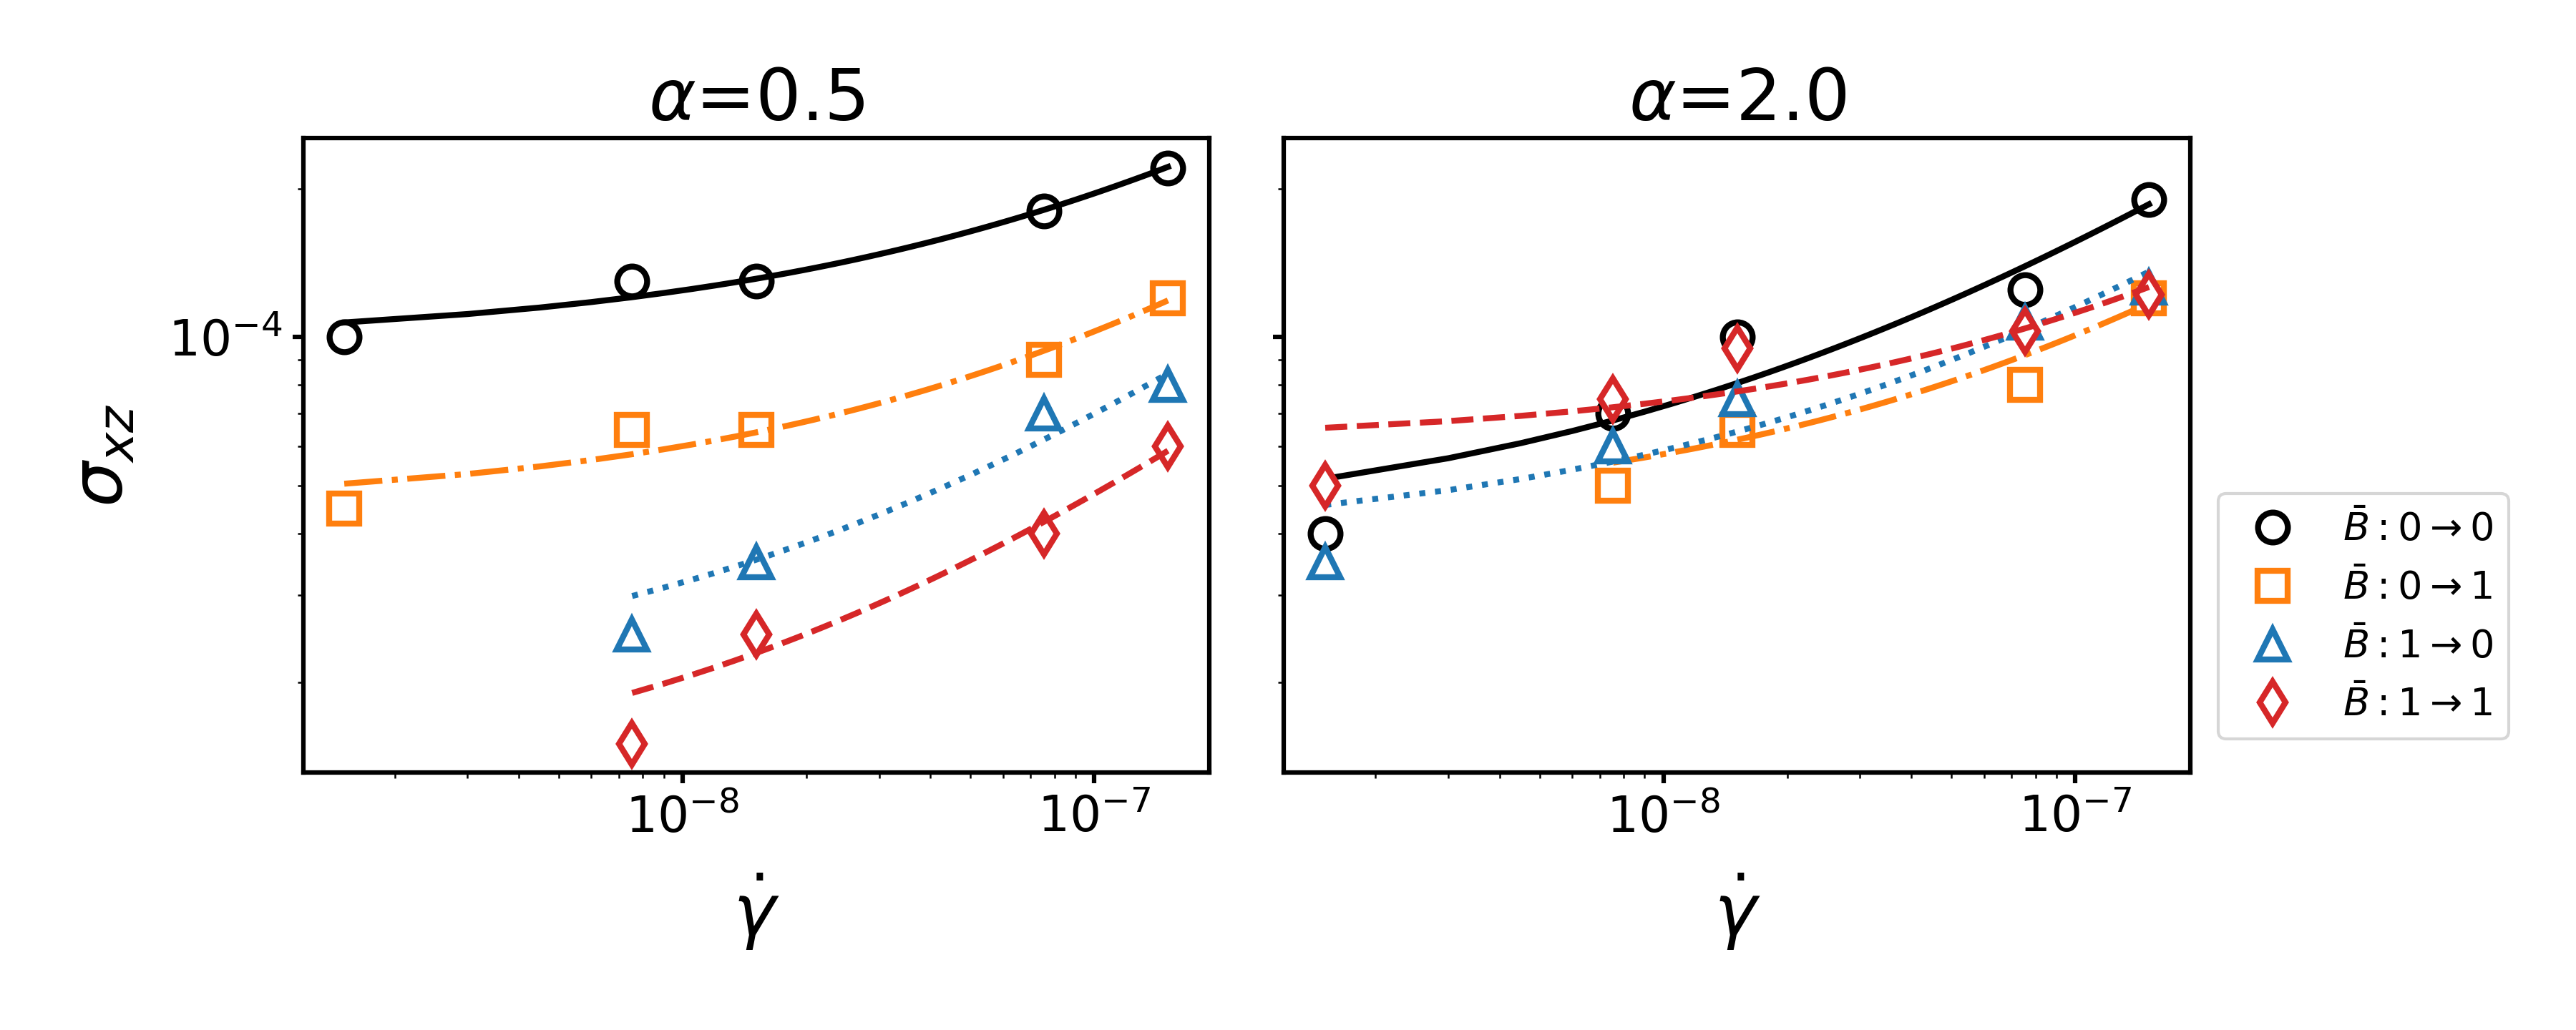
\includegraphics[scale=0.4]{../figures/results/paper3/stress_strain-all.png} 
    \caption{Fitting the experimental shear stress to the strain rate using the Herschel Buckley model. I characterize the bijels are 
             shear thinning in all cases. I show that the bijels become less shear thinning as the particle order increases. I also
             demonstrate that the particle ordering affects the yield stress differently for particles stabilized by oblate and 
             prolate particles.} 
    \label{fig:stress_strain} 
\end{figure}

From Figure \ref{fig:stress_strain}, the slopes of the curve indicate a non-linear shear response to the applied strain rate, suggesting that the rheological properties
are non-Newtonian. Bijels stabilized by prolate and oblate particles also have different shear properties. For bijels stabilized by oblate particles, the stress curves
are more spread out suggesting that there is a larger variance in the properties arising from the change in the initial microstructure of the bijel. From the plot
we can see that the increase in particle order reduces the yield stress of the bijel. For bijels stabilized by rod like particles, the stress response of each processing 
condition is closer together, indicating a smaller variation in the response to the applied magnetic field compared to oblate particles. The shear response upon application
of the magnetic field also suggest that increased ordering of prolate particles makes the bijel more resistant to shear. I quantify the Herschel-Buckley fit parameters and 
tabulate the results in Table \ref{table:rheology_fit}.

\begin{table}[h!]
    \centering
    \begin{tabular}{||c c c c c||} 
     \hline
     Processing & $\alpha$ & $n$ & $K \frac{\Delta m (\Delta t)^{n-2}}{\Delta x} $ & $\sigma_{y} \frac{\Delta m}{\Delta x (\Delta t)^2}$ \\ [0.5ex] 
     \hline\hline
     $\bar{B}: 0 \rightarrow 0$ & 0.5 & 0.511 & 0.999 & $7.168 \cdot 10^{-5}$ \\ 
     \hline
     $\bar{B}: 0 \rightarrow 1$ & 0.5 & 0.579 & 0.944 & $4.008 \cdot 10^{-5}$ \\
     \hline
     $\bar{B}: 1 \rightarrow 0$ & 0.5 & 0.642 & 0.888 & $4.945 \cdot 10^{-5}$ \\
     \hline
     $\bar{B}: 1 \rightarrow 1$ & 0.5 & 0.637 & 0.914 & $1.715 \cdot 10^{-5}$ \\
     \hline
     $\bar{B}: 0 \rightarrow 0$ & 2 & 0.561 & 0.965 & $4.618 \cdot 10^{-5}$ \\
     \hline
     $\bar{B}: 0 \rightarrow 1$ & 2 & 0.609 & 0.944 & $4.101 \cdot 10^{-5}$ \\
     \hline
     $\bar{B}: 1 \rightarrow 0$ & 2 & 0.597 & 0.899 & $5.025 \cdot 10^{-5}$ \\
     \hline
     $\bar{B}: 1 \rightarrow 1$ & 2 & 0.606 & 0.885 & $6.435 \cdot 10^{-5}$ \\ [1ex] 
     \hline
    \end{tabular}
    \caption{Hershel Buckley fit parameters for different processing conditions applied to bijels stabilized by ellipsoidal particles.}
    \label{table:rheology_fit}
\end{table}
 
The results in Table \ref{table:rheology_fit} show that bijels remain shear thinning regardless of the processing history and particle morphology.
The particle morphology dependent differences in the shear response characterized in Figure \ref{fig:stress_strain} are quantified in Table \ref{table:rheology_fit}
where the yield stress differences predicted is clear to see. I also show that bijel templates with an applied field of $\bar{B} = 1$ have larger flow indices \
than bijel templates made with no applied field. The same trend exists here where the application of a magnetic field makes the bijel more Newtonian. I also 
characterize that the yield stress of bijels stabilized with oblate particles decrease as the initial order of the particles and the applied field onto the bijel increase. 
The yield stress of bijels stabilized by prolate particles increases as the initial order of the particles and the applied field onto the bijel increase. In previous aims, I 
characterized that application of magnetic fields created orientational ordering of the bijels and that the local ordering of the bijels change. I 
showed that as magnetic fields were applied, oblate particles have lower local ordering on the interface while for prolate particles it increases.
Past investigations have identified that particle monolayers buckle more easily as local particle ordering decreases. \cite{prakash_buckling_2024} 
They identified that local ordering can enhance stress distribution among particles, making locally ordered particle monolayers better at withstanding shear.
I visualize the ordering of the particles at the interface to the z direction for both particle morphologies at $Ca_s = 10^{-6}$ for the 
case $\bar{B}: 1 \rightarrow 0$.

\begin{figure} 
    \centering 
    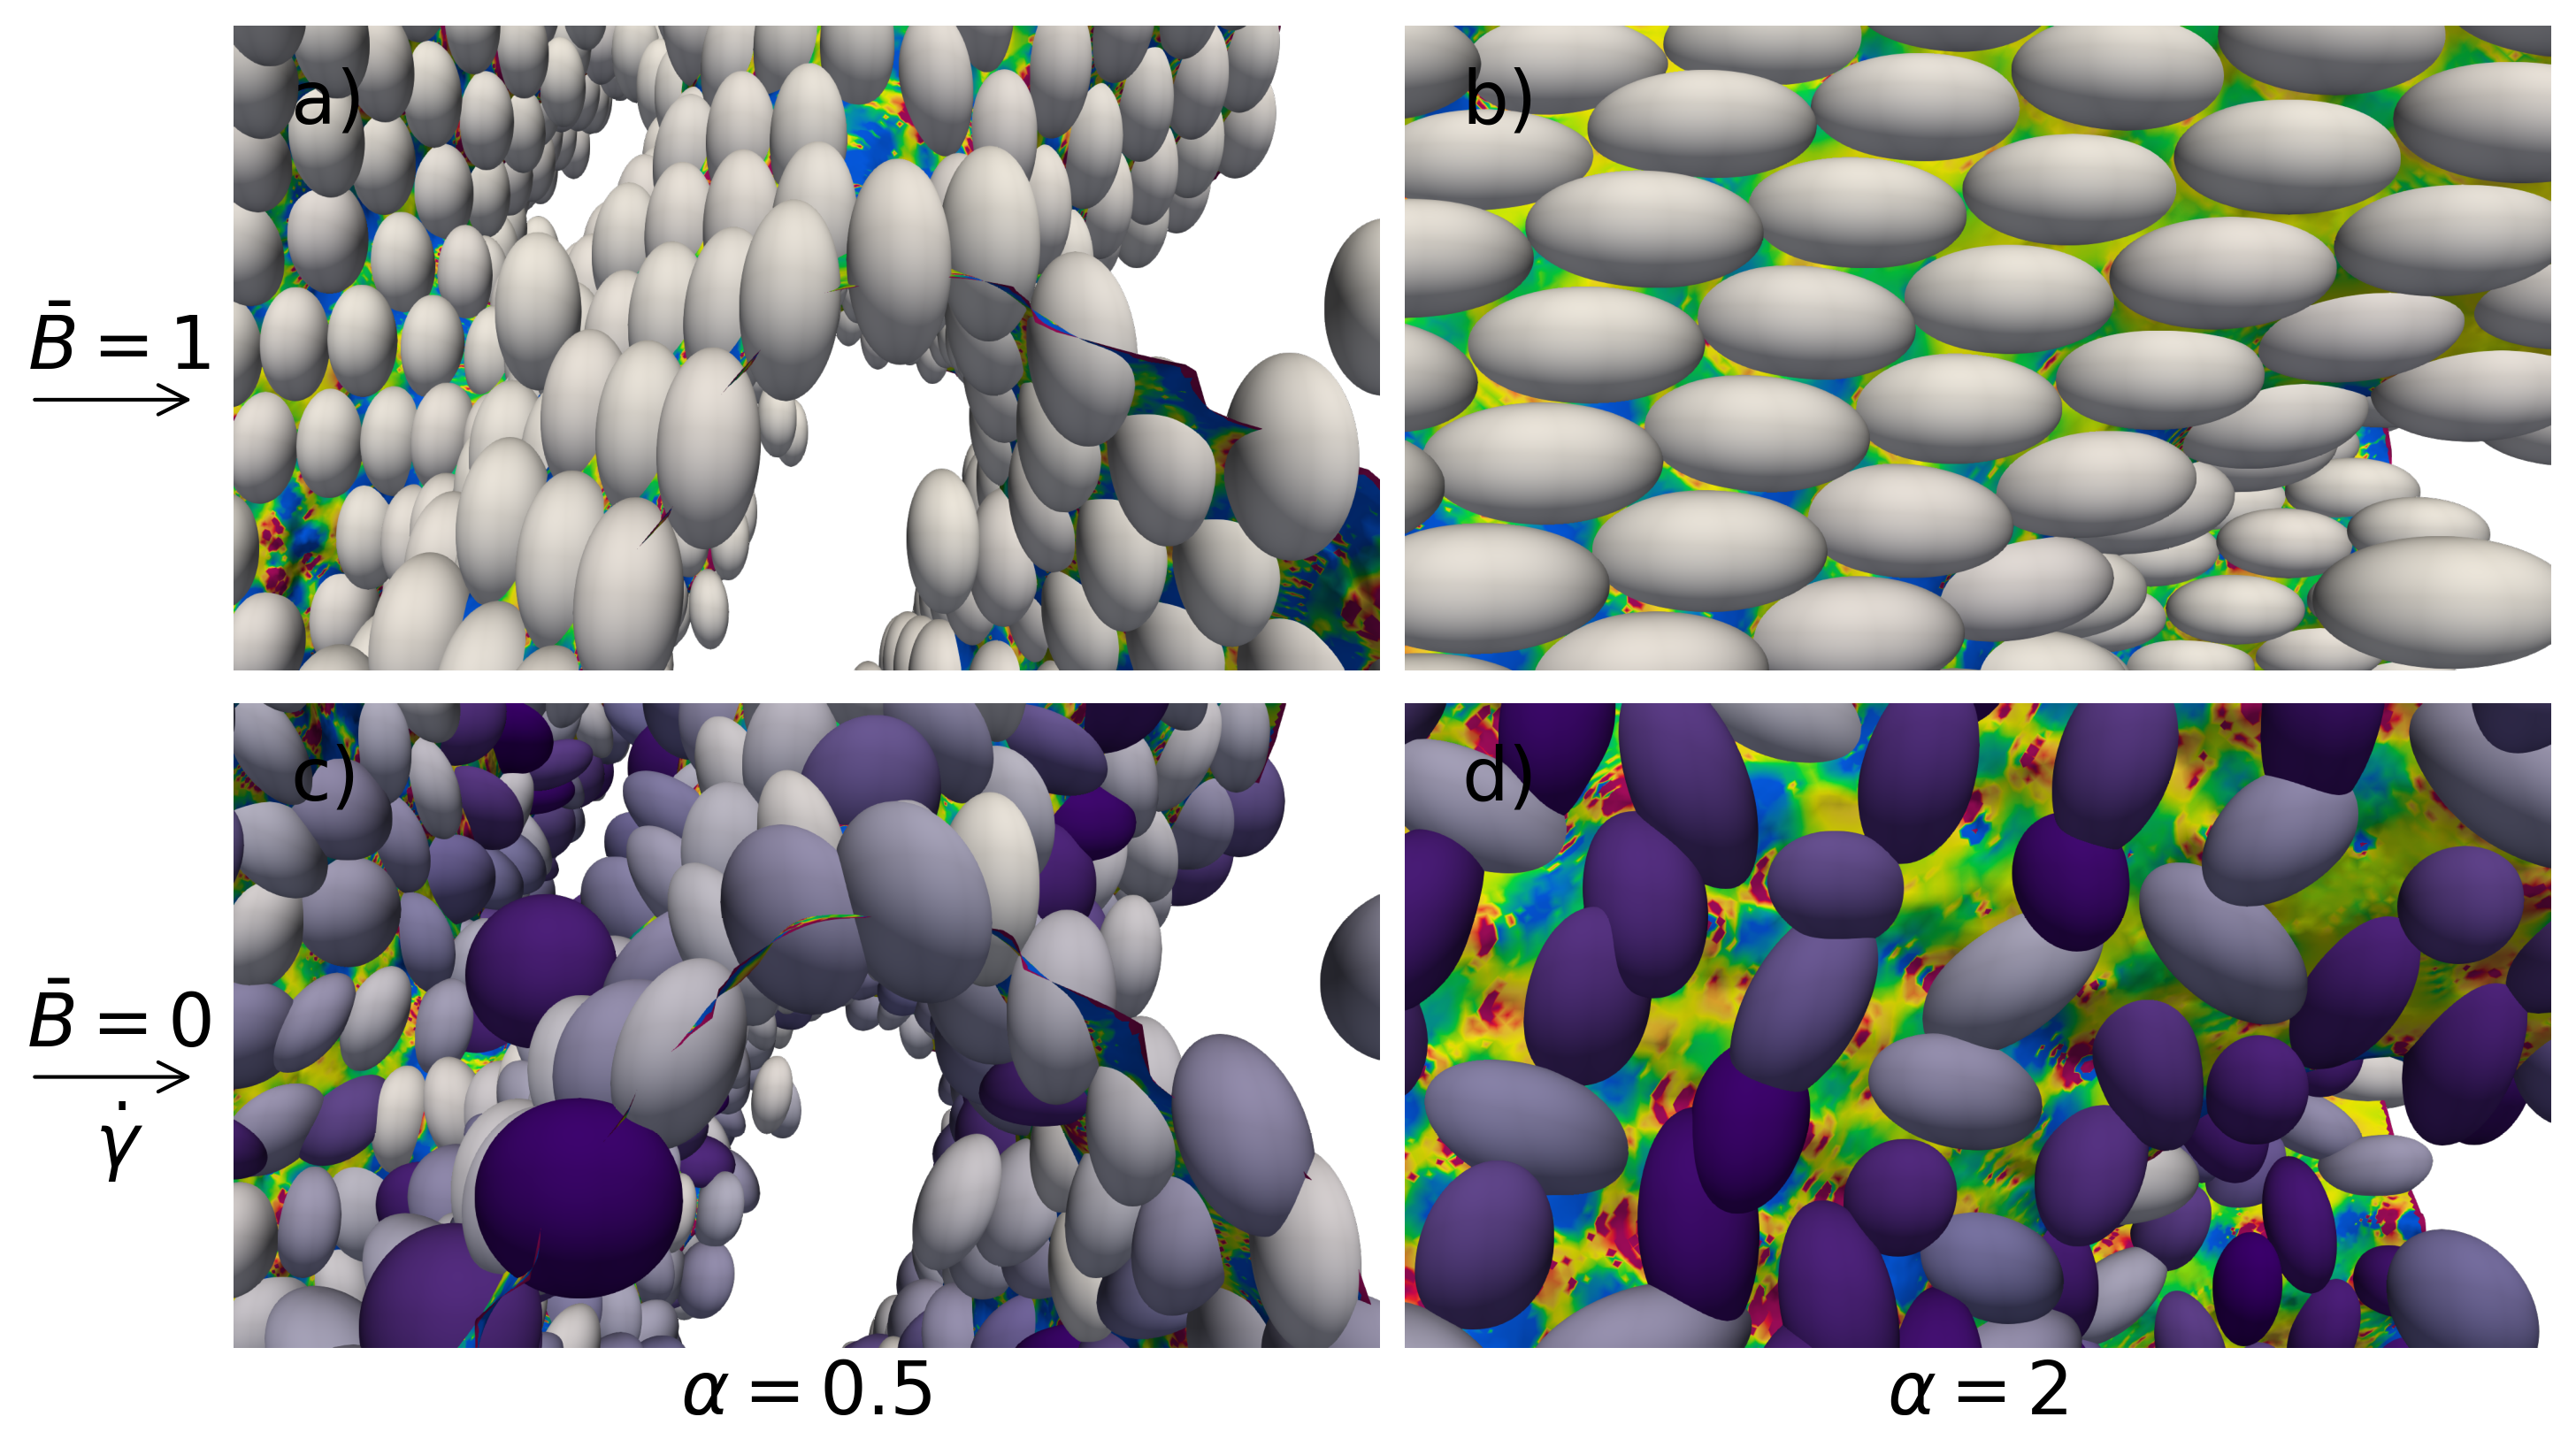
\includegraphics[scale=0.4]{../figures/results/paper3/tz_concat_startB-1_endB-0.png} 
    \caption{Visualization of the particle monolayer of bijels stabilized by prolate and oblate ellipsoidal particles with processing history $\bar{B}: 1 \rightarrow 0$
             undergoing an applied shear of $Ca_s = 10^{-6}$. Particles with a deeper purple shade have a larger angle to the z axis. The top row shows the initial 
             configuration of the particles while the bottom row shows the final configuration of the particles. } 
    \label{fig:particle_viz_tz} 
\end{figure}

In Figure \ref{fig:particle_viz_tz}, the particles are initially ordered to the direction of the applied magnetic field. Upon application of shear and removal
of the magnetic field, I see that the particles begin reorienting away from the z direction. I also observe that the reorientation of particles uncovers the interface.
The reorientation observed is particle morphology specific with prolate particles seeing more reorientation away from the applied shear direction than oblate particles.
Looking at the images, I see that prolate particles rotate away from the direction of the magnetic field and applied shear towards the direction of the shear gradient,
while oblate particles reorient towards minimizing area to the applied shear direction. While these snapshots show the initial and final orientations of the particles at the
interface, we can characterize the time evolution of the particle monolayer changes to identify its role in the rheological properties characterized.

\subsection{Particle properties}

Particles at the interface of bijels stabilized with ellipsoidal particles reorient at the interface to minimize interfacial and
steric energies. \cite{gunther_timescales_2014} The particles stabilizing bijels in confined systems under shear have been shown to
orient to the direction of shear and ejected from the interface at sufficiently long times or shear.\cite{bonaccorso_shear_2020} 
I probe these aspects of the particle monolayer in this section. I plot the orientation of the particle to each cartesian axis 
to identify if I characterize shear induced ordering.

\begin{figure} 
    \centering 
    \includegraphics[scale=0.3]{../figures/results/paper3/angle_to_cartesian-SS.png} 
    \caption{Comparisons of the initial and final particle orientations of the particles to each cartesian direction under
             four processing histories for bijels stabilized with oblate and prolate ellipsoids at multiple shear rates. I show
             shear dependent ordering of the particle monolayer if the initial particle monolayer begins with particle order.} 
    \label{fig:particle_orientation_cartesian_shear} 
\end{figure}

From Figure \ref{fig:particle_orientation_cartesian_shear} I see that with bijel templates simulated under $\bar{B} = 0$, the
particles adopt a random orientation. Upon application of shear, I see that there is little directional ordering to the 
shear direction in the simulation time observed. Upon application of the magnetic field in the $\bar{B}:0 \rightarrow 1$ case, 
the particles order to the direction of the magnetic field. Here we see that the prolate particles order more readily to the applied
field than the oblate particles, seen as a larger clustering of particles at the $\theta_z = 0$ corner of the triangle. In the 
$\bar{B}:1 \rightarrow 0$ case particle morphology dependent partial relaxation of the particles away from the magnetic field direction 
is observed. Directionality of the particles to the field is still observed, suggesting that the ordering of the particles is not
immediately removed once the field is switched off. In the processing history of $\bar{B}:1 \rightarrow 1$, particles are locked
into ordering to the magnetic field direction. However we also see that some particles are reoriented away from the field direction
due to the applied shear. Prolate particles have a smaller distribution of particle orientations than oblate particles, suggesting that
the initial orientation and ordering of particles to the shear applied underpin the response observed. As the particles are adsorbed on the 
interface, the orientation of the particles are influenced by a balance between magnetic forces from the field and capillary forces 
from the interface. We can qualitatively calculate the time evolution of the capillary interactions using the interfacial angle.

\begin{figure} 
    \centering 
    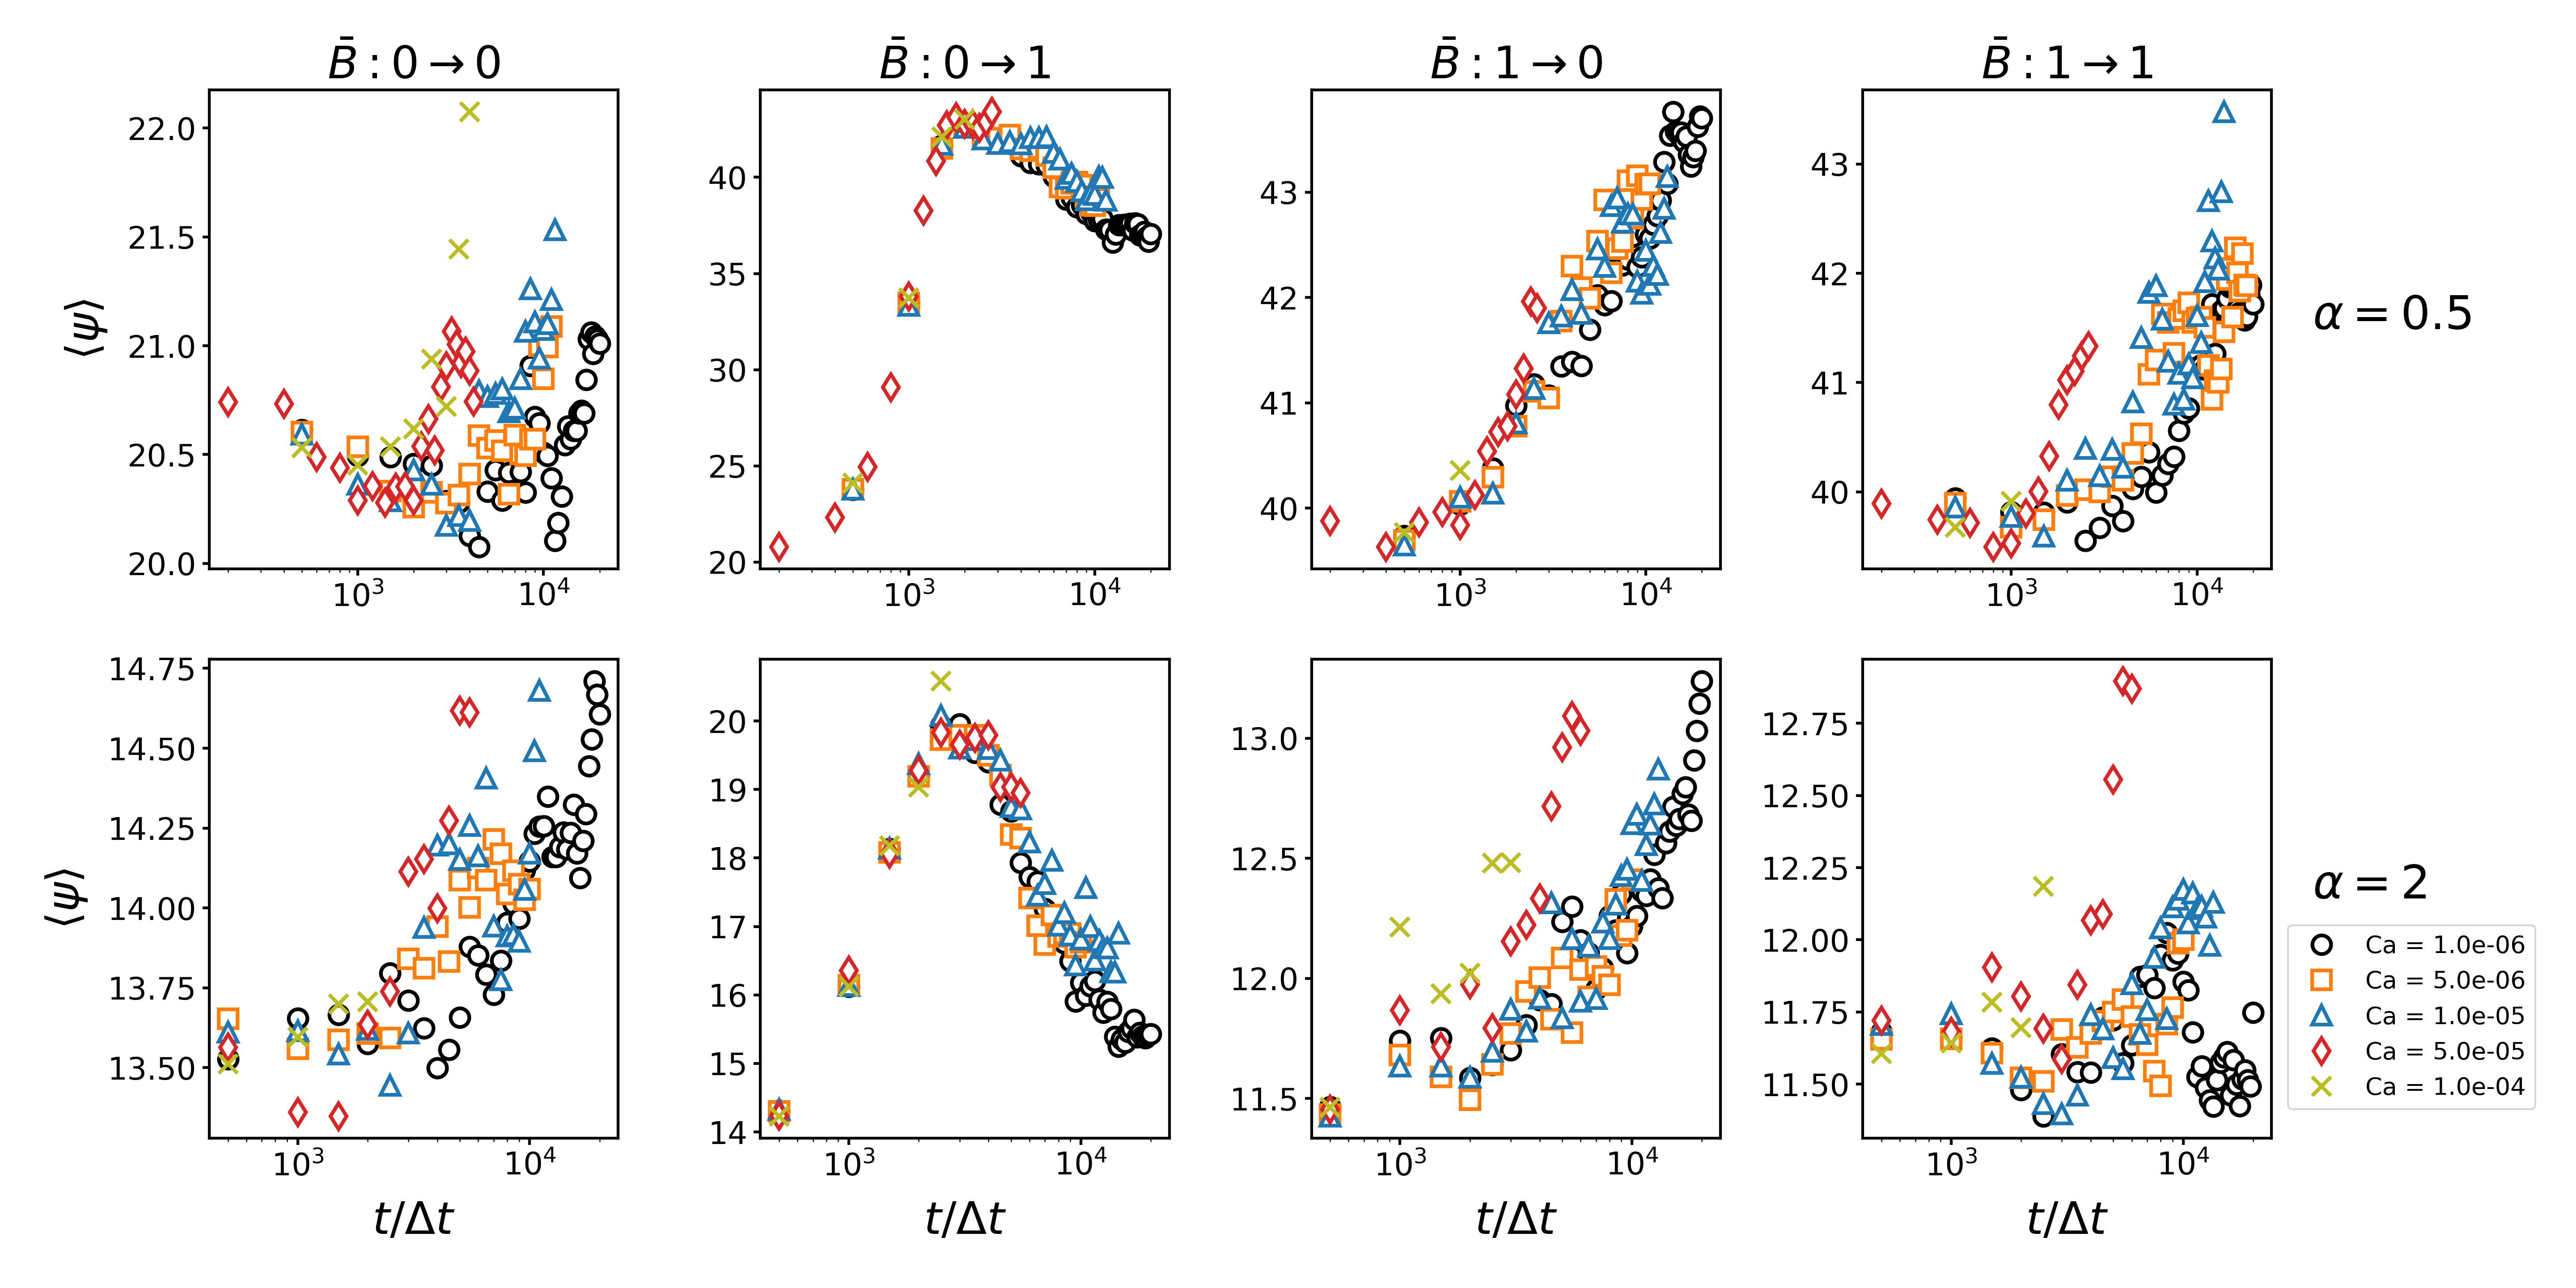
\includegraphics[scale=0.3]{../figures/results/paper3/psi-time_compare.png} 
    \caption{Comparisons of the interfacial angle of bijels stabilized by ellipsoidal particles as a function of 
             the applied shear rate at four different processing histories. I show that upon application of shear
             particles tilt out of the interface reduces the interfacial area stabilized. $\bar{B}: 0 \to 1$ shows 
             large variations in the interface angle.} 
    \label{fig:interface_angle_shear} 
\end{figure}

From Figure \ref{fig:interface_angle_shear}, I demonstrate that there is a slow increase in the interface angle over time for all cases
except for $\bar{B}: 0 \to 1$. For the $\bar{B}: 0 \to 1$ case, this has been shown in Chapter \ref{chapter:aim2} to be due to particle
reorientation to the applied magnetic field. For all other cases, we see an average increase in $\langle \psi \rangle$ over time, showing
that the particles under shear reorient out of the interface. Particles reorienting out of the interface can be due to shear induced interfacial 
stress, modifying the curvature of the interface and thus the lowest energy particle orientation to the interface or shear induced increases in
interparticle forces, causing the particle to tilt out of the interface to minimize interparticle forces. We can characterize the latter 
mechanism through measurements of the number of particles on the interface as increases in interparticle forces result in ejection of
particles from the interface. 

% We can characterize the impact of the interfacial angle on the 
% particle packing using the radial distribution function (rdf).

% \begin{figure} 
%     \centering 
%     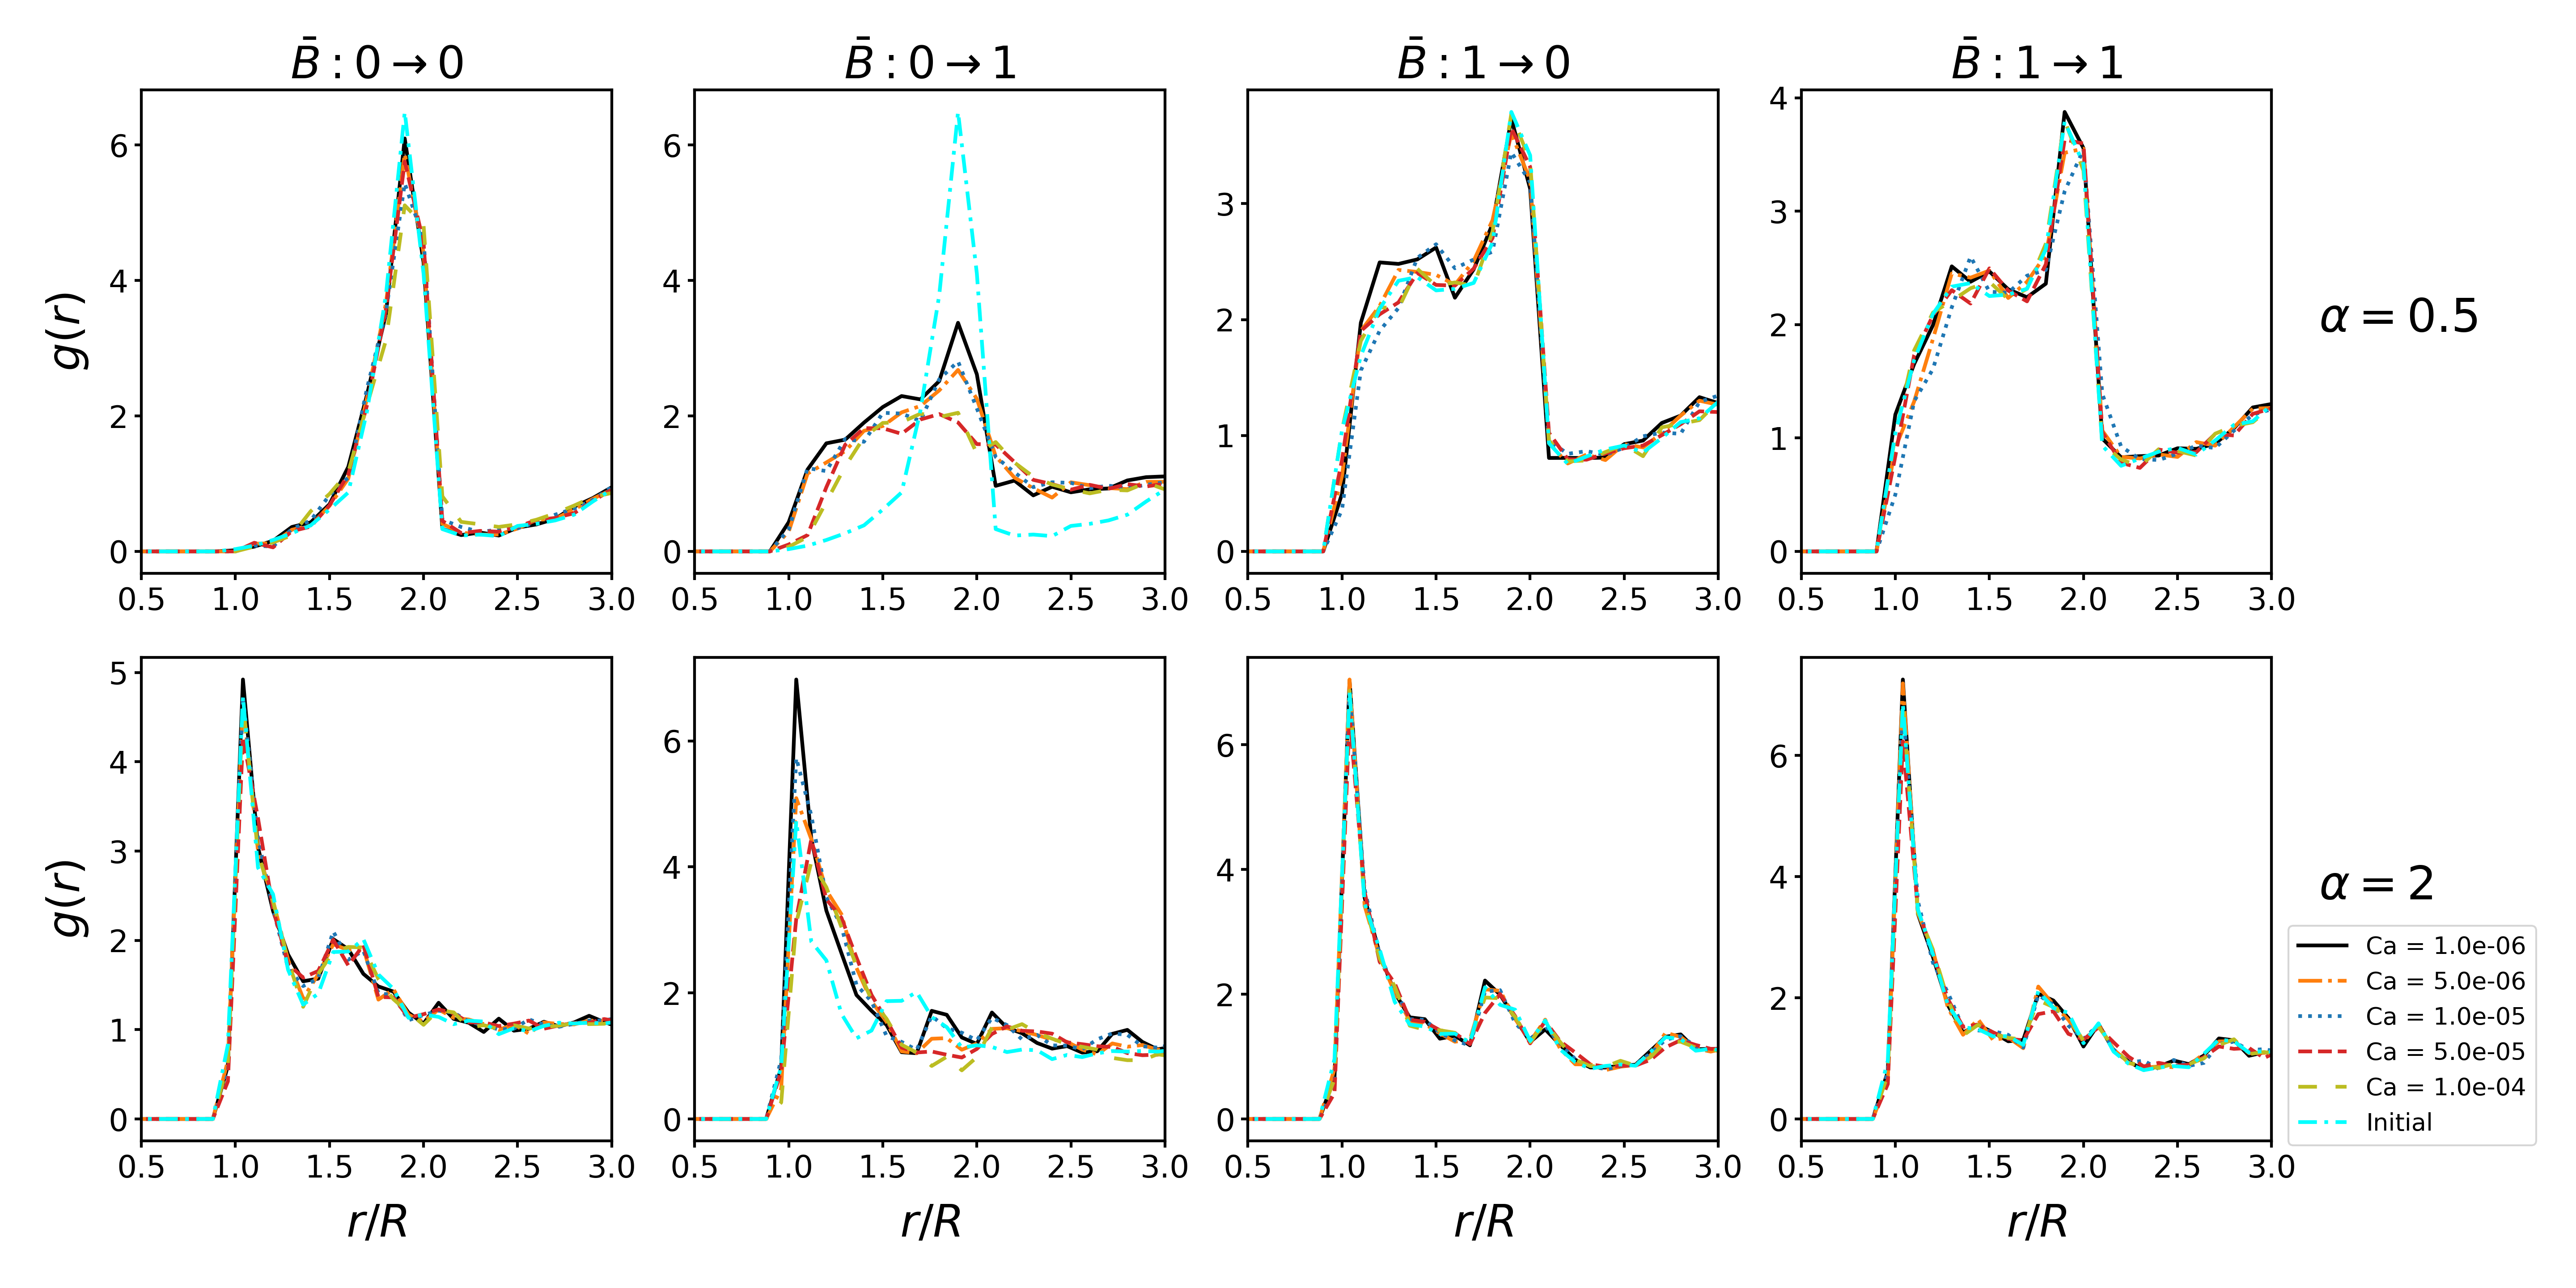
\includegraphics[scale=0.3]{../figures/results/paper3/rdf-SS.png} 
%     \caption{Comparisons of the initial and final radial distribution function of the particles of bijels stabilized by ellipsoidal 
%     particles as a function of the applied shear rate at four different processing histories. I show that there are minor differences
%     in the particle ordering at the interface, suggesting that the particle tilting affects the coverage of particles at the interface.} 
%     \label{fig:rdf_shear} 
% \end{figure}

% From Figure \ref{fig:rdf_shear}, I show that the change in the packing of the particles on the interface is not correlated to the change 
% in the interfacial angle of the particles on the interface when changing the applied field strength in all cases. I then characterize the proportion 
% of particles on the interface to investigate how the proportion of particles on the interface changes and its impact on the interfacial area.

\begin{figure} 
    \centering 
    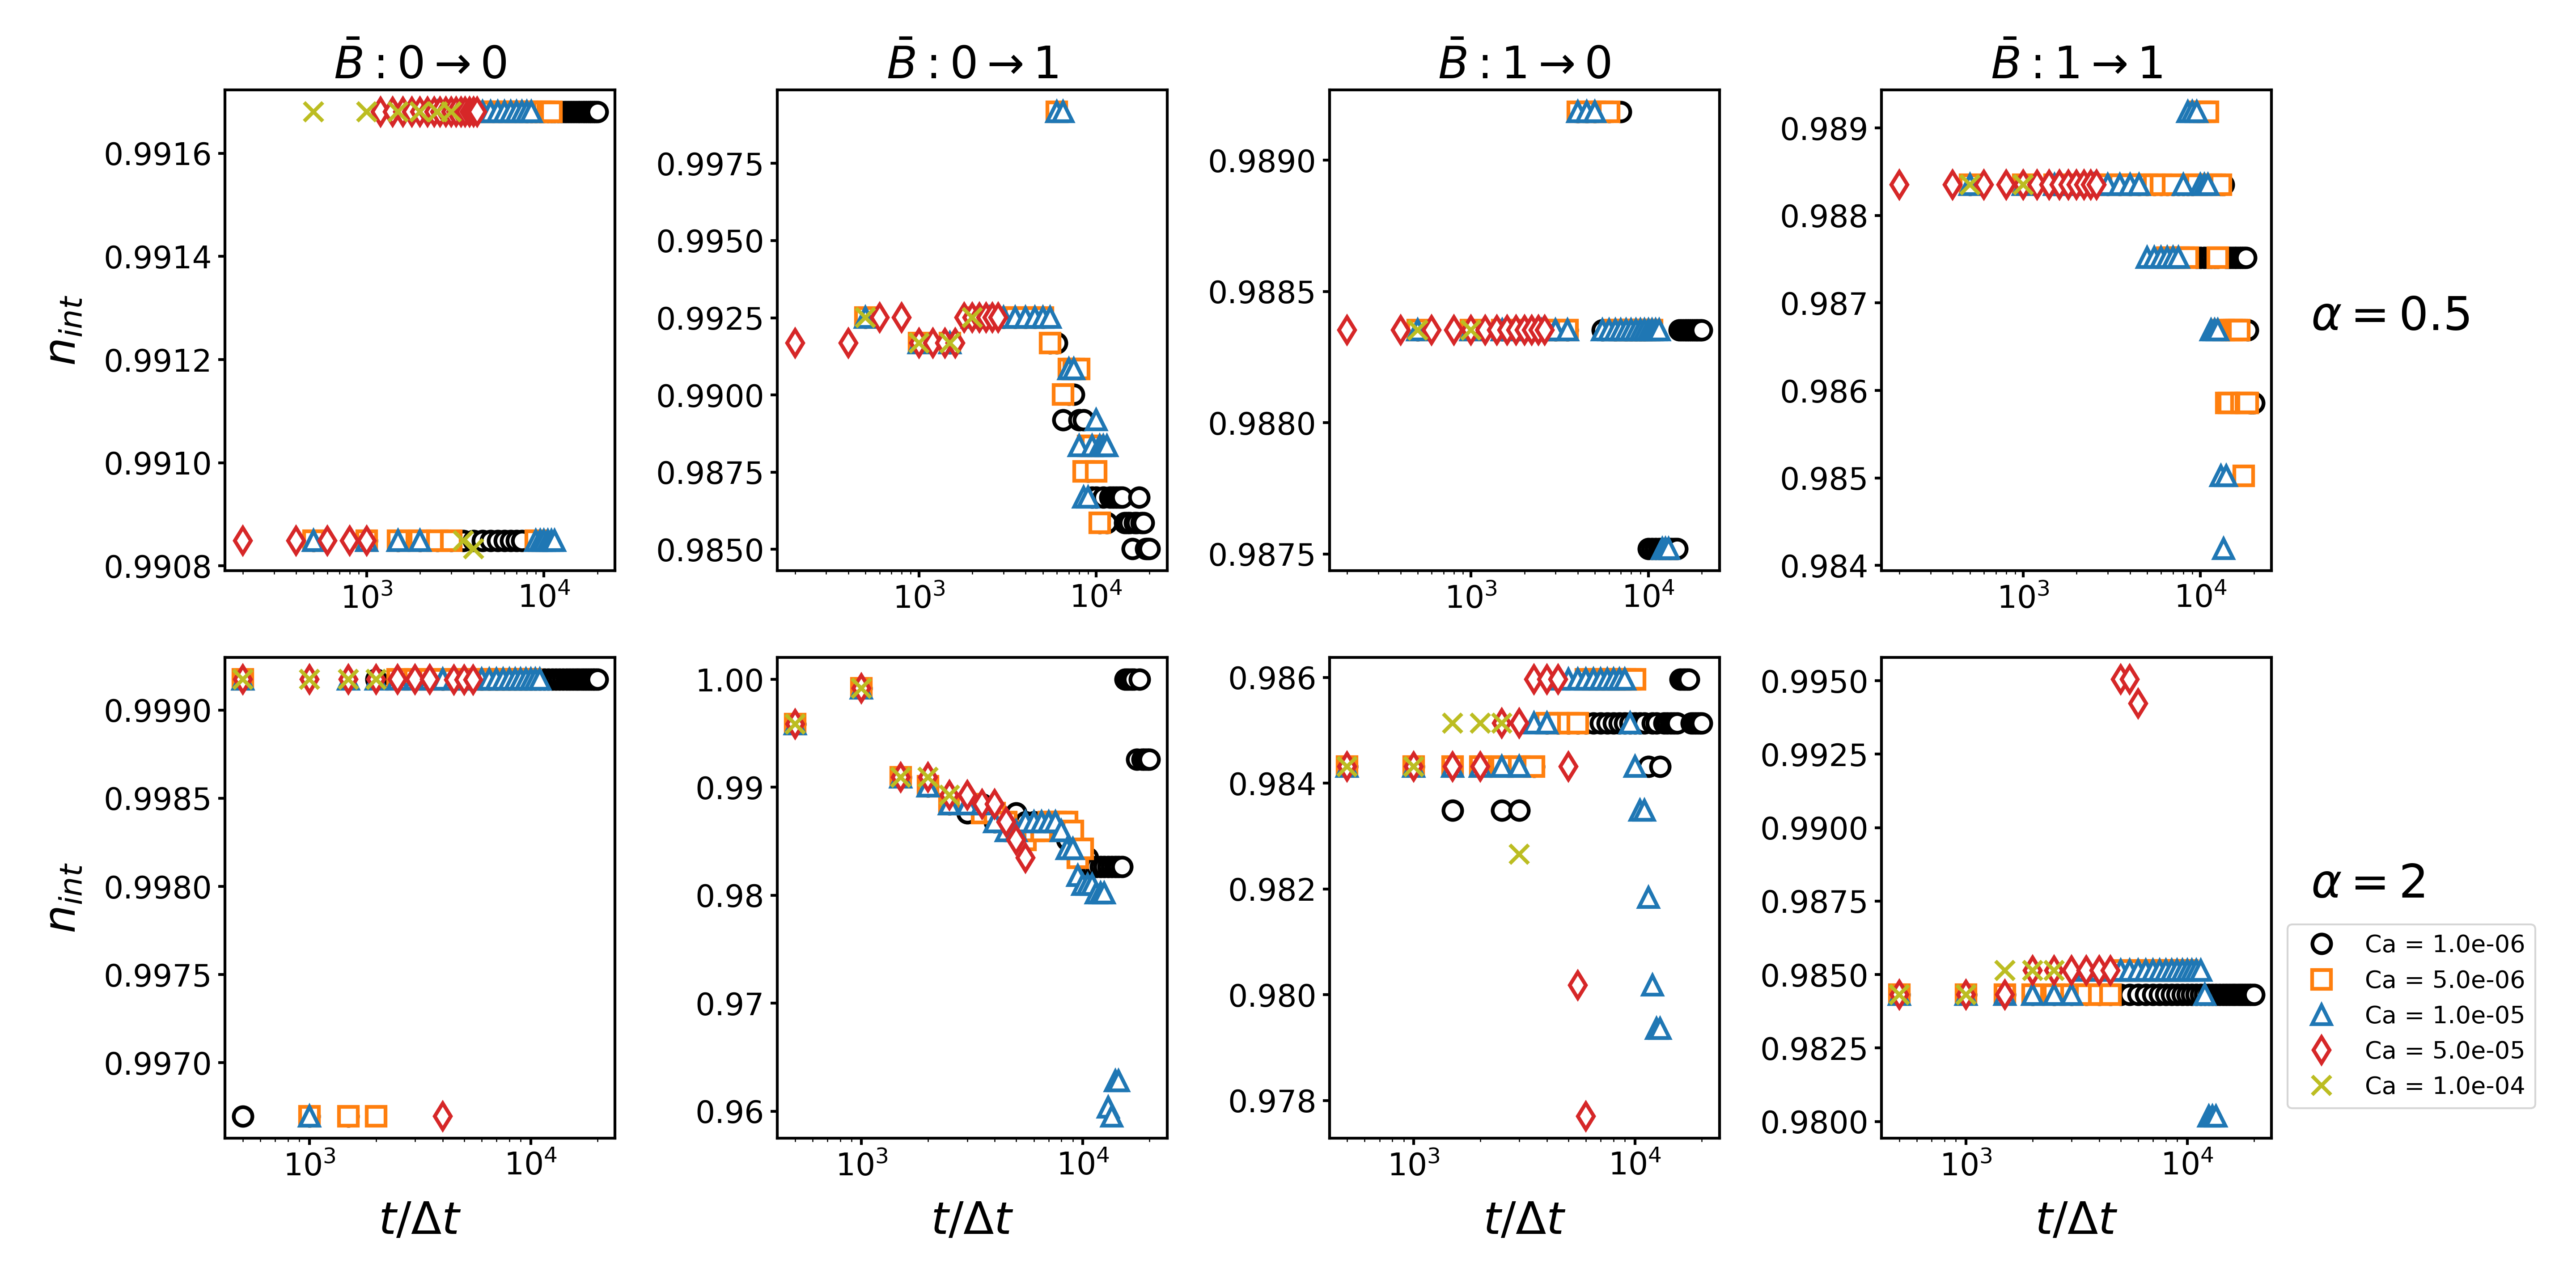
\includegraphics[scale=0.3]{../figures/results/paper3/n_int-time_compare.png} 
    \caption{Comparisons of the proportion of particles on the interface of bijels ($n_{int}$) stabilized by ellipsoidal particles as a function of 
             the applied shear rate at four different processing histories. I show that upon application of shear, many cases have a 
             reduction in the number of particles on the interface while in others it stays the same. For cases where $n_{int}$ reduces, I can 
             attribute the domain size coarsening to this effect.} 
    \label{fig:particles_interface_prop_shear} 
\end{figure}

From the results in Figure \ref{fig:particles_interface_prop_shear}, the impact of the initial microstructure on the number of particles on the interface
differs for bijels stabilized by oblate and prolate ellipsoids. We split this analysis on processing history. While keeping the applied magnetic field
the same, we see little differences in the behavior of $n_{int}$, with their behavior corresponding to changes in $\langle \psi \rangle$. 
Looking at the case of $\bar{B}:0 \rightarrow 0$, there is little change in the number of particles at the interface upon application of shear. This implies that the 
particles remain strongly adsorbed on the
interface. The $\langle \psi \rangle$ results also show this as we see this parameter increasing slowly. This suggests that the particles remain firmly adsorbed
on the interface. Looking to the $\bar{B}:0 \rightarrow 1$ case, the number of particles at the interface drops while $\langle \psi \rangle$ increases. This
trend affects both particles which suggests that shear can pull particles out of the interface due to the decreased
interfacial adsorption energy the particle experiences when rotating out of the interface to orient to the applied field. The $\bar{B}:1 \rightarrow 1$ and 
$\bar{B}:1 \rightarrow 0$ have strong dependences on particle morphology. While an increase in $\langle \psi \rangle$ can be seen in both processing histories 
for both particle morphologies, a decrease in $n_{int}$ can be seen for prolate particles with processing history $\bar{B}:1 \rightarrow 0$ and for 
oblate particles with processing history $\bar{B}:1 \rightarrow 1$. We visualize $\langle \psi \rangle$ at the initial and final timestep for bijels stabilized with
oblate and prolate particles with processing $\bar{B}:1 \rightarrow 0$.

\begin{figure} 
    \centering 
    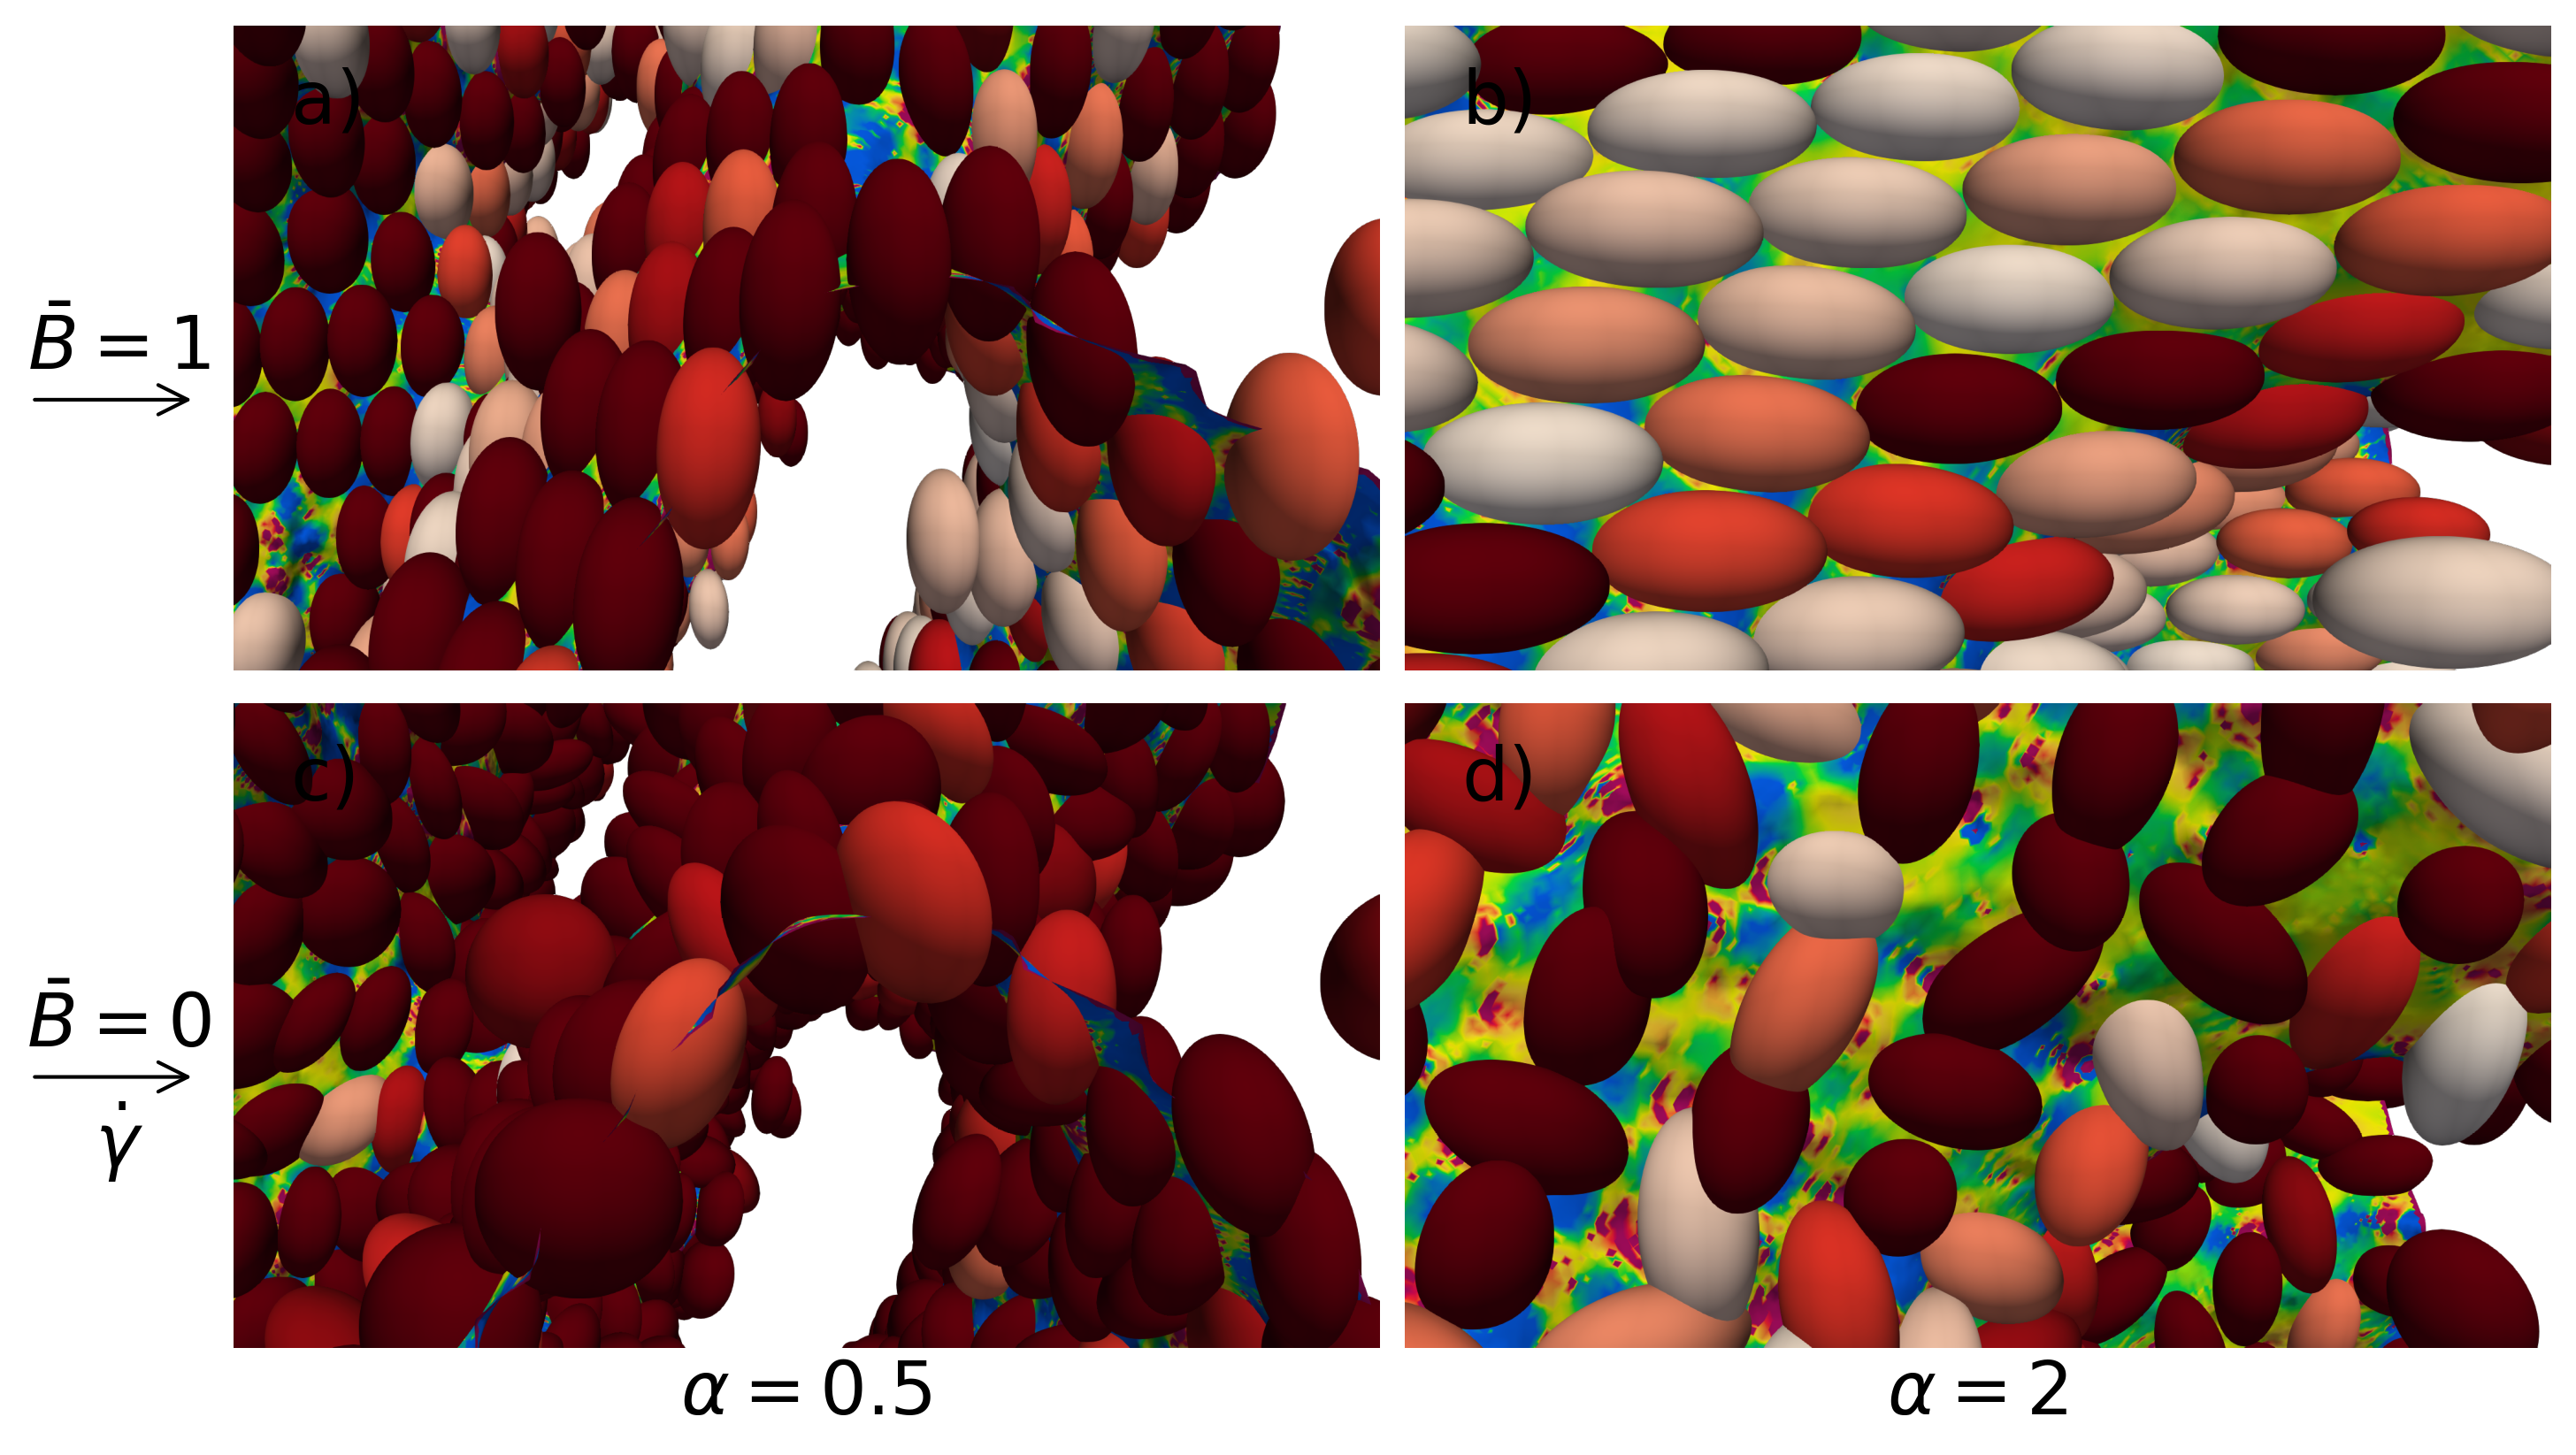
\includegraphics[scale=0.4]{../figures/results/paper3/psi_concat_startB-1_endB-0.png} 
    \caption{Visualization of the particle monolayer of bijels stabilized by prolate and oblate ellipsoidal particles with processing history $\bar{B}: 1 \rightarrow 0$
             undergoing an applied shear of $Ca_s = 10^{-6}$. Particles with a deeper red shade have a larger angle to the interface. The top and bottom row show the 
             configuration of the particles at the initial and final timestep respectively.} 
    \label{fig:particle_viz_psi} 
\end{figure}

Figure \ref{fig:particle_viz_psi} shows that the increase in $\langle \psi \rangle$ seen in Figure \ref{fig:interface_angle_shear} occurs due to different
reasons for both particle morphologies. For oblate particles, this is caused by particles orienting such that their symmetry axis is parallel to the interface
while prolate particles experienced interparticle forces induced by the applied shear, resulting in particles being ejected from the interface when the magnetic 
field is switched off. When keeping the magnetic field on, the oblate particles are forced to stay in sub-optimal particle orientations to the interface, resuling
in ejection of particles from the interface. The presence of the magnetic field reduces shear induced interparticle interactions owing to the ordering of
particles to the applied field, resulting in the mostly unchanged $n_{int}$ values. A increase in $\langle \psi \rangle$ and decrease in $n_{int}$ indicates domain
can indicate coarsening of the fluid domains as the interfacial area is reduced. In the next section, I investigate the the role of the interface properties and the 
impact of particle ejection and tilting of particles out of the interface on the microstructure of bijels.

\subsection{Microstructure change}

Bonaccorso et al. identified that the spherical particle stabilizers in their bijel simulations oriented to the direction of shear before being
ejected from the interface. \cite{bonaccorso_shear_2020} This then led to the domains of the bijel to coalesce and eventually destruction of the
bicontinuous microstructure. \cite{bonaccorso_shear_2020} In our bijels, we characterize particle morphology and initial microstructure specific 
properties of the particle monolayer upon application of shear. 
In this section, I probe the effect of applied shear to the microstructure of magnetically
responsive bijels stabilized by ellipsoidal particles. To investigate the effect of the particle angle and the interfacial coverage of the bijel on the
microstructural evolution of the interface, I plot the area averaged gaussian curvature over time. This parameter will allow insight into the evolution 
of the interface, namely the presence of domain coarsening, coalscence or break-off events.

\begin{figure} 
    \centering 
    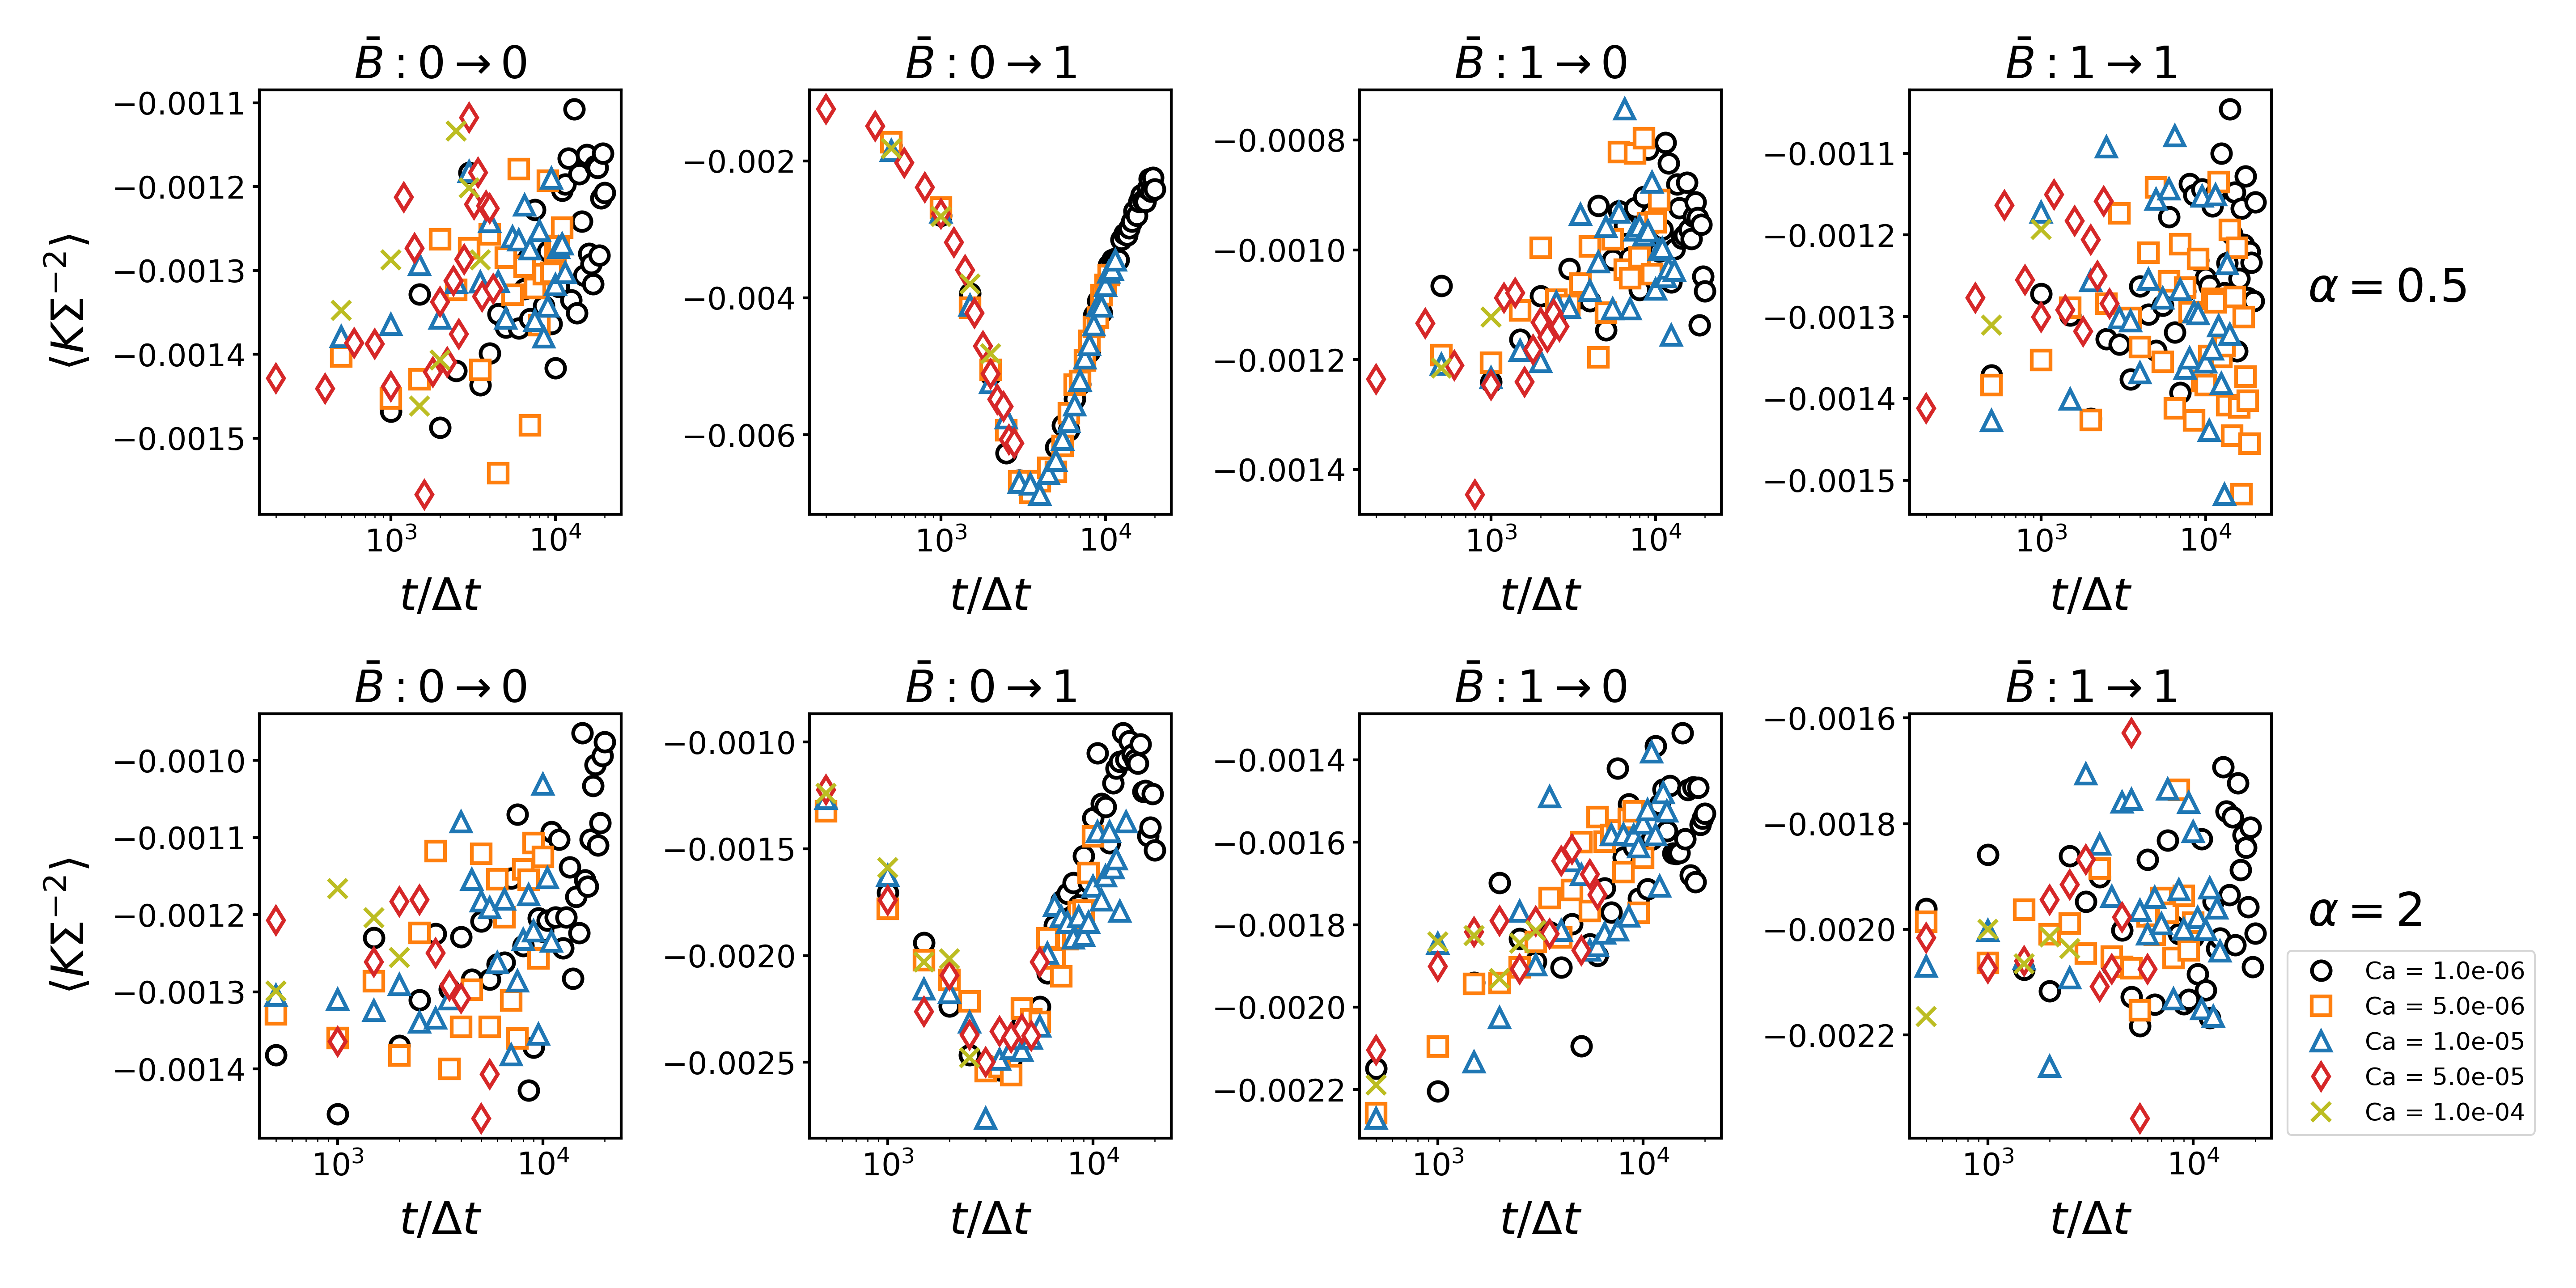
\includegraphics[scale=0.3]{../figures/results/paper3/gaussian-time_compare.png} 
    \caption{Plots of the time evolution of the area averaged Gaussian curvature $\langle K \Sigma^{-2} \rangle$ for four 
             processing histories applied to bijels stabilized with oblate and prolate ellipsoids. I demonstrate that the 
             magnitude of the gaussian curvature reduces for all systems except for $\bar{B}: 0 \to 1$.} 
    \label{fig:gaussian_curvature_time_shear} 
\end{figure}

Figure \ref{fig:gaussian_curvature_time_shear} reveals that the area averaged Gaussian curvature generally decreases in magnitude over time for all cases except 
$\bar{B}: 0 \to 1$ indicating that the increase in $\langle \psi \rangle$ causes domain coarsening of the bijel. $\bar{B}: 0 \to 1$ is
unique because particle rearrangements at the interface dominates the dynamics of the microstructure, not observed in all other
cases. From the time evolution of the curvature, the same mechanism drives coarsening in all cases. From the results in Figures \ref{fig:particles_interface_prop_shear} 
and \ref{fig:interface_angle_shear}, domain coarsening is driven through a reduction in the interfacial area covered by the particle monolayer. 
From the curvature results characterized in Figure \ref{fig:gaussian_curvature_time_shear}, the area averaged curvature coarsening is shear independent. This is further
evidence that the mechanism of coarsening is identical in each case. 

\begin{figure} 
    \centering 
    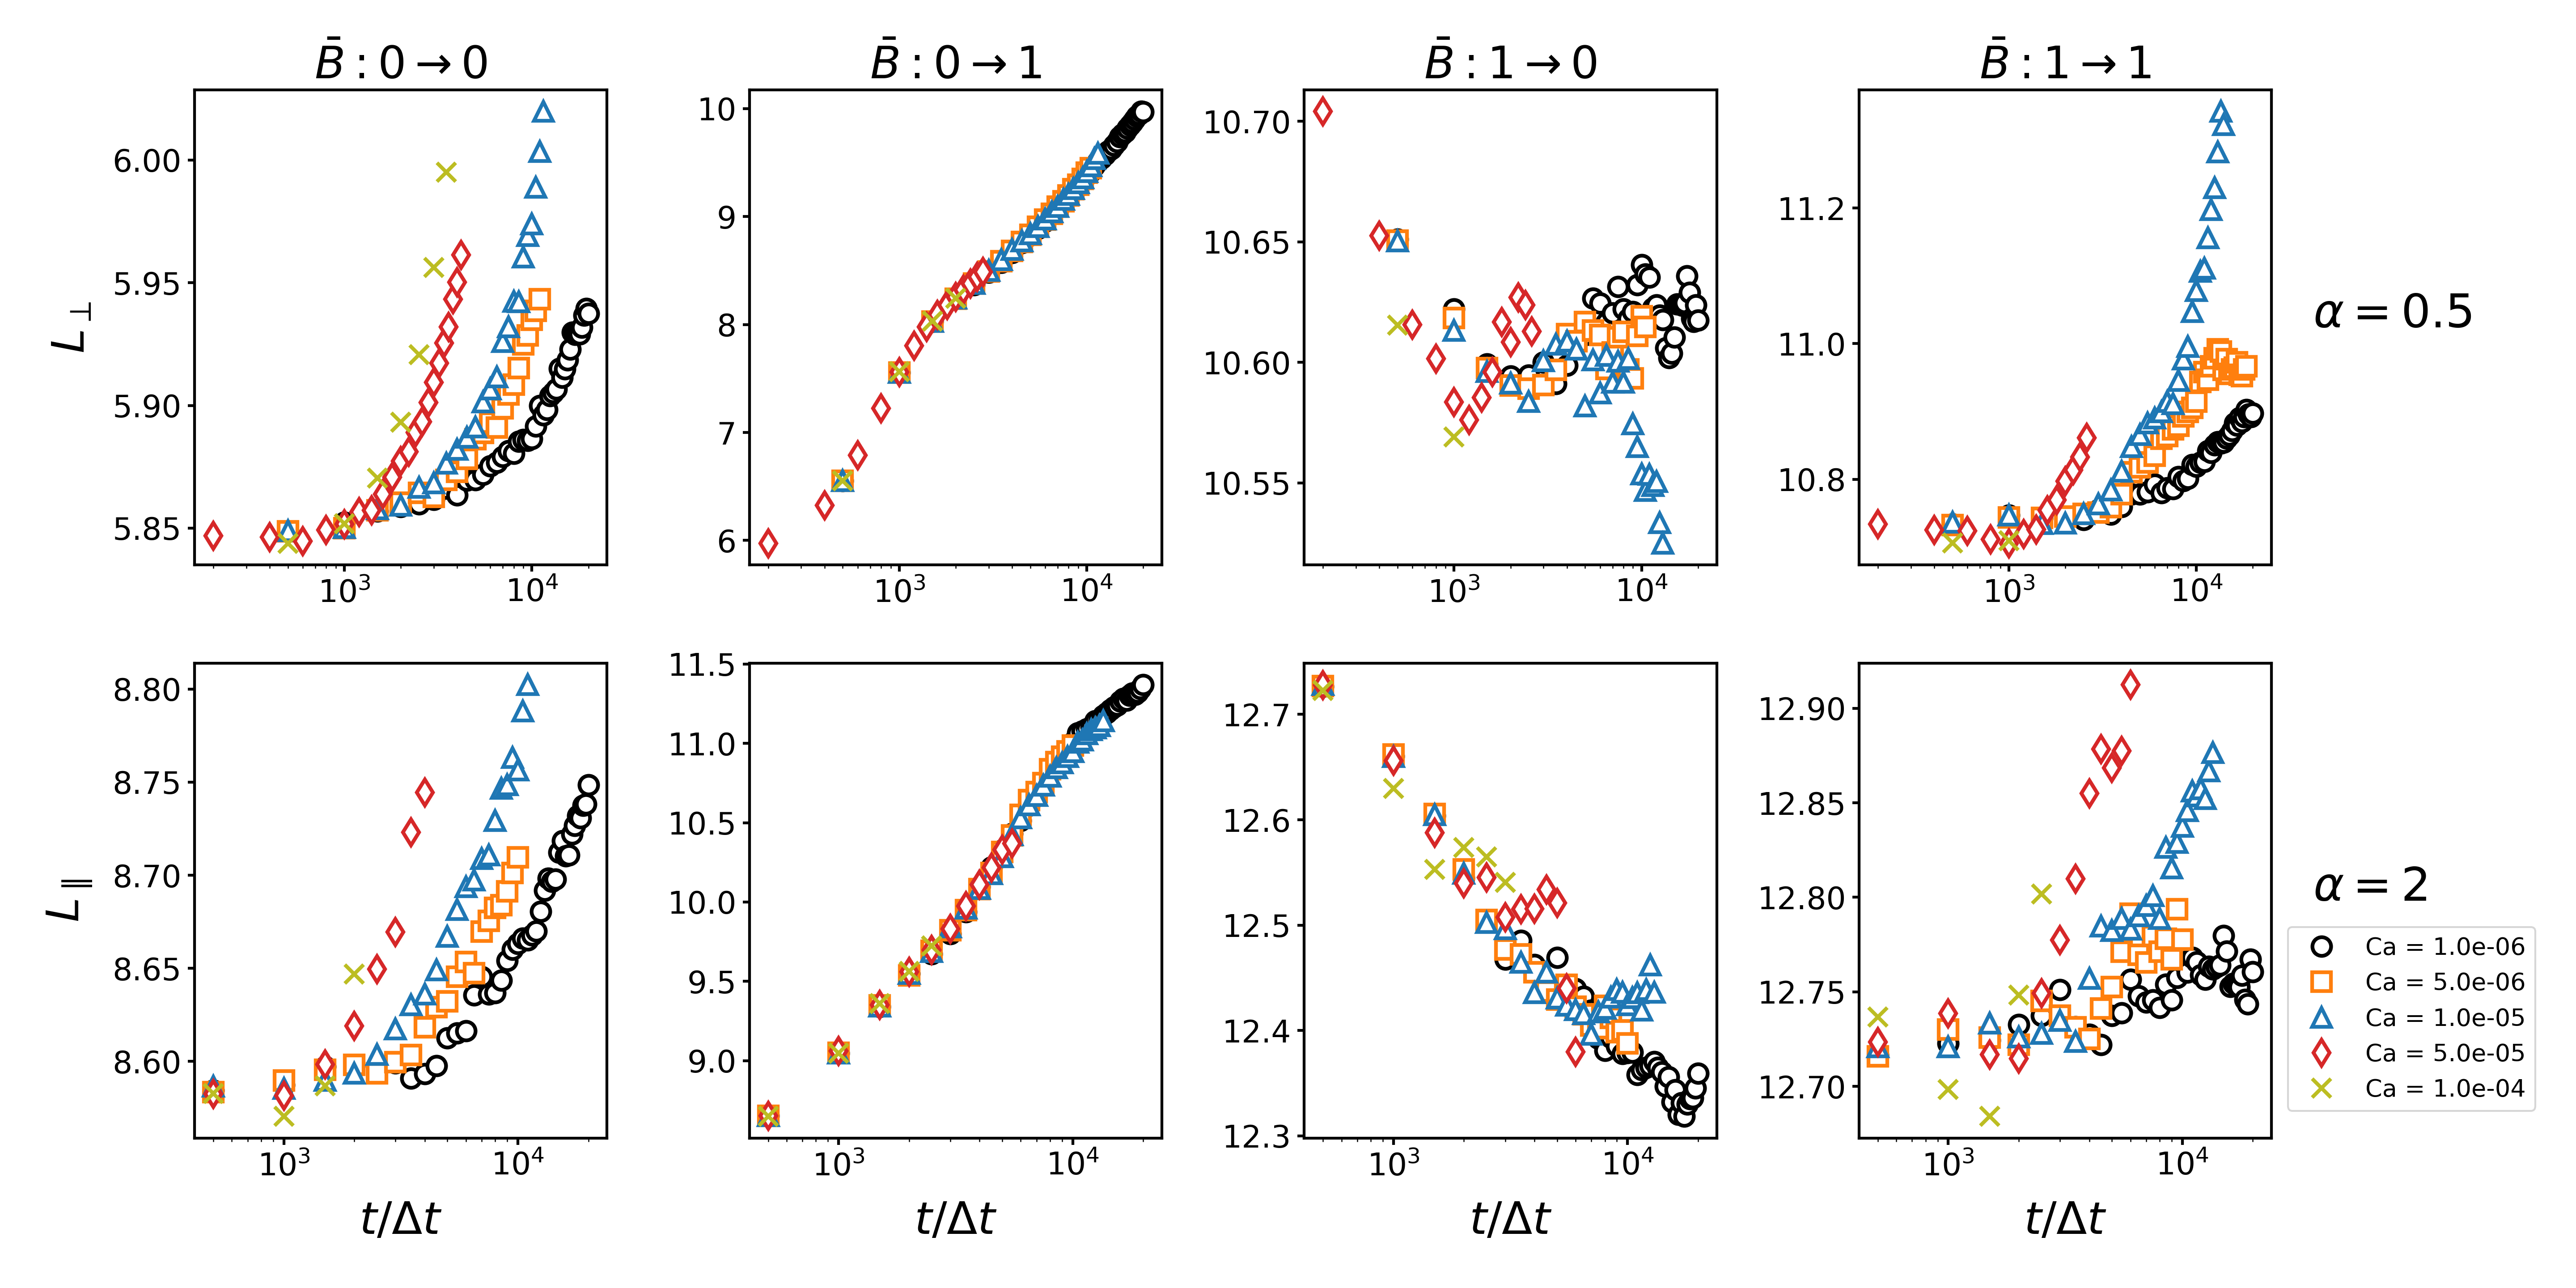
\includegraphics[scale=0.3]{../figures/results/paper3/anisotropy_compare.png} 
    \caption{Comparisons of the time evolution of the directional domain sizes that increase upon application of a magnetic field for bijels stabilized 
             by ellipsoidal particles undergoing various shear rates under four processes. The directional domain size increases in all cases except for when the
             field is switched off.} 
    \label{fig:domain_size_aniso_time_shear} 
\end{figure}

From Figure \ref{fig:domain_size_aniso_time_shear}, the directional domain sizes in the orientations with the maximum change were characterized. For oblate and prolate 
particles, this was found to be $L_{\perp}$ and $L_{\parallel}$ respectively. In all cases except for $\bar{B}: 1 \to 0$, this length scale increases matching the expected
trend that increasing $\langle \psi \rangle$ matches domain coarsening. The decrease in these length scales for $\bar{B}: 1 \to 0$ suggest that the shear induced
reordering of interfacial particles after application of a field affects the evolution of the microstructure. For both particles, this is due to particle mediated
shear forces causing domains to coarsen more in specific directions. From the snapshots of the particle arrangement in Figure \ref{fig:particle_viz_psi} the particles were
shown to reorient at the interface. This process did not occur for $\bar{B}: 1 \to 1$ as the presence of magnetic fields acted to keep particles aligned a specific
direction. 

% Previous investigations have 
% demonstrated how the orientation and arrangement of particles on the interface affect the domain size. 
% \cite{gunther_timescales_2014} I focus our investigation on this aspect in the following plot.

% \begin{figure} 
%     \centering 
%     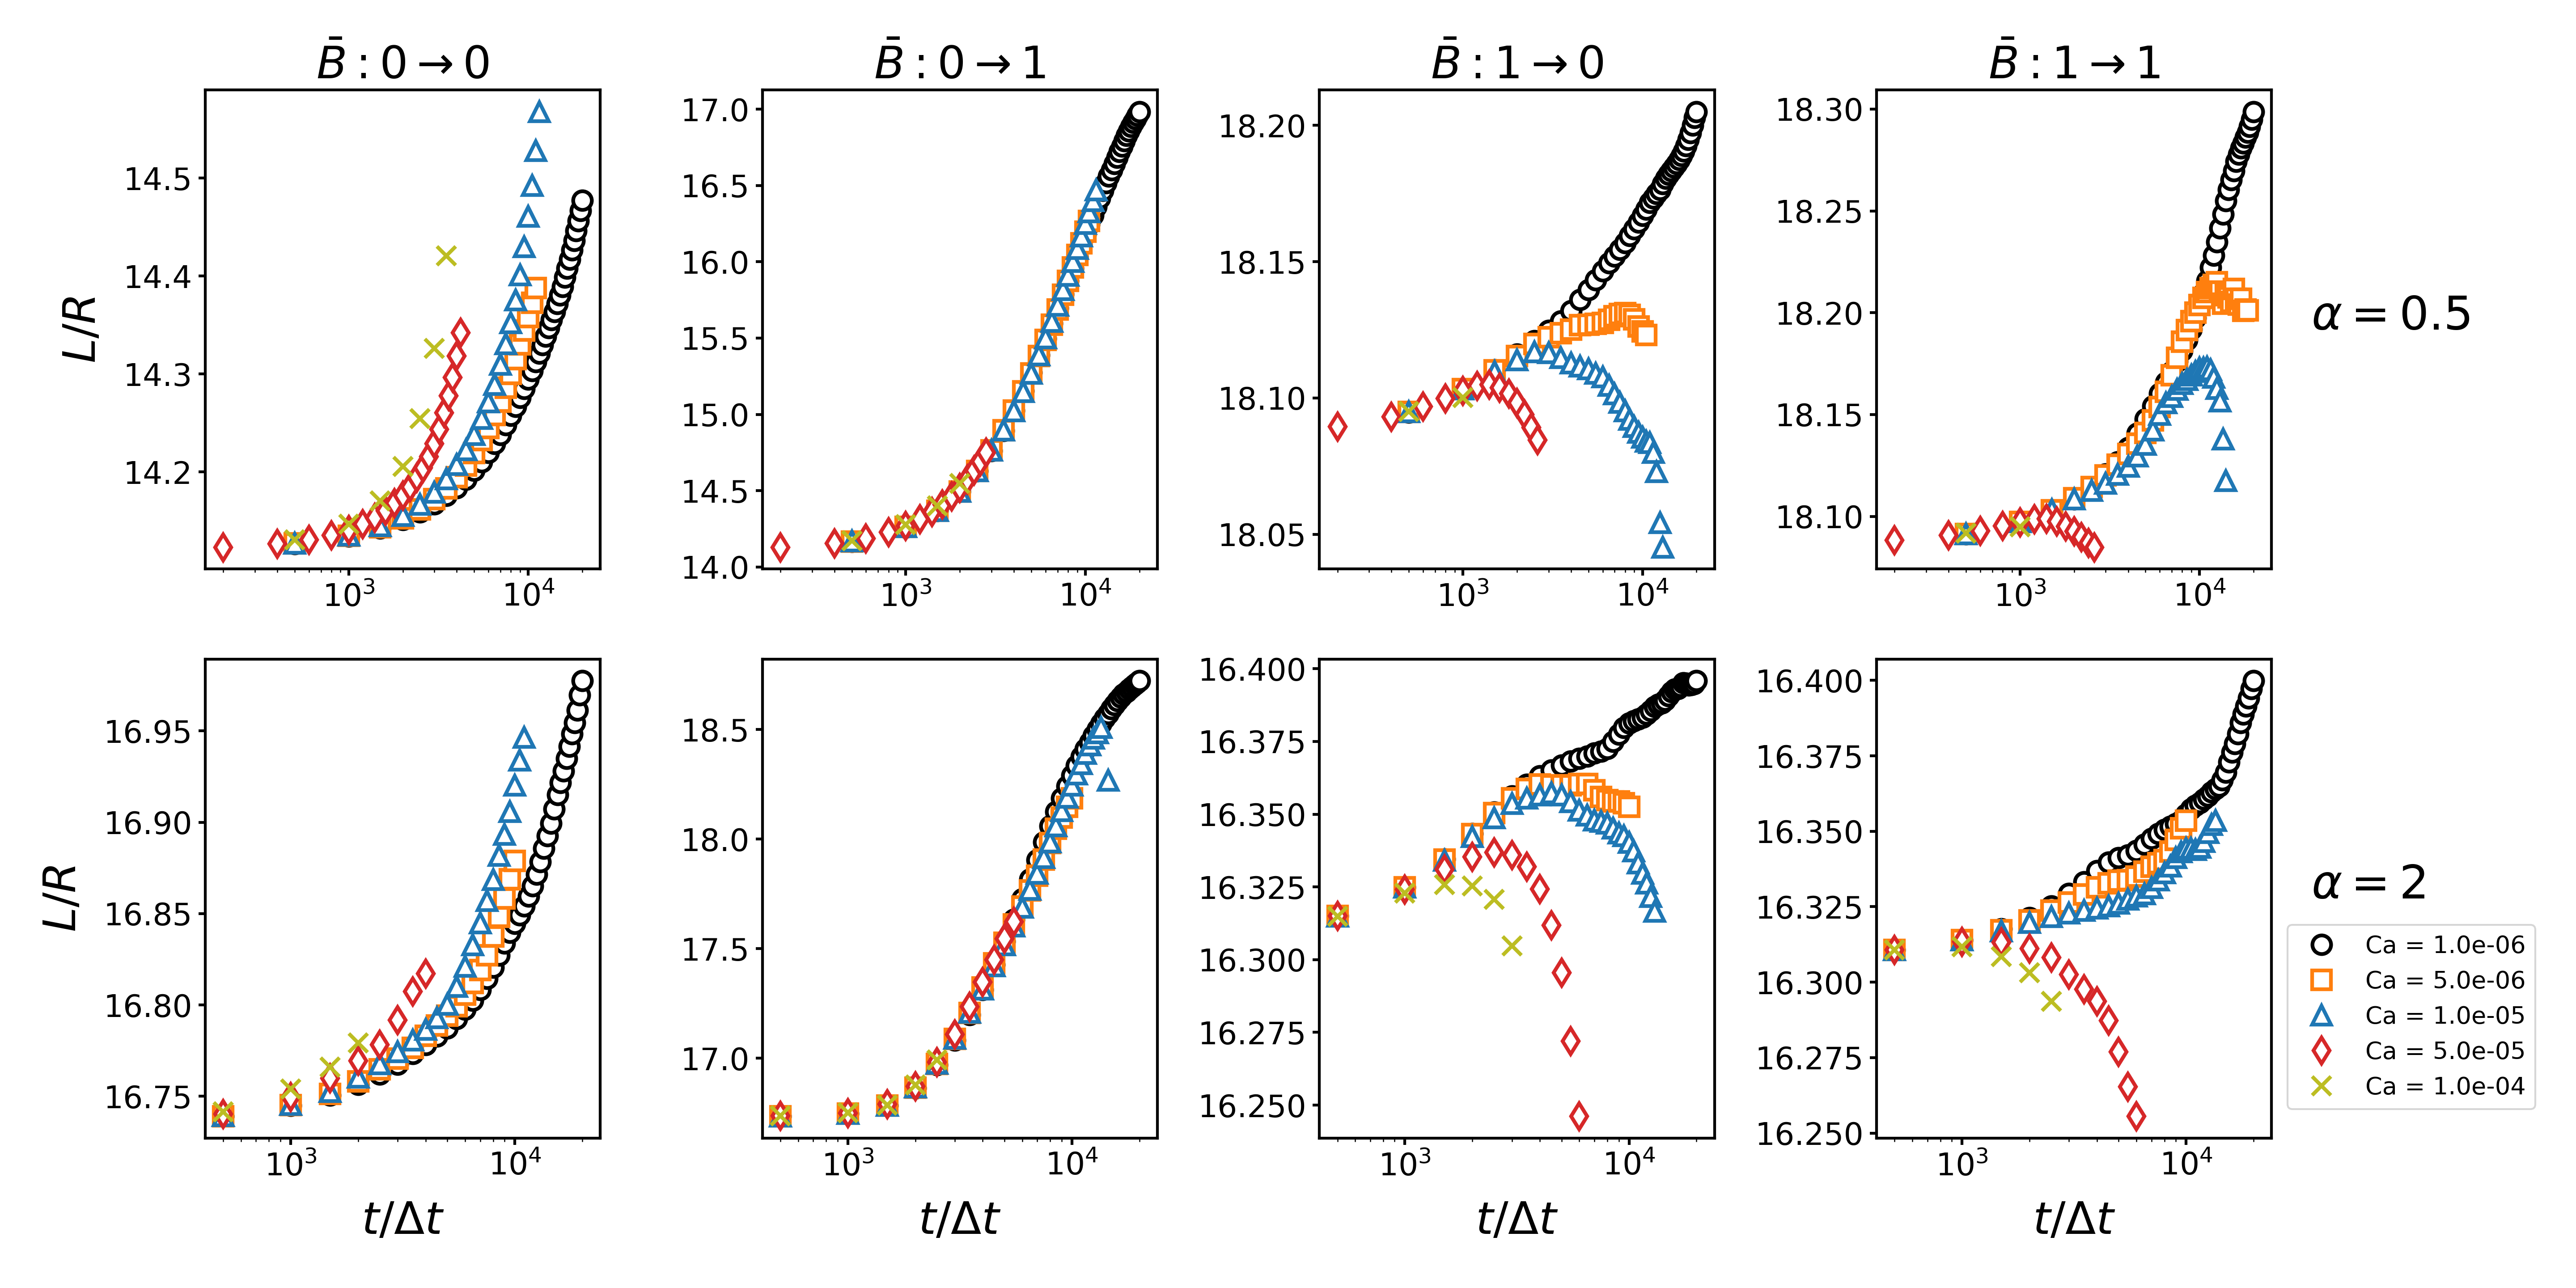
\includegraphics[scale=0.3]{../figures/results/paper3/domain_size-time_compare.png} 
%     \caption{Comparisons of the time evolution of the average domain size for bijels stabilized by ellipsoidal particles undergoing
%              various shear rates under four processes. Initially, the domain size coarsens for all runs under applied shear before
%              reducing in some cases.} 
%     \label{fig:domain_size_time_shear} 
% \end{figure}

% From Figure \ref{fig:domain_size_time_shear}, domains coarsen with time in all cases. When increasing the applied magnetic field in the case of 
% $\bar{B}:0 \rightarrow 1$, I see shear assisted domain coarsening characterized as a 20 \% and 10 \% increase in the domain size of bijels
% stabilized by oblate and prolate particles respectively. This is approximately 5 times greater than the response observed in Figure \ref{fig:domain_size-field_on}
% In the  $\bar{B}: 1 \to 0$ and $\bar{B}: 1 \to 1$ cases, an initial plateau in domain size is observed, followed by a divergence in 
% growth depending on $Ca$. The shear rate appears to influence domain coarsening, with higher $Ca_s$ leading to delayed or 
% suppressed growth, especially in the presence of a field. The difference between applying $\bar{B}: 0 \to 1$ and 
% removing $\bar{B}: 1 \to 0$ the field demonstrates the stability of the particle monolayer when a field is switched off.
% There is little difference in the qualitative trends of domain size change for bijels stabilized with oblate or prolate particles.
% To characterize whether the domain size coarsening observed arises from different phenomena in each case, the area averaged curvature is plotted.

\section{Conclusions}

% In this chapter, I investigated the rheology of bijels stabilized by ellipsoidal particles under shear, focusing on the influence of initial microstructure and the 
% application of a constant magnetic field on their shear response. The shear behavior was characterized using a Herschel-Bulkley fitting function to extract the flow index, 
% consistency index, and yield stress. My analysis confirmed that the shear-thinning nature of bijels remains robust, regardless of particle morphology or applied magnetic 
% field. However, the flow index and yield stress trends were strongly dependent on these factors.  
% I found that increased particle ordering led to distinct yield stress behaviors: oblate particles resulted in a lower yield stress, while prolate particles exhibited a 
% higher yield stress. When examining the properties of the particle monolayer, I identified a clear impact of particle morphology on interparticle interactions at the 
% interface. In the absence of a magnetic field, both particle monolayers remained adsorbed at the interface. However, when a magnetic field was initially applied, the 
% behavior diverged significantly oblate particles flipped out of the interface to minimize interfacial energy, whereas prolate particles tilted out. These differences 
% directly influenced the shear response, altering how the surrounding fluid flows around the particles and leading to the observed non-Newtonian behavior and yield 
% stress characteristics.  
% Furthermore, I investigated the microstructural effects of shear and magnetic field-induced particle ordering and found that coarsening was the primary driver of 
% domain size evolution in sheared bijels. This coarsening was facilitated by a reduction in interfacial particle coverage. When analyzing the anisotropic domain size evolution, 
% I observed that in most cases, the direction of greatest structural change aligned with expected trends—except when the magnetic field was switched off. This deviation is 
% attributed to differences in particle monolayer evolution, depending on whether the bijel was formed with or without an initially applied field.  

The rheological properties of bijels are of importance in many fabrication schemes such as STrIPS and homogenization. \cite{haase_continuous_2015,cai_bijels_2017}
To characterize how magnetically responsive bijels can be used in these synthesis techniques, I studied the effect of particle morphology, initial microstructure and
applied magnetic fields on the rheology of bijels experiencing a constant shear. Bijel templates made with $\bar{B} = 0$ and $\bar{B} = 1$ were selected, with field strengths
of $\bar{B} = 0$ and $\bar{B} = 1$ applied to each template. This results in four processing histories per particle morphology namely $\bar{B}:0 \rightarrow 0$,
$\bar{B}:0 \rightarrow 1$, $\bar{B}:1 \rightarrow 0$ and $\bar{B}:1 \rightarrow 1$. I then apply a constant shear rate onto each bijel.

I first characterized the shear stress imparted by bijels under several strain rates. The shear stress calculated continued to increase in line with expectations
for colloidal glasses as ageing occurs. Thus a pseudo-steady state was selected to compare the shear properties of the bijel.
I fit the shear stress data using a Herschel Buckley fit and identify that the flow index of bijels stabilized by ellipsoidal 
particles under magnetic fields became less shear thinning. The yield stress of bijels stabilized by oblate particles was shown to reduce by 4x while the yield stress
of bijels stabilized by prolate particles was shown to increase by 2x upon application of magnetic fields.

To characterize these differences, closer attention is paid to the particle monolayer of the bijel. Shear induced reorientation of the ellipsoids can be observed in cases
where a magnetic field was used observed, characterized as the orientation of particles drift away from the magnetic field direction. When analyzing the effect this reorientation
has on the particles at the interface, the interface angle in all cases increases as a function of the shear rate. However the quantitative behavior of oblate particles differ
from prolate particles. Under magnetic fields, oblate particles tend to flip out of the interface while prolate particles tilt out of the interface. The impact that
the particle tilting and flipping out of the interface can also be seen in the number of particles in the interface, where the differences in the particle morphology 
can be characterized as differences in the number of particles at the interface in response to the magnetic field. 

A reduction in the number of particles at the interface and the particles tilting out of the interface reduces the interfacial coverage. The reduction in interfacial
coverage manifests as domain coarsening, characterized as a smooth decrease in the magnitude of the area averaged Gaussian curvature. The changes in the particle monolayer
properties manifest as changes in the evolution of the directional domain size evolution due to shear induced particle reorientation at the interface. 

Past literature
has shown how bijels are susceptible to failure when being used as crossflow reactors due to shear induced domain coarsening resulting in microstructure failure. 
\cite{boakye-ansah_controlling_2020} The investigations conducted here demonstrate that controlling the orientations of particles at interfaces are crucial to 
the rheological properties of bijels. Other properties not considered here such as different particle aspect ratios, the effect of surface tension on the shear response of
bijels and the volume fraction of particles are not considered here. Additionally, complex rheology of the bijels can determine detailed rheological properties such as the
gel point and phase difference of the bijel which can yield further rheological characterization of bijels stabilized by magnetically responsive ellipsoidal particles.

% % Extensions to this work can be accomplished by investigating the effect of applying a magnetic field on the bijel while under shear. Ferrofluid models that predict bingham plastic like flows, $\frac{\eta}{eta_{f}} = 1 + \frac{Mn^{*}(\phi_p)}{Mn}$, have been developed and defined using the Mason number, $Mn = \frac{8\eta_{f} \dot{\gamma}}{\mu_{0} \mu_{f} \beta^{2} H_0^2}$. \textcolor{blue}{https://doi.org/10.1122/1.4935850, https://linkinghub.elsevier.com/retrieve/pii/S1359029405000385} 

% % and to ensure that the imposed velocity does not exceed the limitations of the model, the range of capillary numbers will be between $10^-7 \geq Ca_s \leq 10^{-5}$. These ensure that the applied shear rates stay well below the maximum mach number required for the model to be stable $(Ma \leq 0.03)$

% % Porous materials have found a great number of applications in materials science such as developing more efficient batteries, catalyst supports and filters \cite{samdani_bicontinuous_2017, cha_bicontinuous_2019, skale_feasibility_2017}. Currently, particle stabilized emulsions have found uses in pharmaceutical, food and oil recovery applications \cite{bago_rodriguez_capsules_2019, song_physical_2020, jalili_darbandi_sofla_effect_2020}. However, they have now found new uses in templates for porous materials. One specific microstructure known as the bicontinuous interfacially jammed emulsion gel (bijel) is of interest owing to its highly tortuous, continuous architecture and ease of fabrication \cite{lee_bicontinuous_2010, haase_continuous_2015, wang_scalable_2020, ching_rapid_2021}.

% % Solvent Transfer Induced Phase Separation (STrIPS), Vapour Induced Phase separation (VIPS) and Non-solvent Induced Phase Separation (NIPS) have been identified as methods to synthesize bijels at a large scale \cite{haase_continuous_2015, wang_scalable_2020, ching_rapid_2021}. However, controlling the microstructure of bijels synthesized through these techniques is usually done through the volume fraction of particles, quench depth and composition of the casting mixture \cite{haase_continuous_2015, wang_scalable_2020, ching_rapid_2021}.

% % Under magnetic fields, particles have been shown to rearrange into chains and spirals, which have are now of interest as a means to tune the microstructure of emulsions. This project seeks to identify how magnetic fields can be used to tune the microstructure of bijels to identify and characterize additional control schemes that can be used for STrIPS. It will identify the underlying mechanisms that cause these changes in microstructure, the timescales on which these changes occur and the extent to which magnetic fields affect the microstructure of bijels through computational simulations enabled through the Lattice Boltzmann Method. 
% % Owing to the particle re-arrangement that occurs, the rheology of the bijel is thought to be different to the same bijel not under a field. Thus, the shear, storage and loss modulus of the bijel will be measured to compare how magnetic fields affect these properties. Furthermore, the particle's propensity to stay at the interface while experiencing shear under the influence of a magnetic field will be measured. This will allow one to determine if the failure point of bijels are affected by magnetic fields. The yield stress will also be investigated to observe how magnetic fields change this parameter. 

% % Pickering emulsions (PE's) are partially miscible system of two or more liquids stabilized with particle surfactants \cite{to_ngai_particle-stabilized_2015}. Unlike conventional emulsions, which utilize stabilizers such as Sodium Dodecyl Sulfate or Cetyl Trimethyl Ammonium Bromide PE's use nanoparticle such as a metal oxide or silica to stabilize the small domains of the dispersed phase in the continuous phase. They posess many microstructures, one of which known as the bicontinuous interfacially jammed emulsion gel (bijel) is of interest owing to the broad number of applications it possesses \cite{velankar_non-equilibrium_2015, cha_bicontinuous_2019}.

% % This aim of this project is to elucidate the structure-property relationship between particle stabilized emulsions stabilized using anisotropic magnetic nanoparticles interacting with magnetic fields.   Bijels formed with plate like, rod-like and spherical particles will be analyzed under various magnetic field strengths to assess the governing criteria behind any differences in coarsening or curvature observed. Properties of the particles adsorbing onto the interface will also be tracked to assess how the particles arrange on the interface to note any self assembling behaviour or other patterns that may form. 

% % %Various particle morphologies ranging from plate to rod-like nanoparticles will be analyzed, along with their impact on the coarsening and curvature of the resulting bijel. Additionally, the particle orientation and arrangement on the interface will be tracked to note any behaviour indicating self-assembly. Through this work, understanding how magnetic fields affect the structure of particle stabilized emulsions will be developed, thus adding additional insight into how stimuli response can be added to particle stabilized emulsions and can be designed and optimized for various use-cases.%

% % Many techniques to synthesize bijels at industrially relevant scales have been suggested as Solvent Transfer Induced Phase Separation (STRIPPS), Vapour Induced Phase Separation (VIPS) and homogenization \cite{haase_continuous_2015, wang_scalable_2020, huang_bicontinuous_2017}. However, complex changes to quench depths, composition or shear rates are needed to control the microstructure independently of process parameters. This reduces the number of systems that can be synthesized using these techniques.

% % This work seeks to elucidate the link between particle anisotropy, magnetic fields and particle volume fractions to determine new techniques to control the microstructure and rheology of bijels through using the Lattice Boltzmann Method(LBM). Through this analysis, it is hoped that the characterization of the structure-property relationship will allow control of the microstructure to enhance the robustness of manufacturing techniques like STRIPPS. 

% \section{Timeline of proposed research}

% \begin{figure}[h]
%     \centering
%     \includegraphics[width=0.9\textwidth]{figures/timeline.jpg}
%     \caption{Timeline of research activities to be conducted for this project}
%     \label{fig:project_timeline}
% \end{figure}

% \textcolor{blue}{Image of research timeline}

\chapter{Final remarks}
\section{Conclusion}

Owing to their high surface area to volume ratio, porous materials are seeing a surge in popularity in applications
such as catalysis, battery electrodes and pharmaceuticals. Given their wide variety of applications, identifying 
fabrication techniques that allow access to the various pore length scales is of interest. One such synthesis technique
is emulsion templating which offers a wide variety of accessible microstructures, addition of stimuli response and 
large number of possible systems that can be fabricated. A microstructure that can be fabricated from emulsion templates
is the bicontinuous interfacially jammed emulsion gel (bijel). 

Bijels are normally fabricated using Thermally Induced Phase Separation (TIPS). However, TIPS does not allow for continuous
fabrication of bijels. More recent fabrication techniques such as Solvent Transfer Induced Phase Separation (STrIPS) and 
Vapor Induced Phase Separation (VIPS) allow for continuous fabrication and access to various microstructures. Both techniques
require modifications to the initial emulsion mixture to facilitate microstructure adjustments, which affect the final rheological
properties of the system. Decoupling the microstructure and the casting mixture of the bijel would allow for greater flexibility
in the synthesis of the material.

Stimuli response has been used before to modify the microstructure of particle stabilized emulsions. Magnetic fields offer
targeted material response and low applied field strengths necessary for response. Past work investigating the effect of magnetic
stimuli on bijels stabilized with spherical particles yielded little microstructure change. However, anisotropic particles have
also been used to stabilize bijels. Anisotropic particles at interfaces under magnetic fields have been shown to tilt out of 
interfaces. These effects have yet to be captured in bijels stabilized by ellipsoidal particles under magnetic fields.
This study addresses this knowledge gap using a hybrid Molecular-Dynamics multicomponent method Lattice Boltzmann Method.
We split this work into three aims; Aim 1 addressed the microstructure obtained when applying a magnetic field of various strengths 
onto bijels stabilized by ellipsoidal particles, compared to bijels stabilized wih spherical particles. Aim 2 addressed the 
structural response of bijels stabilized by ellipsoidal particles and analyzes the effect of initial order of the particle monolayer
on the structural response observed. Aim 3 addressed the constant shear response of bijels stabilized by ellipsoidal particles
with pre-existing particle order and under magnetic fields.

In Aim 1, bijels stabilized with spherical particles do not respond to the application of a magnetic field. However, bijels stabilized
with ellipsoidal particles have an increase in the average domain size by 3 \%. The microstructure also becomes anisotropic, 
characterized as a change in the directional tortuosity and distribution of channel widths as a function of the distance from the 
interface. The response characterized was particle morphology specific due to the orientation of the particle magnetic moment with 
respect to the direction of the long axis of the particle. This causes the particles to arrange differently on the interface. The 
microstructure anisotropy is caused by direction specific jamming of the particle monolayer originating from particle ordering to 
the magnetic field. The direction specific jamming originates from the orientation of the particles to the magnetic field. The direction
specific jamming also reduces the local curvature of the system as the interface location moves with the particle.

To investigate the role of the particle monolayer in greater detail, we characterize the orientational order to the magnetic field,
angle to the interface and local particle ordering at the interface. The orientational order changes as a function of the applied field 
strength and has particle morphology specific time evolution. When investigating the average interfacial angle of the particles to the 
interface, it is shown how the capillary interactions with the interface differ, leading to the time evolution differences observed.
When analyzing the ordering of particles on the interface, disc-like particles see lowered local ordering as the magnetic field strength is 
increased while rod-like particles see greater local ordering. These properties are attributed to how those particle morphologies prefer 
to orient themselves at interfaces to one another, with disc like particles preferring to stack while rod like particles order side to side 
or end to end.

In Aim 2, bijels stabilized by ellipsoidal particles demonstrate responses to an applied magnetic field. When applying a magnetic field
onto a bijel template simulated with no magnetic fields, we see an average microstructure change of up to 5 \%. This microstructure change
arises from the magnetic field driven re-orientation of particles at the interface. Particle reorientation creates microstructure anisotropy
arising from the alignment of particles to the magnetic field. When analyzing the particle monolayer, we characterize the alignment of particles
to the field direction, average interface angle and the local ordering of the particles. We demonstrate that the average interface angle increases
as the particles reorient to the field before the capillary forces of the interfaces causes the interface to move, until jamming of the monolayer takes
place. The local particle order during this process decreases for oblate particles and increases for prolate particles. We characterize that the local 
order of the particles controls the timescales of response.

When investigating the effect of pre-existing order of the particle monolayer, we show that the structural response of the bijel is dependent upon the
difference between the field applied to make the bijel and the applied field when the field is applied in the same direction. We also characterize that the
local particle monolayer is dependent upon the pre-existing order of the bijel. When switching off the magnetic field onto bijels made with a magnetic field,
we see that the microstructure remains resilient to the removal of the magnetic field. We characterize that while there are differences in the particle monolayer,
these differences manifest as when domain coarsening begins. When characterizing the hysteresis curve of the bijels stabilized with prolate particles,
we see the effect of this.

In Aim 3 we investigate the rheological response of bijels stabilized with ellipsoidal particles under constant shear and show that the application of magnetic
fields changes the shear thinning properties of bijels. 

\section{Future work}

This work utilized 2 ellipsoidal particle geometries chosen for comparisons to previous literature using this 
particle geometry. Particles based on cellulose nanocrystals or graphene nanoplates are now in use to fabricate
particle stabilized emulsions.These particles have also been shown to have capillary bridging and particle stacking,
not seen in the particles used in this work. These particles in bulk have been shown to have some intrinsic ordering
that can be predicted using onsager theory. An investigation into how using rods or plate like particles would be 
instructive in identifying if onsager theory can be used in bijel formation and its link to bijel microstructure. 
\textcolor{blue}{https://doi.org/10.1039/D1SM00367D}

Colloidal systems made with cohesive and soft particles have been shown in the literature to have different glass 
transition points and rheological behavior from their hard sphere counterparts. In bijels, cohesive particles in 
particular have been suggested as a means to create "armored" bijels to improve their performance in catalytic materials, 
allowing higher flow rates to be used. Investigations into soft particles are of interest in biomedical engineering 
applications, with newly developed nanogels and hydrogels being suggested as drug carriers or vectors for stimuli 
response through temperature or pH. LBM methods that implement the immersed boundary method can be used to model soft
particles with a DLVO potential used to model electrostatics between particles. \textcolor{blue}{https://doi.org/10.1039/D3SM01648J}

Another avenue of exploration would be the use of gradient or rotating magnetic fields in place of the constant magnetic 
fields used here. One study on bijel microstructure showed that a gradient in the particle volume fraction can be used to 
create a gradient in the eventual domain size. A gradient field may be able to generate a gradient in the nematic order 
parameter, affecting the particle packing of the bijel at different heights and varying the pore size as a function of 
height in the field gradient direction. In a ferrofluid or solution of magnetic colloids, a rotating field can assemble 
particles into chains or rings. In the context of bijel structural response, this can be used to tune bijel microstructure 
as this process can control the unjamming and rejamming of the particle monolayer, allowing for greater control over the 
resulting bijel microstructure than a constant field would have. In these simulations, the frequency of rotation would 
likely need to be tuned based upon how quickly particles respond to field in the bijel.


% Extensions to this work can be accomplished by investigating the effect of applying a magnetic field on the bijel 
% while under shear. Ferrofluid models that predict bingham plastic like flows, $\frac{\eta}{eta_{f}} = 1 + \frac{Mn^{*}(\phi_p)}{Mn}$, 
% have been developed and defined using the Mason number, $Mn = \frac{8\eta_{f} \dot{\gamma}}{\mu_{0} \mu_{f} \beta^{2} H_0^2}$. 
% \textcolor{blue}{https://doi.org/10.1122/1.4935850, https://linkinghub.elsevier.com/retrieve/pii/S1359029405000385} 

\section{Acknowledgments}

The author acknowledges Dr. Ulf Schiller and the members of the Schiller and Kuksenok groups for the discussions on 
the characterization and computational techniques used in this work. This work is supported by the US National Science 
Foundation under award numbers DMR-1944942 and OIA-2131996. Any opinions, findings, conclusions, or recommendations 
expressed in this material are those of the author(s) and do not necessarily reflect those of the National Science 
Foundation.  

Clemson University is acknowledged for generous allotment of compute time on Palmetto cluster. This research used the 
Delta advanced computing and data resource which is supported by the National Science Foundation (award OAC 2005572) 
and the State of Illinois. Delta is a joint effort of the University of Illinois Urbana-Champaign and its National 
Center for Supercomputing Applications. 

This work used Delta at the University of Illinois Urbana Champaign through allocation PHY220131 from the Advanced 
Cyberinfrastructure Coordination Ecosystem: Services $\&$ Support (ACCESS) program, which is supported by National 
Science Foundation grants 2138259, 2138286, 2138307, 2137603, and 2138296. 


\newpage

\chapter{Figure reproduction licenses}
\section{License numbers}

\begin{itemize}
    \item E. Garcia, C. S. Wang, R. N. Sanderson, K. M. McDevitt, Y. Zhang, L. Valdevit, D. R.
    Mumm, A. Mohraz and R. Ragan. Scalable synthesis of gyroid-inspired freestanding three-
    dimensional graphene architectures. 1, 3870. Reproduced using license number 1548092-1
    \item Stratford, R. Adhikari, I. Pagonabarraga, J.-C. Desplat and M. E. Cates. Colloidal jam-
    ming at interfaces: A route to fluid-bicontinuous gels. 309, 2198. Reproduced using license number 5966820525314
    \item F. Haase, K. J. Stebe and D. Lee. Continuous fabrication of hierarchical and asymmetric
    bijel microparticles, fibers, and membranes by solvent transfer-induced phase separation
    (STRIPS). 27, 7065. Reproduced using license number 5913140219015
    \item K. Tham, W. M. Ng, S. S. Leong, S. P. Yeap, S. C. Low, H. L. Lee and J. Lim. Mag-
    netophoresis of magnetic pickering emulsions under low field gradient: Macroscopic and
    microscopic motion. 37, 1811: "Reprinted (adapted) with permission from 
    Langmuir 2021, 37, 5, 1811-1822. Copyright 2025 American Chemical Society."
    \item G. B. Davies, T. Kr¨uger, P. V. Coveney, J. Harting and F. Bresme. Assembling ellipsoidal
    particles at fluid interfaces using switchable dipolar capillary interactions. 26, 6715. Reproduced under the Creative Commons CC BY License.
    \item C. Loudet, A. M. Alsayed, J. Zhang and A. G. Yodh. Capillary interactions between
    anisotropic colloidal particles. 94, 018301. Reproduced using license number RNP/25/FEB/088185
    \item S. S. Velankar. A non-equilibrium state diagram for liquid/fluid/particle mixtures. 11, 8393. Reproduced using license number 1551968-1
    \item Bonaccorso, S. Succi, M. Lauricella, A. Montessori, A. Tiribocchi and K. H. Luo. Shear
    dynamics of confined bijels. 10, 095304.: Reproduced under the Creative Commons CC BY License.
    \item Particle-Stabilized Emulsions and Colloids: Formation and Applications; Ngai, T., Bon, S. A. F., Eds.; RSC soft matter series; 
    Royal Society of Chemistry, RSC Publ: Cambridge, 2015: Reproduced under the Royal Society of Chemistry license number 1597404-1
    \item Particle schematic at an interface demonstrating the various quantities of interest. Reprinted Figure 1 from
    Guillen-Chable, F.; Bayona, A.; Rodríguez-Zapata, L. C.; Castano, E. Phase Separation of Intrinsically Disordered 
    Nucleolar Proteins Relate to Localization and Function. IJMS 2021, 22 (23), 13095. with permission under the Creative Common CC BY license.
    \item Cavallaro, M.; Botto, L.; Lewandowski, E. P.; Wang, M.; Stebe, K. J. Curvature-Driven Capillary Migration and Assembly of Rod-like Particles. 
    Proc. Natl. Acad. Sci. U.S.A. 2011, 108 (52), 20923-20928. Reproduced under the CC-BY license
    \item Hijnen, N.; Cai, D.; Clegg, P. S. Bijels Stabilized Using Rod-like Particles. Soft Matter 2015, 11 (22), 4351-4355. Reproduced under the CC-BY license
    \item Wagner, N. J.; Brady, J. F. Shear Thickening in Colloidal Dispersions. Physics Today 2009, 62 (10), 27-32. Reproduced under the CC-BY license
    \item Cooke, M. E.; Rosenzweig, D. H. The Rheology of Direct and Suspended Extrusion Bioprinting. APL Bioengineering 2021, 5 (1), 
          011502. Reproduced under the CC BY license.
    \item S. Schmieschek, L. Shamardin, S. Frijters, T. Kr¨uger, U. D. Schiller, J. Harting and P. V.
    Coveney. LB3D: A parallel implementation of the Lattice-Boltzmann method for simulation
    of interacting amphiphilic fluids. Computer Physics Communications 217, 149 (2017). Reproduced under the Creative Commons CC BY License
\end{itemize}

% \begin{itemize}
%     \item Continuous Fabrication of Hierarchical and Asymmetric Bijel Microparticles, 
%     Fibers, and Membranes by Solvent Transfer‐Induced Phase Separation (STRIPS): 5913140219015
%     \item Scalable synthesis of gyroid-inspired freestanding three-dimensional graphene architectures: 1548092-1
%     \item State diagram for particle stabilized emulsions. [Soft Matter, 2015,11, 8393-8403]: 1551968-1
%     \item Scalable Manufacturing of Hierarchical Biphasic Bicontinuous Structures via Vaporization-Induced 
%     Phase Separation (VIPS) [Materials Letters 2020, 2, 5, 524-530]: "Reprinted (adapted) with permission from 
%     {COMPLETE REFERENCE CITATION}. Copyright {YEAR} American Chemical Society."
%     \item Modulation of Cellulose Nanocrystals Amphiphilic Properties to Stabilize Oil/Water Interface 
%     [Biomacromolecules 2016, 17, 5, 1748–1756]: "Reprinted (adapted) with permission from 
%     {COMPLETE REFERENCE CITATION}. Copyright {YEAR} American Chemical Society."
%     \item Dextran-Based Nanoparticles to Formulate pH-Responsive Pickering Emulsions: A Fully Degradable 
%     Vector at a Day Scale [Biomacromolecules 2020, 21, 12, 5358–5368]: "Reprinted (adapted) with permission from 
%     {COMPLETE REFERENCE CITATION}. Copyright {YEAR} American Chemical Society."
%     \item Stable emulsions with thermally responsive microstructure and rheology using poly(ethylene oxide) star 
%     polymers as emulsifiers [Journal of Colloid and Interface Science, 2013, 394, 284-292]: 5921030909190
%     \item Magnetophoresis of Magnetic Pickering Emulsions Under Low Field Gradient: Macroscopic and Microscopic 
%     Motion [Langmuir 2021, 37, 5, 1811–1822]: "Reprinted (adapted) with permission from 
%     {COMPLETE REFERENCE CITATION}. Copyright {YEAR} American Chemical Society."
%     \item Influence of magnetic field on the orientation of anisotropic magnetic particles at liquid interfaces 
%     [Phys Chem Chem Phys 2014, 16, 47, 26051-26058]: 1551970-1
%     \item Pickering Emulsions with Controllable Stability [Langmuir, 2005, 21, 6, 2158-2162]: "Reprinted (adapted) with permission from 
%     {COMPLETE REFERENCE CITATION}. Copyright {YEAR} American Chemical Society."
%     \item Bijels Containing Magnetic Particles: A Simulation Study [Langmuir, 2010, 26, 11, 7928-7936]: 
%     "Reprinted (adapted) with permission from {COMPLETE REFERENCE CITATION}. Copyright {YEAR} 
%     American Chemical Society."
%     \item Numerical simulations of particulate suspensions via a discretized Boltzmann equation. Part 2. Numerical results
%     \item Aerobijels: Ultralight Carbon Monoliths from Cocontinuous Emulsions 
%     [Adv. Funct. Mater. 2020, 30, 1908383]: 5921080017718
%     \item Hierarchical assemblies of superparamagnetic colloids in 
%     time-varying magnetic fields [Soft Matter. 17, 5, 1120-1155]: 1552854-1
%     \item Colloidal Jamming at Interfaces: A Route to Fluid-Bicontinuous Gels [Science, 2005, 309, 5744]: 5966820525314
%     \item Capillary Interactions Between Anisotropic Colloidal Particles, [Phys. Rev. Lett. 2005, 94, 018301]: RNP/25/FEB/088185
% \end{itemize}

\newpage

\bibliographystyle{myphpf}
\bibliography{references}

\end{document}